\documentclass[11pt,a4paper,twoside]{book}

% LTeX: language=en-US

\usepackage[utf8]{inputenc}
\usepackage[english]{babel}
\usepackage{hyperref}
\usepackage{epigraph}
\usepackage{microtype}

\usepackage{placeins}

\usepackage{graphicx}
\graphicspath{{images/}{benchmark_data/}}

\usepackage{pdfpages}

\usepackage{pgfornament}

\usepackage[pagestyles]{titlesec}

\usepackage[nottoc]{tocbibind}

\usepackage{txfonts}
\usepackage{fancyhdr}
\usepackage{indentfirst}

\usepackage{lmodern}	% font set: Latin Modern
\usepackage{charter}	% font set: Charter\newlength\baselength
\usepackage[
  inner=3.5cm,
  outer=2.5cm,
  top=3cm,
  bottom=3.5cm,
  footskip=1.5cm
]{geometry}

\usepackage{multicol}

\usepackage{algorithm}
\usepackage{algpseudocode}

\usepackage[justification=centering]{caption}
\usepackage{subcaption}

\usepackage{xcolor}
\definecolor{gray98}{rgb}{0.98,0.98,0.98}
\definecolor{gray20}{rgb}{0.20,0.20,0.20}
\definecolor{gray60}{rgb}{0.6,0.6,0.6}
\definecolor{bgray}{RGB}{248, 248, 248}
\definecolor{amgreen}{RGB}{48, 155, 44}
\definecolor{darkgreen}{RGB}{11, 100, 10}
\definecolor{amblue}{RGB}{50, 125, 184}

\definecolor{diffstart}{RGB}{50, 50, 50}
\definecolor{diffincl}{RGB}{0, 180, 0}
\definecolor{diffrem}{RGB}{180, 0, 0}

\usepackage{listings}
\lstdefinelanguage{diff}{
  basicstyle=\ttfamily\small,
  morecomment=[f][\color{diffstart}]{@@},
  morecomment=[f][\color{diffincl}]{+\ },
  morecomment=[f][\color{diffrem}]{-\ },
}
\lstset{
    backgroundcolor=\color{gray98},     % choose the background color; you must add \usepackage{color} or \usepackage{xcolor}
    basicstyle=\ttfamily,               % the size of the fonts that are used for the code
    breakatwhitespace=false,            % sets if automatic breaks should only happen at whitespace
    breaklines=true,                    % sets automatic line breaking
    showlines=true,                     % 
    captionpos=b,                       % sets the caption-position to bottom
    commentstyle=\color{gray60},        % comment style
    extendedchars=true,                 % lets you use non-ASCII characters; for 8-bits encodings only, does not work with UTF-8
    frame=single,                       % adds a frame around the code
    keepspaces=true,                    % keeps spaces in text, useful for keeping indentation of code (possibly needs columns=flexible)
    columns=flexible,
    keywordstyle=\color{amgreen},       % keyword style
    numbers=left,                       % where to put the line-numbers; possible values are (none, left, right)
    numbersep=5pt,                      % how far the line-numbers are from the code
    numberstyle=\tiny\color{gray20},    % the style that is used for the line-numbers
    rulecolor=\color{gray20},           % if not set, the frame-color may be changed on line-breaks within not-black text (\eg comments (green here))
    showspaces=false,                   % show spaces everywhere adding particular underscores; it overrides 'showstringspaces'
    showstringspaces=false,             % underline spaces within strings only
    showtabs=false,                     % show tabs within strings adding particular underscores
    stepnumber=1,                       % the step between two line-numbers. If it is 1, each line will be numbered
    stringstyle=\color{amblue},         % string literal style
    tabsize=2,                          % sets default tabsize to 4 spaces
    % title=\lstname,                     % show the filename of files included with \lstinputlisting; also try caption instead of title
    inputpath=images/
}

\newif\ifdraft
\newcommand{\listoftodos}[0]{}

\newcommand{\todoMM}[1]{}
\newcommand{\todoLH}[1]{}
\newcommand{\todoJE}[1]{}
\newcommand{\rqJE}[1]{}
\newcommand{\todoGP}[1]{}

\newcommand{\MM}[1]{}
\newcommand{\LH}[1]{}
\newcommand{\JE}[1]{}
\newcommand{\GP}[1]{}

\newcommand{\oldMM}[1]{}
\newcommand{\oldLH}[1]{}
\newcommand{\oldJE}[1]{}
\newcommand{\oldGP}[1]{}

\draftfalse


\newcommand{\inline}[1]{\lstinline[breakatwhitespace,basicstyle=\ttfamily\bfseries\color{darkgreen}]{#1}}

\newcommand{\portalsAbbr}[2]{\textbf{#1 (#2)}}

\newcommand{\includegraphicsOverflow}[2]{\makebox[\textwidth][c]{\includegraphics[width=#2\textwidth]{#1}}}

\pagestyle{fancy}
\fancyhf{}
\fancyfoot[RO]{\pgfornament[anchor = south east, height = 0.5em, color = amgreen]{48} \thepage}
\fancyfoot[RE]{\pgfornament[anchor = south, height = 1.3em, color = amgreen]{33}}
\fancyfoot[LE]{\thepage \hspace{1.3mm} \pgfornament[anchor = south west, height = 0.5em, color = amgreen]{47}}
\fancyfoot[LO]{\pgfornament[anchor = south, height = 1.3em, color = amgreen]{34}}
\fancyfoot[CO, CE]{\textit{\nouppercase\leftmark}}
\renewcommand\headrulewidth{0pt}
\renewcommand\footrulewidth{0pt}

\titleformat{\chapter}[display]
{\normalfont\huge\bfseries}%
{\pgfornament[anchor=south,height=1em,color=amgreen]{31} \chaptertitlename\ \thechapter}%
{10pt}%
{\Huge}

\titleformat{name=\chapter,numberless}[block]
{\normalfont\huge\bfseries}%
{\pgfornament[anchor=south,height=1em,color=amgreen]{31}\hspace{-2mm}}%
{10pt}%
{\Huge}

\titleformat{\section}
{\FloatBarrier\normalfont\Large\bfseries}{\pgfornament[anchor=south,height=0.66em,color=amgreen]{17} \thesection}{1em}{}
\titleformat{\subsection}
{\FloatBarrier\normalfont\large\bfseries}{\pgfornament[anchor=south,height=0.66em,color=amgreen]{11} \thesubsection}{1em}{}
\titleformat{\subsubsection}
{\FloatBarrier\normalfont\normalsize\bfseries}{\thesubsubsection}{1em}{}

% Redefine the plain page style (for chapter's first page)
\fancypagestyle{plain}{%
    \fancyhf{}
    \fancyfoot[RO]{\pgfornament[anchor = south east, height = 0.5em, color = amgreen]{48} \thepage}
    \fancyfoot[RE]{\pgfornament[anchor = south, height = 1.3em, color = amgreen]{33}}
    \fancyfoot[LE]{\thepage \hspace{1.3mm} \pgfornament[anchor = south west, height = 0.5em, color = amgreen]{47}}
    \fancyfoot[LO]{\pgfornament[anchor = south, height = 1.3em, color = amgreen]{34}}
    \renewcommand\headrulewidth{0pt}
    \renewcommand\footrulewidth{0pt}
}

\hypersetup{
    colorlinks=true,
    allcolors=amgreen,
    % linkcolor
    % anchorcolor
    % citecolor
    % filecolor
    % menucolor
    % runcolor
    % urlcolor
    pdftitle={A full stack simulator for HPC: Multi-level modeling of the BXI
    interconnect to predict the performance of MPI applications},
    pdfpagemode=FullScreen}

\title{A full stack simulator for HPC: Multi-level modeling of the BXI
interconnect to predict the performance of MPI applications}
\author{Julien \textsc{Emmanuel}}
\date{2023}

\begin{document}

\frontmatter % uses roman page numbers

\ifdraft
\maketitle
\else

\includepdf[pages=1]{./page-de-these-1.pdf}
\fi

% LTeX: language=fr-FR

\chapter*{Résumé}
\addcontentsline{toc}{chapter}{Résumé} 

Pour obtenir les meilleures performances possibles dans les supercalculateurs,
il est aujourd'hui nécessaire d'utiliser des réseaux d'interconnexion de plus en
plus sophistiqués. C'est pour répondre à ce besoin qu'Atos produit le réseau
BXI, composé de cartes réseau (NIC) et de commutateurs (switches). Le
paramétrage optimal de ce matériel est une problématique complexe, en
particulier parce que l'espace de paramètres que l'on souhaite explorer est
grand, et qu'il n'est pas possible de faire des expériences réelles permettant
d'explorer cet espace. Ainsi, on souhaite utiliser un simulateur pour évaluer
les performances d'une application donnée pour un ensemble de paramètres. 

La principale difficulté rencontrée lors du développement de tels simulateurs
provient de la complexité de la pile logicielle utilisée sur les grappes de
calcul que l'on souhaite simuler~: les applications scientifiques sont souvent
programmées à un haut niveau d'abstraction et leurs communications traversent
plusieurs couches logicielles avant d'être exécutées par le matériel. Il faut
donc choisir laquelle de ces couches logicielle intercepter en simulation, afin
de garantir une bonne précision tout en conservant des performances acceptables. 

Notre contribution prend la forme d'un simulateur du réseau BXI, qui propose un
modèle simplifié du matériel, tout en permettant l'exécution d'applications
complètes sur plusieurs machines simulées. Ce simulateur permet de prendre en
compte les spécificités de toutes les couches logicielles intermédiaires entre
le NIC et l'application simulée, moyennant des modifications mineures dans
celles-ci. Nous validons ce modèle expérimentalement en comparant l'exécution de
benchmarks sur une grappe de calcul équipée de matériel BXI et la simulation de
ces benchmarks dans notre simulateur. Ce modèle bas niveau ayant un coût en
performance non négligeable, nous présentons également une méthodologie pour
alterner dynamiquement entre plusieurs modèles de précision différente au cours
de l'exécution d'une simulation, afin de permettre à l'utilisateur de paramétrer
au mieux quelles parties de l'application doivent être simulées avec le plus de
précision.

% LTeX: language=en-US

\makeatletter
\@openrightfalse

\chapter*{Abstract}
\addcontentsline{toc}{chapter}{Abstract} 

In order to obtain the best possible performance in supercomputers, it is
necessary to use interconnection networks of ever-increasing complexity. In
order to provide such networks, Atos designs the BXI interconnect, which is
composed of network controllers (NIC) and switches. Optimal configuration of
this hardware is a complex task, in particular because the parameter space to
explore is very large, and it is not practically possible to run real-world
experiments to explore this parameter space. For this reason, we wish to use a
simulator to evaluate the performance of a given application for a set of
parameters.

The main difficulty that arises when developing such simulators comes from the
complexity of the software stack that is used on the clusters that we wish to
model: scientific applications are often programmed at a high level of
abstraction, and their communications go through several layers of software
before they are executed by the hardware. Therefore, it is important to choose
which software layer to intercept in simulation, in order to get a good accuracy
of the model while keeping acceptable performance of the simulation.

Our contribution is a simulator of the BXI interconnect, which provides a
simplified model of the hardware, while allowing the execution of complete
applications of several simulated machines. This simulator accounts for the
properties of all layers of the software stack between the NIC and the simulated
application, thanks to minor modifications in these software libraries. We
validate this model experimentally by comparing the execution of benchmarks on a
cluster equipped with BXI hardware and the simulation of these benchmarks in our
simulator. Because our low-level model has a significant cost in terms of
performance, we also present a methodology to switch dynamically between several
models of different accuracy during the execution of a simulation, in order to
allow users to tune as well as possible which parts of the application should be
modeled with the best accuracy.

\@openrighttrue
\makeatother


\chapter*{Remerciements}
\addcontentsline{toc}{chapter}{Remerciements} 

% LTeX: language=fr-FR

Bien qu'il me semble impossible de remercier toutes les personnes qui m'ont aidé
dans la réalisation de cette thèse, et qui m'ont soutenu durant ces trois
années, je tiens à mentionner le rôle important de quelques personnes sans qui
ces travaux n'auraient pas pu exister.

En premier lieu, je souhaite remercier Matthieu \textsc{Moy} et Ludovic
\textsc{Henrio}, qui ont dirigé ma thèse au LIP, ansi que Grégoire
\textsc{Pichon}, qui a encadré mes travaux chez Atos, pour leurs précieux
conseils tout au long de cette thèse, leur patience face aux montagnes de
courbes qui montent et qui descendent, ainsi que leur aide dans la relecture de
ce manuscrit. Je remercie également toute l'équipe CASH du LIP: passer ces trois
ans ensemble malgré la distance due au télétravail a été un plaisir, vous allez
enfin arrêter d'entendre parler des \textit{fameuses} cartes BXI. Merci
également à toutes les personnes qui m'ont fourni une aide précieuse chez Atos,
pour leur patience et leur sympathie, en particulier tous les membres de
l'équipe BXI-LL, ansi que les équipes hardware et MPI, sans qui ce travail
n'aurait pas été possible.

De même, merci à toute l'équipe de développement de SimGrid pour leur aide
précieuse et leurs conseils avisés, en particulier Martin \textsc{Quinson},
Arnaud \textsc{Legrand}, Arnaud \textsc{Giersch}, Augustin \textsc{Degomme},
Frédéric \textsc{Suter}, Millian \textsc{Poquet}, Bruno \textsc{Donassolo} et
Tom \textsc{Cornebize}.

Je remercie également Isabelle \textsc{Guerin-Lassous} pour avoir accepté de
participer au jury de soutenance, Marc \textsc{Perache} pour l'intérêt qu'il a
porté à mon travail tout au long de cette thèse, Arnaud \textsc{Legrand} pour
ses conseils lors des comités de suivi individuels, ainsi que Martin
\textsc{Quinson} et Camille \textsc{Coti} pour avoir accepté d'endosser le rôle
de rapporteur et rapporteuse de ce manuscrit.

Enfin, je tiens bien sûr à remercier ma famille, en particulier mes parents, ma
soeur et mes grand-parents, ainsi que Célestine qui partage ma vie, pour leur
soutien infaillible, y compris dans les moments les plus difficiles. Je remercie
également mes amis du LIP et d'ailleurs, en particulier Benjamin sans qui cette
thèse n'aurait probablement pas eu lieu, mais aussi Paul-Louis, Thomas, mes
co-bureaux au LIP Amaury et Pauline, Thaïs, Nicolas, Hugo, Yannick et Gabriel.

\begin{center}
    \noindent\rule[0.7ex]{2cm}{0.2pt}
    {\color{cyan}\Large \ensuremath\varheartsuit} % \pgfornament[width = 15em, color = amgreen]{82}
    \noindent\rule[0.7ex]{2cm}{0.2pt}
\end{center}

% LTeX: language=en-US

Finally, I would like to thank my friends Fabio, Sev and Cerp for their
continued support throughout the second half of this PhD, may we continue to
complain about RNG for many years to come. Thanks to Webhead as well, it has
been a pleasure working with you, and I hope it continues in the future.


\chapter*{Résumé détaillé}
\addcontentsline{toc}{chapter}{Résumé détaillé}

% LTeX: language=fr-FR

Pour obtenir les meilleures performances possibles dans les supercalculateurs,
il est aujourd'hui nécessaire d'utiliser des réseaux d'interconnexion de plus en
plus sophistiqués. C'est pour répondre à ce besoin qu'Atos produit le réseau
BXI, composé de cartes réseau (NIC) et de commutateurs (switches). Le
paramétrage optimal de ce matériel est une problématique complexe, en
particulier parce que l'espace de paramètres que l'on souhaite explorer est
grand, et qu'il n'est pas possible de faire des expériences réelles permettant
d'explorer cet espace. Ainsi, on souhaite utiliser un simulateur pour évaluer
les performances d'une application donnée pour un ensemble de paramètres. 

La principale difficulté rencontrée lors du développement de tels simulateurs
provient de la complexité de la pile logicielle utilisée sur les grappes de
calcul que l'on souhaite simuler~: les applications scientifiques sont souvent
programmées à un haut niveau d'abstraction et leurs communications traversent
plusieurs couches logicielles avant d'être exécutées par le matériel. Il faut
donc choisir laquelle de ces couches logicielle intercepter en simulation, afin
de garantir une bonne précision tout en conservant des performances acceptables. 

Notre contribution prend la forme d'un simulateur du réseau BXI, qui propose un
modèle simplifié du matériel, tout en permettant l'exécution d'applications
complètes sur plusieurs machines simulées. Ce simulateur permet de prendre en
compte les spécificités de toutes les couches logicielles intermédiaires entre
le NIC et l'application simulée, moyennant des modifications mineures dans
celles-ci. Nous validons ce modèle expérimentalement en comparant l'exécution de
benchmarks sur une grappe de calcul équipée de matériel BXI et la simulation de
ces benchmarks dans notre simulateur. Ce modèle bas niveau ayant un coût en
performance non négligeable, nous présentons également une méthodologie pour
alterner dynamiquement entre plusieurs modèles de précision différente au cours
de l'exécution d'une simulation, afin de permettre à l'utilisateur de paramétrer
au mieux quelles parties de l'application doivent être simulées avec le plus de
précision.


\section*{Chapitre 1}

Ce chapitre introduit le contexte de nos travaux (décrit ci-dessus). Nous y
présentons quelques informations sur le processus de développement qu'utilisent
les équipes d'Atos pour créer le matériel BXI, qui sert de cas d'étude à nos
travaux. Ce premier chapitre termine par une annonce nos contribution et du plan
du document.

\section*{Chapitre 2}

Le deuxième chapitre précise le contexte de nos travaux en présentant le domaine
du calcul haute performance. Y sont présentées l'architecture d'une grappe de
calcul (sujet d'étude de nos expériences) ainsi que les caractéristiques du
matériel réseau développé par Atos, que nous cherchons à modéliser. En
particulier, nous présentons l'API Portals, qui est implémentée de manière
matérielle par l'interconnect BXI d'Atos. Le chapitre se termine par une
présentation des programmes informatiques que nous tâcherons de simuler par la
suite, afin d'expliquer leur intérêt dans le cadre de la validation de notre
simulateur.

\section*{Chapitre 3}

Le troisième chapitre présente l'état de l'art existant dans le domaine de la
simulation de systèmes HPC. Nous y présentons la principale difficulté auxquels
tous les simulateurs font face~: le compromis entre précision du modèle et
performance de la simulation. Nous détaillons plus amplement les
caractéristiques de quelques simulateurs qui se prêtent au type de travaux que
nous entreprenons, en particulier SimGrid que nous avons choisi d'utiliser.


\section*{Chapitre 4}

Le quatrième chapitre présente notre première contribution~: un simulateur de
l'API Portals, optimisé pour modéliser l'interconnect BXI d'Atos. Nous
détaillons en particulier notre description de platforme, qui modélise les
différents composants matériels présents dans une grappe de calcul réelle, ansi
que notre implémentation de l'API Portals dans le monde simulé, en utilisant les
briques de base offertes par SimGrid.

Nous présentons les outils qui ont été développés pour assiter l'utilisateur du
simulateur, et nous terminons avec des expériences de validation, qui comparent
nos résultats de simulations avec des exécutions de benchmarks sur une grappe de
calcul réelle (équipée de matériel BXI).

\section*{Chapitre 5}

Le cinquième chapitre explique comment des bibliothèques logicielles abstraites
peuvent être adaptées pour fonctionner au dessus de notre modèle bas niveau.
Nous étudions en particulier l'API MPI, car c'est la plus couramment utilisée
dans le domaine du calcul haute performance. Nous montrons que notre approche
permet d'exécuter MPI en simulation avec très peu de modifications, ce qui nous
permet de faire des simulations avec une pile logicielle beaucoup plus fidèle au
fonctionnement réel par rapport aux modèles fluides pré-existant dans l'état de
l'art.

Nous présentons une validation expérimentales, utilisant les programmes décrit
dans le Chapitre~2. Nous comparons nos résultat à SMPI, simulateur pré-existant
le plus proche de notre modèle. Nous en concluons que les deux modèles ont des
forces et faiblesses complémentaires~: là où notre approche (basée sur notre
simulateur, S4BXI) offre un modèle plus précis, SMPI offre un modèle plus rapide
d'exécution.

Après avoir étudié MPI, nous présentons des travaux préliminaires sur la
simulation de l'API OpenSHMEM. Nous détaillons comment adapter cette
bibliothèque à notre simulateur, et présentons des résultats expérimentaux.

\section*{Chapitre 6}

Ce chapitre présente une nouvelle contribution~: en se basant sur les forces et
les faiblesses des deux simulateurs que nous avons étudiés, S4BXI et SMPI, nous
développons une méthodologie de simulation permettant de coupler les deux
modèles au sein d'une même simulation. Ainsi, les utilisateurs de notre
simulateurs peuvent changer de modèle réseau dynamiquement, durant l'exécution
de la simulation.

Nous présentons des résultats expérimentaux utilisant cette approche, sur deux
programmes simulés. Nous proposons une conclusion qui met en avant les forces et
les faiblesses de cette méthodologie de simulation.

\section*{Chapitre 7}

Nous dédions un chapitre complet à la présentation des études futures qui
pourraient être réalisées à partir de nos travaux. Nous présentons des exemples
d'expériences sur lesquelles nous avons commencé à travailler, mais qui
nécessiteraient plus de temps de travail. Nous détaillons en particulier une
étude s'intéressant à la notion de contrôle de flux, dans le but de simplifer le
processus de développement des prochaines générations de matériel BXI.

\section*{Chapitre 8}

Dans ce dernier chapitre, nous présentons la conclusion de nos travaux~: nous
résumons nos contributions principales, ainsi que les portes que nos travaux
ouvrent pour des études futures.

\cleardoublepage

% LTeX: language=fr-FR

\vspace*{7cm}
\begin{flushright}
\parbox[r]{5.6cm}{\raggedleft\textit{À mon grand-père, qui n'aurait pas compris un mot de ce qui va suivre, mais qui aurait été très fier}}
\end{flushright}

% LTeX: language=en-US

\tableofcontents

\mainmatter % arabic page numbers

\chapter{Introduction}
\label{chap:intro}

\section{HPC for simulation and simulation for HPC}

Nowadays, many scientific domains rely on simulation in order to better
understand the world around us, or to design systems that are difficult to
prototype and test in the real world. There are many examples of such models, as
can be seen on Figure~\ref{fig:1_introduction:plane} which shows an application
of Computational Fluid Dynamics to model the airflow around a BAE-HAWK plane, or
on Figure~\ref{fig:1_introduction:aevol}, which illustrates the Aevol model, a
digital genetics platform designed to study the evolutionary
process~\cite{aevol}.

\begin{figure}[!ht]
    \centering
    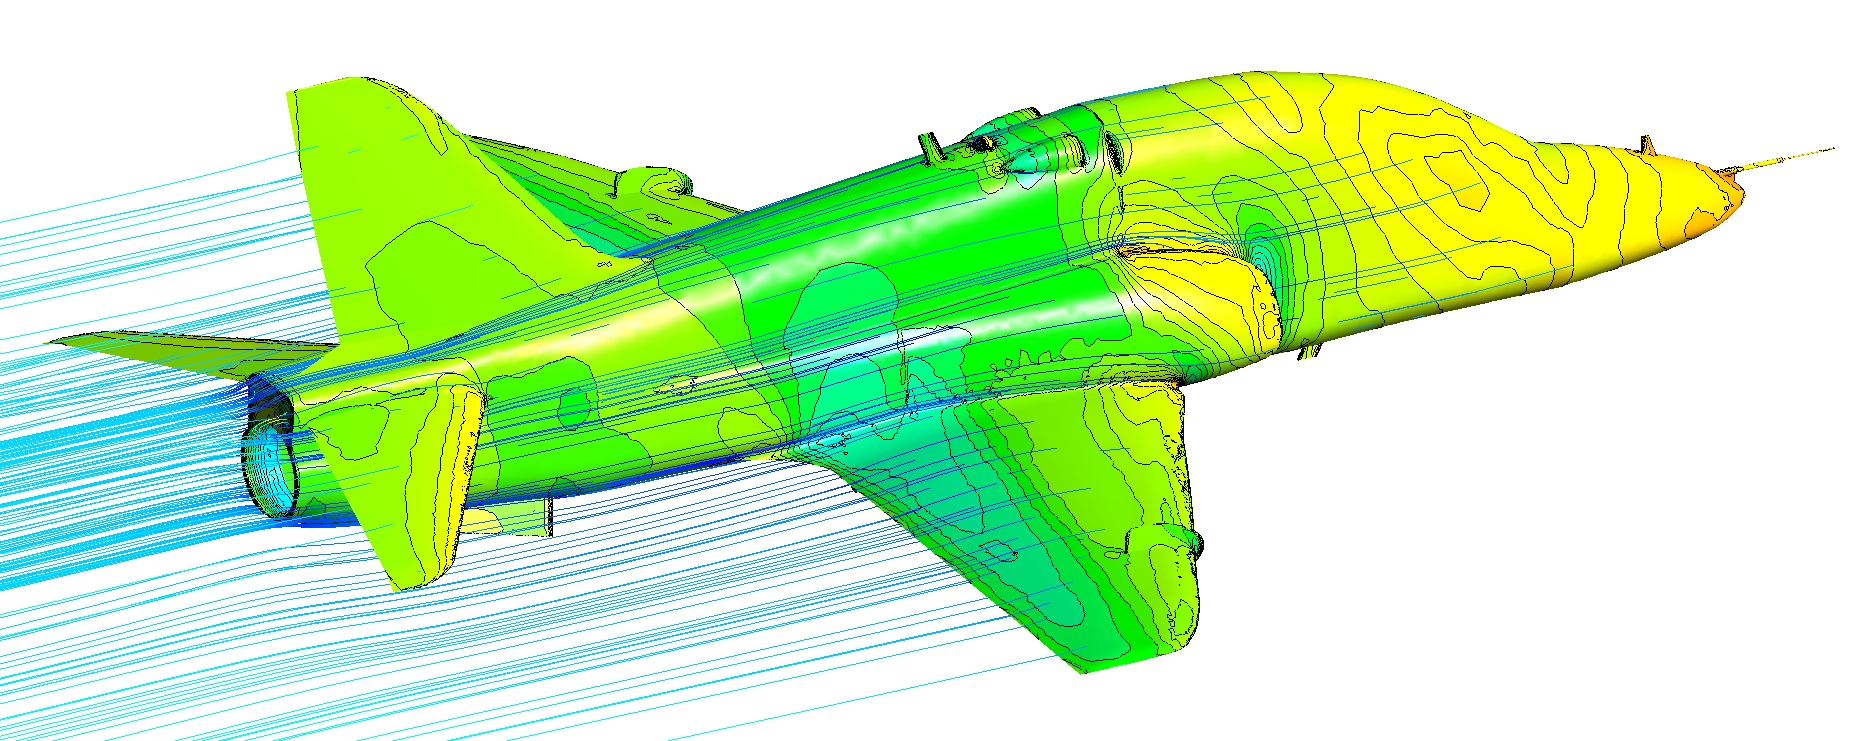
\includegraphics[width=0.7\textwidth]{1_introduction/cfd_plane.png}
    \caption[Fluid dynamic on a BAE-HAWK plane]{Fluid dynamics on a BAE-HAWK plane\protect\footnotemark}
    \label{fig:1_introduction:plane}
\end{figure}

\footnotetext{Image from \url{https://cfd2012.com/aircraft-design.html}}

\begin{figure}[!ht]
    \centering
    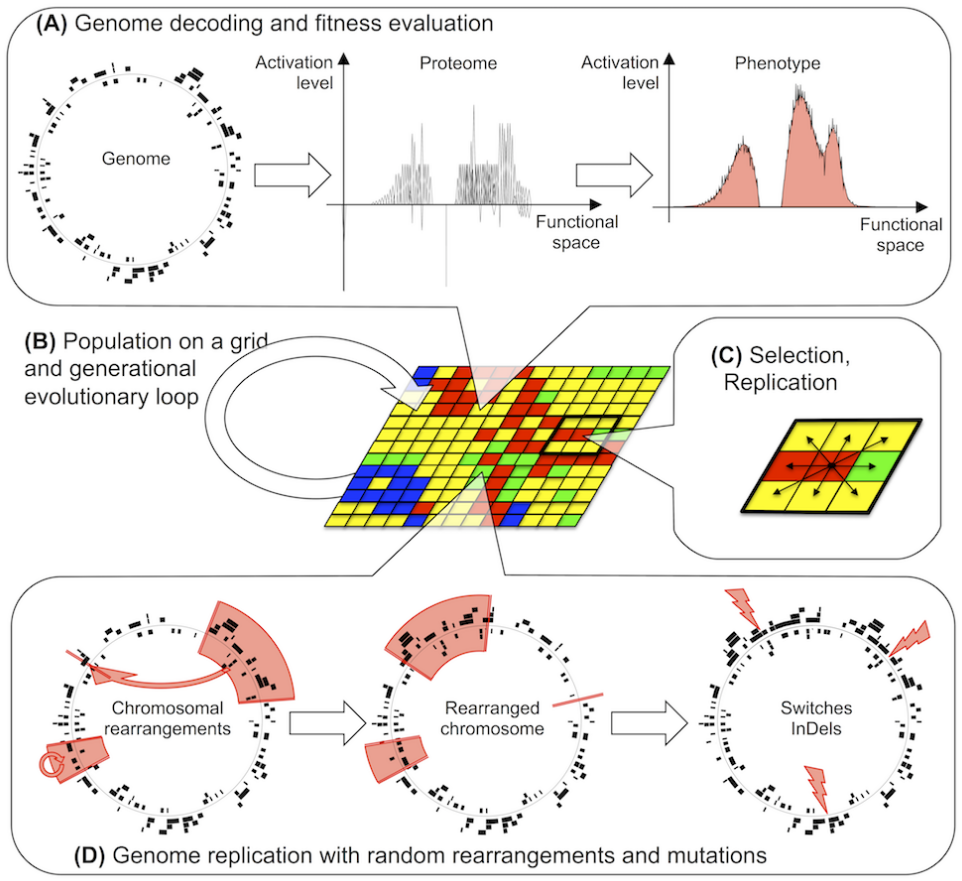
\includegraphics[width=0.9\textwidth]{1_introduction/aevol.png}
    \caption[The Aevol model]{The Aevol model. Image from~\cite{aevol}.}
    \label{fig:1_introduction:aevol}
\end{figure}

As scientific models get more and more accurate, they also become increasingly
complex, and they require an increasing amount of computing power to run. As a
result, most scientific domains today require the use of High Performance
Computing (HPC): clusters of an ever-growing number of machines which work
together towards the same goal. HPC is such a powerful tool that it is used in
most research fields, but also most industries, with applications as varied as
healthcare, weather forecast, geology, every vehicle's design, etc. An example
of such computing cluster is displayed on Figure~\ref{fig:1_introduction:ECMWF},
where we can see the supercomputing facility of the European Centre for
Medium-Range Weather Forecasts (ECMWF) in Bologna, which is made up of Atos
BullSequana XH2000 clusters and is used to run a global Earth system model, in
order to get weather reports as accurate as possible. Additionally, as
artificial intelligence takes an increasing space in our lives, through a huge
diversity of algorithms, the amount of data that we need to process is growing
at a very high rate, and the computing power required to train algorithms
increases proportionally.

\begin{figure}[!ht]
    \centering
    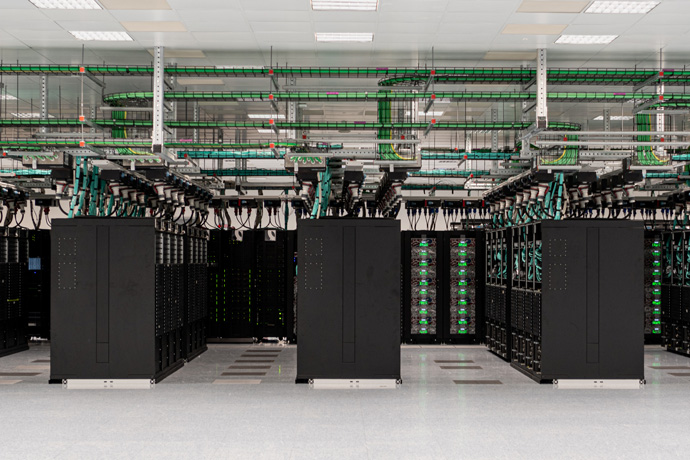
\includegraphics[width=0.7\textwidth]{1_introduction/ECMWF.jpg}
    \caption[HPC facility at ECMWF, made up of four Atos BullSequana XH2000 clusters]{HPC facility at ECMWF, made up of four Atos BullSequana XH2000 clusters\protect\footnotemark}
    \label{fig:1_introduction:ECMWF}
\end{figure}

\footnotetext{Image from \\
\url{https://www.ecmwf.int/en/about/media-centre/focus/2022/fact-sheet-supercomputing-ecmwf}}

As clusters get larger and larger, interconnection networks that connect the
machines together need to handle huge quantities of communications, with the
highest performance possible, in order not to slow down the scientific
applications running on the cluster. In this context, Atos develops its own
interconnection network, the Bull eXascale Interconnect (BXI), which is used in
some of the most powerful European supercomputers, such as
Tera-1000-2~\cite{top500_tera1000} which was the most powerful supercomputer in
Europe at the time of its installation.

Because of the growing complexity of the hardware that is used to power
supercomputers (CPUs, accelerators, interconnection network, etc.), predicting
the execution time of a scientific application on a given cluster is a difficult
task, although it is important for several reasons: for example to dimension new
clusters, or to tune the parameters of the software stack and of the hardware to
optimize performance. Additionally, designing next-generation hardware is
increasingly hard, as we constantly aim for better performance, therefore
conducting studies in simulation is a good tool to facilitate this design
process. This is where simulation can help, by providing a model of the cluster
which can be used to estimate its performance in various scenarios, even
hypothetical ones that cannot be reproduced with the hardware currently
available. This typically happens in the context of the co-design of
next-generation hardware. 

It is important to note that, since the application being run is usually itself
a physical simulation, the word ``simulation'' can be used in this context to
refer to two different objects: the simulation of a supercomputer, which uses
the cluster as the object of its study, and the simulation that might run inside
the cluster, which models a completely different system (as presented
previously). In the context of our work, our contribution is the design of a
simulator of HPC clusters (with a focus on the simulation of BXI), but in order
to validate our model we will also manipulate physics models (presented in
Chapter~\ref{chap:context_hpc}), which we will run in a virtual cluster in the
simulated world. In order to differentiate both types of simulators, in this
document we will refer to physics models as ``scientific applications'' or
``user applications'', to avoid potential confusion with our model of BXI.

In the field of cluster simulation, many types of models are available, which
are used to simulate various parts of a cluster with a high accuracy, or model
the whole cluster, but with a more simplistic model. Our work is a collaboration
between the ``Laboratoire de l'Informatique du Parallélisme'' (LIP) and
Atos\footnote{This PhD is funded by a ``Convention industrielle de formation par
la recherche'' (Cifre)}. In this context, we focus on the communication aspect
of supercomputers, and in particular on the BXI Interconnect made by Atos. Our
model of this hardware is based on the SimGrid framework, which allows us to
design a simulator modeling communications at message-level by leveraging
SimGrid's actor-based flow-model.

In the next section, we will present how BXI is designed at Atos, using our
hands-on experience with this interconnect, the knowledge that we gained from
working inside the low-level software team of this company, and our interactions
with the hardware and high-level software teams. In particular, we will present
the existing uses of simulation in this context, and illustrate the potential
benefits of a more abstract simulator.

\section{Design process of a NIC for HPC at Atos}

The process of creating an Application Specific Integrated Circuit (ASIC), such
as a Network Interface Controller (NIC) in the context of High Performance
Computing, is very costly: the full design and manufacturing process can cost
millions of Euros. Every step of the process is complex, very time-consuming and
expensive, from the design by an R\&D team, to the prototyping, and then the
actual production of the finished product. This is why this creation process
(depicted in Figure~\ref{fig:1_introduction:ASIC}) follows many steps that aim
to facilitate and speed up the design, in order for manufacturers to remain
competitive. 

\begin{figure}[!ht]
    \centering
    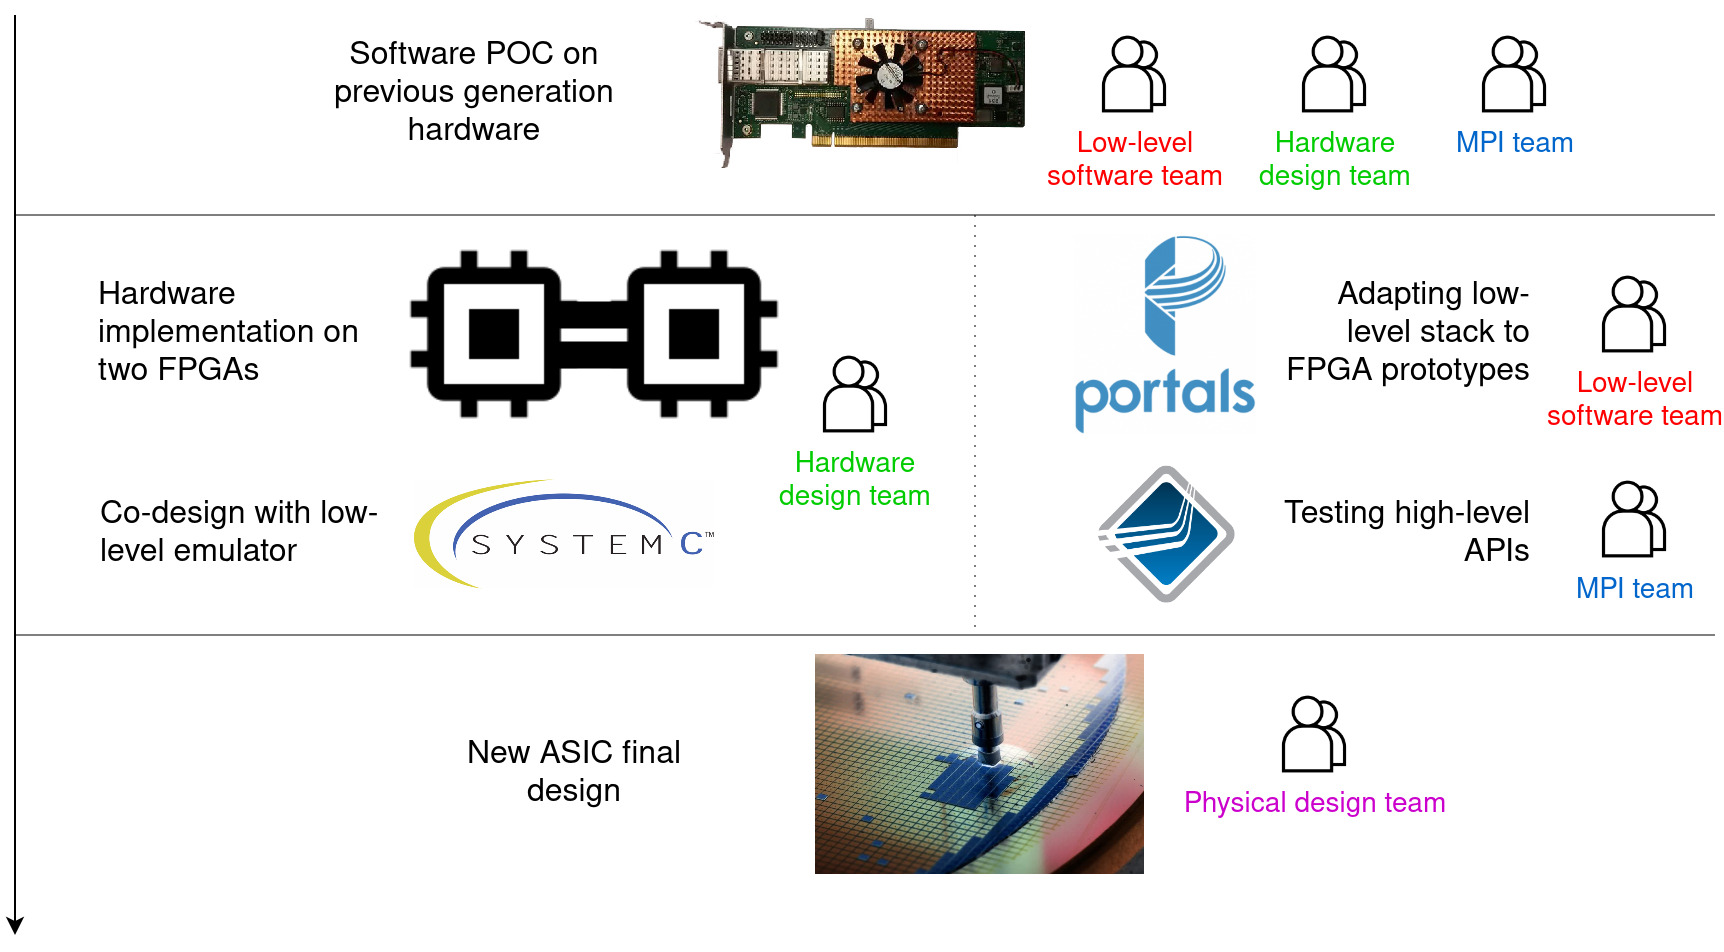
\includegraphics[width=1\textwidth]{1_introduction/ASIC.jpg}
    \caption{Design process of the BXI NIC at Atos}
    \label{fig:1_introduction:ASIC}
\end{figure}

There are mainly four teams that are involved in the process: the hardware
design is made by two teams, which are responsible for the prototyping on
Field-Programmable Gate Arrays (FPGA) and the firmware development on one side,
and the physical layout on the final ASIC on the other side. From the point of
view of the software, there are also two different teams: one of them is
specifically responsible for the tuning of Atos's version of the Message Passing
Interface (MPI), since this high-level API is the most commonly used in the
field of HPC, therefore its maintenance and optimization are very important. The
second team, BXI-LL, is responsible for the lower-levels of the software stack,
which involves developing the driver for BXI NICs, as well as the user-level
library for Portals, which is the network API implemented by the NIC. This API
offers connectionless, reliable point-to-point communications, and since it is
entirely implemented in hardware by the NIC, the user-level software library is
a very thing wrapper that mainly formats commands and sends them to the NIC.
Additionally, the BXI-LL team is responsible for the other high-level services
that are supported by BXI, such as the Lustre distributed Filesystem, OpenSHMEM,
etc.

As we can see on Figure~\ref{fig:1_introduction:ASIC}, the design process of BXI
NICs starts with an exploration of the possible features that could be
implemented, either by emulating these features on hardware that is as similar
as possible to the currently developed ASIC (for example by using old generation
hardware to design the new generation), or using a high-level simulator to get a
rough estimate of the functionality and performance of each option. Once this
step is done and the least promising features have been abandoned, the remaining
ones can be implemented in a first prototype. Because making a physical
prototype would be extremely time-consuming and costly, this step is always done
either on reconfigurable hardware such as an FPGA, or in a very low-level
simulation framework. Sometimes both are made, for example at Atos there is a
SystemC model of the BXI switch, as well as an FPGA implementation.
Additionally, in order to develop the driver and user library for the first
generation of BXI, an emulator of the NIC was made using
QEMU~\cite{bellard2005qemu}, but it was not maintained for the later generation
of BXI hardware. When the first prototype of the hardware is complete, software
developers can start using it to design the driver that is going to power the
hardware. Hardware and software developers then iterate over the prototype to
improve both the circuit and the software stack, until both are ready for
production use, which is assessed with manual tests, as well as the execution of
a test suite designed by the BXI-LL team in order to test most use-cases of the
hardware that need to be supported. At this point, the design on FPGA is passed
to a dedicated team responsible for the layout of the different circuits on the
final chip. Finally, the ASIC is ready to be manufactured at scale.

The issue with this workflow is that a prototype on an FPGA can be around two
orders of magnitude slower than the final product, especially for large circuits
where ``artificial'' bottlenecks can exist on FPGA but not on the final product:
for example the BXI NIC made by Atos does not fit on a single FPGA, and
therefore it is distributed across two FPGAs connected together. Even with this
design, the NIC must be simplified to fit on two FPGAs: only two List Matching
Engines (LMEs) can be implemented instead of four on the real ASIC for example.
These engines are Application-Specific Instruction set Processors (ASIP), which
implement most of the processing of incoming messages, with instructions
optimized to sustain a message rate as high as possible (more details about the
process of receiving messages will be presented in
Section~\ref{subsubsec:4_portals:RX}), therefore having only two on the FPGA
platform instead of four on the final ASIC is a change that has a significant
impact on the behavior of the NIC. With prototypes this slow, it is also
impossible to generate enough traffic to cause meaningful congestion on the
network, which is problematic because congestion is an important phenomenon to
study, as it impacts greatly the performance of networks with real ASICs.
Low-level simulators are even slower than FPGA prototypes, with speeds that are
often several orders of magnitude slower than the final product. This means that
during this development process, software teams can only test their code on very
small scale tests (usually involving two machines at most in the case of NIC
development). This is a problem because it makes it very difficult to evaluate
the performance of the new hardware on a realistic application, which can
exhibit unexpected behavior and performance because of the complex interaction
between all the components of a modern cluster. For example, at a small scale an
application might be CPU-bound, but at a larger scale communications might
become more important and stress the memory, which could become the bottleneck
since it is a shared resource between the CPUs and NICs. This problem becomes
even more complex if a storage system or an accelerator uses the memory at the
same time, or if the data that needs to be sent on the network is on the
storage. All of these scenarios create interdependencies between the different
resources, and their impact on performance at different scales can be
unexpected.

This is why it would be beneficial for the different development teams to have a
model of the new hardware at an intermediate level: more accurate than the
initial rough approximations, but faster than low-level emulators, in order to
study more realistic workloads. The hardware and low-level software team at Atos
could use it to perform studies on specific properties of the hardware, for
example evaluating the impact of different protocol design choices. The teams
responsible for the development of Atos's version of MPI could use it for
higher-level studies, such as tuning the algorithms used by MPI to perform
complex operations between many machines, or testing their developments.
Finally, Atos's clients could use our simulator to evaluate the performance of
their applications, and tune the configuration of their code before performing
real-world executions. In particular, the main client of the BXI Interconnect,
the ``Commissariat à l'Énergie Atomique et aux Énergies Alternatives'' (CEA)
showed interest in our work, and could be a potential user of our simulator.

\section{Contributions}

In our work, we design a simulator of HPC clusters, that is focused on the
simulation of the BXI interconnect made by Atos. As BXI NICs implement the
Portals API in hardware, we propose an implementation of this API in simulation.
To this end, we rely on the SimGrid framework, which provides a flow-model of
communication, and allows us to implement a Discrete Event Simulator (DES) using
cooperative Actors. Even though flow-models are typically used to simulate
communication at message level, we use a novel approach that models transfer at
a lower level of granularity than most state-of-the art simulators. This design
choice allows us to create a more accurate model of the hardware, without
modeling each packet individually. To the best of our knowledge, this is the
first time that a model of Portals has been made publicly available. We validate
our model, using low-level experiments which rely on the Portals API.

We show that our simulation method is versatile, by running high-level network
APIs on top of our low-level model. In this context, we study in detail the
execution of Atos's implementation of MPI in our simulator, and we also show
preliminary work with OpenSHMEM. To validate our model in this context, and to
compare it with the closest state-of-the-art MPI simulator, SMPI, we run
unmodified scientific applications that are commonly used to assess the
performance of HPC clusters. These experiments confirm our expectations, as we
observe that our simulation method is more accurate than SMPI, but also slower,
as our model is more detailed. Therefore, we explore a new method to tune the
ratio between performance and accuracy of our simulation method, by combining
our network model and SMPI's, and enabling users to switch between them at
runtime.

We conduct a study in order to assess the usefulness of potential evolutions of
BXI NICs, by implementing flow-control mechanisms in simulation and testing this
feature in different scenarios. This study shows the versatility of our
simulator, as it demonstrates how low-level features of the hardware can be
evaluated using high-level benchmarks, and we present a few other studies which
could be conducted using a similar methodology (but which are left as future
work).

\section{Structure of this thesis}

Our contributions are organized in seven chapters:
Chapter~\ref{chap:context_hpc} gives context regarding the field of HPC, by
presenting the architecture of a typical HPC cluster and the most significant
interconnection networks. It also details properties of the Portals API which
will be important for the rest of our work, and describes a few scientific
applications which will be used in our experiments.

Chapter~\ref{chap:biblio_simu} presents pre-existing simulators of HPC clusters,
with a focus on SimGrid in order to illustrate the most important features which
we leverage in our simulator. 

Chapter~\ref{chap:low_level} then focuses on our
low-level model, by explaining how Portals is implemented in simulation, and
which properties of the hardware are modeled by our approach. It also shows
validation results by relying on point-to-point benchmarks of Portals. Even
though this work was published in~\cite{Emmanuel2020a}, in this thesis we also
present several features of our simulator which were added after the initial
publication. 

Chapter~\ref{chap:high_level} explains how this model can be used to run
high-level APIs, and in particular MPI. To this end, it details the
modifications that need to be performed on the real-world implementations of MPI
and OpenSHMEM in use at Atos, in order to make them compatible with our
simulator. Part of this work was published in~\cite{Emmanuel2021}, but
significant work has been added since: in particular, this publication does not
mention our study on OpenSHMEM, and our benchmarks are now more complete.

Chapter~\ref{chap:model_change} shows how we can combine two network models, and
allow users to switch between them at runtime. 

Chapter~\ref{chap:flowctrl}
discusses some ideas that are more experimental, in particular it details our
study on flow-control in BXI (a very early version of this work was published
in~\cite{Emmanuel2021}), and it lists ideas that are left as future work.

Finally, Chapter~\ref{chap:conclusion} concludes this document by summarizing
our work.


\chapter{Context: High Performance Computing}
\label{chap:context_hpc}

This chapter presents the context of our work. We will start with an overview of
the architecture of a modern HPC cluster, and then showcase several benchmarks
commonly used in HPC, which we will refer to later in this thesis (in the
context of the validation of our simulator).

\section{HPC clusters' architecture}

Our work focuses on the network aspect of High Performance Computing. We will
start with some context regarding HPC clusters, and then focus on the challenges
that interconnection network face, both at the hardware and software level.

\subsection{General overview}

Because of the physical limitations that CPUs face, High Performance Computing
(HPC) clusters use very specific hardware to get the most computing power
possible from each machine that composes the cluster, and they also have an
increasing number of machines connected together. This means that a typical
machine (referred to as ``node'' in this document) is usually composed not only
of one or more CPUs, but also one or more Network Interface Controller (NIC) and
possibly one or more accelerator for fast parallel computation. These nodes are
interconnected using switches of low-latency and usually high radix (i.e. a large
number of ports allows connecting many nodes or other switches), which enables
various topologies to be used. For example
Figure~\ref{fig:2_context_hpc:FatTree} depicts a simple fat-tree, with wider
links (higher bandwidth) closer to the ``root'' of the tree. On this example, we
can see that the distance between two nodes is variable: two machines connected
to the same switch will be able to communicate by traversing only two cables and
one switch, whereas nodes on opposite sides of the tree will need to traverse
four links and three switches to communicate, increasing the latency of network
transfers.

\begin{figure}[!ht]
    \centering
    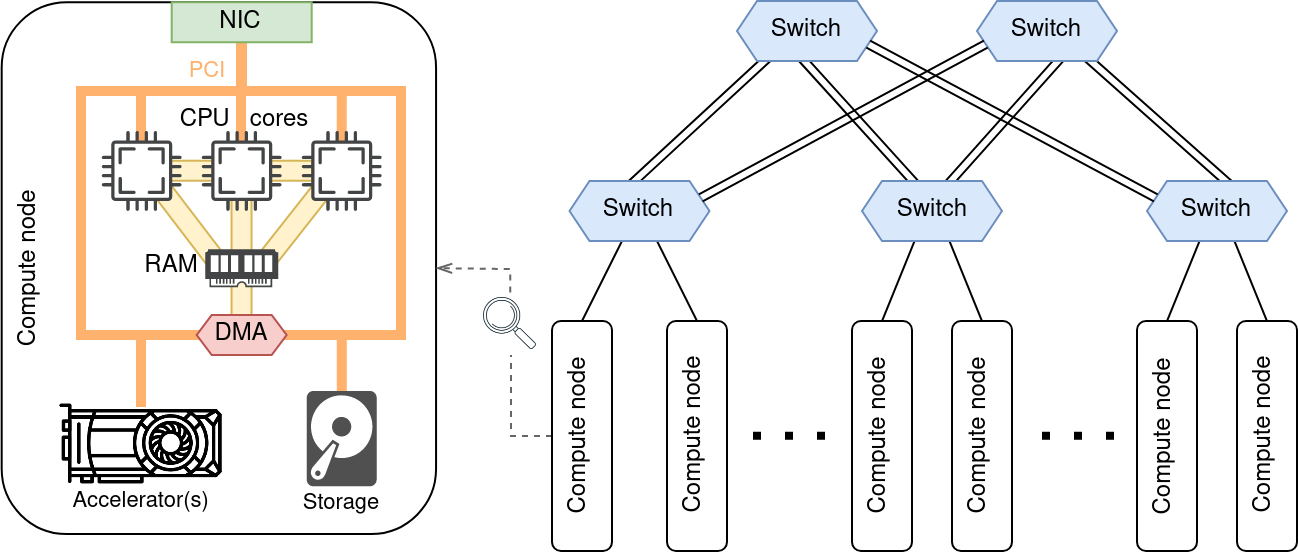
\includegraphics[width=1\textwidth]{2_context_hpc/fat_tree.png}
    \caption{Simplified cluster representation, with a zoom on a compute node}
    \label{fig:2_context_hpc:FatTree}
\end{figure}

While the diversity of hardware and increasing number of nodes makes clusters
more performant, it also makes it more difficult to predict the performance of a
cluster executing a given application, because of complex interactions between
each type of hardware on each node. A second side effect is that clusters become
increasingly more costly to build and run, which makes real-world experiments
very costly. The increase of the number of nodes also makes the topology of the
cluster more and more important: routers and cables are an expensive part of the
cluster, but it is crucial that they have a good performance, so connecting all
this hardware efficiently is very important. On
Figure~\ref{fig:2_context_hpc:FatTree} we can see that while nodes are usually
very similar to each other (a typical cluster will have many identical compute
nodes, and a few service nodes for login, storage, management, etc.), the
allocation of tasks on the cluster still matters, because of communications:
nodes that are on different switches will have to go through more links and
switches in order to exchange data, whereas nodes on the same switch will
benefit from a very low latency. We can also see that messages can take several
paths through the network when going from one node to another, which makes
efficient routing important.

There has been many studies in the field of interconnection networks and routing
algorithms, from which many topologies have emerged. To cite only the most
commonly used, the Flattened Butterfly~\cite{Kim2007} focuses on
cost-efficiency, by relying on path diversity, which shows the best result when
the routing algorithm used leverages adaptive routing, which means that switches
can decide which path to choose on a message-per-message or packet-per-packet
basis, instead of having a strict static route for each source-destination pair
(which improves the load-balancing abilities of the network).
Dragonfly~\cite{Kim2008} networks operate on the same idea, but they use groups
of switches to emulate a ``virtual router'' of even higher radix than the
underlying switches, which further reduces the cost of building the network,
while still showing good performance. Torus~\cite{Ajima2009} topologies are more
original since they do not use a traditional architecture with NICs on compute
nodes and switches to connect them together: instead every node has an
``interconnect controller'', which acts both as a NIC (with several
``communication engines'' to communicate with CPUs) and a small switch (with a
dozen of ports typically). This allows nodes to be connected in small groups,
and groups to be connected together along a variable number of dimension (up to
6D for the Tofu interconnect for example). Finally, the most common topology is
probably the Fat-Tree~\cite{Leiserson1985}, which has been extensively studied,
in order to improve routing~\cite{Gomez2007}, make accurate
simulations~\cite{Liu2015}, etc. It relies on a hierarchy of switches, with
compute nodes connected at the lowest level, and cables of increasing bandwidth
as we get closer to the root of the tree, as depicted earlier in
Figure~\ref{fig:2_context_hpc:FatTree}. Several routing algorithms have been
proposed on this topology, which rely on either static or adaptive
routing~\cite{Gomez2007}, and which try to balance the load as well as possible
between the different paths that are available in the tree. The most common is
D-Mod-K~\cite{Zahavi2010} but others exist, such as node-type-based
load-balancing~\cite{Gliksberg2018} which was proposed by Atos.

While our work could theoretically be used to study different topologies and
compare their performance, it will not be discussed in  detail in this thesis
because the interconnect that we work on, BXI, is mostly used with Fat-Trees in
production, therefore all our experiments will use this topology.

\subsection{Networking hardware}

In the world of High Performance Computing, there are several competitors when
it comes to production interconnection networks: the most notable are Cray
(acquired by HPE during this PhD), Mellanox (acquired by Nvidia during this
PhD), Fujitsu and Atos. Another noteworthy interconnection network is OmniPath:
while it has first been discontinued by Intel, it has since been bought by
Cornelis Networks, and there are several interesting studies on its performance
and modeling~\cite{Rosales2017}.

Cray's interconnects support a wide range of topologies: from Dragonfly network
in their latest Slingshot interconnect, to 3D-Torus in the Seastar
interconnect~\cite{Brightwell2005}. Torus networks have been shown to work in
higher dimensions, for example in 6D with the Tofu interconnect~\cite{Ajima2009}
made by Fujistu, which is used in the Fugaku supercomputer (number two on the
Top500 list as of the writing of this PhD). While early versions of Cray's
interconnect were known to use Portals 3 as their lower-level network API,
Slingshot is based on the Ethernet protocol~\cite{DeSensi2020}. On older
generations of interconnect (as the Gemini and Aries which are still used in
several clusters) the lowest software layer that is exposed to user code is
composed of two APIs: uGNI and DMAPP~\cite{Cray2010}. Cray's NICs typically
support bandwidths up to 200Gbits/s.

Mellanox's interconnects are the most popular option for new clusters. They
implement the standard Infiniband architecture~\cite{Pfister2001}, which is
supported by most (if not all) higher-level APIs. They also feature a variety of
hardware of different performance and price, such as the EDR and HDR series,
which explains their popularity for clusters of all sizes. At the
lowest level, users call the IB-verbs interface which is used to communicate
with the NIC. High-end NICs from Mellanox typically support bandwidths up to
200GBits/s, with the upcoming generation expected to support 400Gbits/s.

Atos's interconnect, BXI, will be our case study for this PhD. It implements in
hardware the Portals 4 network API, and is used in some of the fastest European
supercomputers. It is one of the youngest interconnect of the market, with NICs
supporting bandwidths up to 100Gbits/s, but it has showed very good results so
far, equipping supercomputers with a very good rank in the Top500 list:
Tera-1000-2 was at the 14\textsuperscript{th} place worldwide and n°1 in Europe
at the time of its installation~\cite{top500_tera1000}, and currently Exa1-HF
holds the 20\textsuperscript{th} place worldwide~\cite{Top500_exa1} (it was also
14\textsuperscript{th} at the time of its installation in 2021).

All these interconnects share a few similarities: their main goal is to offload
as much network processing from the CPU as possible. This is made possible using
a few properties that differ from traditional networking hardware: first,
OS-bypass allows user code to send commands to a NIC without any system call,
which speeds up communications significantly. Most NICs also provide zero-copy
processing, which implies that incoming messages can be processed fast enough so
that the incoming data is routed to the correct location in memory without being
copied in intermediate buffers. This is made possible either by pinning memory
pages used for network communications (as Mellanox's hardware does), or by
having a full Virtual-to-Physical (V2P) circuit on the NIC (as does Atos's BXI
hardware).

While the simulation of other interconnects and network APIs have been studied
in depth, for example the congestion on Infiniband networks
by~\cite{Vienne2010}\cite{Gran2012}, Intel OmniPath with
OpaSim~\cite{Javier2018}, or Cray's interconnect~\cite{Mubarak2017}, very few
studies have been conducted on BXI, and the existing ones focus on very specific
problems, such as the update of routing tables when the topology
changes~\cite{Vigneras2016}. In this thesis we will propose a model for Portals
4 and tune the simulator for accurate simulations of the BXI interconnect.

\subsection{Networking Software Stack}
\label{subsec:2_context_hpc:software_stack}

While the typical software stack for HPC communications is very different from
the traditional OSI layers, it features similar levels of abstraction (depicted
on Figure~\ref{fig:2_context_hpc:HpcSoftwareStack}). We will start by giving a
global overview of these layers, before presenting Portals in more details in
the next section, since it is the lowest-level software layer used at Atos, and
it will be the most important from the point of view of our
simulator.

\begin{figure}[!ht]
    \centering
    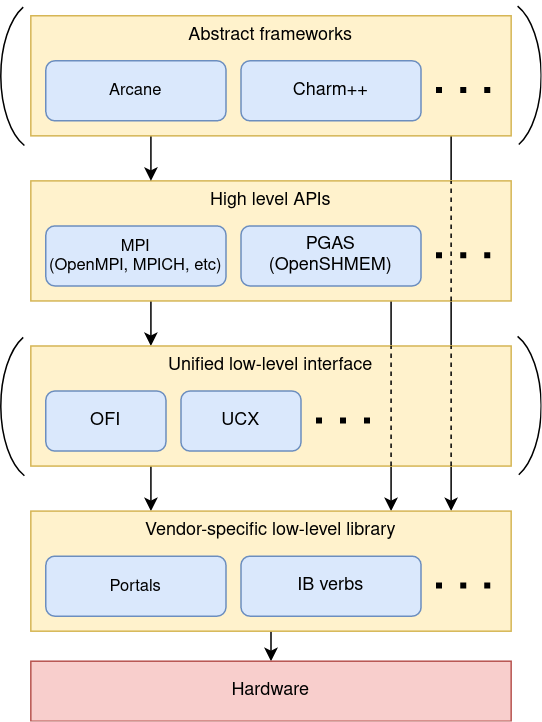
\includegraphics[width=0.6\textwidth]{2_context_hpc/HPC_software_stack.png}
    \caption{HPC software stack}
    \label{fig:2_context_hpc:HpcSoftwareStack}
\end{figure}

At the lowest level, there is usually a very thin software library (potentially
coupled with a kernel module), that directly interacts with the hardware, and
exposes a few primitives with a very low level of abstraction to user code. It
usually only performs point-to-point operations between two machines, and does
not have any notion of collective operations involving several machines. For
Infiniband this layer is called IB-verbs, and for Atos's BXI interconnect it is
the Portals 4 API directly, as it is fully implemented by the NIC in hardware.
It is this Portals 4 layer that our simulator will model, as it will provide a
model of the behavior of the NIC.

Above this layer, high-level APIs provide more abstract features that allow
programmers to write efficient code, focusing on the algorithmic aspects and
abstracting away the implementation details of communications. In this category,
several programming models exist: for example Partitioned global address space
(PGAS), with implementations such as OpenSHMEM~\cite{Chapman2010}, allow user
code to have a transparent representation of memory that is distributed on
several machines. The most popular of these programming models is without a
doubt the Message Passing Interface (MPI)~\cite{Graham2006}, which offers many
ways of communicating: onesided, where a target machine exposes memory regions
that other machines can query ; regular point-to-point operations where both
machines are actively involved (using send and receive primitives) ; and finally
collective operations which provide abstract communication primitives such as
all-to-all pattern, gather (N to 1 communication), scatter (1 to N), and even
simple data processing with reduce, allreduce, etc. primitives. These collective
operations usually have several implementations, which can be chosen dynamically
depending on the message sizes and the number of machines involved in the
operation. There are many MPI implementations, such as OpenMPI, MPICH, IntelMPI,
etc. We will study OpenMPI in particular, as it is the MPI implementation that
is officially supported by our case study interconnect, BXI. It is worth noting
that our version of OpenMPI is a fork optimized by Atos for BXI, which we will
explain in more detail in Chapter~\ref{chap:high_level}. These high-level APIs
are sometimes criticized for their cost in terms of performance, in particular
MPI~\cite{Raffenetti2017}, but their compromise between ease of use and
performance makes them the standard to write HPC applications. Some projects
even try to replicate this type of programming model in hardware,
as~\cite{DeMatteis2019} does on Field Programmable Gate Arrays
(FPGAs).

These two layers are the most important and will usually exist in any HPC
software stack, but there can also be additional ones: in particular some APIs
try to provide a unified interface between the low-level transport and the
high-level abstract API. The goal of this added layer is to limit the number of
implementations that need to be made in high-level APIs to accommodate for any
possible low-level transport. This is similar to the intermediate representation
compilers use, which allows them to have only $N$ frontends and $M$ backends to
be able to compile $N$ languages into $M$ machine codes, instead of having $N
\times M$ complete toolchains. These interfaces include the Open Fabric
Interface (OFI)~\cite{Grun}, of which Atos made an implementation built with
Portals (in order to support BXI), as well as Unified Communication X
(UCX)~\cite{Shamis2015} or Nemesis~\cite{Pritchard2011} for example.

Finally, while high-level APIs are already more user-friendly than low-level
transports, they are still very general purpose and offer much control, which is
why some frameworks can be used on top of them for even more abstraction. They
can be domain-specific, as Arcane~\cite{Grospellier2009} for example, which is a
tool made by the CEA to build physics simulators on top of MPI. Some libraries
like SkePU~\cite{Enmyren2010} provide complete data-processing algorithms on
distributed data, for example MapReduce, Stencils, etc. Some frameworks expose a
unified API to execute algorithms on heterogeneous architectures (for example by
exploiting local parallelism with OpenMP\footnote{OpenMP is an API for parallel
processing across CPU cores, which relies on compiler directives and a library},
inter-machine parallelism with MPI, etc.) like StarPU~\cite{Augonnet2011}. Some
approaches even go as far as designing a full programming language for parallel
processing, such as Chapel~\cite{Parenteau2021}, which implements a PGAS model
and uses low-level transports directly, or Charm++~\cite{Kale1993}, which
provides automated load balancing and supports MPI as its transport mechanism.

\begin{figure}[!ht]
    \centering
    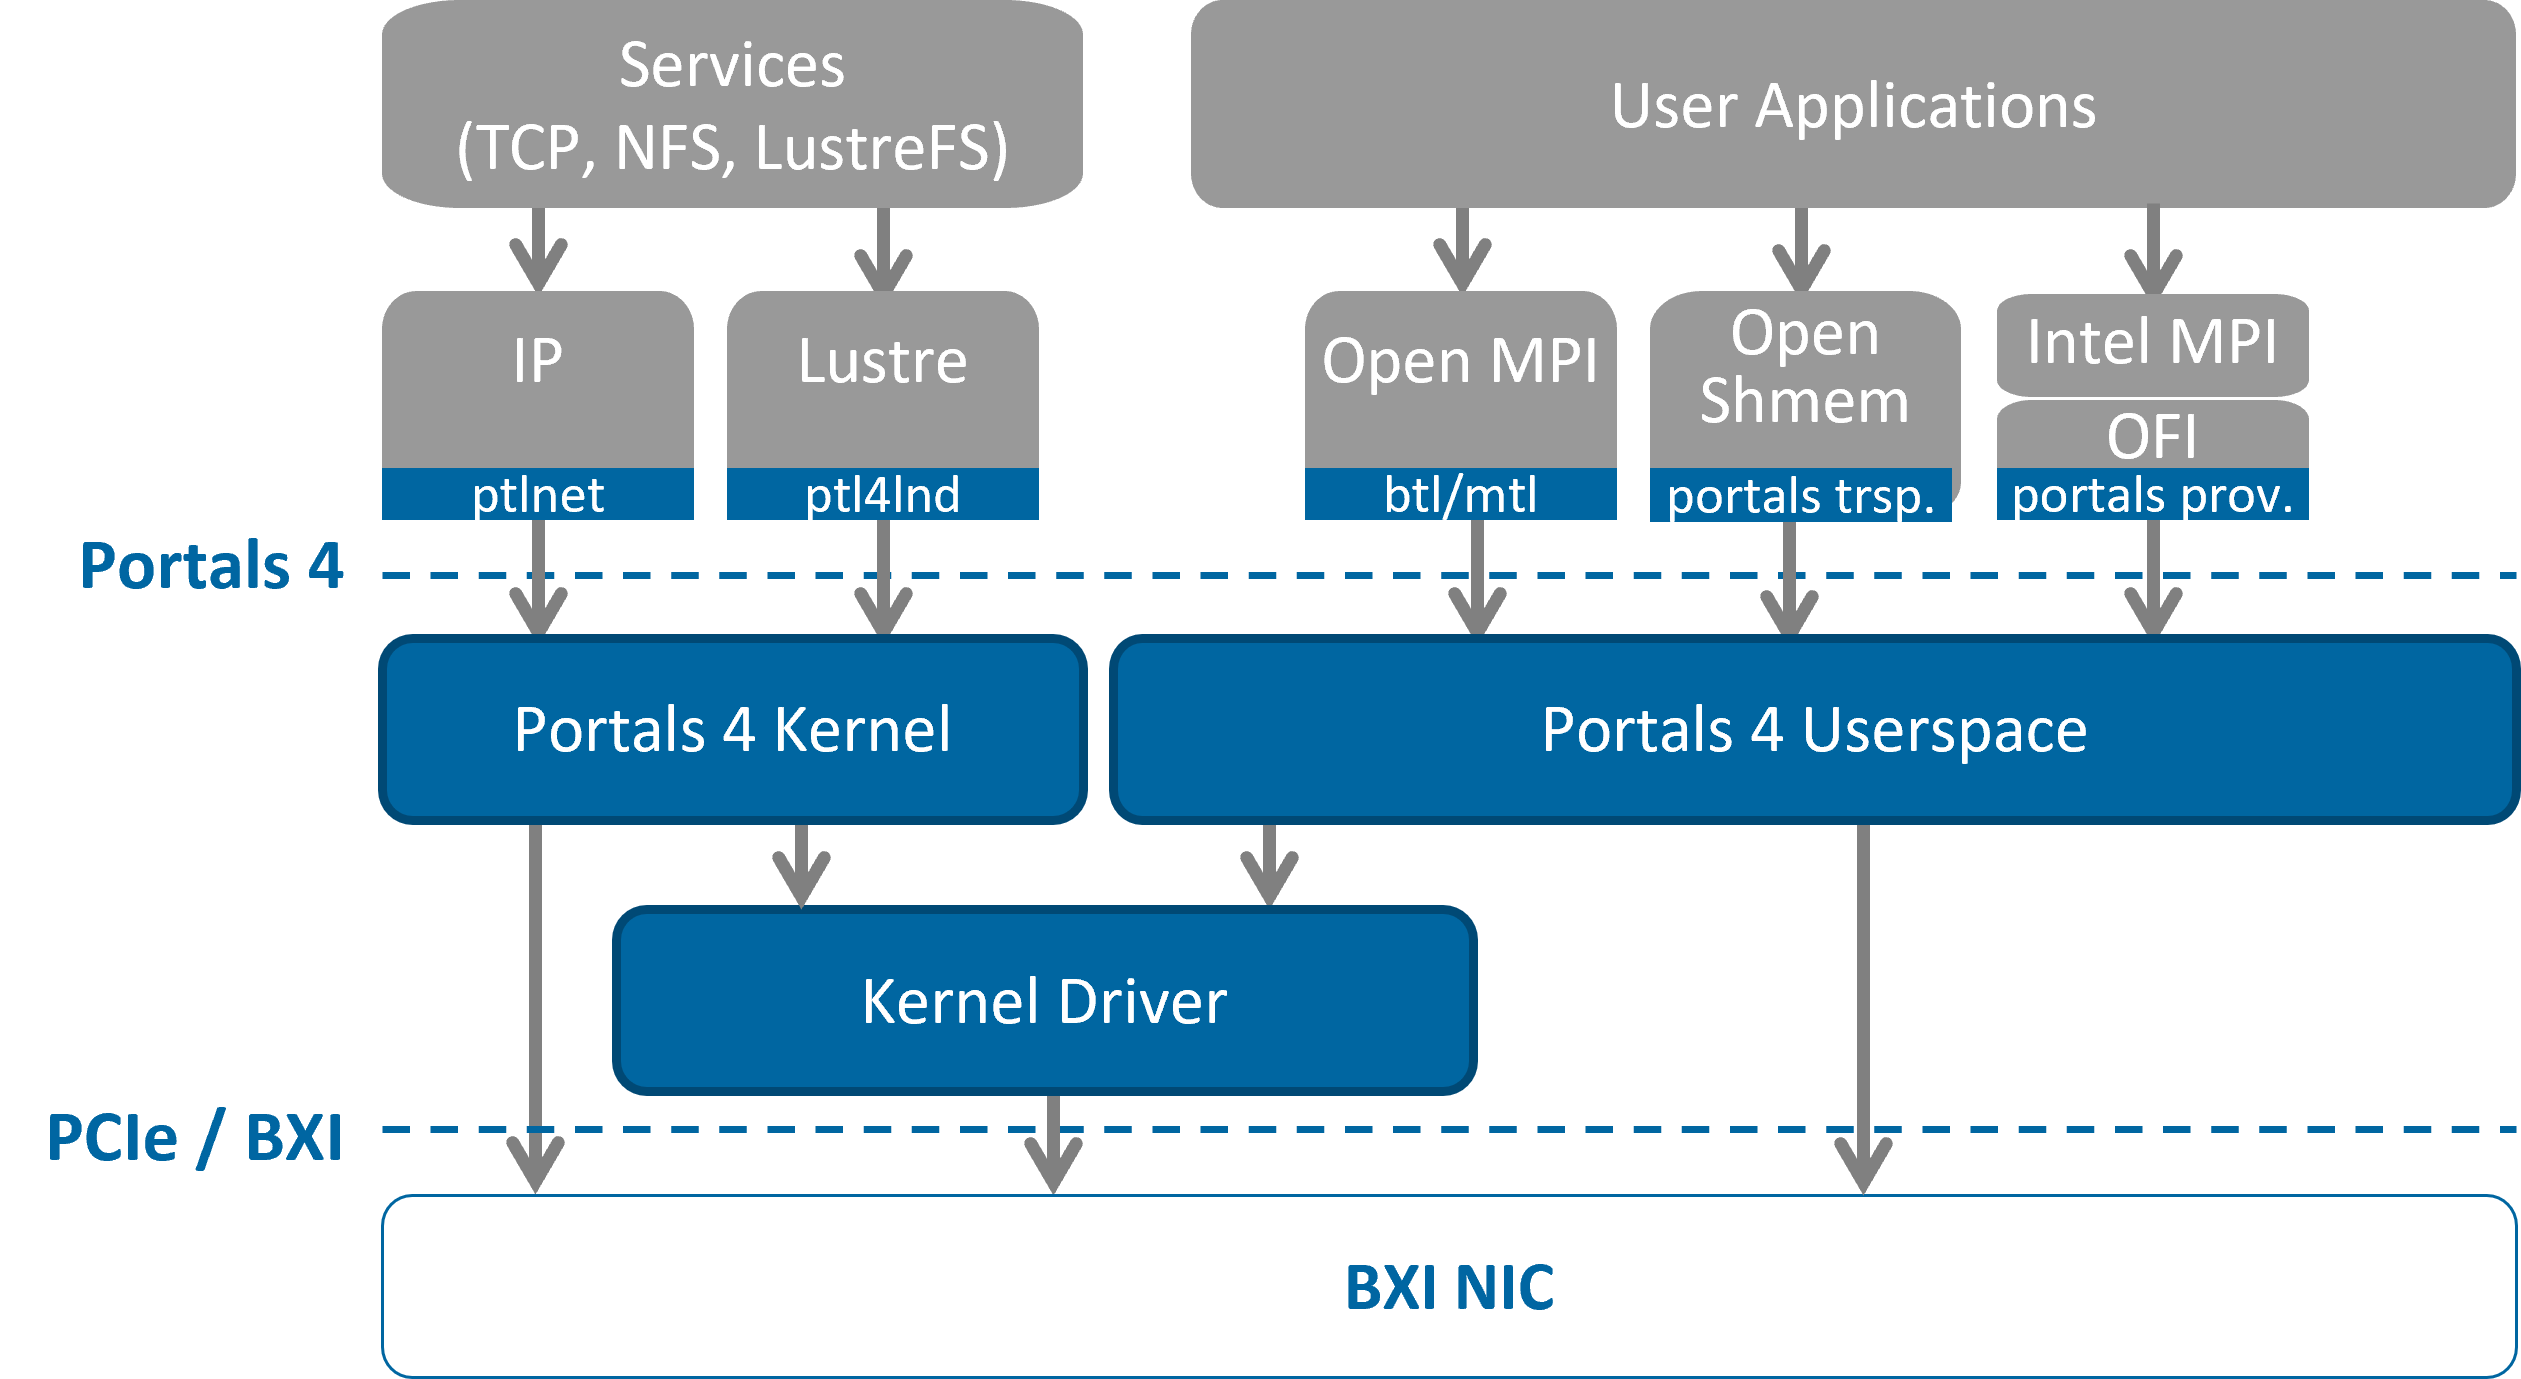
\includegraphics[width=0.9\textwidth]{2_context_hpc/atos_stack.png}
    \caption{Atos's software stack on top of BXI NICs}
    \label{fig:2_context_hpc:AtosSoftwareStack}
\end{figure}

The software stack used at Atos, which is going to serve as a case study for
this thesis, is depicted on Figure~\ref{fig:2_context_hpc:AtosSoftwareStack}. It
is based on Portals, which we will describe in more detail in the next section,
and supports a wide range of higher level APIs and services: it can emulate the
Ethernet protocol using a layer called Ptlnet, supports the Lustre distributed
Filesystem, provides different APIs for fast computation such as OpenMPI,
OpenSHMEM, and IntelMPI (on top of OFI), etc. In this thesis we will study in
detail OpenMPI in particular, and we will discuss OpenSHMEM support.

\section{The Portals API}

Portals is a standard HPC API specified by Sandia National
Laboratories~\cite{Brightwell2022}. It has been used in supercomputers for
decades, with a few success stories like the ASCI Red
supercomputer~\cite{Mattson1998}, which was the first to break the Teraflop
barrier in 1996 using an early version of Portals. Since then Portals has been
used mainly by Cray, and nowadays its main implementation is in the BXI
interconnect made by Atos. This API provides connectionless, reliable
communications using Remote Direct Memory Accesses (RDMA). While many details
about the underlying protocol are left to the implementation, Portals is
designed with OS-bypass in mind, and it should enable a ``natural''
implementation of MPI two-sided primitives, as well as PGAS one-sided
operations.

\subsection{Portals data structures}

Portals features several data structures to interact with the hardware, which
are defined in the Portals's specification~\cite{Brightwell2022}. This section
presents the most important ones in the context of our work.

\subsubsection{General purpose structures}

\portalsAbbr{Network Interfaces}{NI} act as an ``entry'' point, which represents
the interface with the hardware. In Portals the addressing is analogue to IP
addressing, since each physical NIC has a \portalsAbbr{Node Identifier}{NID},
which is the equivalent of IP addresses (although it is a simple number instead
of a full address), and each NI (which usually corresponds to a single
application process) has a unique \portalsAbbr{Process Identifier}{PID}. In
those NIs, one or more \portalsAbbr{Portal Table}{PT} stores the data structures
that will be used for the reception of messages. The pair $\{PID ; PT\}$ is
similar to ports in an IP-based stack.

\subsubsection{Reception data structure}

\portalsAbbr{Matching Entries}{ME} are used to configure the reception of
incoming messages. A matching entry stores the address and length of the memory
space where incoming messages' data should be written, as well as match bits and
ignore bits. Match bits are a set of 64 bits which allows an efficient routing
of data at the receiver side: when an initiator sends a request, it includes
match bits in the message, and the target uses these bits to identify which ME
should be used to process the request, by testing each ME against the incoming
message using the following criterion:

\begin{center}
    $((incoming\_bits \; \wedge \; match\_bits) \;\;\; \& \;\; \sim\!ignore\_bits) \: == \: 0$
\end{center}

\begin{figure}[!ht]
    \centering
    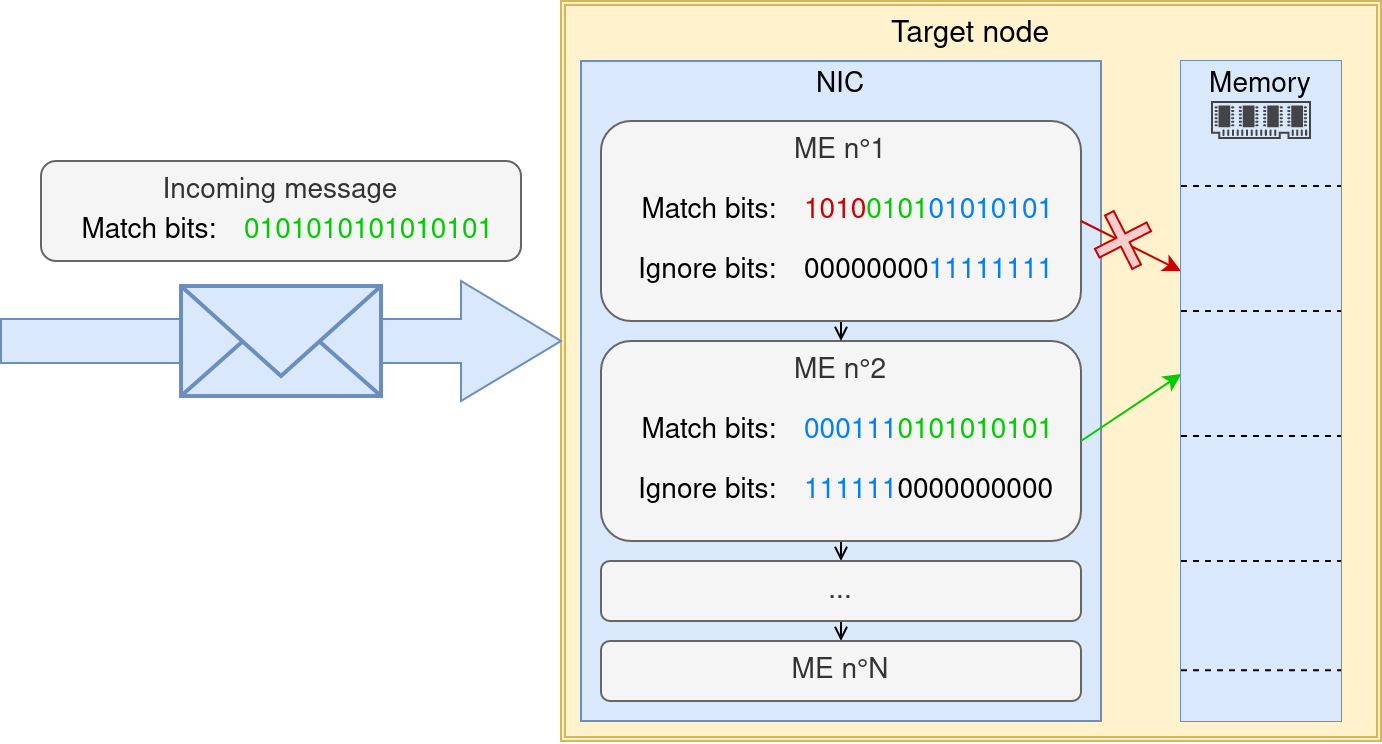
\includegraphics[width=1\textwidth]{2_context_hpc/match_bits.png}
    \caption{Example of matching between MEs and an incoming request}
    \label{fig:2_context_hpc:matching}
\end{figure}

The first ME to match the incoming request is then used to determine on which
memory region the requested operation needs to be performed. An example is shown
on Figure~\ref{fig:2_context_hpc:matching}, where we can see that nodes can have
several MEs, which map to different locations in memory. To determine which ME
needs to be used when processing an incoming request, Portals loops through the
available MEs, and looks at match bits, using the opposite of the ignore bits as
a mask (so the only match bits that are relevant are the positions where there
is a 0 in the ignore bits). If those bits are the same as in the incoming
message, the ME is used to process the message (in order to determine the memory
location where the incoming payload should be written). In the example, the
first ME does not match, because the first bits are not ignored and they are
different from the first bits of the incoming message, whereas the second ME
matches because even though the first bits are different, they are ignored, and
all the ending bits are identical to the bits of the incoming message.
Therefore, the payload from the incoming message is stored in the memory
location referenced by ME n°2.

MEs feature a variety of options that affect their behavior: they can have one
or several uses, as well as locally manage the offset at which messages are
written after each operation (by default this offset is specified on the sender
side), etc. Portals also features more simple \portalsAbbr{List Entries}{LE},
which function exactly as MEs, but do not use match bits or ignore bits, which
means that every incoming message will match the first LE posted in the Portal
Table.

\subsubsection{Transmission data structures}

The data structure for transmission is more simple than the structures for
reception: \portalsAbbr{Memory Descriptors}{MD} are simply used to represent the
start and length of the memory zone that needs to be sent on the network. They
also feature a few options, but which do not change drastically their behavior:
these options mostly impact which events need to be emitted or not.

\subsubsection{Event systems}

Portals feature two distinct event systems, which allow users to be notified of
the activity on the network by attaching data structures to a PT, an MD or an
ME.

The first, more complete system involves \portalsAbbr{Event Queues}{EQ}, which
record full events with detailed information on the corresponding operation,
such as the type of event, an error code, and a variable number of fields
depending on the type of the event (for example the NID of the remote peer who
caused the event, or the amount of data that was impacted, etc.). EQs can be
associated with PTs and MDs.

The second system is more lightweight: instead of EQs, it uses
\portalsAbbr{Counting Events}{CT}, which do not record any information about the
operations that is in progress. Instead, each CT features two counters that
track successful operations and failed operations. CTs can either count by
incrementing by one each time, or incrementing by the number of bytes that was
manipulated in the corresponding operation (based on a flag at their creation).
CTs can be associated with MEs and MDs.

Both systems can be queried through a variety of function, which can search for
events (or a certain value in CTs) in a way that is either asynchronous or
blocking, while looking at either one or several EQ/CT.\newline

\subsection{Communication primitives}

Portals features several operation types to exchange and manipulate data. All
these operations are strictly point-to-point, as Portals does not have a concept
of collective operation.

\subsubsection{PtlPut}

Put operations are a very basic ``send'' operation, which corresponds to an RDMA
write. As most operations, it can have match bits or not, and it will trigger
various events that users can listen to: in particular a ``SEND'' event when the
user buffer (which contains the data to be sent) can be safely re-used and an
``ACK'' event when an acknowledgement has been received from the remote node
that was targeted. At the target, Put operations trigger a ``PUT'' event.

\subsubsection{PtlGet}

Get operations correspond to an RDMA read: making a Get request only sends a
small message to ask the remote machine for a piece of memory, at which point
the remote NIC will send back the requested data in a response. Unlike Put
operations this means that the request is very lightweight (only a few bytes of
metadata) and the payload which can have an arbitrary size is in the response
instead. From a user perspective, the completion of the operation can be tracked
by listening to a ``REPLY'' event. At the target, Get operations trigger a
``GET'' event.

\subsubsection{PtlAtomic}

Atomic operations operate in a way that is very similar to a Put, but the NIC
also performs an arithmetic operation using two operands: the incoming payload
and the data already present at the specified address in the remote node's
memory (which is also used to store the result). These operations can be a sum,
product, etc. on various data types (integers, floating point numbers, etc.).

\subsubsection{PtlFetchAtomic}

FetchAtomic operations work in the same way as Atomics, but they also send a
full response which contains the piece of data before it was modified by the
Atomic operation. This means that FetchAtomic behaves as an Atomic and a Get at
the same time: the request contains data to be used by the Atomic operation, but
the response also contains data to be written at the initiator side as in a
traditional Get. This also means that the operation involves two MDs at
initiator side: one to describe the data to be sent and one to store the
incoming response.

This operation has a variant, called PtlSwap, which operates very similarly to
\inline{PtlFetchAtomic} except that the permitted operation types are not
arithmetic operations but different variations of swaps (conditional, with a
mask, etc.).


\subsection{Portals's implementation in BXI}

While Portals is a good specification for the API that should be exposed to
users, at the lowest level significant freedom is left to the implementation. In
this section we will present a few properties of BXI's implementation of Portals
which will be of interest when modeling Portals in our simulator.

\subsubsection{End-to-End (E2E) Reliability}
\label{subsubsec:2_context_hpc:E2E}

Since Portals is a reliable network API, it is the responsibility of BXI NICs to
ensure that messages are delivered without errors. At packet-level the integrity
of the data is enforced using a Cyclic Redundancy Check (CRC): each network
packet features a field in its header for CRC data, which allows the receiver of
messages to check the integrity of the payload, and send an acknowledgement
(ACK) with an error code if any packet was corrupted, which will trigger a
retransmission of the message by the sender. At message-level, a system of
timeouts and retries is implemented using a dedicated ``E2E'' circuit. This part
of the NIC keeps track of all outgoing messages, and if no acknowledgement is
received within a configurable delay, the NIC will retransmit it. This happens a
tunable number of times until the message is eventually given up on. An
interesting property to note is that since ACKs are important messages that need
to be reliably transmitted to ensure all events are properly generated, BXI
implements two levels of ACKs. We will call ``Portals ACK'' the messages that
acknowledge the reception of a Put or Atomic operation (which can cause the
emission of an ACK event for the user application), and ``BXI ACK'' the messages
that acknowledge the reception of a Portals ACK (which is only used internally
by the E2E logic to know that a Portals ACK message does not need to be
retransmitted, in a way that is entirely transparent to the user application).

\subsubsection{Virtual Networks (VN)}
\label{subsubsec:2_context_hpc:VNs}

According to the Portals specification, it is required for messages to be
ordered. This means that commands issued to the NIC by the user should result in
messages being sent on the network in the same order, and also that this order
should match the order of receptions at the target (in case all messages target
the same machine). This causes a practical issue in real-world scenarios, which
can lead to a complete deadlock of a NIC in the worst case: for example if
fetching the data that needs to be sent by a request triggers a page fault which
can only be resolved with another Portals request (if this data is located on a
Network File System for example). Such dependencies between requests are solved
by allowing different VNs to progress independently: BXI supports a total of
four VNs: a ``COMPUTE'' VN for requests, a ``COMPUTE'' VN for responses, a
``SERVICE'' VN for requests and a ``SERVICE'' VN for responses. In our previous
example, the problem would be solved by starting the NFS in ``SERVICE'' mode
while having the main application in ``COMPUTE'' mode.

This system also allows requests and responses to progress independently: for
example a small ACK can progress even if a large request is in progress. This last
property is to be taken with a grain of salt: even though the vast majority of
the processing in the NIC allows all four VNs to progress independently, at the
very end (writing the packets physically on the network cable) messages are once
again sequential, and packets from different messages cannot be
interleaved.

\section{Benchmarks of interest}
\label{sec:2_context_hpc:benchmarks}

In HPC, there is a wide variety of benchmarks that are used to assess the
performance of a cluster. The diversity of these applications comes from the
need to evaluate performance at different scales, for example with low-level
utilities to evaluate the speed of communications between a pair of machines, or
at the opposite full scale applications which exhibit more complex behavior but
which are also a more realistic use-case of an HPC cluster. Benchmarks can also
have different goals in terms of workload: some are more network-intensive,
others will focus on CPU usage, etc. The original use-case of most benchmarks is
to evaluate the performance of real clusters. In contrast, this thesis focuses
on simulation, and we will use the same benchmarks to assess the accuracy of our
models. We will therefore run these benchmarks both on real-life clusters and in
simulation to compare the results.

Additionally, the applications in which execution flow does not depend on the
manipulated data can be adapted in skeleton versions, where the execution flow
and communication patterns are preserved but most of the expensive computation
phases are removed. Skeleton versions of applications are especially useful to
study the network's performance, in particular in simulation where the
computational phases can be replaced by an increase of the simulated time, as we
will see in more detail in Chapter~\ref{chap:high_level}.

This section will present the benchmarks we chose to use in this thesis, from
the most simplistic low-level utilities to the most complete applications.

\subsection{Network benchmarks}

\subsubsection{Ptlperf}
\label{subsubsec:2_context_hpc:ptlperf}

Ptlperf (short for ``\textbf{P}or\textbf{t}a\textbf{l}s \textbf{perf}ormance'')
is a tool developed at Atos, whose goal is to measure the network speed between
two NICs using the Portals 4 API. It has various modes, which replicate more or
less realistic scenarios:
\begin{itemize}
    \item Fast mode sends as many messages on the network as possible without
    caring for acknowledgements or any other Portals event. It makes the
    resulting workload unrealistic, but it showcases the theoretical maximum
    transmission speed of the hardware.
    \item ACK mode counts completed requests by keeping track of
    acknowledgements from the target, a new message is sent each time the ACK
    event from the previous request is received.
    \item CT mode works in similarly, but it uses lightweight counters instead
    of full events to keep track of completed transfers, sending one message at
    a time.
    \item Reply mode implements a ping-pong instead of sending messages in one
    direction only.
    \item Match mode mimics a more realistic use case with several messages
    inflight, and a more realistic use of resources at the target side (MEs).
\end{itemize}

\subsubsection{OSU Micro Benchmarks}

Ohio State University (OSU) benchmarks are a set of dozens of ``unit test''
style benchmarks, made by the creators of the MPI implementation MVAPICH,
targeted at MPI and OpenSHMEM: each benchmark calls a specific primitive in a
short warm up loop and then a measurement loop, in order to determine its
performance on increasingly large messages. While this creates highly artificial
workloads, that do not correspond to a real-life scenario, it is an efficient
and standard way to measure the performance of a specific primitive in a
cluster. In essence, they are similar to Ptlperf in that they benchmark a
specific primitive, even though the methodology is slightly different, since OSU
benchmarks time a fixed number of calls, whereas Ptlperf tries to fit as many
calls as possible in a fixed amount of time.

\subsection{Realistic (proxy) applications}

While low-level network benchmarks are a good entry point to evaluate the
performance of an interconnection network, or the accuracy of a network
simulator, they do not represent realistic workloads. Using more realistic
applications is then important to evaluate the interactions between network
operations, computations, I/O operations, etc., and we will use the following
ones in our study.

\subsubsection{LULESH}
\label{subsubsec:2_context_hpc:LULESH}

\begin{figure}[!ht]
    \centering
    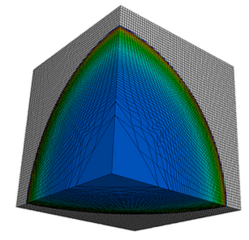
\includegraphics[width=0.4\textwidth]{2_context_hpc/LULESH.png}
    \caption[Visual representation of LULESH results]{Visual representation of LULESH results\protect\footnotemark}
    \label{fig:2_context_hpc:LULESH}
\end{figure}

\footnotetext{Image from \url{https://asc.llnl.gov/codes/proxy-apps/lulesh}}

Livermore Unstructured Lagrangian Explicit Shock Hydrodynamics (LULESH) is a
very popular C++ proxy application that is commonly used to benchmark HPC
clusters~\cite{Karlin2013}. The underlying physics problem that it solves is a
specific instance of a hydrodynamics problem, more specifically a Sedov blast
wave problem, which studies the deformation of materials in 3D, as explained
in~\cite{Hornung2011}. A graphical representation of an example result is
displayed on Figure~\ref{fig:2_context_hpc:LULESH}. As this application is very
popular, implementations of LULESH exist for most parallel programming
frameworks and hardware.

LULESH mainly uses point-to-point operations for its communications, along with
more occasional Reduce and AllReduce calls. The execution flow of the
application depends on the numerical results from computation, which is why it
is difficult (if at all possible) to make a skeleton version of this
application. It also has a constraint on the number of processes that need to be
used to run it: because of the way work is distributed on the MPI ranks, the
total number of process must be the cube of an integer (so 1, 8, 27 are valid
numbers of ranks for example).

\subsubsection{Quicksilver}

\begin{figure}[!ht]
    \centering
    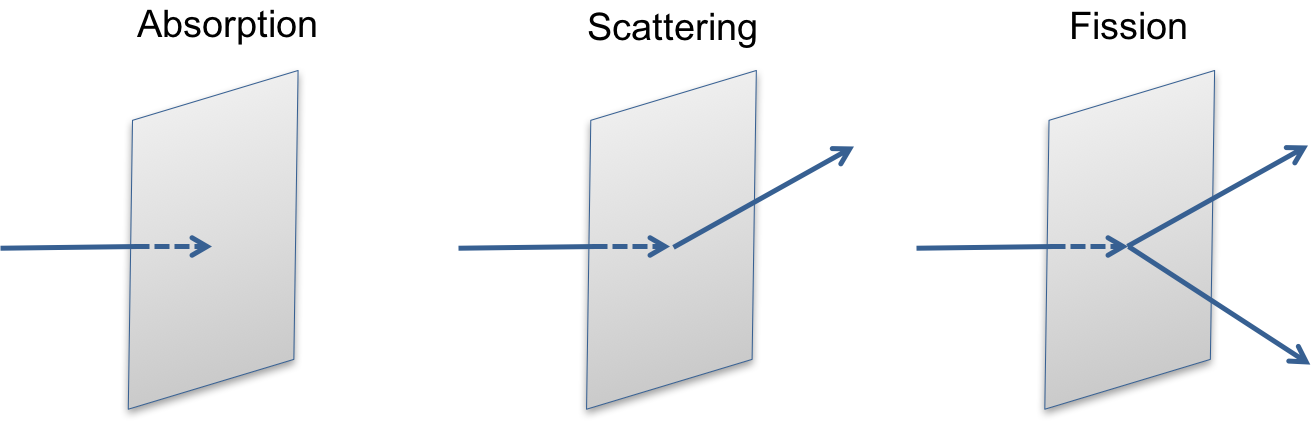
\includegraphics[width=0.6\textwidth]{2_context_hpc/Quicksilver.png}
    \caption[3 possible interactions that a particle can have in the Quicksilver model]{3 possible interactions that a particle can have in the Quicksilver model\protect\footnotemark}
    \label{fig:2_context_hpc:Quicksilver}
\end{figure}

\footnotetext{Image from \url{https://asc.llnl.gov/codes/proxy-apps/quicksilver}}

Quicksilver is a C++ proxy application that uses a Monte Carlo
algorithm~\cite{Carter1975} to solve a particle transport problem: it models a
configurable number of particles, and their interactions in 3 dimensions with a
predefined mesh. The possible interaction types are represented on
Figure~\ref{fig:2_context_hpc:Quicksilver}. Quicksilver has implementations both
on CPU, with OpenMP and MPI, and on GPU with CUDA.

It features a variety of point-to-point and collective operations, as well as
custom datatypes, which makes it an interesting app to study. However, similarly
to LULESH it is very hard to make a skeleton version for it as execution flow
depends on the correctness of calculations.

\subsubsection{HPL}

\begin{figure}[!ht]
    \centering
    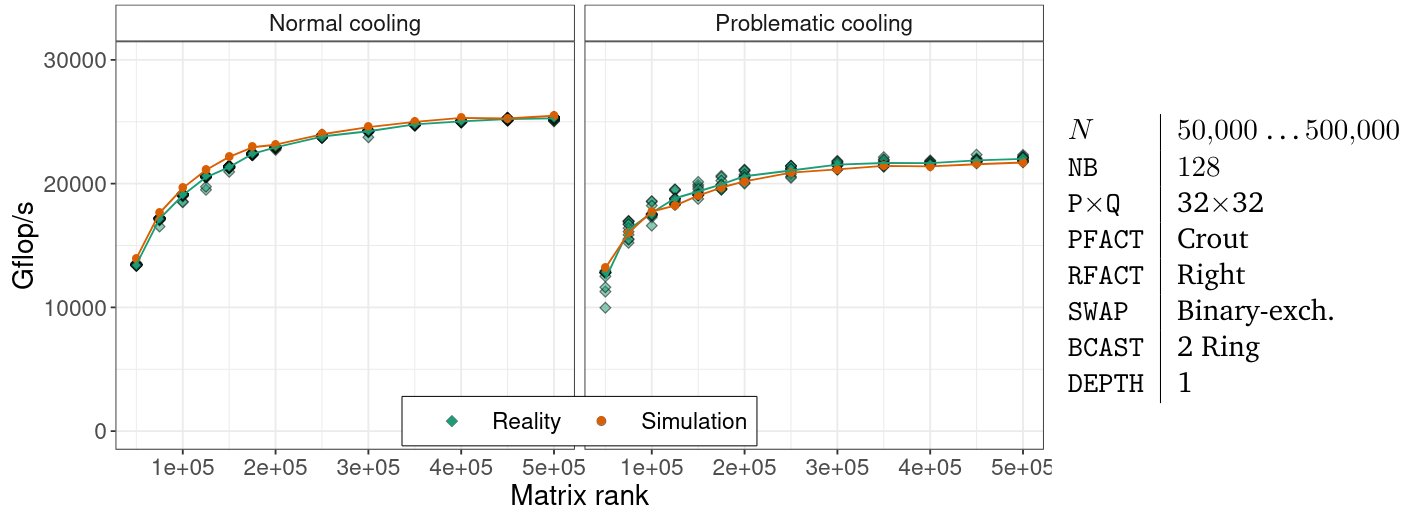
\includegraphics[width=1\textwidth]{2_context_hpc/HPL_Tom.png}
    \caption[Results of HPL simulation in SMPI in two scenarios]{Results of HPL
    simulation in SMPI in two scenarios. Image from~\cite{Cornebize2021}}
    \label{fig:2_context_hpc:HPL_Tom}
\end{figure}

High-Performance Linpack (HPL) is a very popular benchmark, famous for being
used to rank supercomputers in the Top500 list~\cite{Top500}. It solves a
mathematical problem, more specifically a randomly generated dense linear
system. The algorithm that is implemented is a lower-upper (LU) decomposition.

It relies on MPI for its communication, and on the Basic Linear Algebra
Subprograms (BLAS)~\cite{Lawson1979} for computation, which is a library that
has many implementations, some generic and some vendor specific. For example,
AMD provides its own version of BLIS~\cite{VanZee2015}, a framework that
provides a fast BLAS implementation, which is optimized for AMD CPUs (in
particular the Epyc and Ryzen architectures), and which is the version we will
use in our experiments.

HPL does not use any collective operation from MPI directly, instead the
application re-implements all collective primitives itself (using combinations
of point-to-point operations), and allows users to tune the algorithm used for
each type of operation in the input file that drives the execution.

What makes it an interesting application to study is that it has already been
the subject of many studies, and therefore it already has existing skeleton
versions: in this thesis we will be able to reuse a skeleton made for SMPI with
no modifications. Simulation results obtained with SMPI in two scenarios (with
or without a cooling incident on the cluster) are shown on
Figure~\ref{fig:2_context_hpc:HPL_Tom}. It also makes heavy use of user-made
datatypes and communicators (by splitting the global ``MPI\_COMM\_WORLD''),
which is not very common, so it is a good way to test these features in
simulation.


\chapter{Related work around simulation}
\label{chap:biblio_simu}

As discussed in the previous section, an HPC software stack can be complex, and
the hardware features many of optimizations and offloads that can have
unpredictable effect on the performance on real-life applications. Because of
this, it is very challenging to predict the execution time of an application on
a given cluster, although it is an important problem to solve, in order to
improve applications' code, optimize libraries, and design more performant
hardware for the next generation. It is also important to be able to model the
behavior of hardware before making physical prototypes, because it accelerates
the development and reduces the costs of hardware design by orders of magnitude.
For software developers, testing on real-life clusters, or hardware that is not
available yet, can be difficult and costly (since clusters require a huge amount
of power, and often have many users which need to share the resources). This is
why simulators are a crucial tool for both hardware designers and software
developers in HPC.

\section{Tradeoff between performance and accuracy}

We can categorize simulators in a few groups, depending on their use case: for
hardware designers, most of the time simulators need to be a faithful emulator
of real-world hardware, to be able to fine tune the behavior of the circuit to
get the desired output. This type of simulation is called Cycle Accurate, Bit
Accurate (CABA) when modeling processing units (like CPUs), and are often built
with frameworks like SystemC~\cite{Cornet2008} or gem5~\cite{Menard2017}
(sometimes both). When modeling networking hardware, this type of simulation is
called packet-level (or flit-level), and is typically built with frameworks such
as ns-3~\cite{Riley2010}, Omnet++~\cite{Varga2001} or CODES~\cite{Jain2017}. The
biggest advantage of this type of simulators is that they are very accurate and
faithful to real-world hardware, but the downside is they are often very
expensive to run in terms of performance, as the simulations are orders of
magnitude slower than real-world executions.

At the other side of the spectrum, analytical models use abstract heuristics to
estimate the execution time of an application, which allows users to get a rough
but very fast approximation of the performance of a program on a specific
cluster. The downside of these models is that to optimize performance they often
ignore some properties of the real-world hardware that can have an important
impact on the simulator's accuracy, such as congestion. In this category one of
the most popular network simulators is LogGOPSim~\cite{Hoefler2010}, which is
based on the LogP family of models. These models (LogP, LogGP and LogGPS) use
different numbers of parameters to get a more or less accurate estimation of
performance of network communications. They also need to be carefully
calibrated~\cite{Hoefler2007} in order to get any meaningful prediction, and
extended~\cite{Ferreira2018} to model high-level APIs such as MPI. For
computational estimations, the closest equivalent is the study of the complexity
of an algorithm~\cite{Cook1983,Turing1937}, which similarly does not give an
exact estimate of the performance to expect, but at least a good approximation
of the order of magnitude.

\section{Use cases and input formats}

Not only do simulators choose different tradeoffs between accuracy and
performance, but they also feature different methodologies, which translate into
different inputs. The two main types of models are offline simulators and online
simulators: while online simulators run the full application in a virtual world,
offline simulators only replay a trace file, given as an input.

Trace files used by offline simulators describe the computation and
communication phases of a given application, and they are obtained by
instrumenting an application (or library such as MPI) and running it on a
real-world cluster (ideally as similar as possible to the cluster the user wants
to model). This makes traces potentially difficult to obtain, and for large
applications the resulting file can be hard to handle because of its size.
Offline simulators then replay traces with different settings to model different
configurations (a faster network or a larger cluster for example). These
simulators include BigSim~\cite{Zheng2004}, Dimemas~\cite{Girona2000}, and
CODES~\cite{Cope2011}. While this methodology has a few downsides, it is still
very widely used, because it allows simulators to be very fast, and models which
are very abstract are often unable to run the full application anyway. This is
why analytical models tend to use this method, and some simulators which support
online simulation can have an option to generate or replay trace files (which is
the case of SMPI~\cite{Degomme2017a} for example). This approach is also
facilitated by the number of tools to analyze real world hardware's performance:
indeed, regardless of simulation, several studies~\cite{Jyothi2017} and tools
help analyze the performance of various workloads on a cluster, such as
Netgauge~\cite{Hoefler2007a}, Vampir~\cite{Knupfer2008},
Score-P~\cite{Knupfer2012}, or Autoperf~\cite{Chunduri2019}, most of which can
be used to obtain traces of an application's execution.

In the case of online simulators, the full application is given as an input,
with no prior real-world execution needed. With low-level models, the
application's binary can usually be run as-is on top of emulated hardware, and
function exactly as it would on real-world hardware. For more abstract models
(flow models for example), this is not always possible, and running the
application in simulation might require re-compiling it (which is what SMPI
does), or at least intercepting function calls that are implemented by the
simulator using \inline{LD_PRELOAD} or syscall interception for example. These
techniques were compared in more detail in~\cite{Bessad2015}, and syscall
interception was implemented in a tool called Simterpose. In our work, we will
implement the method chosen by SMPI, which intercepts communication primitives
using \inline{#define} macros in C/C++, and requires re-compiling the
application with specific flags. While this means that closed-source
applications cannot be simulated with this methodology, we will see in
Chapter~\ref{chap:low_level} that re-compilation offers many other advantages
which make this downside a small price to pay (especially since most commonly
used benchmarks are open-source).

\section{A few notable simulators}

While we chose to use SimGrid for this thesis, which will be described in detail
in the next section, there are several other projects with similar goals that
could have been used. This section will present SST and Shadow in particular,
which are also commonly used for this type of work.

\subsection{Structural Simulation Toolkit}

The Structural Simulation Toolkit (SST)~\cite{Hendry}, developed by Sandia
National Laboratories, is a very popular choice when picking a simulation
framework, for both offline and online simulation. It is divided into two major
components: the SST core, and SST/Macro. The core~\cite{Rodrigues2011}
implements the startup and configuration management required by the simulator;
it is designed as a modular architecture, where models can then be plugged
(using an XML configuration file). SST/Macro~\cite{Curtis2010} is an extensible
Parallel Discrete Event Simulator (PDES) implemented on top of MPI. It exposes
several network models, including analytical and packet-level ones.
Unfortunately flow models are no longer supported, in order to focus on the
other two types of models. This is the main reason why we chose to use SimGrid
instead. SST provides many low-level models~\cite{Murphy2004} for commonly used
components, such as CPUs, DRAM, memory controllers, simplistic NICs, etc. which
makes it a good tool to run unmodified binaries on top of detailed hardware
models, but this has an important cost in terms of performance. SST also
supports the modeling of other properties of a cluster than the simulated time,
as it integrates models of power consumption and
temperature~\cite{Hsieh2012}.

While SST has been used to model Portals 4 hardware
before~\cite{DiGirolamo2019}, this type of model is lower-level than what we
intend to build in this thesis. This particular work is also unfortunately not
open-source, which made it impossible to reuse, but the results show that SST is
also a viable option for the co-design of HPC networking hardware. 

\subsection{Shadow}

Shadow is a parallel discrete event network simulator. While it was originally
made specifically to study the TOR network specifically~\cite{Jansen2012}, it
has since demonstrated good results when modeling diverse applications, such as
P2P networks~\cite{Jansen2022}. We did not use it in this thesis, because it is
still mainly an IP simulator, which is not widely known in the HPC community. It
is still an interesting project because it tackles many issues that also arise
in the type of HPC simulators that we will present in our work, and as such it
is a good source of inspiration in many cases. In particular, Shadow executes
unmodified applications, hooking into their code with a mixture of library
preloading (using the \inline{LD_PRELOAD} environment variable on Linux) and
syscall interception. Then the simulator emulates a Linux kernel in order to
make syscall interception transparent to the application, which involves
reimplementing all logic that uses time, the filesystem, and the network (at TCP
and UDP level). They also re-implement all features related to random generation
(such as the content of the \inline{/dev/random} file) in order to make
simulations deterministic and easily reproducible. While this strategy is very
efficient for Shadow's use cases, in our work we do not need to go as far as
intercepting system calls. The reason is that in HPC, networking hardware uses
OS bypass to optimize the performance of applications, and therefore software
libraries operate mostly in user space, with little system calls.

\section{SimGrid}
\label{sec:3_related_work_simu:simgrid}

We chose SimGrid to build our simulator because of its performant flow model and
flexibility. SimGrid was first introduced in 2001 as ``a simulation toolkit for
the study of scheduling algorithms for distributed
application''~\cite{Casanova2001a}, but it has since evolved to become a
versatile simulation framework, with applications intended to cover ``the
cluster, grid, peer-to-peer, volunteer, or cloud computing domain''
(\cite{Casanova2014a}). While this goal seems ambitious (since many of these
domains already have very specific simulators), many studies have shown that
SimGrid is indeed a good fit for many of these use-cases. To name only a few, we
can find existing work on domains as varied as HPL
simulation~\cite{Cornebize2017b,Cornebize2017a,Cornebize2021} using the SMPI
simulator, TCP networks~\cite{Bedaride2013a} by leveraging a TCP-specific
network model that was added to SimGrid in 2009~\cite{Velho2009a}, Workflow
Management Systems~\cite{Casanova2019}, and even P2P networks with millions of
simulated machines~\cite{Quinson2013}.

\subsection{Architecture}

\begin{figure}[!ht]
    \centering
    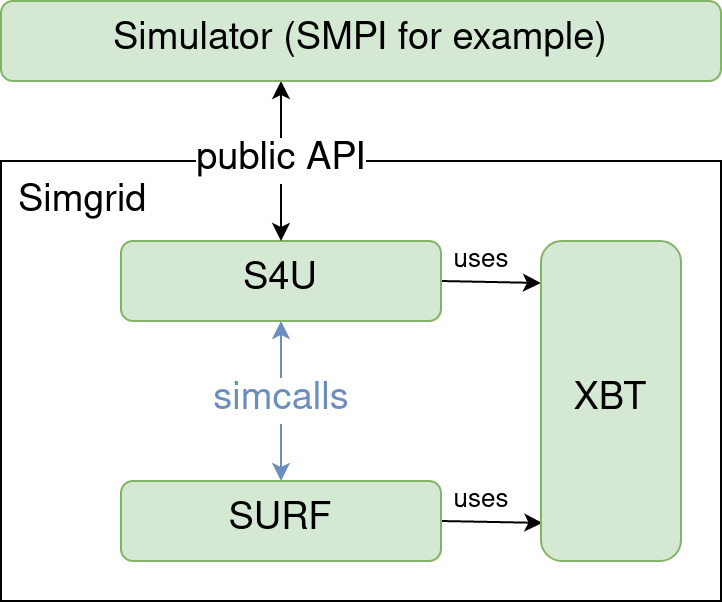
\includegraphics[width=0.5\textwidth]{3_related_work_simu/simgrid_arch.jpg}
    \caption{SimGrid's architecture}
    \label{fig:3_related_work_simu:SimGrid_arch}
\end{figure}

Internally, SimGrid is made of three layers (as seen in
Figure~\ref{fig:3_related_work_simu:SimGrid_arch}): at the lowest level, XBT
(eXtended Bundle of Tools) is a collection of optimized C function to manipulate
data structures, timers and other utilities. On top of it, the simulation kernel
(called SURF) manages the virtual time and resources: it is in this layer that
the duration of Activities (network, IO or compute) is computed in order to
progress the virtual time and schedule the next piece of user code to be
executed. The highest level is called S4U (Simgrid For You) and it implements
the ``public'' API that is exposed to users. It provides abstractions for
low-level concepts using C++ classes, representing the various resources that
user code can interact with: Hosts represent simulated pieces of hardware (like
a full machine, or a part of a machine) and Links represent any cable (usually
network cables) that connects Hosts. Additionally, S4U provides classes to
better abstract user code and communication, namely Actors and Mailboxes. Actors
represent any piece of code that is to be scheduled asynchronously from other
Actors' code, in other terms it will often model a process in the simulated
world (or some hardware's logic that runs independently of other hardware).
Actors need to be instantiated on a specific Host in the simulated platform in
order for SURF to know at which speed computation phases need to be executed.
Mailboxes on the other hand, are a mechanism that allows Actors to communicate:
traditionally, in SimGrid, data transfers will occur when two Actors issue a
``send'' and a ``receive'' call to the same Mailbox (which are identified by a
unique name). By default, Mailboxes are not linked to a specific Host (they are
not ``located'' anywhere on the simulated platform), which means that the Links
used in a communication can only be decided when both the sender and the
receiver have issued their call (\inline{put} to send or \inline{get} to
receive) to the Mailbox. Indeed, this is only at this instant that SURF will be
able to determine which Hosts are communicating. This means that Mailboxes
effectively work as ``rendezvous'' points, although it is possible to set a
specific Actor as a ``permanent receiver'' for a Mailbox, which allows the
transfer to start at soon as a ``send'' is issued on the Mailbox (before any
``receive''). This mechanic is depicted in
Figure~\ref{fig:3_related_work_simu:SimGrid_mailboxes}, and it will be used
extensively in our simulator, which will be described in more detail in
Chapter~\ref{chap:low_level}.

\begin{figure}[!ht]
    \centering
    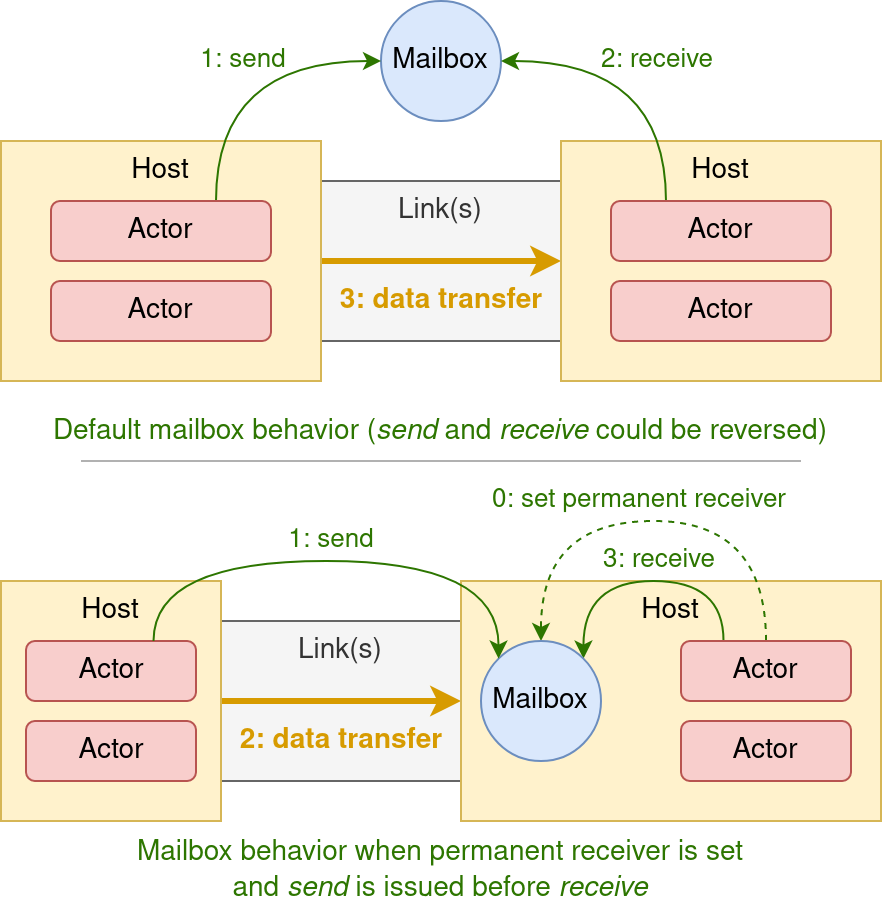
\includegraphics[width=0.7\textwidth]{3_related_work_simu/simgrid_mailboxes.png}
    \caption{SimGrid's mailbox system}
    \label{fig:3_related_work_simu:SimGrid_mailboxes}
\end{figure}

SimGrid uses cooperative actors, and it is architectured in a way that is heavily
inspired by operating systems: indeed, the user-space interface (S4U)
communicates with the simulation kernel (SURF) using a mechanism called
``simcalls'', which are very similar to syscalls on Linux. A simcall is issued
by an Actor each time it needs to perform an operation that might impact the
simulated time (any computation, communication or IO). Effectively simcalls are
a way for Actors to ask SURF to perform the desired operation and wake them up
again either at the same date in the simulated world (in case of asynchronous
operations), or whenever the operation is completed (in the case of synchronous
operation), so each time an Actor performs a simcall it will yield to the kernel
and trigger a new scheduling round. This only happens when Actors perform
simcall, as SimGrid simulations are cooperative, therefore it is the
responsibility of Actors to yield (either using a simcall or by calling a
dedicated primitive to do it explicitly).

\subsection{Usage}

While SimGrid is programmed with C++ 17, it offers bindings in C++ and Python. A
Java interface also used to exist for the old MSG user API, but it has not been
maintained when MSG was deprecated in favor of the S4U interface. During this
thesis we use exclusively the C++ S4U interface. An example of a toy simulation
using this interface is shown on
Figure~\ref{fig:3_related_work_simu:SimGrid_pingpong}.

\begin{figure}[!ht]
    \lstinputlisting[basicstyle=\ttfamily\scriptsize,frame=bt,language=C++]{3_related_work_simu/simgrid_pingpong.cpp}
    \caption{Simplistic ping-pong with SimGrid's S4U interface}
    \label{fig:3_related_work_simu:SimGrid_pingpong}
\end{figure}

In this example, which implements a ping-pong with exponential message sizes,
first our two Actor types are defined: \inline{initiator} to start the
``pings'', and \inline{target} which will receive them and send ``pongs'' back.
Their behaviors are simply a function, because that is sufficient for this
simple example, but SimGrid supports making Actors from anything that is
callable in C++, including objects (by overloading the \inline{()} operator,
which we will use extensively in this thesis). The initiator Actor simply sends
``pings'' of increasing size, attaching a sequence number to each message
(\inline{iteration}), and waits for ``pongs'', checking that the ``pong''
sequence number is the same that was sent. The target ``daemonizes'' itself,
which means that the simulation will end (and this Actor will be killed
automatically) when all the other Actors are done executing their logic (which
means that the end of the initiator will trigger the end of the simulation in
this case). While this example is very simple, it already shows a few
interesting things about SimGrid: First, we can see how the XBT layer can be
used for several utility purposes, like an assertion API and a logging system.
This logging system is very complete, and is used through C-style macros that
mimic the \inline{printf} API. Even though that is not showcased in this
simplistic example, it supports a tree-like structure of categories and
subcategories, which enables fine-tuning on the command line which level of log
to display for each category. In the Actors' code we can see the S4U API being
used to interact with the Mailbox system in order to send and receive messages.
As most resources in SimGrid, Mailboxes follow the RAII paradigm (Resource
Acquisition Is Initialization), therefore we do not have to instantiate the
Mailbox ourselves, we simply ask SimGrid to give us a Mailbox with that name,
and internally S4U will either return it to us if it already exists or create it
if it does not. This means that in our example, we do not know if the two
mailboxes are going to be created from the \inline{s4u::Mailbox::by_name} calls
from initiator or the target (since all this code happens at $t = 0$ in the
simulated world), but it does not matter since the result is going to be
identical. It is worth noting that even if we managed to cause a potential race
condition (because of two Actors executing code at the same simulated time), it
is easier to debug in simulation compared to a real-world execution, because
even though the order of operation happening at the same simulated time is
random from a user perspective, it is deterministic, to ensure the
reproducibility of SimGrid's simulation. Finally, the \inline{main} function
sets up the simulation, declaring our Actors, and loading the platform and
deployment from XML files before starting the simulation Engine. The output of
this toy simulation is displayed on
Figure~\ref{fig:3_related_work_simu:Pingpong_output}. We can see that even
though SimGrid provides methods to get the simulated time, we did not need to
use them, as the logging system from XBT already prints the current Actor,
simulated time, category and log level on each line.

\begin{figure}[!t]
    \lstinputlisting[basicstyle=\ttfamily\scriptsize,frame=bt]{3_related_work_simu/pingpong_output.txt}
    \caption{Ping-pong's output}
    \label{fig:3_related_work_simu:Pingpong_output}
\end{figure}

\subsection{Performance and isolation concerns}

Despite being used to build single-threaded simulators, SimGrid has demonstrated
a very good scalability thanks in particular to its platform
representation~\cite{Bobelin2012} and the optimization of its sequential
Discrete Event Simulation (DES) kernel~\cite{Degomme2017a}. This is because a
DES requires many synchronizations, since there is a central value of the
current simulated time that is shared by all Actors in the system, making
parallelism very difficult. Some simulation frameworks try to use several
threads regardless, or to work on top of MPI to distribute work on several
machines (which is the case of the SST for example). The approach used varies,
for example ROSS~\cite{Carothers2002} uses an optimistic scheduler to reduce the
number of synchronizations required to the minimum, but this means that
backtracking might be required when an inconsistency is detected. This makes
simulators harder to write (since they need to implement rollback mechanisms),
and it also limits the speedup that can be obtained from parallelization. Having
a sequential DES also makes writing a simulator significantly easier: race
conditions can still happen due to the asynchronous nature of the simulation,
but most data structures can be used safely with no synchronization since Actors
are executed one at a time, and therefore cannot access a piece of data at the
same wallclock time.

The biggest issue that arises from having a single-threaded simulator is that
all Actors share the same memory space. To work around this issue, and have a
dedicated stack for each Actor, SimGrid allocates a tunable amount of memory to
each Actor's stack, and when switching context from one Actor to the other it
provides different mechanisms: either using a full thread for each Actor, but
with only one running at any given time (which is a very portable solution but
very slow), \inline{ucontext} from the System V API (which are faster but
available only on Linux and FreeBSD), boost contexts (which are also reasonably
fast but add a dependency), and finally ``raw'' contexts, which are implemented
by SimGrid directly in x86 and amd64 assembly code. This last solution is
extremely fast, as it requires only a few CPU cycles to switch contexts. Its
only two downsides are that it is not portable to other CPU architectures, and
that this way of moving registers manually can make debugging much harder (in
tools like GDB for example). For this reason, in this thesis we use ``thread''
context when debugging is needed (as it is very compatible with standard tools),
and ``raw'' contexts when making full scale experiments.

To describe the simulated platform, on which Actors will be instantiated,
SimGrid provides several interfaces. The most common one is through a static XML
file, which is a list of Hosts, Links, and Routes to describe which Links are
used to communicate between two Hosts. Additionally, some extra tags allow a
more concise description of the platform, such as Router or Cluster to describe
common topologies, but they are simply syntactic sugar and do not add any
feature. This simulated hardware can also be grouped in NetZones that help
describing heterogeneous platforms. Because a static platform can be very
verbose (and the parsing of XML can have an important negative impact on
performance for large platforms), SimGrid also exposes a programmatic API, which
helps describe regular topologies with loops for example. At the beginning of
this thesis this API used to be simplistic and required users to describe their
platform in Lua, but it has since been deprecated in favor of a C++ API that is
much more powerful. Although we started by using SimGrid with the XML
description, we switched to the C++ API when it became available, therefore all
our experiments will use this interface.

Finally, SimGrid offers a system of Plugins, which allows users to listen to
events and extend the features natively offered by the framework. The most
popular are the Energy and Filesystem plugins, which allow users to respectively
estimate the power consumption of hardware, and model a complete Filesystem on
top of the basic Storage features natively offered by SimGrid. We did not use
the plugin system intensively in this thesis.

\section{High-level models}

While some specific parts of MPI have been studied in depth, such as the
matching engine~\cite{Levy2019}, it is very hard to fully model a complete MPI
implementation In HPC, there are two traditional approaches to model high-level
APIs, such as MPI or OpenSHMEM for example. The offline approach requires
obtaining a trace of the communications from a real-world execution, and then
replaying it in simulation, potentially with different parameters, as we
presented earlier. Such studies allow very fast simulation but require users to
be able to obtain a realistic trace in the first place, which can be
problematic. The online approach usually involves re-implementing the whole API
on top of a simulation framework, in order to intercept communication primitives
during the runtime of the application. While this requires a lot of work, it is
the most commonly used, for example by SMPI~\cite{Degomme2017a},
xSim~\cite{Bohm2011} or SST/Macro~\cite{Hendry}, which all provide a complete
MPI implementation in simulation (SMPI even goes as far as implementing several
algorithms for each operation to mimic different real-word implementations of
the MPI standard). Another approach would be to run a real-world API on top of a
simulated low-level network library. While this makes the development of the
simulator easier (since low-level libraries are usually more simplistic than
high-level APIs), it proves very difficult to provide a simulated environment
that is realistic enough to run the high-level API unmodified, which is why this
approach is seldom used. We found an example of it in~\cite{Knight2018}, which
manages to run the GASNet runtime on top of a simulated uGNI implementation
(based on SST), although running more common APIs such as OpenMPI are left as
future work. This last approach will be implemented for OpenMPI and OpenSHMEM
over a simulated Portals implementation (using SimGrid) in this thesis, using
different technical solutions than~\cite{Knight2018} to overcome the challenges
that arise in the process (and which are described in detail in
Chapter~\ref{chap:high_level}).

\section{Multi-level modeling}

Because the performance / accuracy tradeoff of simulators is their biggest
limitation, some studies have tried to make it more dynamic. For example,
Behavioral Emulation~\cite{Ramaswamy2018} tries to add this type of feature to
the SST, by allowing users to write models of various granularity for each type
of hardware. While this is an interesting project, it is very costly to use in
terms of development time, because it is the responsibility of users to write
each model at each granularity that they wish to study. Some simulators also
feature options to make their low-level faster at the cost of some accuracy, for
example by ignoring very short events, but from our experiments this type of
configuration usually has a limited impact on performance and accuracy, as the
underlying model is mostly the same in the end.


\chapter{S4BXI, a low-level Portals model}
\label{chap:low_level}

The goal of this thesis is to model applications that rely on the Portals API
for their network transport. Although these applications are written using
high-level communication libraries, we also want to take model low-level
properties of the BXI hardware. This leads us to design a simulator that is
abstract enough to be able to scale to hundreds of simulated processes, but
which also features a model of the BXI NIC that is realistic enough to model the
most significant optimizations of the hardware.

This chapter presents the simulator that we designed, S4BXI by focusing on the
low-level model, whereas Chapter~\ref{chap:high_level} will give more details on
how it integrates with high-level APIs such as MPI. S4BXI is based on SimGrid,
and as such it is a Discrete Event Simulator (DES) based on a cooperative actor
model. It models the Portals~4 API, and as such it is by design a good model for
BXI NICs, which implement this API in hardware. It is made in C/C++ from around
9 thousand lines of code\footnote{Counted using cloc:
\url{https://github.com/AlDanial/cloc}}. Finally, it is open-source under LGPLv2
license, and all the relevant links (source code, publications, related tools,
etc.) can be found at \url{https://s4bxi.julien-emmanuel.com}.

We will start by describing how the real-world hardware is
modeled using SimGrid's platform, as well as how we instantiate Actors on this
platform, and then we will detail some technical aspects of our Portals
implementation. Finally, we will present some validation experiments at a low
level before moving on to higher-level experiments in the next chapter.

\section{Platform model}

As introduced in Chapter~\ref{chap:biblio_simu}, SimGrid platforms are composed
of Hosts, that represent simulated hardware, and Links, which represent cables
(or buses). SimGrid allows any combination of Hosts and Links, but for the
purpose of our simulators we add a few constraints on this representation.

\subsubsection{Host types} 

In SimGrid, Hosts are supposed to be able to represent whole machines, and
SimGrid natively allows to configure a Host as multicore (a virtual Host in the
model can have several virtual cores). SimGrid does not have a fine model of
scheduler inside each Host, and it does not model each core independently, which
means that in practice, in the case of a multicore Host, every computation phase
is evenly distributed across all cores.

In our case this proved to be problematic, as we wanted to be able to assign
specific tasks to specific (virtual) cores, instead of having each computation
phase distributed across all cores. For this reason, in S4BXI we use Hosts not
to model full machines, but instead we define two types of Hosts, which
represent hardware at a finer granularity: we have Hosts that represent a single
CPU core, and Hosts that represent a NIC. This means that in practice, in our
model each physical machine is represented by $N + 1$ virtual Hosts, where $N$
is the number of cores in the CPU.

\subsubsection{Link types} To connect these Hosts together, we have two types of
Links: PCI Links and BXI Links. PCI Links model the PCIe bus inside each
machine, which connects the NIC to the rest of the machine. This link is
important because it is typically not modeled by other flow-level simulators, in
particular SMPI, which usually models a whole machine with a single Host. We
decided to do it because as interconnection networks get faster and faster, the
transfer times across the PCI bus is of the same order of magnitude as network
transfer times, which means that congestion on the PCI bus can happen and have
an impact on the speed of inter-node communications. The second type of Links is
the more traditional network cables that connect NICs to switches, and switches
together.

\begin{figure}[!ht]
    \centering
    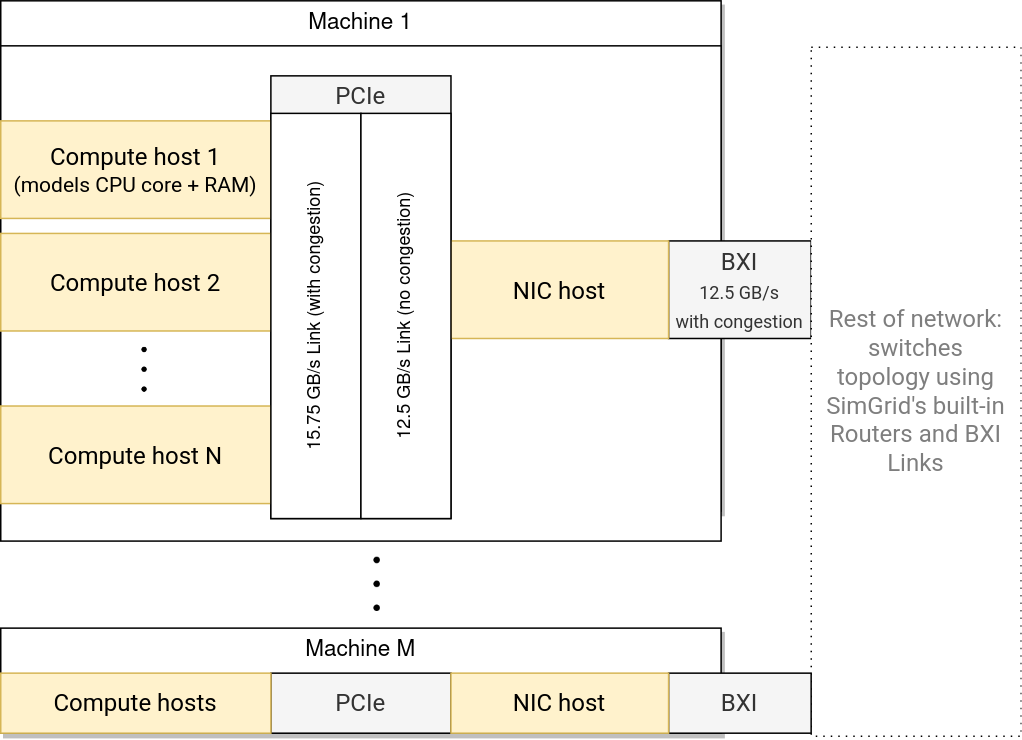
\includegraphics[width=0.8\textwidth]{4_portals/hosts_links.png}
    \caption{Platform model in S4BXI}
    \label{fig:4_portals:Hosts_Links}
\end{figure}

One of the difficulties resides in the model of the PCI bus: while third
generation PCIe x16 networks have a maximum theoretical bandwidth of 15.75 GB/s,
most of our transfers (especially the transfers of consequent size) are going to
flow from the PCI bus directly onto the BXI cable (which has a maximum bandwidth
of 12.5 GB/s), with minimal processing in the middle. In real life this is
handled with packetisation on each side of the NIC (across the PCI bus and then
across the BXI cable), but because we use a flow model that operates at
message-level, we cannot implement this level of granularity without losing a lot
of performance. While we cannot model a total maximum bandwidth of 15.75 GB/s and
a per-message bandwidth of 12.5 GB/s in a single Link in SimGrid, we can model
this behavior using two Links that each transfer has to go through: a 12.5 GB/s
Link on which congestion is not considered, which limits the speed of each
individual transfer, and a 15.75 GB/s Link on which congestion is considered,
which limits the speed of all simultaneous transfers across the bus at any given
time. We are allowed to connect these two Links back to back in simulation, even
though it does not correspond to what can be done in real life. Indeed, SimGrid
is very permissive in the description of platforms: every Host and Link has a
Netpoint (in SimGrid vocabulary), which can be connected to any other Netpoint
regardless of the type of hardware it is bound to, so it effectively allows
users to connect Links together.

It is worth noting that there is no particular model for switches: indeed, we
use native Router components provided by SimGrid to represent BXI switches, but
even these components are just syntactic sugar to represent a Host with no
Actors. These Routers work even though they do not implement any behavior,
because the routing logic across the cluster (i.e. the set of Links to be used
when communicating between two Hosts) is not performed at a high-level by
Actors, but it is implemented at a low-level in the SURF layer of SimGrid. While
making a more detailed model of switches at S4U-level using Actors would be an
interesting subject of study, we chose to use the defaults routing algorithms
offered by SimGrid in SURF because their fat-tree routing is faithful enough to
what happens in real-world BXI fat-trees for our needs.

The platform model that results from our Links and Hosts is depicted on
Figure~\ref{fig:4_portals:Hosts_Links}, with a focus on one machine composed of
$N$ CPU cores.

\section{Actor placement}

Along with the platform description, a simulation needs to know which Actors to
deploy on the simulated Hosts, which is done through a ``deployment'' in
SimGrid. Similarly to the platform description, this can be done either
statically in XML or dynamically in C++. Throughout this thesis we used a static
XML deployment, since it is more concise than platform files, and therefore does
not suffer the same performance issues (even though in some situations S4BXI may
spawn a short-lived Actor to delay a specific task). Since the different types
of Actors to be deployed are the same in each simulation, and only numerical
parameters change (number of process to be deployed, number of nodes to be used,
etc.), we made tools to automate the process of generating deployment
files\footnote{\url{https://framagit.org/s4bxi/s4bxi-config-generator}}.

In order to implement the Portals API on top of the simulated hardware described
earlier, S4BXI provides several types of Actors, each of which correspond to a
different part of the communication logic. Their placement is represented on
Figure~\ref{fig:4_portals:actor_placement} and will be detailed in the next
sections.

\begin{figure}[!ht]
    \centering
    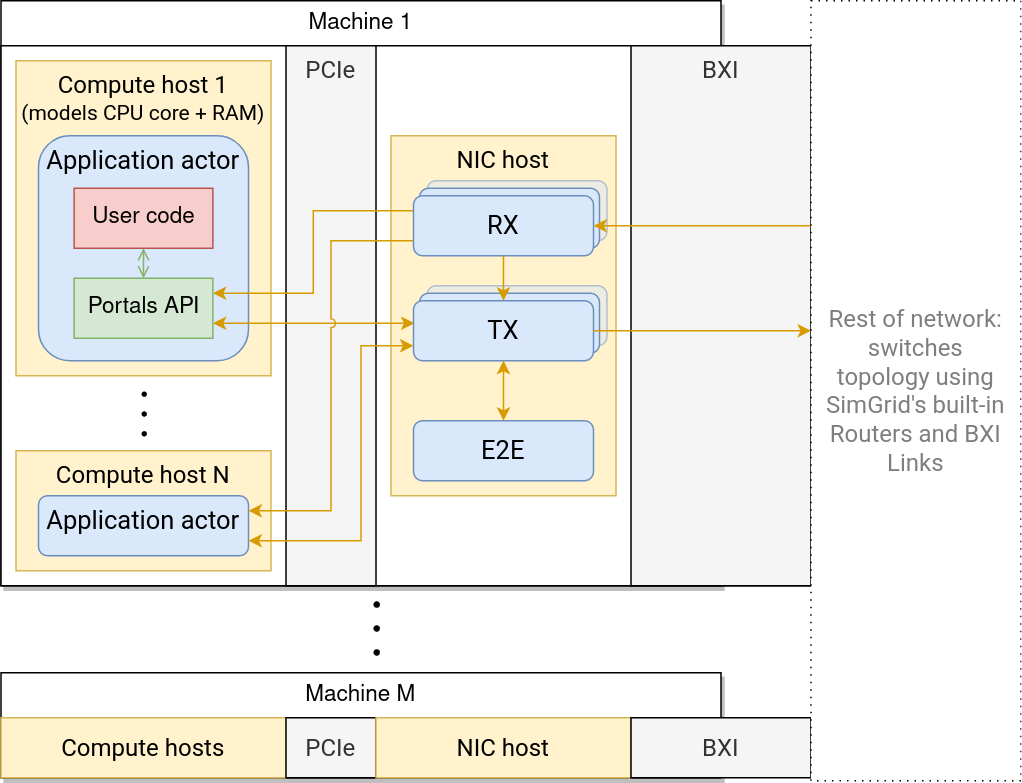
\includegraphics[width=0.8\textwidth]{4_portals/actor_placement.png}
    \caption{Actor placement in S4BXI}
    \label{fig:4_portals:actor_placement}
\end{figure}

\subsection{On-NIC Actors}

Since the Portals API is implemented in hardware by the BXI NIC, most of the
Portals implementation is done through three types of Actors that are
instantiated on the ``NIC Host'' of each machine in our platform:

\subsubsection{TX Actor}

TX Actors model the ``transmission'' logic of the NIC. This means listening to
command queues, processing message requests by doing any Direct Memory Access
(DMA) and generating any event that might be required, and finally sending
messages on the BXI Link to the rest of the network (through SimGrid's Mailbox
system). While the simulation works with only one TX Actor per NIC, users of
S4BXI can choose to instantiate several, either to model parallel processing
capabilities of the NIC, or to model different types of traffic. In BXI this
last feature corresponds to the Virtual Networks that were presented in
Section~\ref{subsubsec:2_context_hpc:VNs}.

\subsubsection{RX Actor}
\label{subsubsec:4_portals:RX}

RX Actors model the ``receive'' logic of the NIC. To do this they listen to
SimGrid Mailboxes, of which they are the permanent receiver (so that incoming
messages can keep flowing in even if no Actor is available to process them yet,
as described in Section~\ref{sec:3_related_work_simu:simgrid}). Then these
actors process the request depending on its type, applying any Atomic operation,
etc., and finally if an ACK or a Response is to be sent back it will be
forwarded to the corresponding TX command queue (either \textit{compute} or
\textit{service}). Similarly to TX Actors, RX Actors can be instantiated several
times to model different VNs, or parallel processing capabilities of the
hardware. For example, BXI NICs typically have four independent
Application-Specific Instruction set Processors (ASIP) for this purpose, which
are called List Management Engines (LME).

\subsubsection{E2E Actor}

E2E Actors model the End-to-End reliability logic of the NIC which was described
in Section~\ref{subsubsec:2_context_hpc:E2E}. Since our simulator implements a
flow model at message-level, it cannot model the CRC processing (encoding at
sender, verification at receiver), since it is performed on each packet, but it
models completely the timeout mechanism that is implemented in BXI, to
retransmit messages which did not get acknowledged on time. The parameters
(number of retransmissions and delay before retransmitting) are tunable using
environment variables (\inline{S4BXI_MAX_RETRIES} and
\inline{RETRY_TIMEOUT} respectively). In S4BXI, the E2E Actor of each machine
receives a copy of each message that is issued by TX. The only exception is for
BXI ACKs: in order not to have an infinite loop of acknowledgements (similar to
the Two Generals'
Problem\footnote{\url{https://en.wikipedia.org/wiki/Two_Generals_Problem}}),
these messages cannot have a further level of ACK, and they are therefore
delivered unreliably. For each message, the E2E Actor then sleeps until the
delay for retransmission is met. It then checks if an RX Actor has marked the
message as ``acknowledged'' or not, and either drops the message if it is the
case, or sends it back to the TX command queue for retransmission if the message
seems to have been lost. This logic is represented on
Figure~\ref{fig:4_portals:e2e_logic}: in this example only the first message
sent is acknowledged in time, so the second one needs to be retransmitted.

\begin{figure}[!ht]
    \centering
    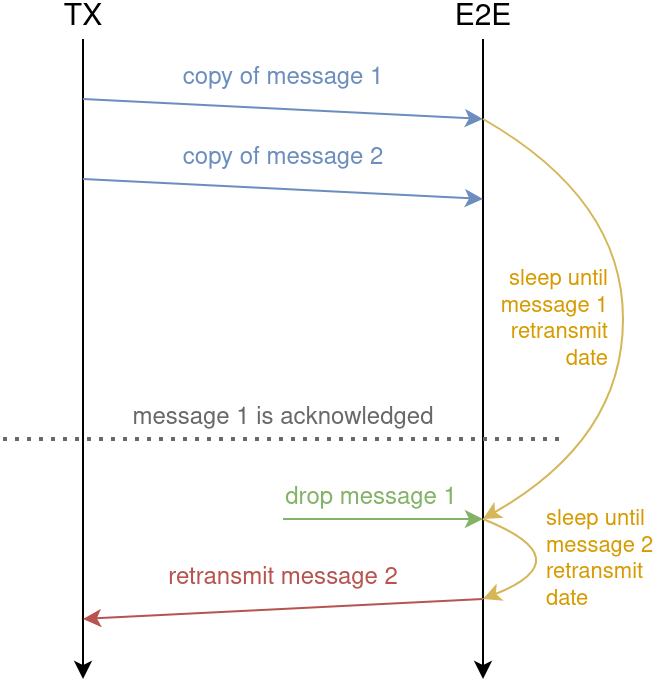
\includegraphics[width=0.6\textwidth]{4_portals/E2E_seq.png}
    \caption{E2E logic in S4BXI}
    \label{fig:4_portals:e2e_logic}
\end{figure}

It is important to note that although several RX and TX Actors can be
instantiated, every machine only requires one E2E Actor. This is because the
delay before retransmitting a message is constant in BXI (as it is a parameter
of the BXI kernel module), and therefore if messages need to be retransmitted it
will always be in the same order that they are received in by the E2E Actor.
This means that this Actor can safely sleep until the next retransmission date
when it processes a message, because even if another one is created in the
meantime its retransmission date will necessarily occur later. Additionally, we
can use a single ``First In, First Out'' (FIFO) data structure for all
communications between TX Actors and the E2E Actors (in which TX Actors writes
messages, which are read by the E2E Actor).

\subsection{Actors on CPU cores}
\label{subsec:4_portals:UserAppActors}

While the Actors instantiated on the NIC have a fixed behavior, Actors deployed
on the simulated CPU cores must be more flexible in order to model any user
application (as long as it uses the Portals API as its communication layer of
course). This is done in a way that is strongly inspired by SMPI: S4BXI requires
the user application to be compiled as a shared library, which allows the
simulator to use the \inline{dlopen} and \inline{dlsym} C functions to
load the \inline{main} function from the program and run it in simulation.
Since SimGrid uses cooperatives Actors, the user application simply yields
automatically when any network operation is performed, through the Portals API
which links with the implementation in S4BXI instead of a real-world one.

\section{Portals model}

\subsection{Representation in S4BXI}

In S4BXI, data exchanges are modeled using different Mailboxes, depicted in
Figure~\ref{fig:4_portals:s4bxi_mailboxes}. We can see that the event system
translates to a variable number of mailboxes (one for each EQ) that are created
through allocations by the user code (\inline{PtEQAlloc} for EQs for example),
and can then be queried through the Portals API. The mailboxes on the NIC do not
directly map to Portals data structure, instead they are an approximate model of
the hardware pipeline inside BXI NICs. We did not go for a faithful
representation here, because the real-word components of the NIC are very
complex, feature many more queues, and manipulate data at a different
granularity in different places (for example packet size on the network is 72
bytes, while transfers across a PCI bus can range between 128 and 4096 bytes of
packet size), whereas our simulator models traffic at message level, and
therefore is not suited to model individual packets in the NIC. This design
costs some accuracy, but greatly improves the performance of S4BXI.

In our model, TX Actors share \portalsAbbr{Commands Queues}{CQ}, one for each
Virtual Network that is used by the simulation's deployment (since inside each
VN operations must be strictly ordered according to the Portals's
specification). They wait for commands from other Actors in an infinite loop and
process them sequentially. These command queues are not directly Mailboxes: we
added a layer of abstraction on top of it that we will call ``S4BXI Queue''.
These queues mimic the Mailbox interface, but they provide two implementations:
they can either simply map to a Mailbox internally, or use a more performant
implementation based on a C++ \inline{std::queue} to store entries and a
\inline{simgrid::s4u::Semaphore} to allow processes to wait for a piece of data
to be available (a standard C++ semaphore cannot be used because it needs to be
blocking in the simulated world). This allows our queues to either model the
time it takes to transfer data to them (using the Mailbox system), or to make
operations instantaneous, which is often less accurate but will slightly improve
the performance of the simulator. Similarly, RX Actors also poll on Mailboxes,
one per VN, but which contain the incoming messages from the network. These
Actors implement the processing of these messages, including the matching logic
of MEs, any memory operation that might be required, and if a response is
needed, it is created in the RX Actor and forwarded to TX Actors through the
corresponding S4BXI Queue. Finally, the E2E Actor has its own S4BXI Queue, which
receives a copy of each message that TX Actors send on the network, except for
BXI ACKs which do not have their own acknowledgement.

\begin{figure}[!ht]
    \centering
    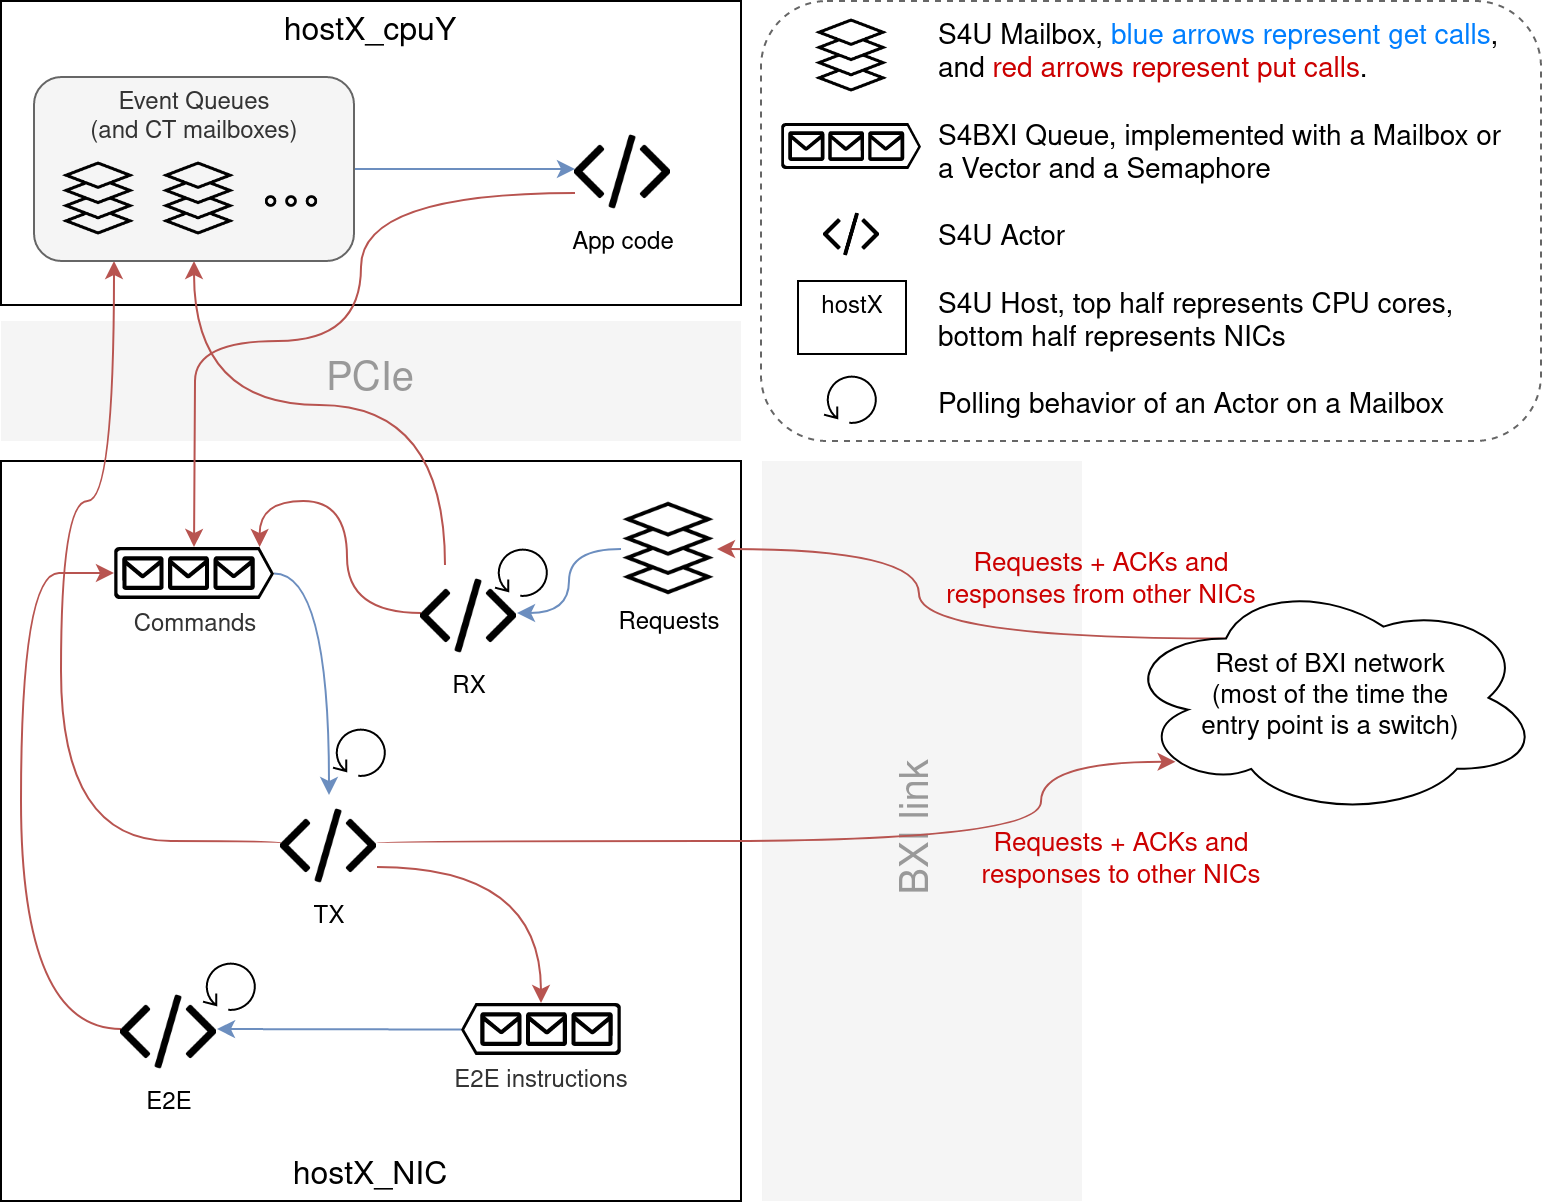
\includegraphics[width=1\textwidth]{4_portals/s4bxi_mailboxes.png}
    \caption{Mailboxe usage in S4BXI}
    \label{fig:4_portals:s4bxi_mailboxes}
\end{figure}

\subsection{Tuning for the BXI interconnect}

While Portals is a good specification for the API that should be exposed to
users, at the lowest level significant freedom is left to the implementation.
This results in many low-level design choices that need to be made in order to
run this API on real-world hardware. Several of these characteristics cannot be
modeled directly in S4BXI, because they are implemented at flit-level in BXI
hardware. This is the case of low-level flow control for example, which is
achieved using a credit-based mechanism in the real-world hardware. In this
section we will present the specific properties of BXI which are modeled in
S4BXI, because they operate at a level of granularity that is coherent with our
flow model.

\subsubsection{Virtual Networks}

Virtual Networks in BXI were presented in
Section~\ref{subsubsec:2_context_hpc:VNs}. They are fully modeled in S4BXI, by
assigning a VN number (from zero to three) to TX and RX Actors. Internally this
will result in the creation of several independent command queues that will
receive requests for TX actors, and independent Mailboxes that will receive
incoming messages for RX Actors (only one of each is represented on
Figure~\ref{fig:4_portals:s4bxi_mailboxes}). The difference between SERVICE and
COMPUTE VNs is not the most important in simulation, since S4BXI does not
support simulating any code that would typically run in SERVICE mode (such as a
NFS). On the other hand, the difference between REQUEST and RESPONSE VNs is
interesting to model so that ACKs and replies can progress independently from
requests.

\subsubsection{Command Queue depth}

\begin{figure}[!ht]
    \centering
    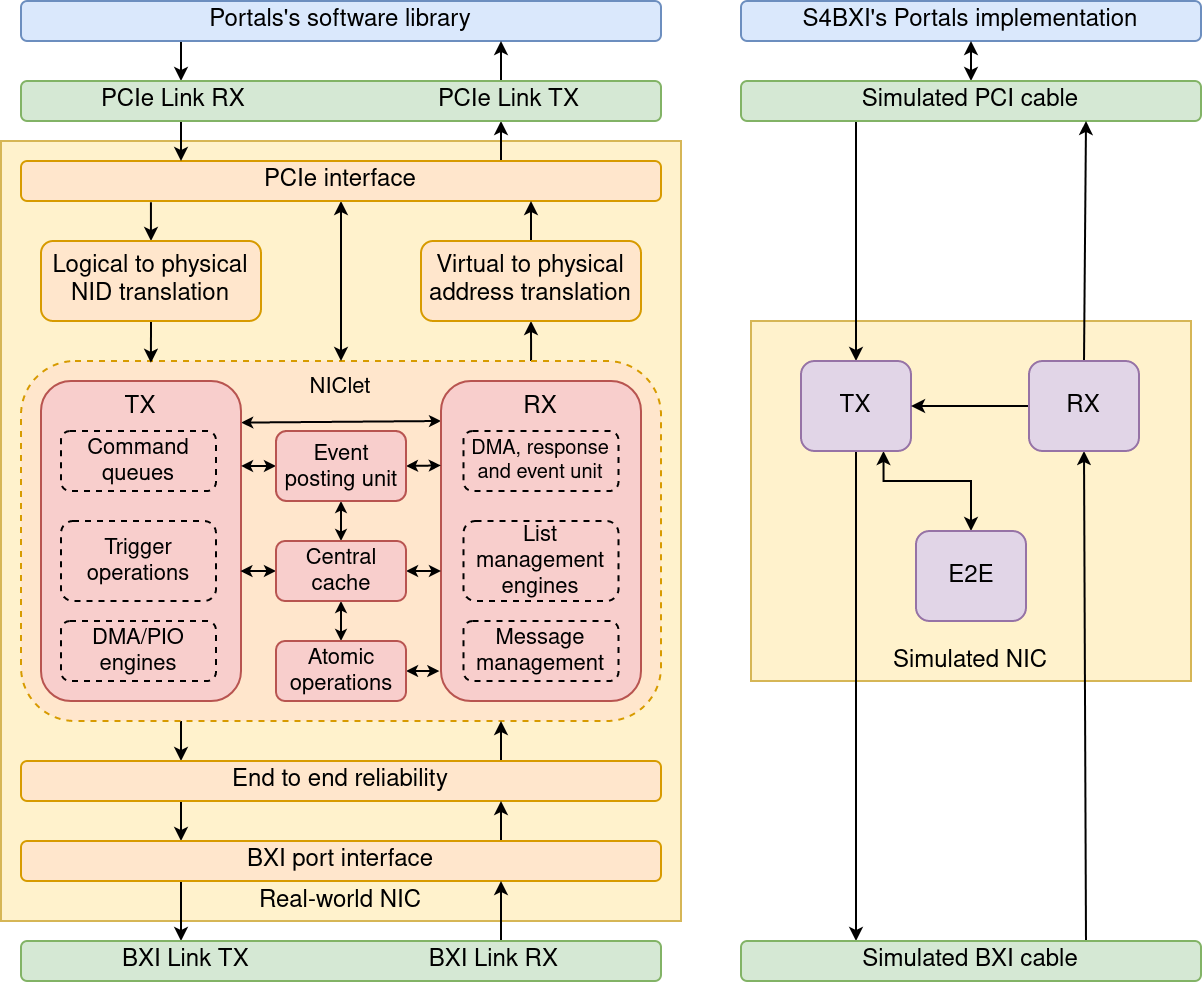
\includegraphics[width=0.9\textwidth]{4_portals/pipeline_comparison.png}
    \caption{Internal pipeline of BXI NICs compared to S4BXI's implementation}
    \label{fig:4_portals:pipeline_comparison}
\end{figure}

Even though there is no particular restriction in Portals itself, in the real
world limitations of the hardware imply that queues have a finite size, and
therefore applications can only buffer a limited number of commands on the NIC
before its command queues run out of space. This phenomenon is modeled in S4BXI,
but in a slightly different way than  in the real-world hardware: as explained
earlier, the real-world NIC features many components that communicate together
through internal queues. This means that the processing of commands goes through
a pipeline, as shown in Figure~\ref{fig:4_portals:pipeline_comparison}. Thanks
to this property, several commands can be in the pipeline at the same time (in
different stages), which gives the software an illusion of parallel processing
(although the vast majority of hardware components are strictly sequential). It
also means that the first component in the pipeline is going to consume commands
faster than we would expect in simulation: in S4BXI the whole processing of a
command is implemented as a single sequential block of code (usually in the TX
Actor's logic), which means that the internal NIC queues that operate on various
packet sizes are not modeled in detail. Because of this, even though we know
that the queues between the CPU and the NIC have 16 entries in them, we need to
increase the queues' size in simulation, in order to account for the depth of
the whole pipeline. From our experimental tests we have determined that a depth
of 89 entries in TX queues in S4BXI give the most accurate result, but it is
important to note that this is only determined empirically, as we do not know in
detail the depth and speed limitations of all intermediate queues inside the
real-world NIC.

\subsubsection{Reusing user buffers}

With Portals, sending data usually triggers two events that are sent by the NIC
to the user application: a SEND event and an ACK event (or REPLY if the targeted
node sends data back, in the case of a FetchAtomic request for example). While
ACK events simply inform the user that the message was successfully delivered
and acknowledged, the SEND event is here to inform the user that the buffer from
which data was sent can be re-used safely. What this last part means is
different depending on the size of the payload: for large messages, the SEND
event will be triggered at the same time as the corresponding ACK, because until
the message is fully acknowledged the NIC could still need to access the payload
in main memory in case of a retransmission by the E2E mechanism. For small
messages (up to 64B), on the other hand, the NIC has enough internal cache
storage to keep the full payload in what is called the``E2E context'' of the
message, which means that in the case of a retransmission the main memory will
not be queried. For this reason, the transfer of small messages can be performed
with a significantly lower latency, and achieve high message rates while having
reliable transfers. This mechanism is fully modeled in the TX Actors of S4BXI,
as we will be able to see in the experimental results of
Section~\ref{sec:4_portals:validation}.

\subsection{Streaming data from memory to memory across BXI}

\subsubsection{Real-world behavior}

When sending data (through any request other than \inline{PtlGet} which
performs a remote ``read'' operation), there are three different ways to move
the payload from the memory to the NIC, which depends on the message size and
options:

For the smallest messages, up to 8B for operations with match bits or 16B
without match bits, the payload can be written ``inline'' in the command
directly, since requests do not use the full memory size available for commands,
according to the command format used to communicate with the NIC.

For larger messages, up to 408 or 416B (again depending on match bits), BXI uses
what is called PIO (Programmed I/O). This method requires the CPU to write the
payload (minus the first 8 or 16B) in a small space of ``scratch'' memory on the
NIC, before sending the command with the remaining data (similarly to inline
mode). This allows data to be accessible right away when the NIC processes the
command, but it costs a small amount of time because it requires the CPU to
perform two PCI writes as well as a memory fence between the two (in order to
make sure data is written before the command).

\begin{figure}[!ht]
    \centering
    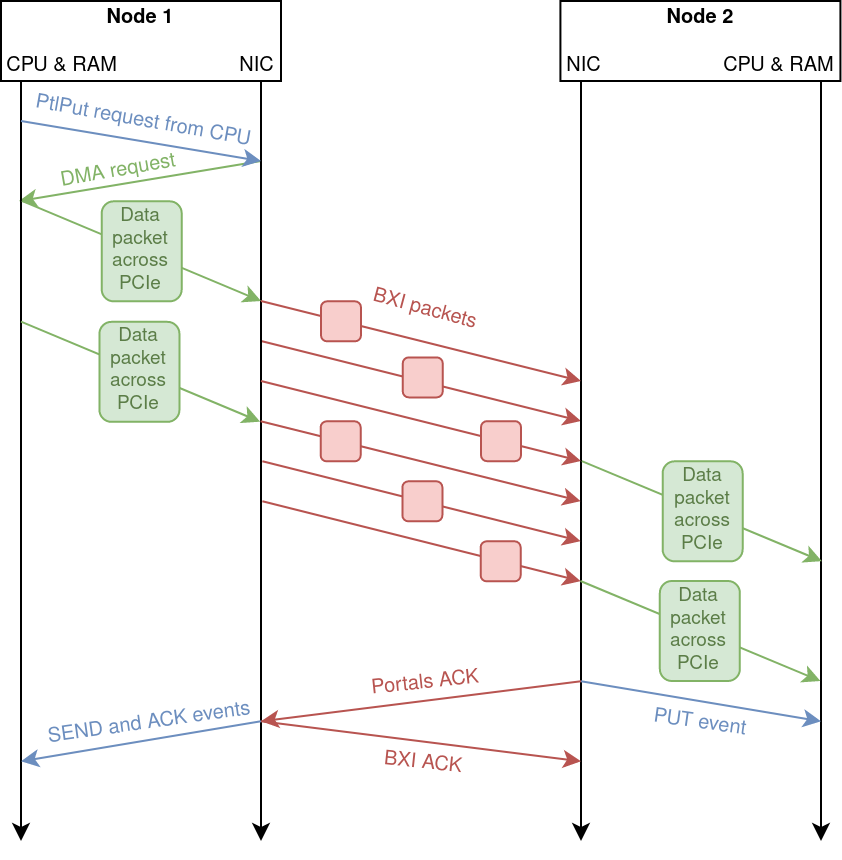
\includegraphics[width=0.9\textwidth]{4_portals/PCI_transfer_real.png}
    \caption{Data transfers when performing a DMA on real hardware}
    \label{fig:4_portals:PCI_transfer_real}
\end{figure}

For the biggest messages, DMA (Direct Memory Access) is used: the CPU simply
sends a command containing the address and length of the memory to be
transferred, and then the NIC reads the memory when it processes the command.
Since the Portals library is mostly operating in userland (and not from a kernel
driver), this means that the addresses sent to the NIC are virtual. This is why
the NIC features a Virtual To Physical (V2P) component which implements the same
page walk through the Memory Management Unit (MMU) as the CPU does, in order to
request the physical memory address and send the data on the network.
Additionally, it is important to note that during a communication using DMA,
three transfers happen in total: a data read across PCI at the sender, the
network transfer, and a data write across PCI at the receiver. Both the sender
and the receiver of the payload synchronize on all three data transfers, which
are dependent on each other: these transfers are all made of packets, and at the
lowest level, flow control guarantees that the data progresses at a rhythm that
is sustainable by both NICs using a flit-level credit system. This means that,
as depicted in Figure~\ref{fig:4_portals:PCI_transfer_real}, PCI packets (which
are typically 512B, even though 256 and 1024B are also supported by BXI) are
broken down into 32B flits, which are then packed into 72B BXI link-level
packets (which contain two flits and 8B of header metadata), and then
re-assembled into PCI packets to be written at the target side.

On the other hand, when sending data back in a response at target side (after a
\inline{PtlGet} for example), the data transfer from memory to the NIC is
always performed in the DMA style, since the targeted machine does not know
which piece of memory might be requested and when.

\subsubsection{Model in S4BXI}

In S4BXI, the inline and PIO transfers are modeled exactly as they happen in the
BXI NIC (with easy to configure thresholds which allow testing different
hypothetical scenarios). The DMA transfers, on the other hand, are by essence
difficult to model because of the nature of our flow model. Indeed, as presented
previously, in the event of a DMA we have three different transfers that are all
dependent on each other, and this dependency can only be described accurately by
modeling each packet. This section will present several ways to model these
transfers, starting with the most naive and ending with the model that is
currently implemented in our simulator.

\begin{figure}[!ht]
    \centering
    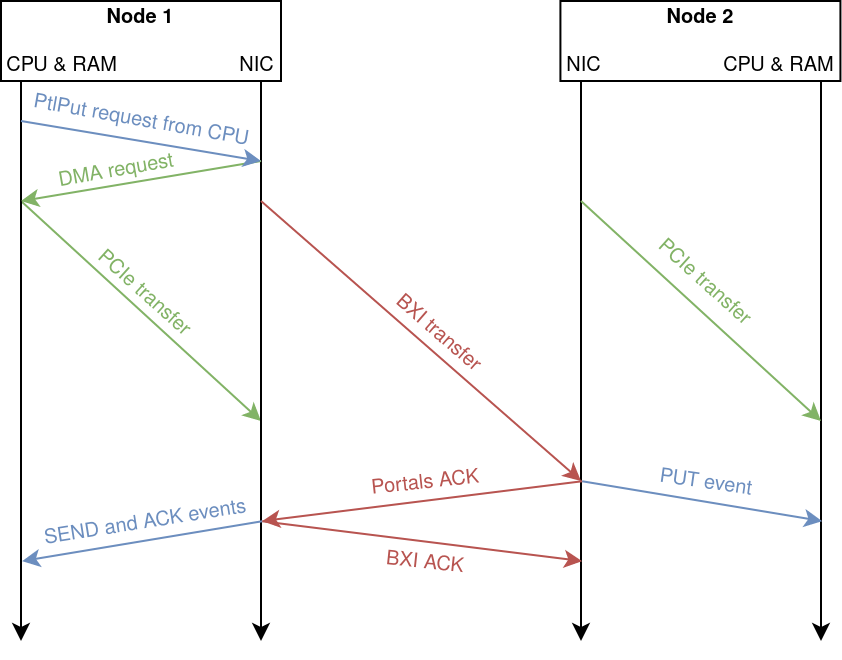
\includegraphics[width=0.9\textwidth]{4_portals/PCI_transfer_naive.png}
    \caption{Naive flow model of data transfers when performing a DMA}
    \label{fig:4_portals:PCI_transfer_naive}
\end{figure}

A naive way to model this would be to start all three transfers at the same time
in simulation (since they are very well pipelined in real life), as depicted in
Figure~\ref{fig:4_portals:PCI_transfer_naive}. While this is a good
approximation for moderate workloads, it loses significant accuracy if there is
congestion on any of the transfers. In particular, the PCI write at the receiver
will progress even if the BXI transfer gets slowed down by congestion. This
results in an overly optimistic simulator in the case of communication-intensive
workloads.

\begin{figure}[!ht]
    \centering
    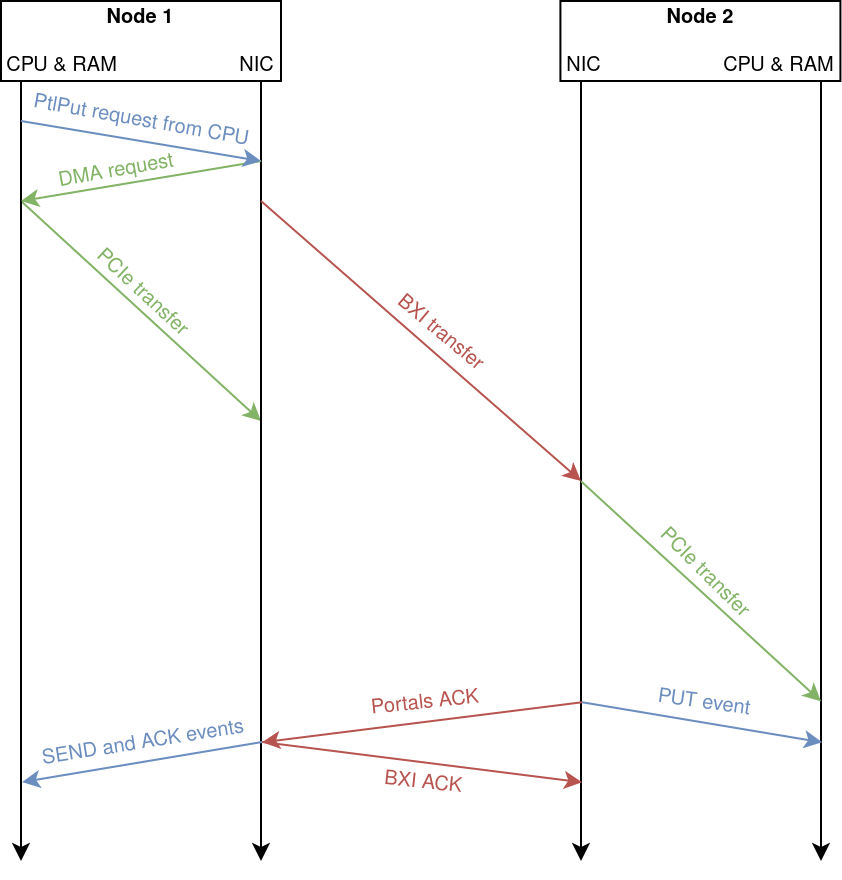
\includegraphics[width=0.9\textwidth]{4_portals/PCI_transfer_late_events.png}
    \caption{Flow model of data transfers when performing a DMA, accounting for network congestion}
    \label{fig:4_portals:PCI_transfer_late_events}
\end{figure}

A different option to model this scenario is to perform the PCI write at target
only when the network transfer across BXI is complete, as depicted in
Figure~\ref{fig:4_portals:PCI_transfer_late_events}. While this model accounts
for congestion across the BXI network, it is very pessimistic in most cases,
effectively reducing the maximum achievable bandwidth to half the bandwidth of
the BXI cables, since the BXI transfer and the PCI write are performed sequentially.

\begin{figure}[!ht]
    \centering
    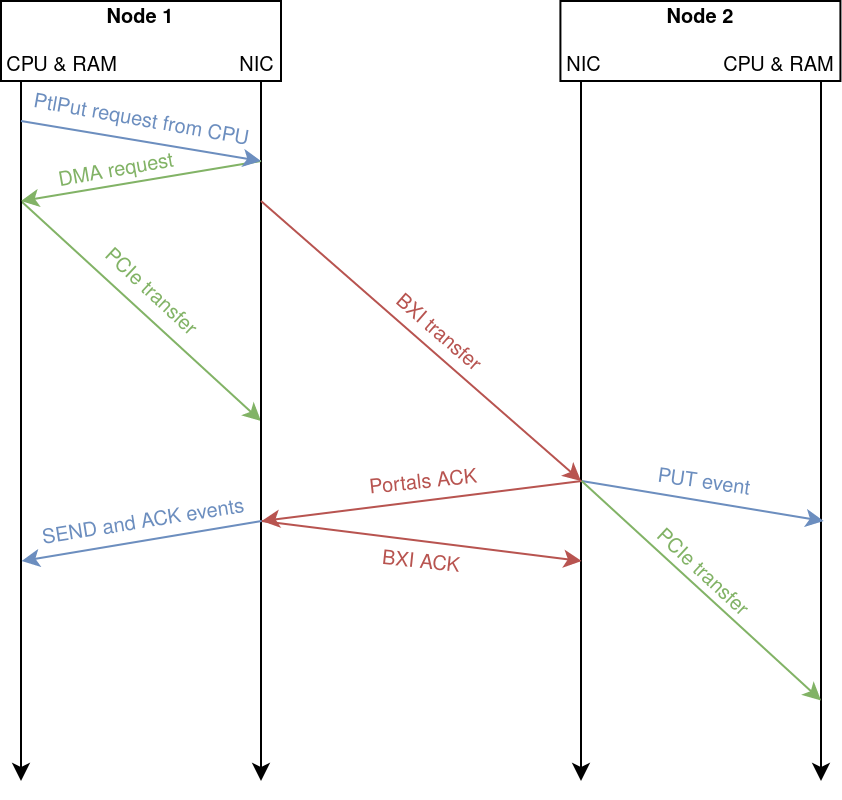
\includegraphics[width=0.9\textwidth]{4_portals/PCI_transfer_early_events.png}
    \caption{Flow model of data transfers when performing a DMA, with asynchronous PCI writes}
    \label{fig:4_portals:PCI_transfer_early_events}
\end{figure}

Finally, a solution to delay the PCI write while generating Portals events and
acknowledgements faster is to perform the PCI write asynchronously in the
background, as depicted in Figure~\ref{fig:4_portals:PCI_transfer_early_events}.
While this is still very far from a perfect model, it will generate a more
realistic congestion on the PCI bus at receiver side, which will impact the
generation of PUT events for example.

It is important to note that in any case, all these models are only realistic
for large data transfers, in which the payload is composed of many PCI packets.
Indeed, we can see on Figure~\ref{fig:4_portals:PCI_transfer_real} that even
though the three types of transfers are very well pipelined, the first PCI
packet at sender side needs to be fully received before initiating the transfer
across BXI, and at receiver side, the BXI transfer needs to be fully completed
before starting to write the last PCI packet. This means that for messages which
can fit in a few PCI packets, the pipeline will not allow the transfers to
overlap perfectly. The most pathologic case would be for messages that fit in a
single PCI packet (so smaller than 512B), for which there is no pipelining at
all, and the three transfers are essentially sequential. In S4BXI we account for
this effect by adding a small sleep inside TX Actors before starting the
transfer across BXI, and another similar sleep in RX Actors before generating
Portals events and any acknowledgement. Therefore, the final sequence of
transfers that is implemented in S4BXI corresponds to
Figure~\ref{fig:4_portals:PCI_transfer_simu_final}.

\begin{figure}[!ht]
    \centering
    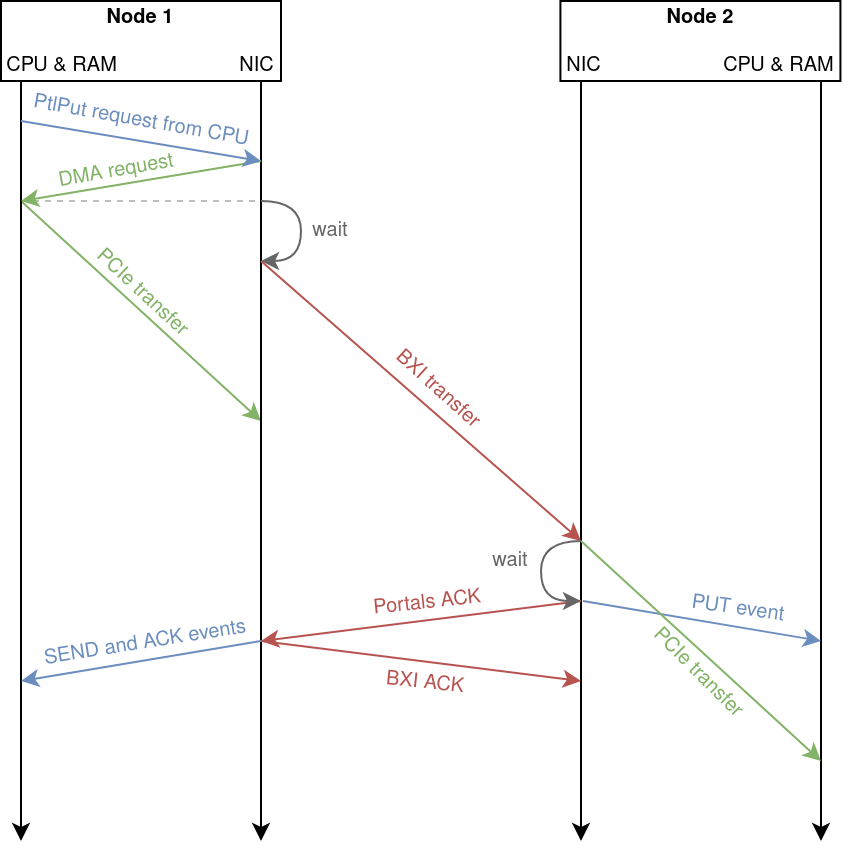
\includegraphics[width=0.9\textwidth]{4_portals/PCI_transfer_simu_final.png}
    \caption{Flow model of data transfers when performing a DMA, as implemented in S4BXI}
    \label{fig:4_portals:PCI_transfer_simu_final}
\end{figure}

Finally, it is also important to mention that all transfers that are represented
in each figure only model the time that operations take in our simulator: since
our simulation is single-threaded, the data that is exchanged between two NICs
is available at the target instantly by exchanging a C pointer. Therefore, it is
not erroneous to issue a PUT event before the end of the PCI write at target
side, as the RX side of our simulated NIC can access the payload at any point.

\subsection{Performance options}

In a first attempt to customize the performance/accuracy tradeoff of the
simulator, we have implemented several options that can simplify the processing
inside our simulated NICs:

\subsubsection{Quick ACKs}

Very often, messages containing data (\inline{PtlPut} requests for example) are
much heavier than lightweight acknowledgements, and will account for the
majority of the time spent performing network operations on a real-world
cluster. Therefore, S4BXI allows generating ACK events instantaneously instead
of creating a proper ACK message and sending it on the network. This means that
in this case, ACK events at sender side are going to be generated from an RX
Actor at the \textbf{receiver} side, which is obviously possible in simulation
only (since it would require a network communication in the real world). If E2E
processing is active, enabling this option saves not only one but two small ACK
messages: the Portals ACK used to generate the ACK event, and the BXI ACK used
by E2E internally, as depicted in Figure~\ref{fig:4_portals:quick_acks}

\begin{figure}[!ht]
    \centering
    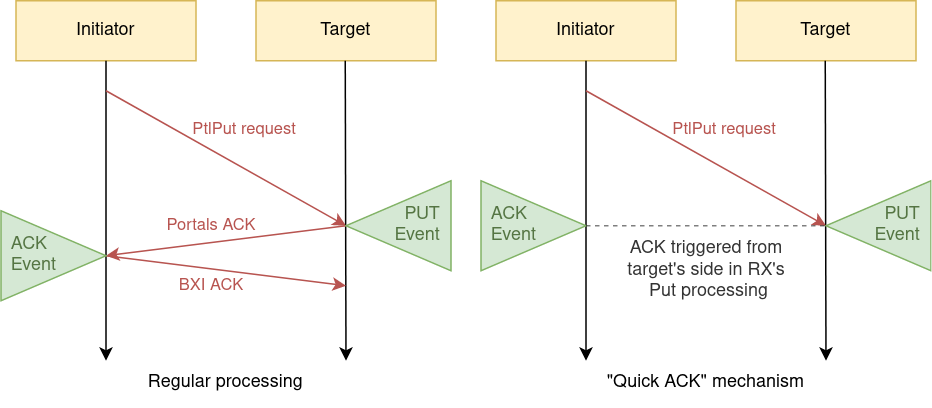
\includegraphics[width=1\textwidth]{4_portals/quick_acks.png}
    \caption{Quick ACK mechanism in S4BXI}
    \label{fig:4_portals:quick_acks}
\end{figure}

\subsubsection{Simplified PCI model}

In the same spirit as Quick ACKs, S4BXI supports ignoring small PCI transfers:
if messages of a consequent size are exchanged on the network, the time spent
exchanging lightweight commands across the PCI bus in real world is usually
negligible compared to data transfers (writes at target side or reads at
initiator side). Therefore, S4BXI provides an option to ignore them and save a
few operations in SimGrid's kernel, which is controlled either globally using
the \inline{S4BXI_MODEL_PCI_COMMANDS} environment variable, or on an Actor per
Actor basis using the \inline{model_pci_commands} property in the simulation's
deployment. A more aggressive optimization consists in disabling every PCI
transfer (including data transfers) completely. While this can increase
performance a bit more, it is much less realistic. Similarly, this option can be
enabled globally using the \inline{S4BXI_MODEL_PCI} environment variable, or
locally using the \inline{model_pci} property on individual Actors.

\section{Tracing and Visualization System}

While SimGrid provides a low-level tracing system, which allows logging all
activity on compute resources, links, etc., we felt the need to create our own
too. Since it operates at Portals level, our system can add more metadata to
operations: this provides a precise log of the different request and response
types, whereas SimGrid's low-level system only provides the usage of each Link,
without any information on the type of Portals operation.

Tracing in S4BXI is disabled by default. To enable it, one simply sets the
environment variable \inline{S4BXI_LOG_FOLDER} to a valid path. S4BXI will
then write logs of all operation in CSV format (for easier parsing), splitting
the log file every 10,000 lines. Additionally, the variable
\inline{S4BXI_LOG_COMPUTATION} controls whether CPU operations should be
logged, or only network ones (since CPU operations can be very numerous, and not
necessarily the main point of interest).

\begin{figure}[!ht]
    \lstinputlisting[basicstyle=\ttfamily\footnotesize,frame=bt,language=C++]{4_portals/bxi_log_type.cpp}
    \caption{Event types in S4BXI's tracing system}
    \label{fig:4_portals:bxi_log_type}
\end{figure}

\begin{figure}[!ht]
    \centering
    \includegraphicsOverflow{4_portals/S4BXI_trace.png}{1.15}
    \caption{Example trace from S4BXI, two simple Put requests between NID 1 and 2}
    \label{fig:4_portals:S4BXI_trace}
\end{figure}

The different types of events logged by S4BXI is described in the enum
\inline{bxi_log_type}, which is shown in
Figure~\ref{fig:4_portals:bxi_log_type}. The output CSV files can be easily
parsed, but to simplify their visualization we developed a small online
tool\footnote{Hosted at \url{https://s4bxi.julien-emmanuel.com/log-viewer/}} to
display operations in a sequence graph. While it does not scale very well when
the number of nodes involved is important, it is a useful tool to debug at a
small scale, and its code\footnote{Open source at
\url{https://framagit.org/s4bxi/s4bxi-log-viewer}} gives a simple example of how
to use the trace files. A screenshot of an example output of our tool is
displayed on Figure~\ref{fig:4_portals:S4BXI_trace}.

\section{Additional implementation considerations}

\subsection{Practical usage of S4BXI, and simulated process isolation}
\label{subsec:4_portals:process_isolation}

\begin{figure}[!ht]
    \centering
    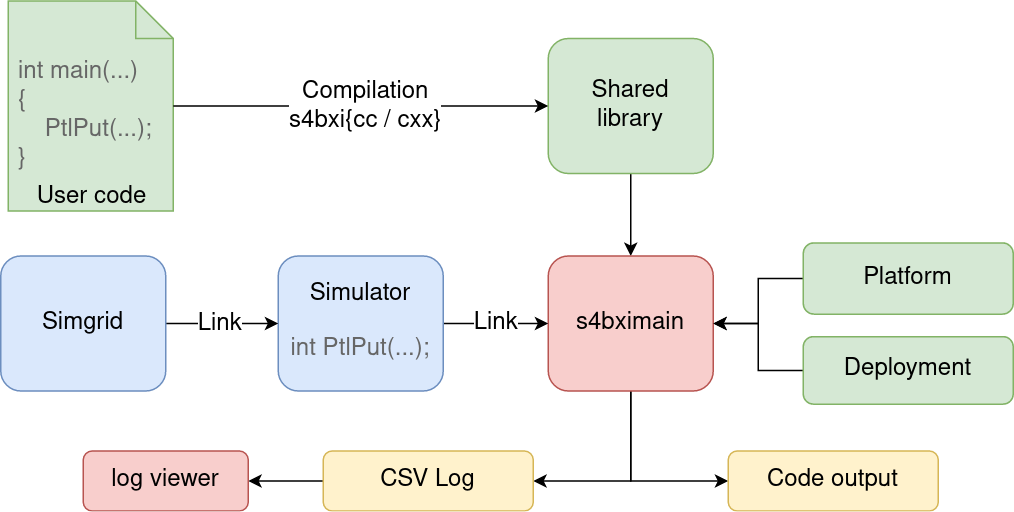
\includegraphics[width=0.9\textwidth]{4_portals/s4bxi_usage.png}
    \caption{S4BXI components and usage}
    \label{fig:4_portals:s4bxi_usage}
\end{figure}

To facilitate the configuration of the compiler for S4BXI users we provide
scripts that act as wrappers around compilers (namely \inline{s4bxicc} and
\inline{s4bxicxx}) that have a very similar goal than the corresponding
\inline{smpicc} and \inline{smpicxx}: make the compiled program a shared
library, and include header files to redefine the symbols that we want to
capture (using C macros). An overview of the methodology is shown on
Figure~\ref{fig:4_portals:s4bxi_usage}: First the application's code is
compiled, either with our compiler wrappers directly or simply by adding the
\inline{-shared} flag manually. Then S4BXI is started (through the binary
\inline{s4bximain}) with three essential arguments: the simulated platform's
description, the associated deployment configuration, and finally the shared
library which contains the application. Each Actor which runs the user
application will then copy the application's library on disk with a different
name for each simulated process, and use the \inline{dlopen} and \inline{dlsym}
function to extract the \inline{main} symbol from the library and run it. The
reason for copying the simulated application (instead of opening the same
library from every simulated process) is that it allows us to trick the dynamic
linker into thinking that all these copies are different libraries, which allows
us to leverage the linker's ability to isolate the global symbols (in particular
global variables) of different libraries running in the same address space. This
provides isolation between the different simulated processes even though they
all run in a single thread in practice, without having to implement this feature
ourselves.

\subsection{Platform implementation in S4BXI}

At the beginning of this PhD, the most popular way of describing SimGrid
platforms was using a static XML document\footnote{The corresponding DTD is
available at \url{https://simgrid.org/simgrid.dtd}}. Unfortunately, this wasn't
a very flexible approach: there are XML tags that try to simplify the platform,
such as \inline{<cluster>} which creates the complete list of Hosts and Links
for common topologies, but unfortunately when using these the ``leaf'' nodes of
the cluster could only be simple Hosts (instead of the more complete model with
PCI cables, etc. that we described above). For this reason we made some scripts
to convert the output of real-world cluster management software (BXI-AFM in our
case) into a SimGrid XML platform that comply with S4BXI's requirements. While
this is a functional solution, it had the downside of generating potentially
very heavy and verbose platforms, which could take a significant amount of time
and memory to parse in SimGrid. Thankfully, since then the SimGrid team
developed a C++ API (integrated in S4U) to describe platforms, which is
significantly more performant and flexible. We added support for it in our
simulator by checking the filetype of the platform at startup (either an XML
file or a shared library compiled from a C++ platform), and in the case of a C++
platform our simulator looks for a specific symbol (\inline{load_platform}) to
call, which is responsible for generating the platform. While we kept the
support for XML platforms, all our experiments will use the C++ API, which
should become the standard way of using SimGrid in the future.

\subsection{Portals's implementation in C/C++}

\begin{figure}[!ht]
    \centering
    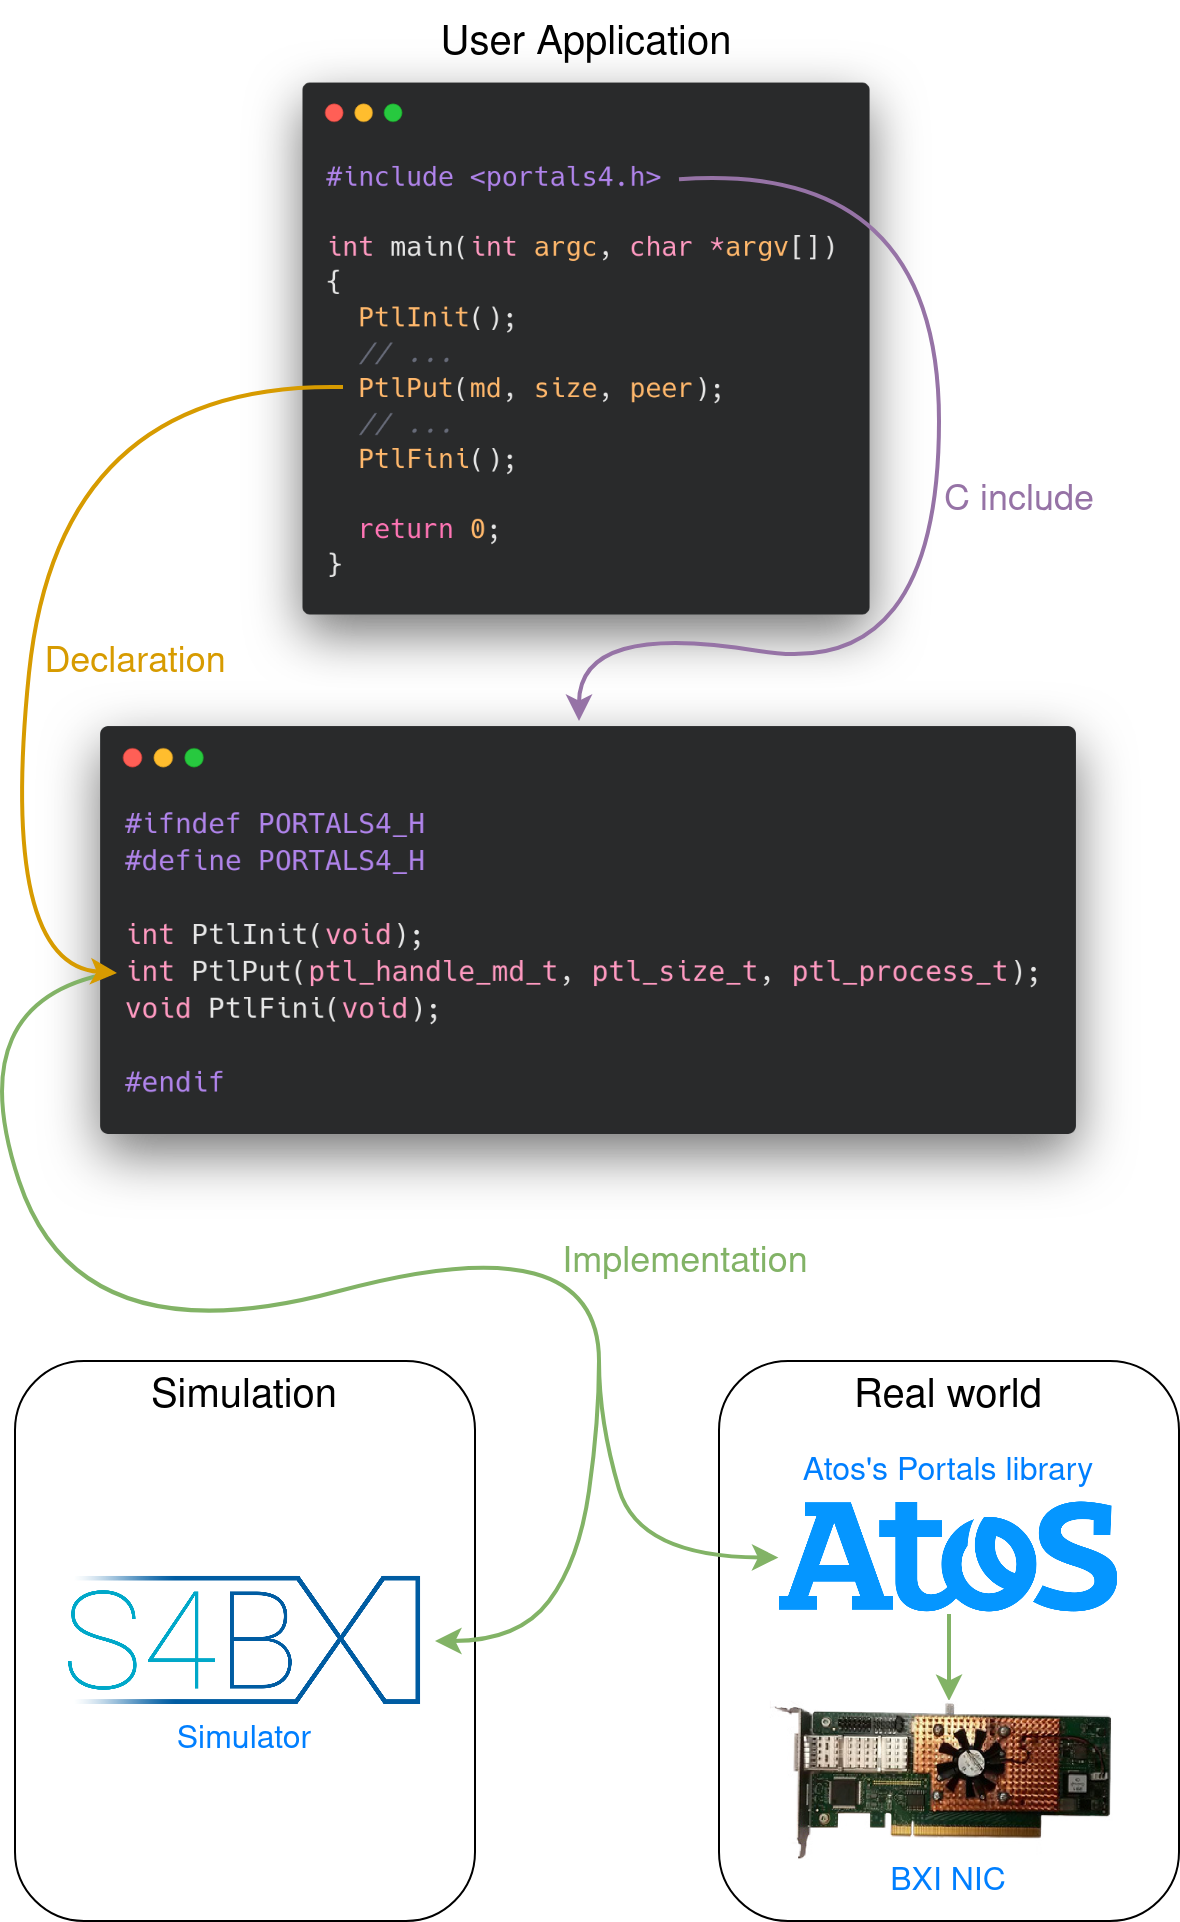
\includegraphics[width=0.7\textwidth]{4_portals/portals_h.png}
    \caption{Declaration and implementation of Portals's primitives}
    \label{fig:4_portals:portals_h}
\end{figure}

On a real cluster, the user code (or a library such as MPI) includes the
\inline{portals4.h} header file, which provides the declarations for Portals's
structures and primitives. In simulation, we simply reuse the
\inline{portals4.h} header provided by the real world implementation made by
Atos (as well as a few BXI-specific helpers for an optimal compatibility,
\inline{portals4_bxiext.h} and \inline{portals4_services.h}). These files allow
us to have identical declarations, so that user code can use our simulated
Portals or Atos's one transparently. The difference comes from the
implementation: while the Portals primitives are implemented by Atos's library
on a real cluster, in simulation S4BXI provides an implementation on top of
SimGrid. This methodology is represented on
Figure~\ref{fig:4_portals:portals_h}, in which we can see how the difference
between real-world and simulation comes only from the implementation of
primitives.

Internally all our Actors are implemented by C++ classes, as SimGrid is very
flexible in this regard: Actors' behavior can be implemented either using a
simple function, a class, or anything that is callable (our complete class
hierarchy is represented in Appendix~\ref{app:s4bxi_class_hierarchy}. Therefore,
the implementation behind the public interface is simply a small layer that
retrieves the current S4BXI Actor instance (\inline{BxiMainActor} in our class
hierarchy) and calls a member function corresponding to the desired Portals
primitive. This lookup of the current S4BXI Actor instance is optimized using a
small plugin we wrote for SimGrid, which allows us to store this pointer in
SimGrid's representation of Actors.

\subsection{Capturing function calls}

While the Portals primitives naturally link with S4BXI's implementation in
simulation, there are other function calls that need to be
intercepted: all utilities that rely on time, such as
\inline{gettimeofday}, \inline{sleep}, etc. must be
re-implemented in simulation in order to use simulated time instead of
wall-clock time. A traditional way to perform this interception is to preload a
library using the \inline{LD_PRELOAD} environment variable on Linux. While
this is efficient, we chose a simpler approach (similar to SMPI) where the
function calls that we re-implent are redirected to the simulator's
implementation using \inline{#define} C macros. This method is more intrusive
since it requires re-compiling the simulated application, but in our workflow it
does not add any constraint since we already need to compile the application, in
order to make a shared library (as explained in
Subsection~\ref{subsec:4_portals:UserAppActors}).

In S4BXI we implemented most functions that can be used to sleep with various
precision (\inline{sleep}, \inline{nanosleep}, etc.), functions to query the
current time (\inline{gettimeofday}, \inline{clock_gettime}, etc.) as well as a
few other utilities such as \inline{hostname}, \inline{getpid}, etc. so that
each simulated node returns a value from the simulated world instead of data
from the machine running the simulation. We also support a subset of signal
handlers that we encountered in low-level benchmarks: \inline{sigaction} stores
the handler for a given signal in a simulated-Actor specific structure, and this
handler is then executed after a call to \inline{setitimer} or \inline{alarm}
and the corresponding waiting time is elapsed in the simulated world. In order
to wait for the desired amount of time, and call the appropriate handler when
the timeout expires, we spawn a short-lived Actor so that the main application
can continue to progress at the same time, as it would in real-life (since the
timer runs in the background).

\subsection{Completeness}

S4BXI was made with the end goal of simulating high-level APIs, in particular
MPI, and therefore we only implemented the features that we needed for this
purpose. This means that our Portals implementation is not complete, although
the majority of Portals primitives are supported (and tested in our Continuous
Integration). The main missing features are I/O Vectors (IOVEC), which are the
ability to send several pieces of non-contiguous data at once, as well as
triggered operations, which are the ability to send a message automatically when
a specific event happens in Portals. We only left these features aside because
of time constraints, and we believe that the current architecture of our
simulator would make their implementation straightforward. Adding these features
would only be a matter of investing some engineering time, if there was a need
for it, since they would be very similar to the existing logic currently
implemented in the simulator.

\section{Experimental validation}
\label{sec:4_portals:validation}

In order to get a first validation of our Portals model (before moving on to
higher-level APIs) we executed two types of benchmark on a BXI cluster and in
S4BXI: first we started with custom-made tests, which are very simplistic, and
then we ran PtlPerf, which is a pre-existing tool made at Atos to perform
point-to-point performance measurements, as presented in
Section~\ref{sec:2_context_hpc:benchmarks}.

\subsection{Custom made benchmarks}

While we check that all request types are functionnally correct in our
Continuous Integration, we studied in more detail \inline{PtlPut} and
\inline{PtlGet} operations in order to validate their performance in simulated
time against real-world executions on BXI hardware. Indeed, it is easy to write
a test suite to ensure that all operations transfer data correctly, but
evaluating the accuracy of the simulator is significantly harder to automate. We
chose to study these primitives because they are the most commonly used, in
particular they are the only request types that are used in the MPI
implementation that we will study in the next chapter.

\subsubsection{Benchmarks' behavior}

Each benchmark that we made operates on the same principle: 10,000 requests (Put
or Get) are sent from a machine A to a machine B, while both machines measure
the total time. This workload is repeated for 64 different message sizes,
which are chosen according to the following method: the first few message sizes
are hardcoded and correspond to the sizes where we expect significant changes in
the duration of the benchmark (because of the optimizations that we know exist
in the real-world hardware and the S4BXI model), for example at 64B (and
therefore 65B too in order to see the change clearly). Then, the next sizes are
generated at random, using a distribution uniform on a log scale (in base two).
We did not go for powers of two directly, to avoid testing only very particular
values. We also did not go for a simple uniform distribution because we are more
interested in small values, for which there are more variations in the
performance of BXI.

We designed five types of benchmarks: three for the \inline{PtlPut} operation
and two for \inline{PtlGet}. To make this section easier to read, we will name
each of these variants, and illustrate them with sequence diagrams (which offer
a simplified representation of the transfers involved, in particular they are a
lot less detailed than figures~\ref{fig:4_portals:PCI_transfer_naive}
to~\ref{fig:4_portals:PCI_transfer_simu_final}):

\begin{description}
    \item[Put-WaitAck] performs Put operations. The benchmark waits for an ACK
    event before moving on to the next operation, which means that there is only
    one message inflight at all times. This corresponds to the sequence diagram
    on Figure~\ref{fig:4_portals:ptlput_waitack_seq}.
    \item[Get-WaitReply] performs Get operations. The benchmark waits for a
    REPLY event before moving on to the next operation, so once again there is
    only one message inflight at all times. This corresponds to the sequence
    diagram on Figure~\ref{fig:4_portals:ptlget_waitreply_seq}.
    \item[Put-NoWait] performs Put operations as fast as possible, without
    waiting for any event. While this workload is not a very realistic use of
    BXI NICs, it allows us to benchmark the ability of the NIC to absorb and
    process many commands, and to see how the network performs when many
    messages are inflight at the same time. This corresponds to the sequence
    diagram on Figure~\ref{fig:4_portals:ptlput_nowait_seq}.
    \item[Get-NoWait] performs Get operations as fast as possible, without
    waiting for any event. Once again this benchmark allows us to stress the
    NICs involved, in particular the target NIC which will receive many requests
    at a high rate. This corresponds to the sequence diagram on
    Figure~\ref{fig:4_portals:ptlget_nowait_seq}.
    \item[Put-WaitSend] performs Put operations. The benchmark waits for a SEND
    event before moving on to the next operation. This is closer to a realistic
    use case of Portals, as this event indicates that the source buffer can be
    safely reused. In practice, it allows small messages to be processed in a
    pipelined way, while for large messages it is equivalent to waiting for the
    ACK event. This corresponds to the sequence diagram on
    Figure~\ref{fig:4_portals:ptlput_waitsend_seq}.
\end{description}

\begin{figure}[!h]
    \centering
    \begin{subfigure}{.5\textwidth}
        \centering
        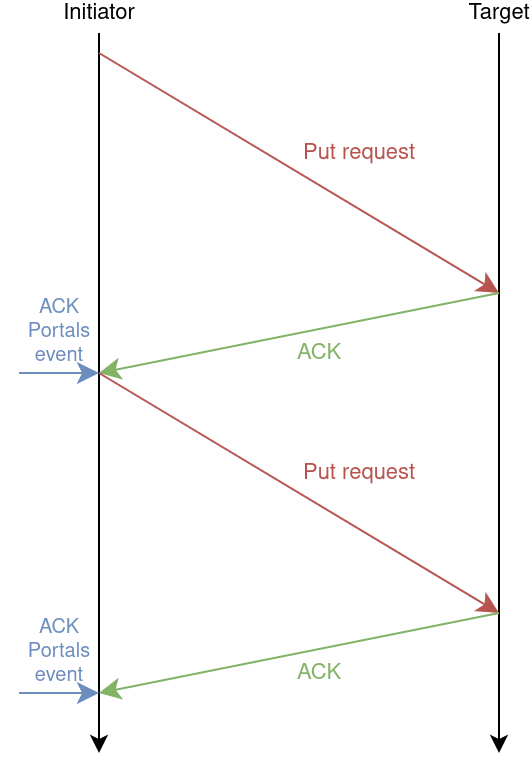
\includegraphics[width=1\linewidth]{4_portals/bench_put_waitack.png}
        \caption{\inline{PtlPut} variant (\textbf{Put-WaitAck})}
        \label{fig:4_portals:ptlput_waitack_seq}
    \end{subfigure}% this comment is important otherwise the images are vertical
    \begin{subfigure}{.5\textwidth}
        \centering
        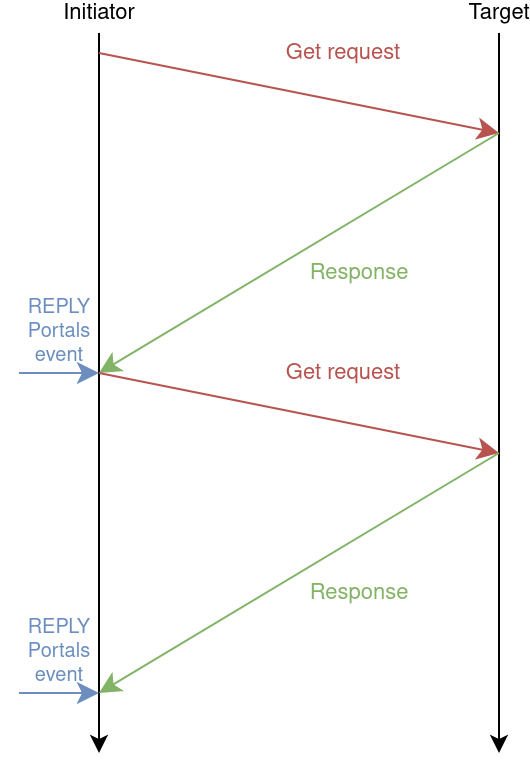
\includegraphics[width=1\linewidth]{4_portals/bench_get_waitreply.png}
        \caption{\inline{PtlGet} variant (\textbf{Get-WaitReply})}
        \label{fig:4_portals:ptlget_waitreply_seq}
    \end{subfigure}
    \caption{Portals experiment, one request at a time}
    \label{fig:4_portals:ptl_wait_seq}
\end{figure}

\begin{figure}[!h]
    \centering
    \begin{subfigure}{.5\textwidth}
        \centering
        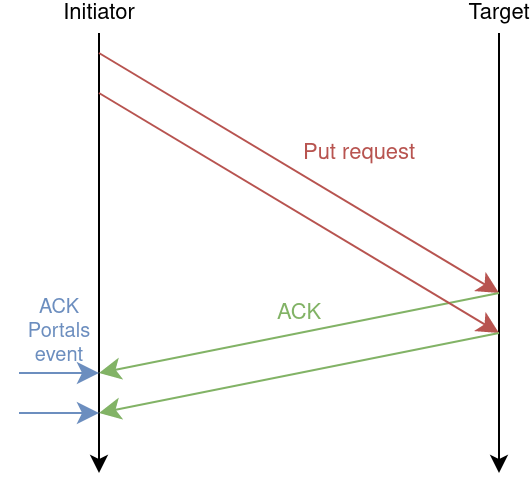
\includegraphics[width=1\linewidth]{4_portals/bench_put_nowait.png}
        \caption{\inline{PtlPut} variant (\textbf{Put-NoWait})}
        \label{fig:4_portals:ptlput_nowait_seq}
    \end{subfigure}% LaTeX is garbage
    \begin{subfigure}{.5\textwidth}
        \centering
        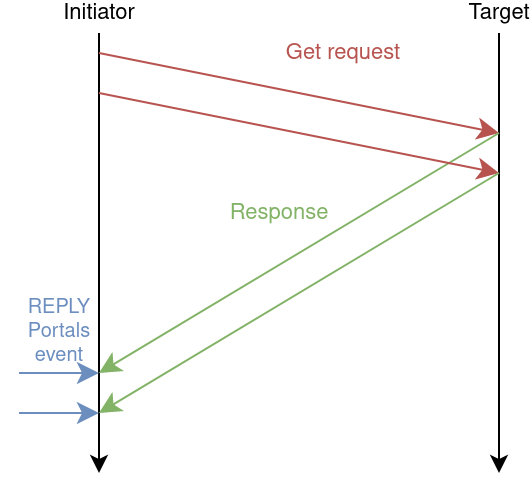
\includegraphics[width=1\linewidth]{4_portals/bench_get_nowait.png}
        \caption{\inline{PtlGet} variant (\textbf{Get-NoWait})}
        \label{fig:4_portals:ptlget_nowait_seq}
    \end{subfigure}
    \caption{Portals experiment, sending requests as fast as possible}
    \label{fig:4_portals:ptl_nowait_seq}
\end{figure}

\begin{figure}[!h]
    \centering
    \begin{subfigure}{.5\textwidth}
        \centering
        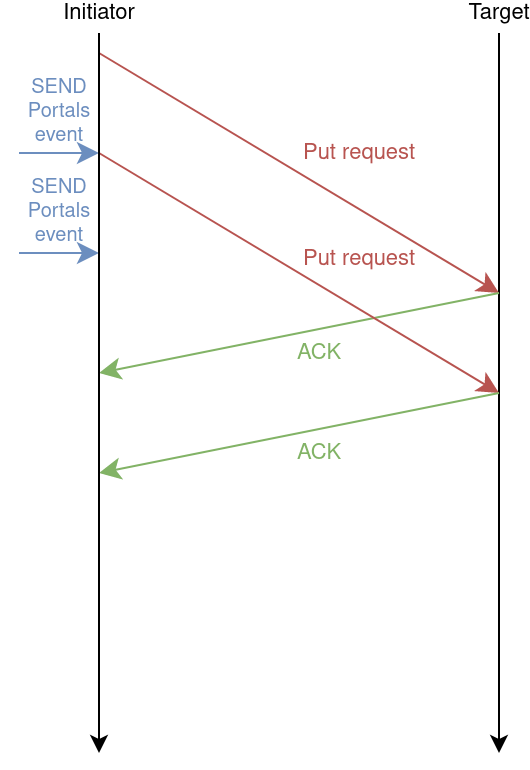
\includegraphics[width=1\linewidth]{4_portals/bench_put_waitsend_small.png}
        \caption{Messages smaller than 64B}
        \label{fig:4_portals:ptlput_waitsend_small_seq}
    \end{subfigure}% LaTeX is garbage
    \begin{subfigure}{.5\textwidth}
        \centering
        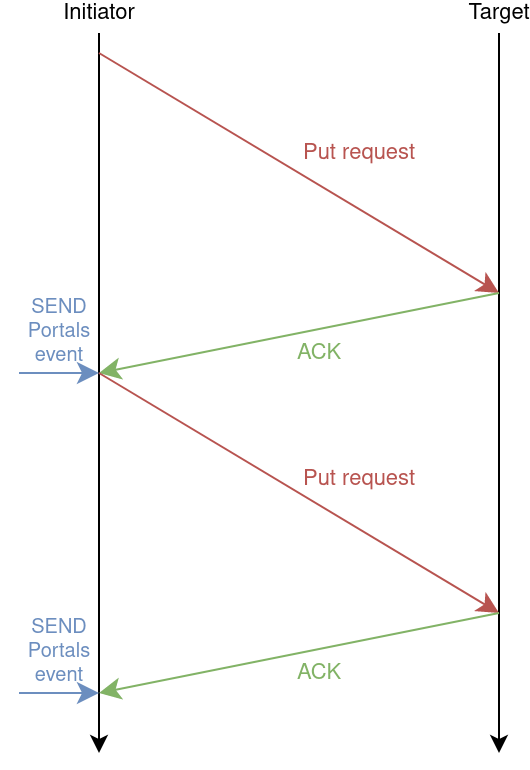
\includegraphics[width=1\linewidth]{4_portals/bench_put_waitsend_big.png}
        \caption{Messages bigger than 64B}
        \label{fig:4_portals:ptlput_waitsend_big_seq}
    \end{subfigure}
    \caption{\inline{PtlPut} experiment, waiting for SEND event between requests (\textbf{Put-WaitSend})}
    \label{fig:4_portals:ptlput_waitsend_seq}
\end{figure}

As illustrated on figure~\ref{fig:4_portals:ptl_wait_seq}, the
\textbf{Put-WaitAck} and \textbf{Get-WaitReply} benchmarks are very simplistic,
as they evaluate the total latency of an operation, which includes an initial
message and a response (either a full reply or a small ACK). On the other hand,
Figure~\ref{fig:4_portals:ptl_nowait_seq} shows that the \textbf{Put-NoWait} and
\textbf{Get-NoWait} benchmarks stress both NICs involved much more, by
requesting as many operations inflight as possible, which evaluates the capacity
of the hardware to process commands and incoming messages in a pipelined way.
Finally, \textbf{Put-WaitSend} corresponds to a more realistic usage of the
hardware.

\subsubsection{Experimental setup}

When simulating these benchmarks, we observed that our simplistic CPU model
caused the simulations to be overly pessimistic (to the point where putting a
zero nanosecond latency on all Links of our simulated platform still gave
pessimistic results). We concluded that since our benchmarks are focused on the
network, the CPU sections between two network primitives are very short, and
that the latency of starting and stopping our CPU timer impacted its
measurements in a very significant way, resulting in pessimistic CPU times. To
fix this problem, we can configure the CPU model to ignore computations that are
shorter than a supplied threshold, therefore for these experiments we ignored
all computations smaller than one microsecond, which effectively ignores all
computation phases in this specific case (since the CPU time is only spent
executing a \inline{for} loop around the network primitives essentially).

From a technical point of view, in the real-world cluster the nodes we use are
equipped with BXI v2 hardware and AMD EPYC™ 7763 64-Core processors. For the
simulations we use a traditional desktop computer, which has an Intel® Core™
i9-10850K CPU and 32 GB of RAM. For each message size the experiment is executed
five times on the real-world cluster in order to ensure that the results are
consistent, and only once in simulation since it is fully deterministic and
reproducible.

\subsubsection{Results}

The results of our benchmarks are displayed on the following figures:
\begin{itemize}
    \item Figure~\ref{fig:4_portals:ptlput_waitack} shows the result of the
    \textbf{Put-WaitAck} benchmark
    \item Figure~\ref{fig:4_portals:ptlput_nowait} shows the result of the
    \textbf{Put-NoWait} benchmark
    \item Figure~\ref{fig:4_portals:ptlput_waitsend} shows the result of the
    \textbf{Put-WaitSend} benchmark
    \item Figure~\ref{fig:4_portals:ptlget_waitreply} shows the result of the
    \textbf{Get-WaitReply} benchmark
    \item Figure~\ref{fig:4_portals:ptlget_nowait} shows the result of the
    \textbf{Get-NoWait} benchmark
\end{itemize}

\begin{figure}[!h]
    \centering
    \includegraphicsOverflow{4_portals/custom/put_waitack.png}{1.2}
    \caption{\textbf{Put-WaitAck} benchmark}
    \label{fig:4_portals:ptlput_waitack}
\end{figure}

\begin{figure}[!b]
    \centering
    \includegraphicsOverflow{4_portals/custom/put_nowait.png}{1.2}
    \caption{\textbf{Put-NoWait} benchmark}
    \label{fig:4_portals:ptlput_nowait}
\end{figure}

\begin{figure}[!b]
    \centering
    \includegraphicsOverflow{4_portals/custom/put_waitsend.png}{1.2}
    \caption{\textbf{Put-WaitSend} benchmark}
    \label{fig:4_portals:ptlput_waitsend}
\end{figure}

\begin{figure}[!b]
    \centering
    \includegraphicsOverflow{4_portals/custom/get_waitreply.png}{1.2}
    \caption{\textbf{Get-WaitReply} benchmark}
    \label{fig:4_portals:ptlget_waitreply}
\end{figure}

\begin{figure}[!h]
    \centering
    \includegraphicsOverflow{4_portals/custom/get_nowait.png}{1.2}
    \caption{\textbf{Get-NoWait} benchmark}
    \label{fig:4_portals:ptlget_nowait}
\end{figure}

Each graph shows the overall duration of the benchmark, the bandwidth, and the
message rate, estimated by our simulator in red (with circular points) and as
reported by real-world runs on the BXI cluster in blue (with triangular points).
It is important to note that all graphs use a log scale on both axes (a base two
log on the x-axis and a base ten log on the y-axis), in order to make results
more readable. In particular, on all variants of our experiments, the left side
shows experiments on small messages, therefore the duration of operations
correspond to the latency of the hardware, whereas on the right side the
duration of operations is dominated by the bandwidth of network cables. This
explains why for large messages, all benchmarks exhibit the same behavior (which
is perfectly captured by our simulator, as it is the easiest workload to model).

While most results given by our simulator are very good, there are a few notable
things to see in these graphs: first, the benchmarks that perform one request at
a time give excellent results in simulation. This is because these benchmarks
mainly evaluate the latency of the network, which we can tune easily, without
caring about the ability of the NIC to process requests in parallel (or at least
in a pipelined way). On the other hand, benchmarks which send requests as fast
as possible give results which are further from reality: it is harder to model
these cases because the performance of the benchmark depends on the ability of
the NIC to process requests quickly, and not only on the latency of the network.
This is particularly difficult to estimate because of the tradeoff that we
chose: since we use a flow model, and not a cycle accurate emulator of the NIC,
the blocking time that the NIC needs to process requests can only be accounted
for using approximate heuristics involving small \inline{sleep()}s of a few
hundred nanoseconds in the Actors of the NIC. This is a known limitation of this
type of model, and we carefully tuned these delays, which shows very good
results for \inline{PtlPut} operations
(Figure~\ref{fig:4_portals:ptlput_nowait}), and acceptable results for
\inline{PtlGet} requests (Figure~\ref{fig:4_portals:ptlget_nowait}).

For \inline{PtlPut} operations specifically, we can see that the graphs are very
similar whether we wait for the full completion of requests
(Figure~\ref{fig:4_portals:ptlput_waitack}), or just the SEND events
(Figure~\ref{fig:4_portals:ptlput_waitsend}). This is expected since for
messages larger than 64B the SEND event is issued at the very end of the
request's life. For small messages on the other hand, we can see that only
waiting for the SEND event allows several requests to be processed in a
pipelined way, resulting in lower latencies which are correctly modeled by
S4BXI. Overall, the results of our simulators are excellent for these types of
benchmarks, as they perfectly capture all the changes in performance that can be
seen on the real-world experiment. This accuracy of S4BXI comes directly from
our low-level model of the hardware, and in particular our model of PCI
transfers, since different message sizes allow NICs to perform different
optimizations on these transfers, which we were able to capture in S4BXI
(without having to use packet-level simulation).

For \inline{PtlGet} operations, we can see that when sending them one at a time
(Figure~\ref{fig:4_portals:ptlget_waitreply}), there is a small performance gap
around 64B. On one hand this is not very surprising, since we have already
established that 64B is a specific value for BXI NICs, which is a usual
threshold to be able to apply some optimizations (or not). The problem in this
case is that for Get requests, there should not be any particular optimization
of this sort as far as we are aware, which was confirmed by the hardware
designers of the NIC (who were kind enough to answer all our questions to the
best of their ability). Therefore, we did not model this performance gap in
S4BXI, since its origin in the real world is unknown. While this is not the most
satisfying conclusion, the performance gap is small enough that we do not expect
it to cause a significant accuracy loss in the rest of our work, especially
since the \inline{PtlPut} primitive is more commonly used than \inline{PtlGet}.

From a performance perspective, the simulation is slightly slower than the
real-world experiment: regardless of the benchmark type, a simulation of 64
message sizes takes around 40 seconds of wall-clock time, while the real-world
execution takes around 15 seconds. It is worth noting that the most
time-consuming sections are different in simulation and in the real-world: on
the BXI cluster, the larger the messages, the longer they will take to transfer,
and therefore most of the time is spent in the transfer of large messages. In
simulation on the other hand, the message size does not have a direct impact on
the performance, because incrementing the simulated time has the same
performance regardless of the size of the increment (whether it is one
microsecond for a small message or 400 microseconds for a large message). What
costs the most time in simulation is when many of transfers happen at the same
time, because it causes many recomputations of the flow-model: each time a
communication starts or ends, all transfers that use the same Link must have
their ending date recomputed. It is therefore expected that our simulator is
slower than the experiments that it models, since our random generation of
message sizes favors small messages, which are transfered very quickly in the
real world. Additionally, we expect simulation to be twice as slow regardless,
because in the real world our two processes (the initiator and the target) run
at the same time, on different machines, whereas in simulation they are executed
sequentially (and asynchronously thanks to SimGrid's Actor scheduler).

Overall, these results are a good first step towards the validation of our
model: the accuracy is acceptable on all benchmarks, and excellent on some of
them. The performance is also acceptable, as it is of the order of magnitude we
expected. Obviously the downside of our validation is that our benchmarks are
very artificial, as we made them ourselves, which is why the next section will
present results of the simulation of pre-existing Portals benchmarks.

\subsection{PtlPerf}
\label{sec:4_portals:ptlperf}

\begin{figure}[!ht]
    \centering
    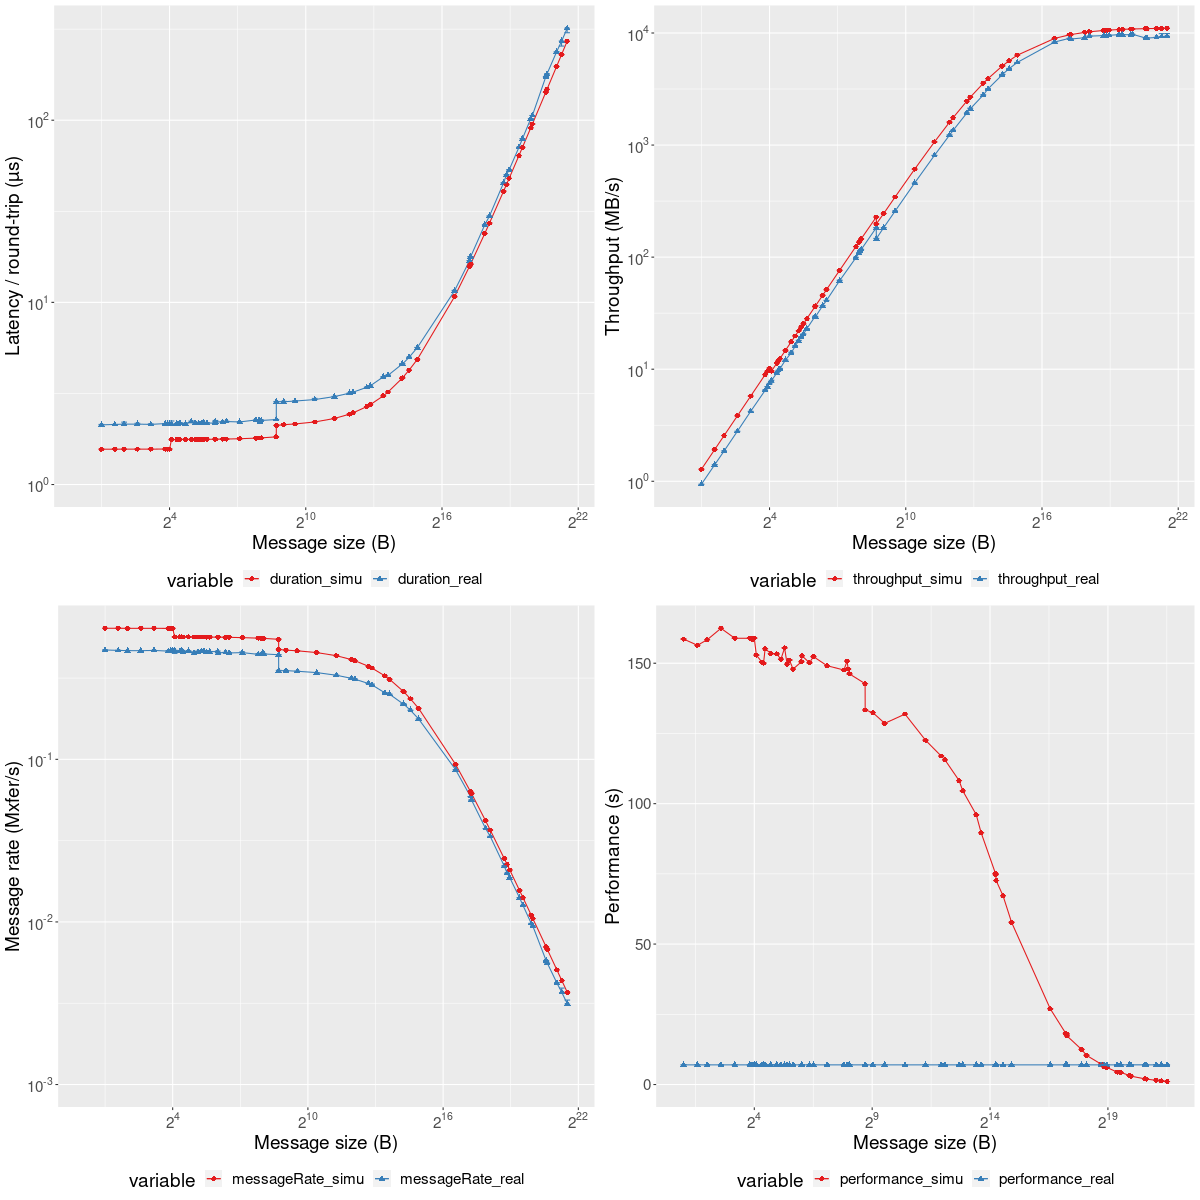
\includegraphics[width=\textwidth]{4_portals/ptlperf/ct.png}
    \caption{PtlPerf results for CT mode}
    \label{fig:4_portals:ptlperf_ct}
\end{figure}

\begin{figure}[!ht]
    \centering
    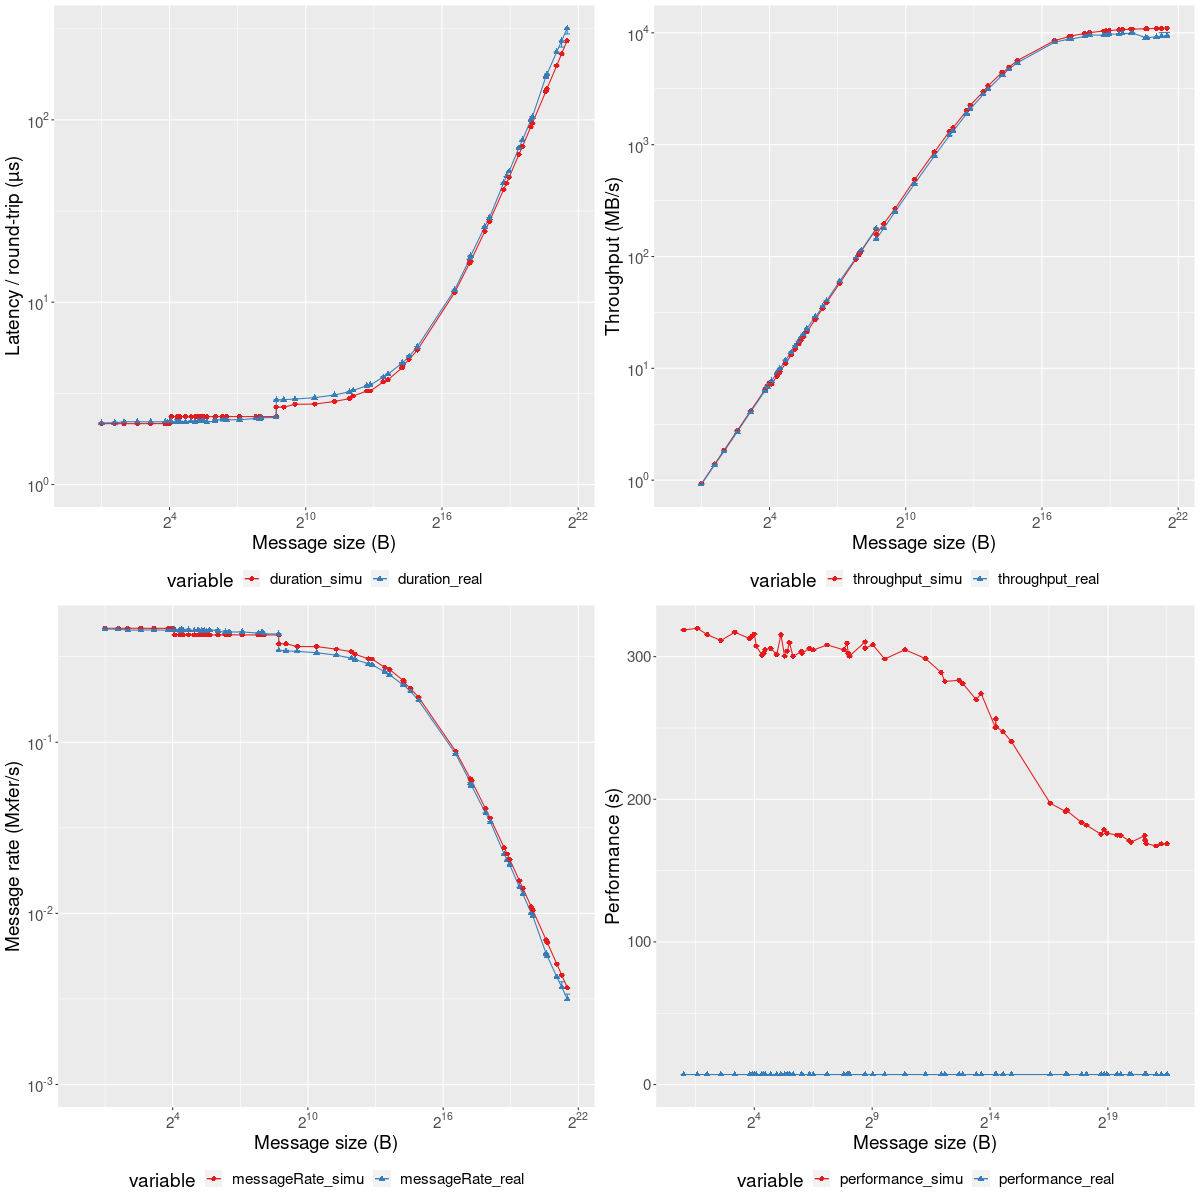
\includegraphics[width=\textwidth]{4_portals/ptlperf/ack.png}
    \caption{PtlPerf results for ACK mode}
    \label{fig:4_portals:ptlperf_ack}
\end{figure}

\begin{figure}[!p]
    \centering
    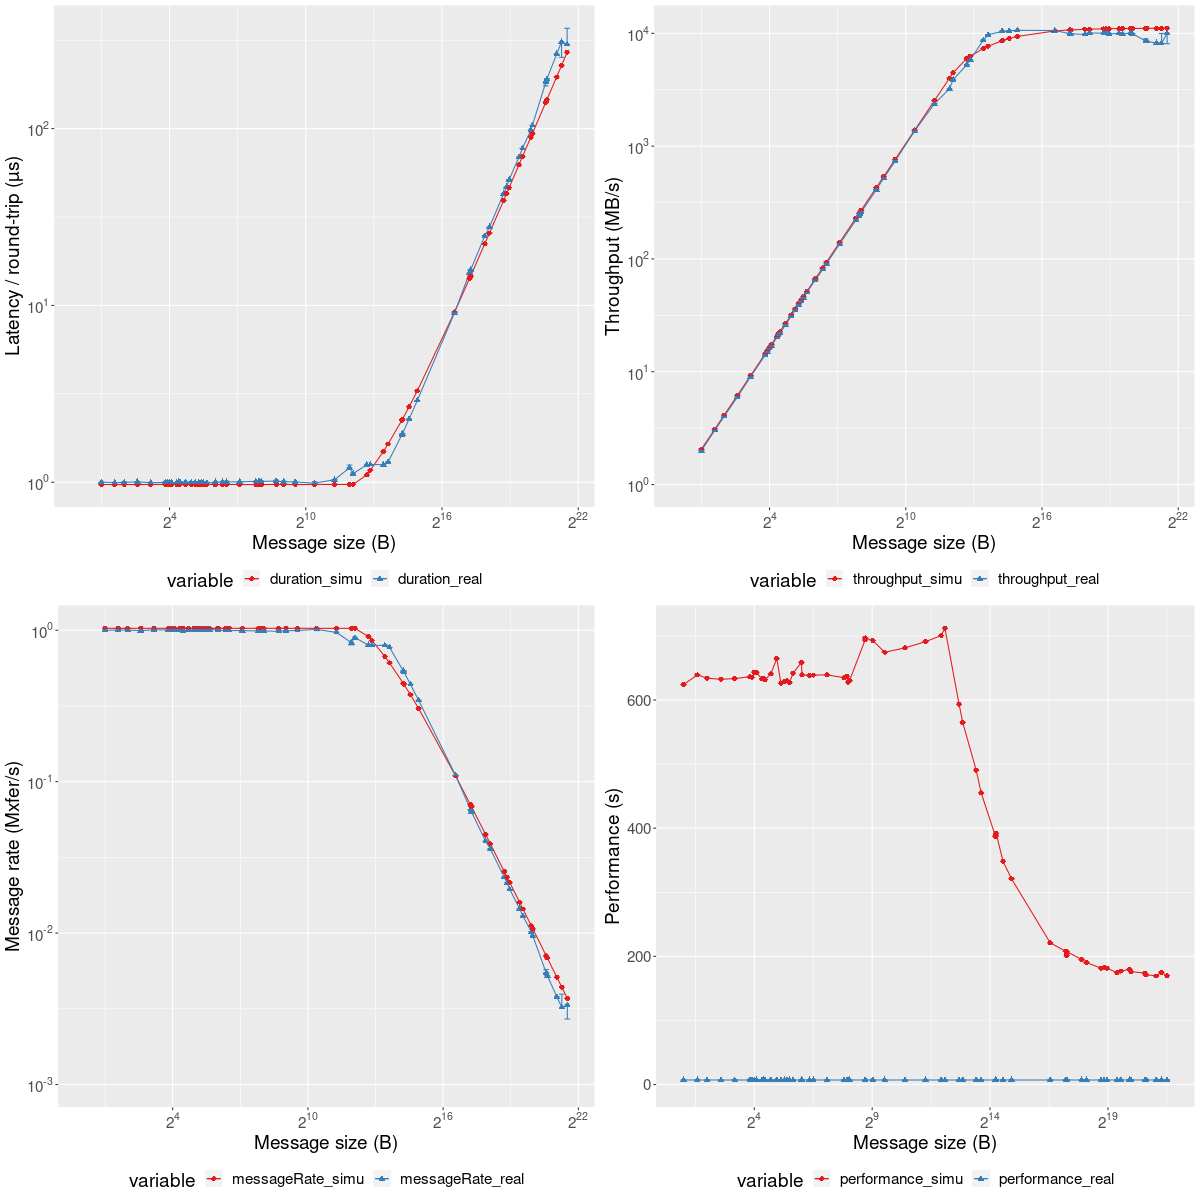
\includegraphics[width=\textwidth]{4_portals/ptlperf/match.png}
    \caption{PtlPerf results for match mode}
    \label{fig:4_portals:ptlperf_match}
\end{figure}

\begin{figure}[!p]
    \centering
    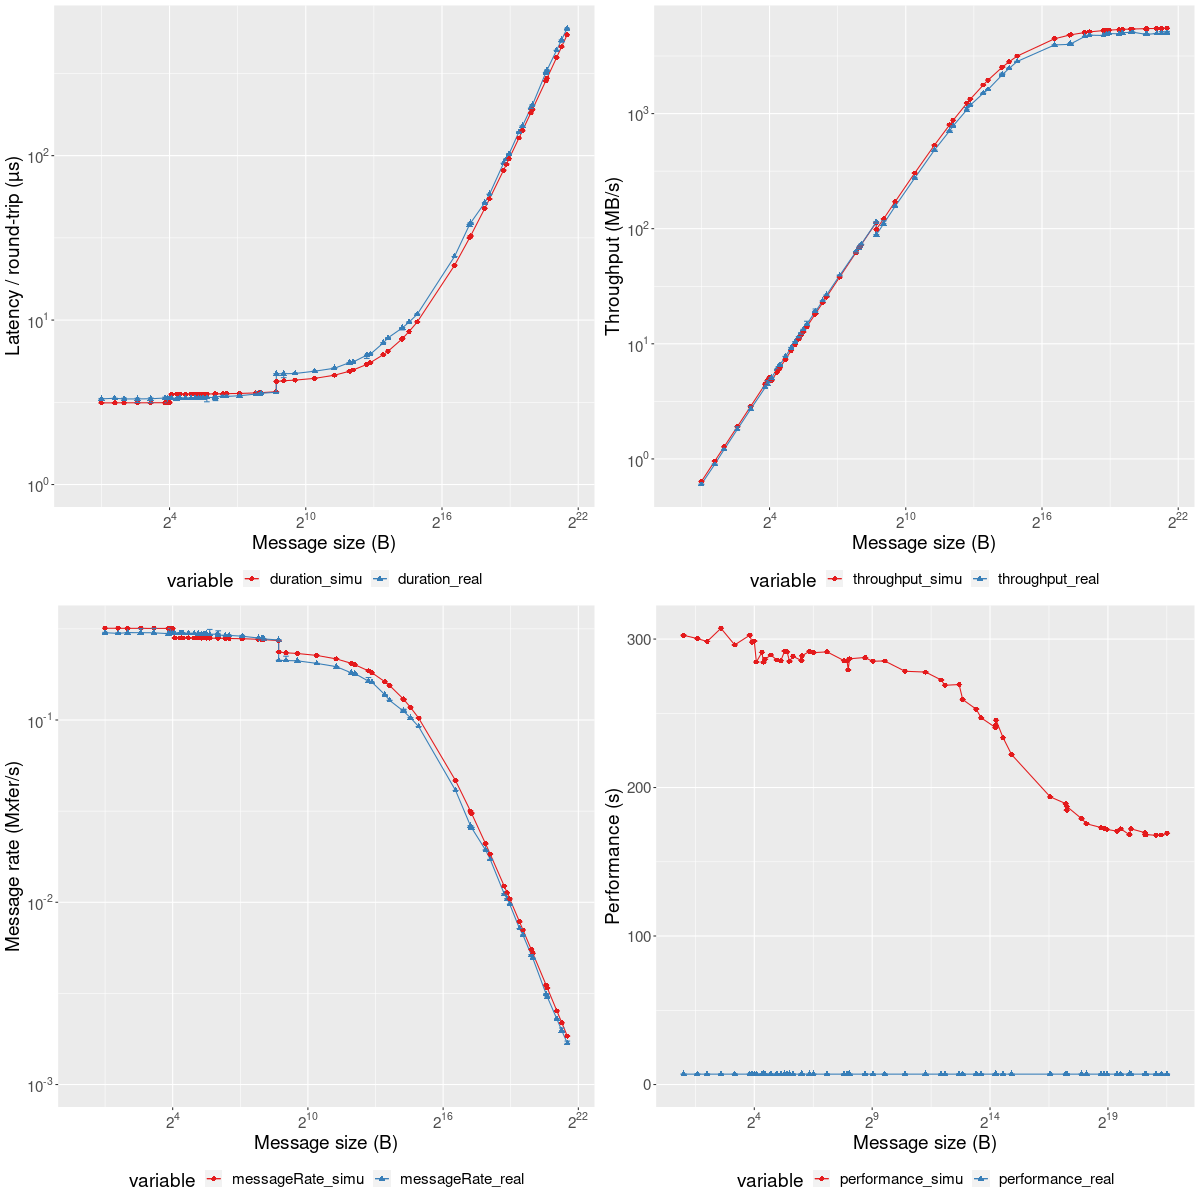
\includegraphics[width=\textwidth]{4_portals/ptlperf/reply.png}
    \caption{PtlPerf results for reply mode}
    \label{fig:4_portals:ptlperf_reply}
\end{figure}

Unlike our previous tests, which measure the time needed to send a fixed number
of messages, PtlPerf counts how many messages can be sent in a fixed amount of
time (using the \inline{PtlPut} primitive), and reports various statistics about the
transmissions (as presented in Section~\ref{subsubsec:2_context_hpc:ptlperf}).
While it offers many modes and options, we ran it in CT
(Figure~\ref{fig:4_portals:ptlperf_ct}), ACK
(Figure~\ref{fig:4_portals:ptlperf_ack}), match
(Figure~\ref{fig:4_portals:ptlperf_match}) and reply
(Figure~\ref{fig:4_portals:ptlperf_reply}) mode, for which the latency,
throughput, message rate, and performance of the simulator (in wallclock time)
compared to the real world execution are shown in the respective figures. CT,
ACK and reply mode all use one message inflight, as they are only meaningful in
this configuration, while for match mode we used the default limit on inflight
messages, which is 256.

We can see that ACK, match and reply modes have an excellent accuracy, and that
CT mode is acceptable even though it is not as perfect. From a performance point
of view, on all graphs we can see that larger messages cause the simulations to
be faster. This observation is expected, since in simulation no data is actually
transferred on a network, therefore modeling messages of all sizes has a similar
performance (no matter by how much the simulated time is increased, the
operation takes a constant amount of wall-clock time). Additionally, modeling
larger messages has an advantage for ptlperf in particular: since this benchmark
counts the number of messages sent in five seconds, instead of timing a fixed
number of iterations, it is expected that fewer operations will be performed
when larger messages are used, as each transfer takes more simulated time. 

We can also see that the performance of CT mode is much better than the other
ones, as it is the only benchmark which manages to be faster in simulation than
the real execution (for the biggest message sizes that we tested). The
explanation for this phenomenon comes from the way events are handled in
PtlPerf's code: after sending a message, the CT benchmark waits for the
completion of the communication using the \inline{PtlCTWait} primitive on a
counter. In simulation, this has the effect of putting the corresponding Actor
to sleep until the value of the counter is incremented, which is implemented in
an optimized way in our simulator. On the other hand, the other modes use full
events instead of counters, and instead of doing a \inline{PtlEQWait} in order
to wait for the completion of requests, they poll on the non-blocking
\inline{PtlEQGet} function between communications. In simulation, this has a
very negative effect on performance, because each polling loop only progresses
the simulated time by a very small amount, therefore the simulator will schedule
the polling Actor thousands of times before anything meaningful happens (like
receiving the event that is awaited), which is obviously very detrimental to
performance. This is a fundamental issue that is common in most Discrete Event
Simulators, and which we will discuss in more detail in the next chapter,
because we will see that it is particularly problematic in MPI (in
Section~\ref{subsec:5_high_level:polling}).


\chapter{Usage with high-level APIs}
\label{chap:high_level}

In our journey towards accurate simulation of HPC applications, we now have a
Portals simulator that we validated on point-to-point benchmarks. The next step
is then to run high-level APIs (such as MPI or OpenSHMEM) on top of S4BXI, since
real world applications and benchmarks are not usually written using low-level
APIs directly. In this PhD we will focus on the study of MPI, and in particular
Atos's implementation of this API, which is a fork based on OpenMPI which adds a
transport (called BTL for Byte Transfer Layer) optimized for BXI. We will also
show some results with OpenSHMEM on top of our simulator, even though we did not
go as much in depth because MPI is more commonly used with BXI in real world
scenarios.

\section{HPC software stack overview}

\begin{figure}[!b]
    \centering
    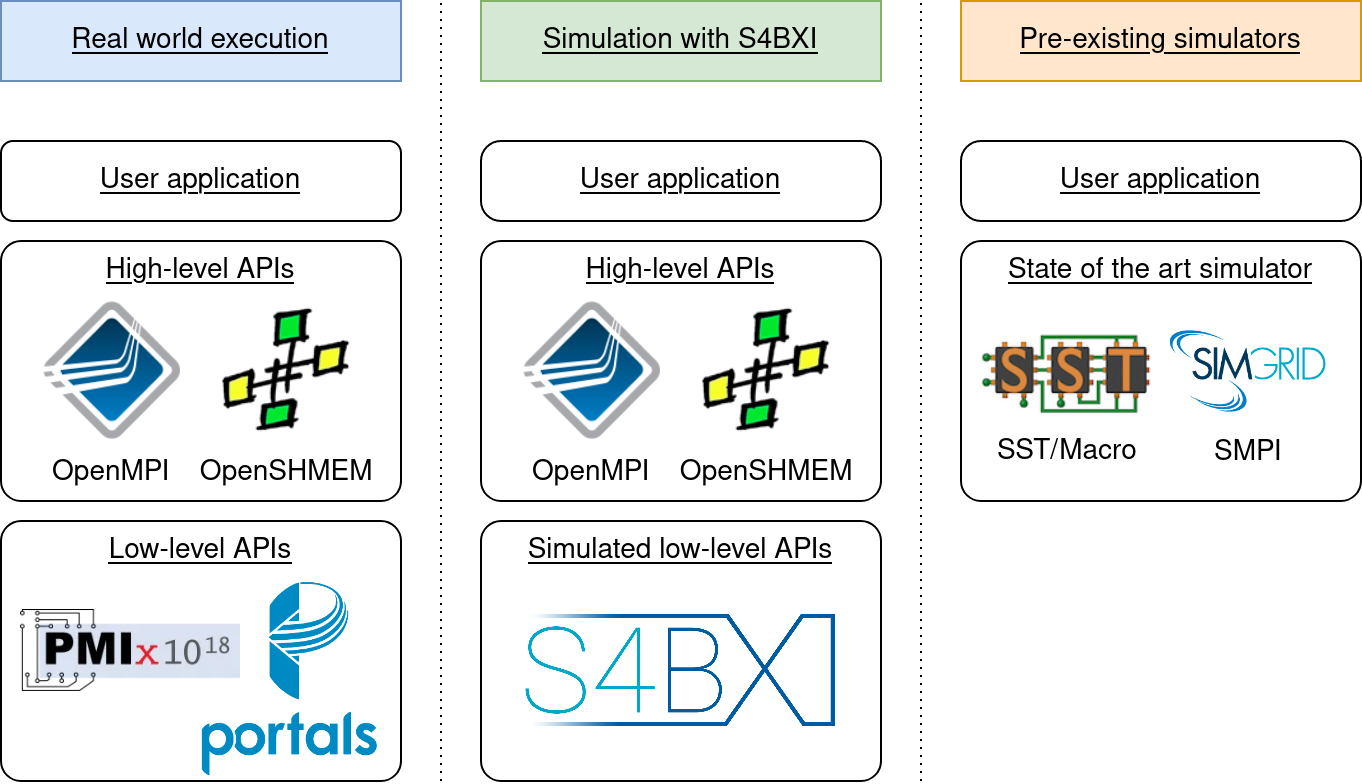
\includegraphics[width=1\textwidth]{5_high_level/software_sandwich.png}
    \caption{Software stack comparison: real world execution, S4BXI simulation and pre-existing state-of-the-art simulators}
    \label{fig:5_high_level:software_sandwich}
\end{figure}

As introduced in Section~\ref{subsec:2_context_hpc:software_stack}, a typical
software stack in HPC is made of several layers. Even though we have seen that
there are multiple possible combinations of these layers, in this section we
will focus on applications that are written directly on top of a high-level API
(in particular OpenMPI or OpenSHMEM), which uses Portals as a transport layer.
It is important to note that even though Portals is the low-level API used for
high-speed communications, high-level APIs also rely on communications across an
out-of-band network in order to initialize: indeed, it is often more convenient
to have access to a simple Ethernet network in order to exchange metadata that
will be used to set up the high-speed network. This is why high-level APIs also
use libraries such as the Process Management Interface (PMIx) for their
initialization, as they make the exchange of metadata across an out-of-band
network easier by providing primitives to perform barriers and basic data
exchanges. This software stack is represented on the left side of
Figure~\ref{fig:5_high_level:software_sandwich}.

The way this type of software stack is traditionally modeled is by intercepting
function calls at a high-level, and implementing full APIs such as MPI in
simulation directly. This is the approach which is used by state-of-the-art
simulators such as SST/Macro and SMPI, which is represented on the right side of
Figure~\ref{fig:5_high_level:software_sandwich}.

In comparison, our approach is to intercept communication primitives at Portals
level, in order to run unmodified high-level APIs on top of S4BXI, as
represented in the middle of Figure~\ref{fig:5_high_level:software_sandwich}.
There are several advantages to this approach: from a software development
perspective, implementing Portals in simulation is faster than re-implementing
all of MPI, since Portals only features point-to-point communications, whereas
MPI offers a wide range of two-sided and one-sided (RDMA) primitives, both
point-to-point and collective. Another advantage is that it allows running
different high-level APIs with a reasonable development effort, instead of
re-implementing fully every high-level API (as we will see with our OpenSHMEM
experiments, even though the majority of our work is focused on MPI). On the
other hand, there are also downsides to this approach: by running more software
layers in simulation, we expect the performance of the simulator to be worse
than higher-level models. There is also a more technical difficulty: in this
case, our low-level simulator implements Portals but we do not have a model for
PMIx (or the out-of-band network at all for that matters), which will complicate
the initialization of the high-level APIs.

The principle of our approach is to intercept communication primitives at an unusually low level in the software
stack. This method is not new and \cite{Knight2018} already implemented a similar concept, but
it has never been applied to either OpenMPI or Portals. We will see in the
upcoming sections that the technical solutions that we chose to work around the
difficulties of this approach are different from the previous approach.

\section{Atos's version of OpenMPI}
\label{sec:5_high_level:atos_ompi}

As explained previously, the most common API used on top of the BXI interconnect
is MPI, and in particular Atos's variant of OpenMPI, which we study in detail in
this PhD. While OpenMPI is a very complex set of libraries with many features,
we focus on the components that are used with BXI, which are represented in
Figure~\ref{fig:5_high_level:ompi_components}.

\begin{figure}[!ht]
    \centering
    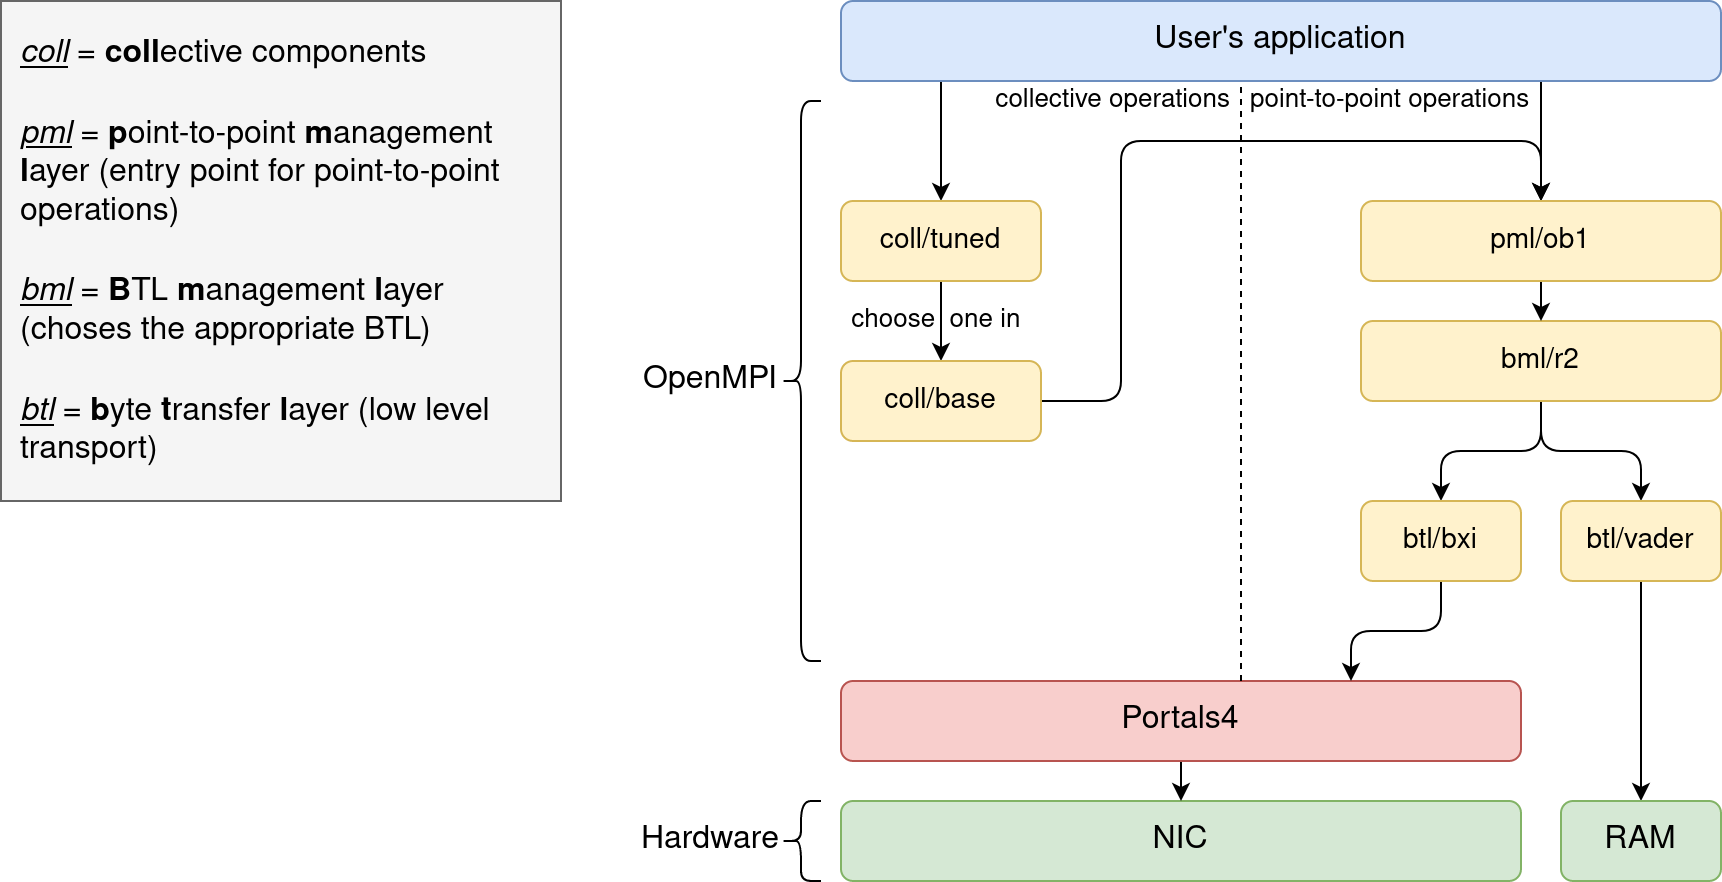
\includegraphics[width=1\textwidth]{5_high_level/ompi_components.png}
    \caption{Relevant OpenMPI components when using BXI}
    \label{fig:5_high_level:ompi_components}
\end{figure}

The components can be categorized in two main groups: collective and
point-to-point operations. Unlike Portals, MPI offers abstractions to perform
complex operations involving many processes (called ``ranks'' in MPI
vocabulary), without having the user worry about implementation details. These
operations are very diverse, such as ``gather'' (N to 1 communication),
``broadcast'' (1 to N), ``alltoall'', ``barrier'', etc. These operations all
have a synchronous and asynchronous variant, to allow users' application to
perform computations while the operation is progressing. To achieve that, the
\inline{coll/base} component implements several algorithms that perform any
given operation with a combination of point-to-point transfers (between only two
processes). Examples of a few algorithms for the broadcast operations are
displayed on Figure~\ref{fig:5_high_level:bcast_algos}, where each arrow
represents a point-to-point communication.

\begin{figure}[!ht]
    \centering
    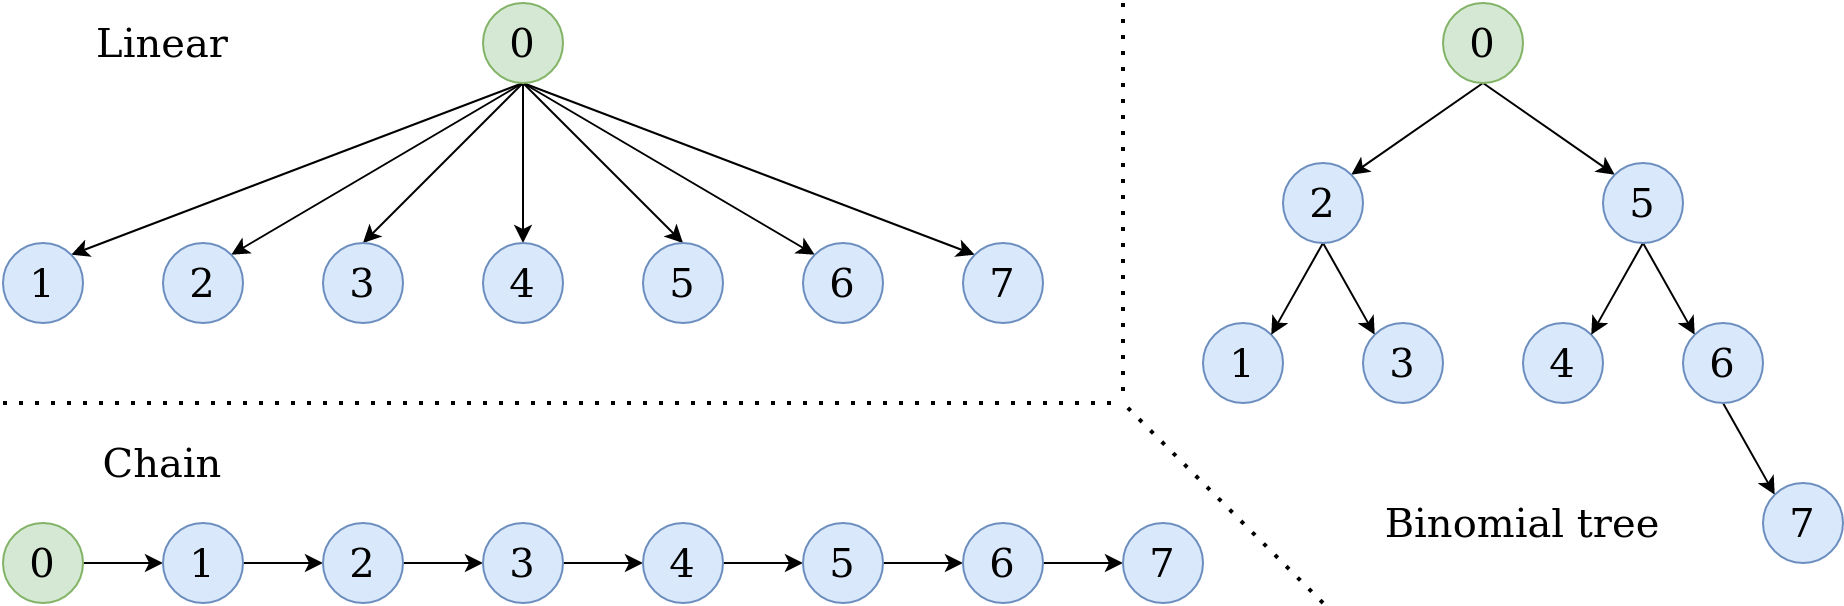
\includegraphics[width=1\textwidth]{5_high_level/bcast_algos.png}
    \caption{A few algorithm examples to perform a broadcast on 8 ranks from rank 0}
    \label{fig:5_high_level:bcast_algos}
\end{figure}

The reason different algorithms exist for each operation is to improve
performance: when the user calls a collective primitive, the
\inline{coll/tuned} component selects the algorithm to use in
\inline{coll/base} based on the number of ranks involved and the message
size. It is important to note that in the community version of OpenMPI, this
algorithm selection is based on benchmarks performed on old generation
Infiniband hardware, which is why teams at Atos made their own benchmarking
tools to optimize the algorithm choices for the BXI interconnect. Therefore,
the algorithms used in Atos's version of OpenMPI are not the same as in the
community version of OpenMPI, and still evolving (as this optimization work is
not finished as of the writing of this PhD).

When performing point-to-point operations (either from user code or as part of a
collective operation), there are three types of components that will be of
interest to us: at the highest level, the PML (Point-to-point Management Layer)
is responsible for any manipulation of the data that might be required, such as
the fragmentation of large messages. In Atos's OpenMPI the PML that we use is
called \inline{ob1} and it is not modified from the community one. Then the BML
(BTL management layer) chooses which BTL can perform the communication, based on
the location of the two ranks involved (they could run on the same machine, or
be on different nodes). The BML that we use is called \inline{r2} and it is also
identical to the community one. Finally, the BTL (Byte Transfer Layer) performs
the low-level transfer. Usually several BTLs will be used, as we can see on
Figure~\ref{fig:5_high_level:ompi_components}: for example, with the BXI
interconnect the \inline{btl/bxi} component will be used to perform
communications across the high-speed network, but the \inline{btl/vader} will be
used to perform shared memory transfers for ranks that are on the same machine.
Vader is a BTL that also comes unmodified from the community version of OpenMPI,
and BXI is entirely made by teams at Atos.

\section{Adapting OpenMPI for the simulated world}

\subsection{Simulation of out-of-band communications without PMIx}

As introduced in the previous section, the main difficulty in running a real
world MPI implementation in our simulator is the initialization: it requires
either to implement the PMIx specification in simulation, or to modify MPI
itself in order not to need this library. There are pros and cons to both
options: implementing PMIx allows running MPI with very few modifications, and
also facilitates running other high-level APIs (since PMIx is a tool commonly
used by several libraries). On the other hand, developing and maintaining a PMIx
simulator represents significant work, as it has many features. It is worth
noting that regardless of the option we choose, the accuracy of the simulator
will not be affected too much, since PMIx is only used briefly at the start and
at the end of the execution of applications. In either case we will also likely
need to rebuild MPI for simulation, since our simulator requires MPI to be built
with a specific set of options (passed to the \inline{configure} script) that
are likely different from a production build for real world executions (in
particular, we need to force OpenMPI to build into only three shared libraries,
instead of one library for each component). In the case of running Atos's
OpenMPI on top of S4BXI, we chose to add a small patch to MPI instead of
implementing PMIx, for all the reasons mentioned above. In particular, we
believe that this patch is easier to maintain than a full PMIx implementation,
and we will see in the next sections that other small modifications to MPI's
code will prove useful. A summary of the different software layers involved in
the execution of an MPI application is depicted in
Figure~\ref{fig:5_high_level:models_comparison}.

\begin{figure}[!ht]
    \centering
    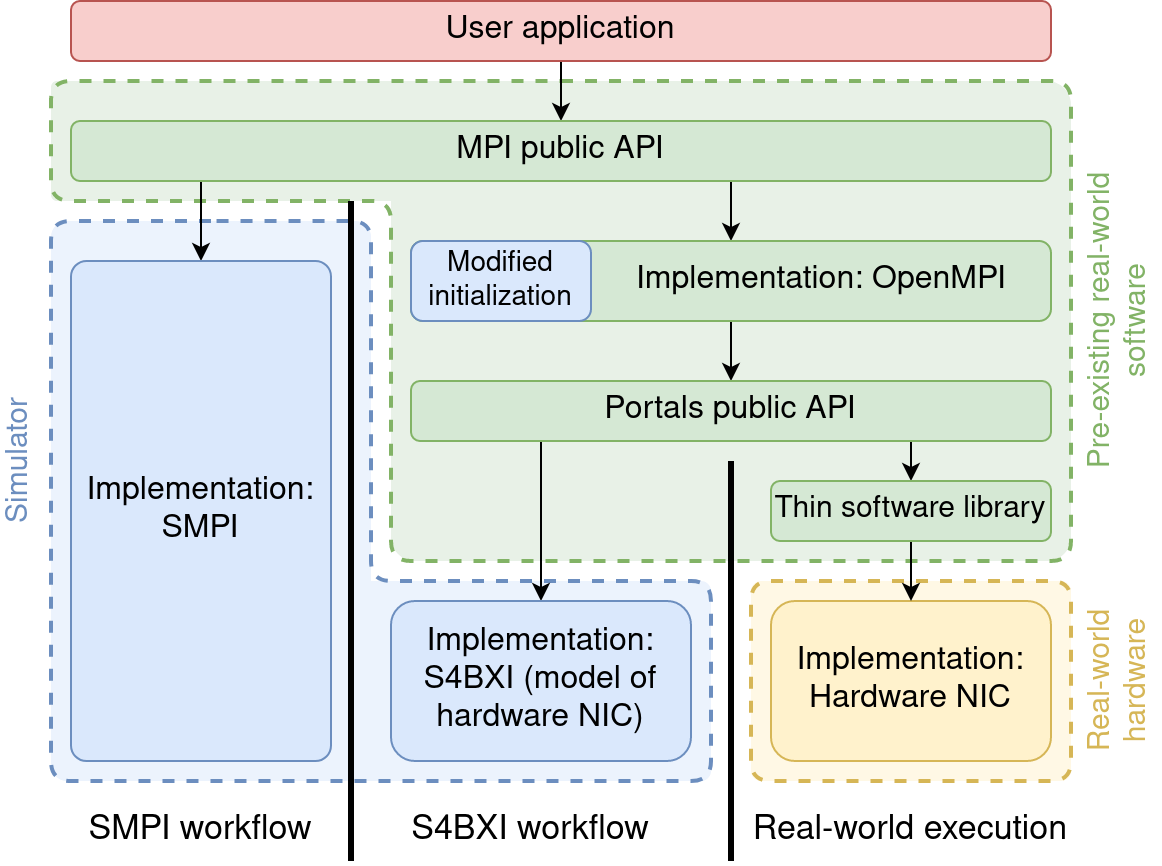
\includegraphics[width=0.8\textwidth]{5_high_level/model_comparison.png}
    \caption{Software layers involved in state of the art simulation, S4BXI simulation, and real-world execution of MPI applications}
    \label{fig:5_high_level:models_comparison}
\end{figure}

In total, our patch modifies 345 lines of code of OpenMPI: 41 lines are added,
224 are removed, and 80 are modified. This number is very small compared to the
size of the OpenMPI codebase, which contains nearly 900 thousand lines of code.
The detail of these statistics language by language are available in
Appendix~\ref{app:ompi_patch}. We also know from a year of maintaining our patch
that the code that we modified is not updated very often, as we were able to
rebase our modifications on top of the latest development to OpenMPI through
seven versions (from version 4.0.4 to 4.1.4), without any major difficulty (the
rebase through git worked automatically in the vast majority of cases). The next
sections give more detail about the components that are modified by this patch.

\subsection{Adapting OpenMPI's initialization for S4BXI}

Our patch to OpenMPI affects two main components: the initialization of MPI
itself (globally), and the initialization of the BTLs. The impacted components
are shown in Figure~\ref{fig:5_high_level:simplified_arch}.

\begin{figure}[!ht]
    \centering
    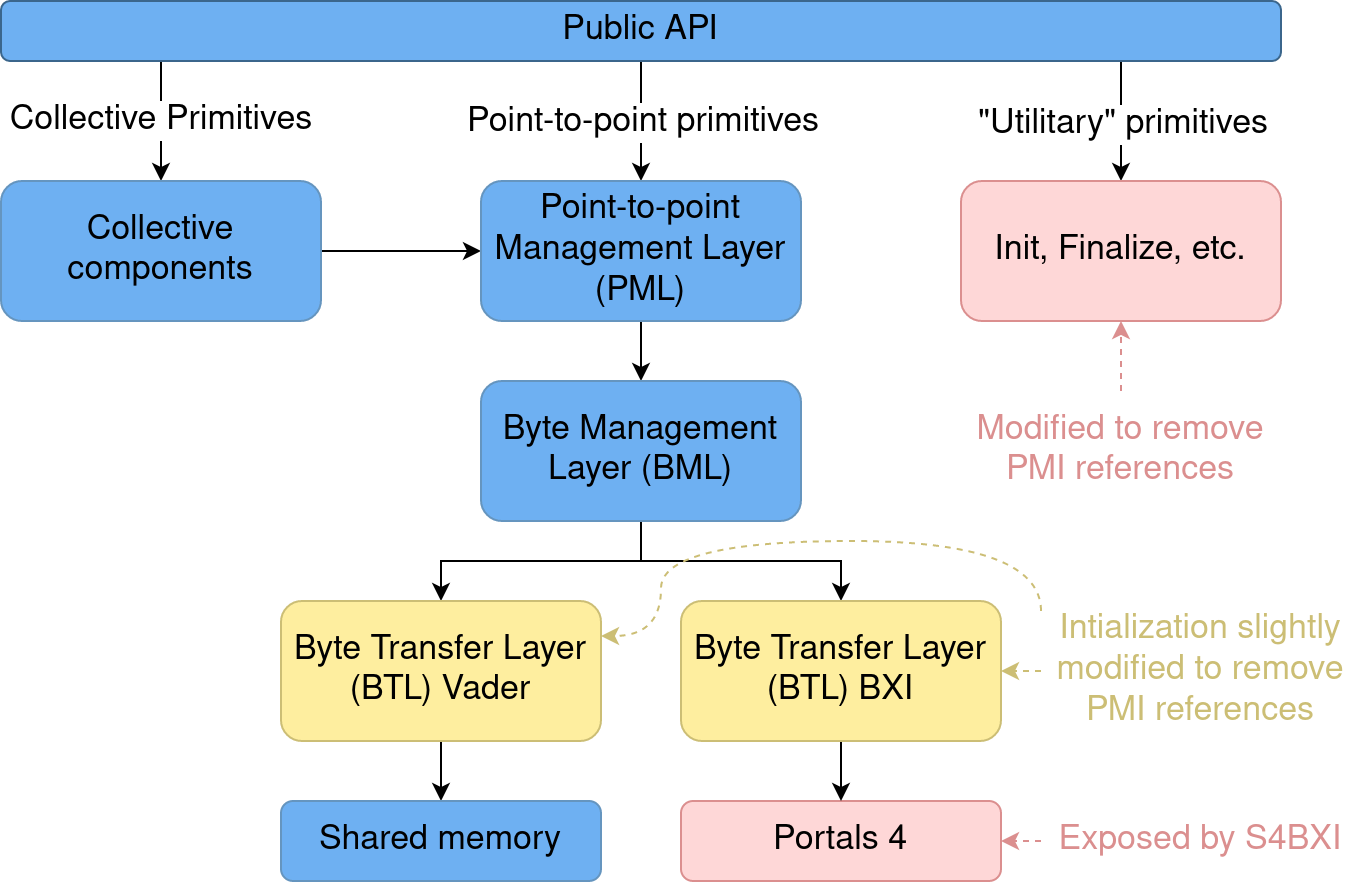
\includegraphics[width=0.75\textwidth]{5_high_level/simplified_arch.png}
    \caption{MPI components impacted by our patch \small{(dark blue is unmodified, medium yellow corresponds to minor modifications, and light red is heavily modified)}}
    \label{fig:5_high_level:simplified_arch}
\end{figure}

In the initialization of OpenMPI, we mainly replace PMIx calls to functions
native from our simulator in order to give all processes the knowledge of what
their rank is, how many processes are involved in the current job, and which
other ranks are local to the same machine. Additionally, there are a few
barriers between all the ranks that are reimplemented with SimGrid's built-in
Barrier object instead of using PMIx. An example of such replacement is shown on
Figure~\ref{fig:5_high_level:ompi_example_diff}: below several layers of macros,
\mbox{\inline{OPAL_MODEX_*}} calls use PMIx to exchange data with other
processes, so we replace them by simple function calls to our simulator which
fetch the equivalent data in the simulated world. In this specific example, the
call returns a Portals process structure (which includes a NID and a PID) for
the requested MPI rank (which correspond to the \inline{vpid} attribute
internally in OpenMPI), which is used to initialize the \inline{btl/bxi}
component.

\begin{figure}[!ht]
    \lstinputlisting[basicstyle=\ttfamily\small,frame=bt,language=diff]{5_high_level/ompi_example.diff}
    \caption{Example section of our patch to OpenMPI}
    \label{fig:5_high_level:ompi_example_diff}
\end{figure}

In the BXI BTL, the data that is exchanged at startup is mainly the Portals IDs
of each process, in particular the NIDs of all the processes involved in the
current job. At startup, the BTL also looks for all available NICs in Sysfs (in
the \inline{/sys/class/bxi} virtual folder), in order to use the closest one (in
the case of a NUMA machine). This processing had to be removed for simulation at
first, since on the host running the simulation, any BXI NIC physically present
on the machine does not correspond to the hardware simulated by our model in the
virtual world. Since then, the MPI team at Atos has been kind enough to add an
option in MPI to disable this optimization (and therefore use any available NIC
without asking for a particular location), which allows our patch to be even
lighter since we do not need to hardcode the removal of this feature.

\subsection{Shared memory support}
\label{sec:5_high_level:shared_mem_support}

As presented in Section~\ref{sec:5_high_level:atos_ompi}, MPI supports using
several BTLs for point-to-point communications. In the case of BXI clusters,
most of the time two BTLs will be used: BXI for communications on the high-speed
network, and Vader for intra-node communications using shared memory (when
several MPI ranks are executed on the same machine).

In order to support Vader in simulation, we also modified its initialization. It
is not strictly necessary in order to perform simulations of MPI (we could have
simply disabled Vader altogether), since communications between two ranks on the
same machine can still be performed trough BXI: in that case messages just go
back and forth on the PCIe bus without being sent on the network (both in a real
execution and in simulation). Nevertheless, we added support for Vader in order
to allow users to replicate their real-world scenario as closely as possible in
simulation. In theory this BTL is easy to initialize, and does not require any
data from the simulator, but in practice there is a different kind of issue with
the modeling of this BTL in simulation: by default, the name given to the files
which hold data in shared memory (in the \inline{/dev/shm} folder) can be
identical on different machines. In a real-world execution this does not matter,
as each machine will hold its own set of files, but in simulation all ranks run
on the same physical machine (which executes the simulation), which means that
different simulated processes could overwrite the data of processes on different
simulated nodes. Therefore, we had to make the name of these files unique across
the whole simulation, which required a small modification of Vader's
initialization. It is worth noting that this modification is not related to
PMIx, and therefore it further justifies our choice to patch MPI instead of
reimplementing PMIx in simulation, as this part of the patch would have been
required in any case.

\subsection{Handling copies of MPI libraries in S4BXI}
\label{sec:5_high_level:relinkage_of_libs}

Up to this point, the simple applications that we modeled did not have any
dependencies on external libraries, except Portals which is directly provided by
our simulator. Now that we try to model MPI, we face a new difficulty: as
explained in Section~\ref{subsec:4_portals:process_isolation}, we rely heavily
on the linker to isolate the global symbols of the user application in each
simulated process, but we do not have a way of isolating different copies of
external libraries (such as OpenMPI) yet. This is problematic because OpenMPI
relies heavily on global variables, which need to be ``private'' to each
simulated process. In order to tackle this issue, we can take inspiration from
SMPI: the same way that it copies the user application $N$ times (for $N$
simulated processes) in order to isolate them, it also has an option to make
multiple copies of any linked library, and then ``re-link'' the copies of the
user application and the libraries together (the current proof-of-concept
implementation uses a somewhat brutal \inline{sed} command in the copied user
applications directly). In the end, each simulated process has its own copy of
the user application, which is linked with its own copy of any library that
needs to be ``privatized'', as depicted in
Figure~\ref{fig:5_high_level:smpi_relinkage}.

\begin{figure}[!ht]
    \centering
    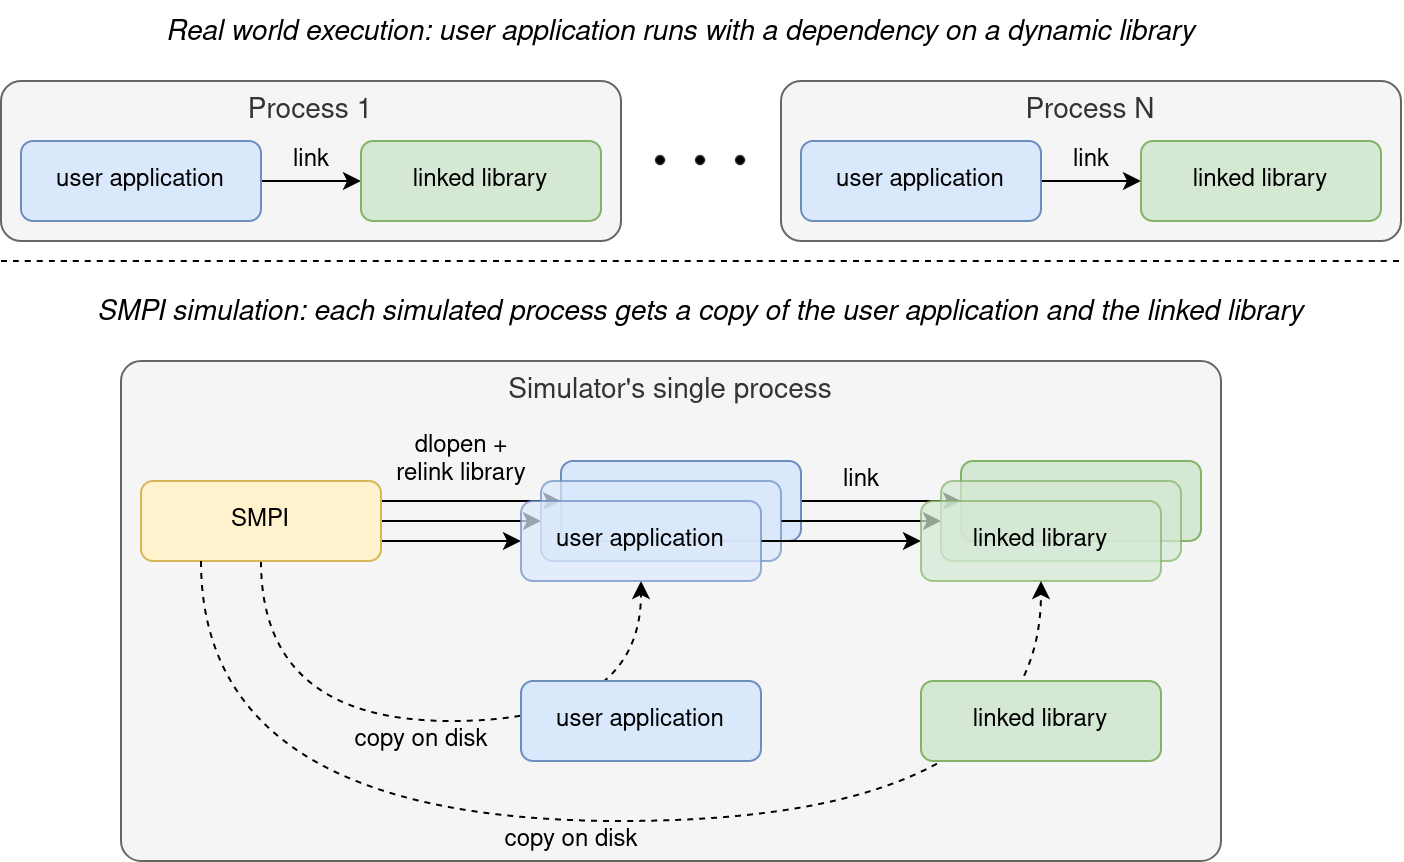
\includegraphics[width=1\textwidth]{5_high_level/smpi_relinkage.png}
    \caption{Methodology to ``privatize'' libraries in SMPI, compared to the real-world execution}
    \label{fig:5_high_level:smpi_relinkage}
\end{figure}

While this works well for libraries that are self-contained, we encountered an
issue when trying this methodology with MPI: OpenMPI does not consist of just
one library, but of three libraries (called OMPI, OPAL and ORTE), which are all
linked to the user application, but also linked to each other. Therefore, in
order for this ``privatization'' to work, we had to extend it in order to relink
not just the user application to each library, but also the copies of each
library together. This extended approach that we implemented in S4BXI is
depicted in Figure~\ref{fig:5_high_level:ompi_relinkage}.

\begin{figure}[!ht]
    \centering
    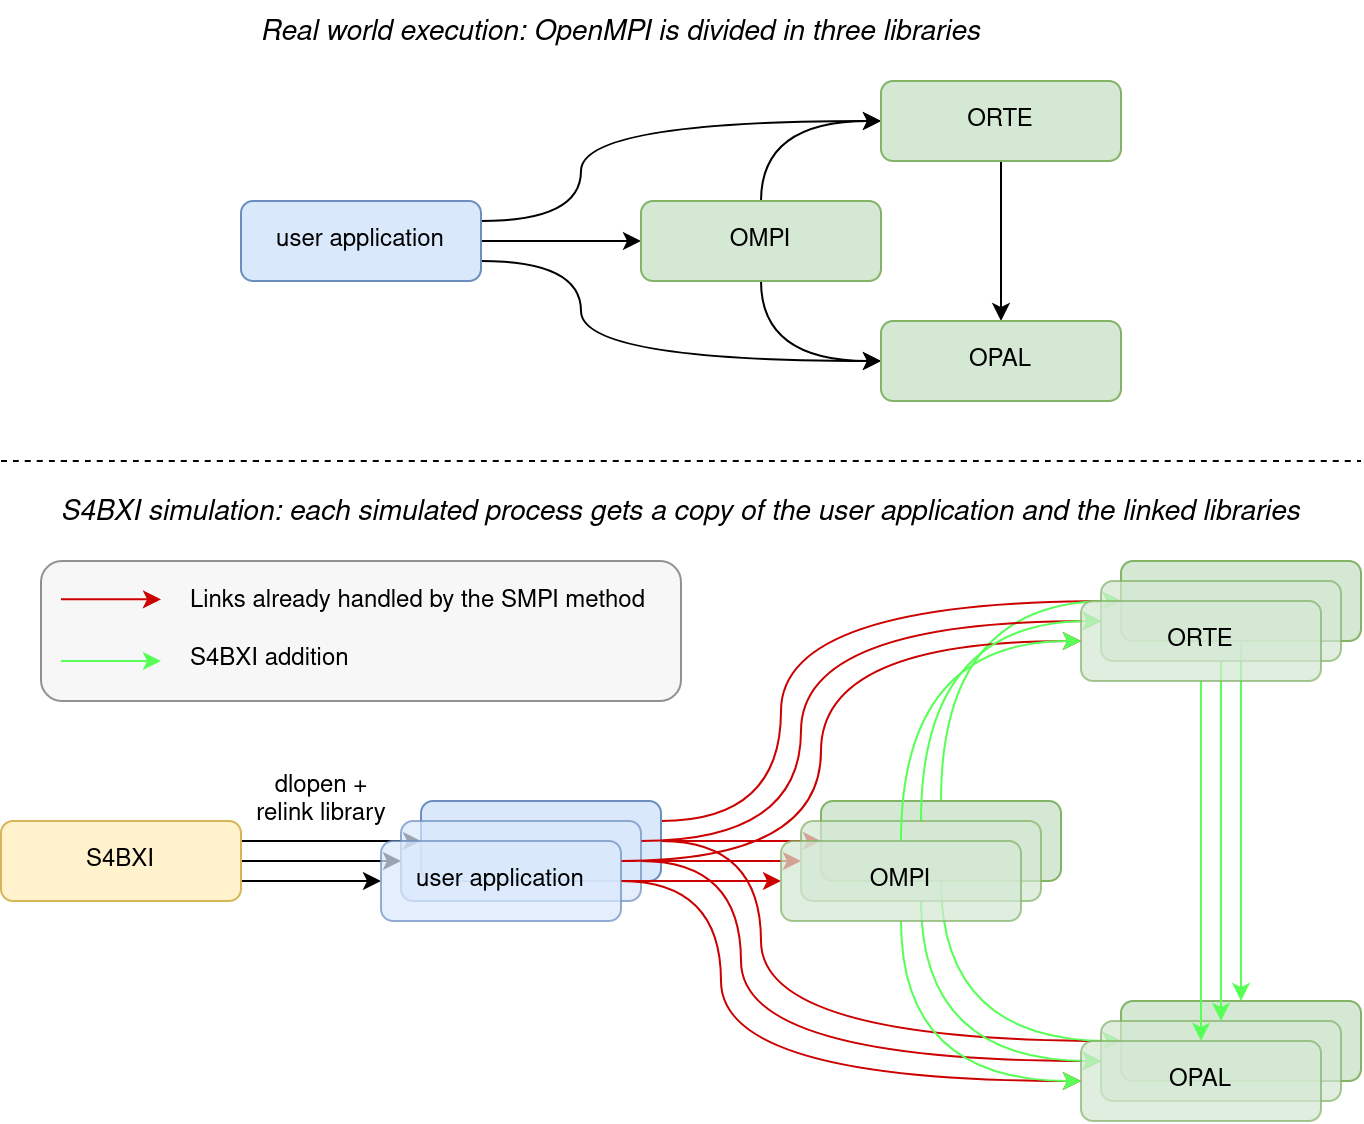
\includegraphics[width=1\textwidth]{5_high_level/ompi_relinkage.png}
    \caption{Methodology to ``privatize'' OpenMPI libraries in S4BXI, compared to the real-world execution (the ``copy on disk'' step is still present but not depicted for clarity)}
    \label{fig:5_high_level:ompi_relinkage}
\end{figure}

\subsection{A word on performance regarding polling}
\label{subsec:5_high_level:polling}

Thanks to our patch to OpenMPI, we can run simulations of real-world
applications on top of our simulator. However, we still face an issue when it
comes to performance, because of a fundamental problem with discrete event
simulators: polling. This issue was already mentioned in
Section~\ref{sec:4_portals:ptlperf}, as we observed that it impacted greatly the
performance of Ptlperf's simulations, but it is really with MPI that this
problem is the most noticeable.

In simulation, we have two different ``times'': ``wall-clock time'', during
which the user waits for the simulation to finish, and ``virtual time'', which
is a variable inside SimGrid used to keep track of the time in the simulated
world. On the other hand, on a real cluster executing a scientific application,
there is only one time: the makespan of the application. This difference becomes
very important if an application performs polling, i.e. loops over a check until
it completes. In the real world, performing polling or a ``passive'' wait is
equivalent if nothing else is running on the same CPU core. An example is
depicted on Figure~\ref{fig:5_high_level:wait_example}: while both solutions
would take the same amount of time in a real-world execution, these two programs
have a very different simulation performance.

\begin{figure}
    \centering
    \begin{subfigure}{.5\textwidth}
        \centering
        \lstinputlisting[basicstyle=\ttfamily\scriptsize,frame=bt,language=C]{5_high_level/active_polling_example.c}
        \caption{Polling around EQ Get}
        \label{fig:5_high_level:active_polling_example}
    \end{subfigure}% this comment is important otherwise the figures are vertical
    \begin{subfigure}{.5\textwidth}
        \centering
        \lstinputlisting[basicstyle=\ttfamily\scriptsize,frame=bt,language=C]{5_high_level/passive_wait_example.c}
        \caption{Passive wait with EQ Wait}
        \label{fig:5_high_level:passive_wait_example}
    \end{subfigure}
    \caption{Two ways of waiting for an event in Portals}
    \label{fig:5_high_level:wait_example}
\end{figure}

The explanation is that \inline{PtlEQWait} is cleverly implemented in our
simulator, i.e. the Actor who calls the primitives is put to sleep until the
arrival of the awaited event. On the other hand, the active polling loop of
Figure~\ref{fig:5_high_level:active_polling_example} causes an issue, because
\inline{PtlEQGet} takes a small amount of wall-clock time to simulate, but it
doesn't allow the virtual simulated time to progress. This means that when an
Actor runs such a polling loop, it will be continuously scheduled to run by
SimGrid's scheduler, but the simulated time will never progress, effectively
resulting in a deadlock of the simulation (with respect to wall-clock time).

This is a significant issue, because OpenMPI relies on polling mechanisms every
time an application asks to wait for the completion of a request (in this
context a ``request'' is to be taken in a very broad way: it could represent a
message transmission, a message reception, a collective operation, etc.). It is
worth noting that this problem is not specific to OpenMPI over Portals, but is a
common problem in discrete event simulation: if we look at simulators which
operate one level of abstraction higher in the software stack, we can see the
same problems. For example, if an application calls the \inline{MPI_Test}
primitive in a loop (which is not uncommon), SMPI will suffer the same issue.
The way SMPI handles the problem is by injecting increasing amounts of delay in
the simulated time, in the form of a small CPU execution (which is purely
artificial and does not correspond to real computation).

\begin{algorithm}
    \caption{OpenMPI's algorithm to wait for the completion of a request}
    \hspace*{\algorithmicindent} \textbf{Input} $request$ a pending request, $BTL$ the list of BTLs in use, $N$ the number of BTLs
    \begin{algorithmic}[1]
    \While{$request$ is not complete}
        \For{$i \gets 0$ to $N - 1$}
            \State{progress\_btl\_number($i$)}
        \EndFor
    \EndWhile
    \end{algorithmic}
    \label{alg:5_high_level:ompi_wait}
\end{algorithm}
\begin{algorithm}
    \caption{Algorithm~\ref{alg:5_high_level:ompi_wait} applied to our specific case}
    \hspace*{\algorithmicindent} \textbf{Input} $request$ a pending request
    \begin{algorithmic}[1]
    \While{$request$ is not complete}
        \State{progress\_btl\_BXI()}
        \State{progress\_btl\_vader()}
    \EndWhile
    \end{algorithmic}
    \label{alg:5_high_level:ompi_wait_specific}
\end{algorithm}

Initially, we resolved this issue in our simulation with a better approach: by
analyzing the code of OpenMPI, we were able to find a heuristic to determine
when it was safe to perform a Portals EQ Wait (i.e. blocking wait) instead of a
loop over an EQ Get. This allowed us to keep an accurate simulation while
speeding it up by orders of magnitude. Unfortunately, this solution only worked
well at the time when we supported only the BXI BTL in simulation. Indeed,
internally the algorithm used to wait for the completion of a request roughly
follows Algorithm~\ref{alg:5_high_level:ompi_wait}, where the PML will loop over
each BTL and call its ``progress'' function until the request is complete. The
``progress' function of a BTL typically runs every callback that is ready in the
context of asynchronous operations, and checks for new events coming from the
underlying transport. When we supported only one BTL, it was easy to replace the
progress function by a blocking wait. Unfortunately, when we added support for
shared memory transfers using the vader BTL, this optimization stopped working,
because the completion of a request could now come from any of the two BTLs, as
depicted in Algorithm~\ref{alg:5_high_level:ompi_wait_specific}. In the general
case it is not possible to know from which BTL the completion of a request will
come, because of how generic a request is in this part of a code. Additionally,
our problem was further complicated by the fact that some options of OpenMPI
require progress functions to run as often as possible: for example, it is
possible to turn on flow control for the BXI BTL of OpenMPI, in which case if
too many messages are already inflight, new ones will wait in a queue (in order
not to flood a target). It is then in the progress function of the BXI BTL that
a check will be performed to see if pending messages can be sent. Therefore,
having a blocking wait in this function stops this check from working properly,
since it might get scheduled too late, or not at all in the worst situations.

This problem further reduces the number of cases in which our heuristic to
improve performance works, and therefore we abandoned it completely: in the
latest versions of our simulator, we implement the same mechanism as SMPI in
S4BXI, i.e. injecting growing amounts of delay inside \inline{PtlEQGet} to make
sure that a polling loop can still allow the simulated time to progress at a
reasonable rate (this small delay is configurable using the environment variable
\inline{S4BXI_ACTIVE_POLLING_DELAY}).

\section{Compatibility with SMPI sampling}

When running applications in simulation, one of the biggest concern is the
memory usage and the performance of the simulator: indeed, most simulators built
with SimGrid are single-threaded, which means that all processes of the
application end up being executed sequentially on one CPU core. To mitigate this
issue, SMPI offers a set of macros in order to replace some heavy computation
parts with increments in the simulated time. The amount of computation time to
inject can be statically provided by the user, or determined automatically at
runtime, thanks to macros which replace \inline{for} loops. These macros allow
SMPI to execute the first iterations of the loop in order to measure their
duration, and to replace the later ones with artificial computation time. For
memory usage, SMPI allows users to mark some memory allocation as ``shared'',
which means that all simulated process will use the same physical memory region
instead of all doing a new allocation. Of course this generally makes the result
of computations functionally wrong, but for applications in which the control
flow does not depend on the input data it is a good solution to run full size
applications in simulation and get good performance estimations. These macros
effectively allow users to make skeleton version of their application, in order
to speed up simulation and allow it to run on a single CPU.

In S4BXI, we are able to re-use all these SMPI macros transparently, since both
simulators are based on SimGrid. This allows us to re-use studies that have been
conducted on specific applications in order to create optimized skeleton
versions. For example, Tom \textsc{Cornebize}'s thesis~\cite{Cornebize2021}
studied HPL extensively, and we re-used his model of HPL's computation phases in
order to speed up S4BXI simulations by orders of magnitude. This will be
demonstrated in our validation experiments in
Section~\ref{sec:5_high_level:benchmarks}.

\section{Experimental validation}
\label{sec:5_high_level:benchmarks}

While most applications can be run using both MPI and OpenMP parallelization
(sometimes even CUDA), in our experiments we will distribute them using MPI
only, as our simulator does not support arbitrary OpenMP (nor CUDA) code. This
is a common limitation which is present in similar simulators as well (such as
SMPI for example). There is a priori no fundamental limitation that would
prevent us from developing a model for OpenMP or CUDA, but such a development is
way beyond the scope of this thesis.

We will start with OSU micro-benchmarks, which are a set of
very simplistic ``unit-style'' tests that benchmark a single primitive in a
loop. While the resulting workload is completely unrealistic, it is a common
tool to assess the performance of a cluster on a specific MPI primitive, and it
is also a good validation that all collective and point-to-point operations work
without errors in simulation. We will then study realistic applications that we
presented in Chapter~\ref{chap:biblio_simu}: LULESH, Quicksilver and HPL.

From a technical perspective, all our benchmarks will be executed on a
real-world cluster composed of nodes equipped with BXI v2 hardware and AMD EPYC™
7763 64-Core processors. In simulation, we will run each application both in our
model (with OpenMPI on top of S4BXI), and in SMPI, in order to compare our
approach to the closest state-of-the art simulator.

\subsection{OSU micro-benchmarks}
\label{subsubsec:5_high_level:osu_results}

For these experiments, we will run point-to-point benchmarks on two machines,
and collective operations on 16 machines, with only one process on each machine
in order to maximize the network load. Experiments were also performed on 32 MPI
ranks (8 nodes and 4 processes per node), but the conclusions where very
similar, therefore this data is only shown in Appendix~\ref{app:osu_32} to keep
this section more readable. The simulations are performed on one of the machines
from the real-world cluster, with an AMD EPYC™ 7763 64-Core processor (even
though only one core of the processor is used in each simulation). Since OSU
micro-benchmarks cover many MPI primitives, it is impractical to analyze the
result of each simulation exhaustively. Instead, we present a few significant
experiments, but we also show global statistics about all the simulations.

Across all benchmarks, we get mainly two types of results. In some cases, both
SMPI and OpenMPI over S4BXI give very good results (i.e. latencies reported by
the benchmark at the end of its execution). We can see  an example of such a
behavior with the AllGather benchmark, depicted on
Figure~\ref{fig:5_high_level:osu_allgather_16} (AllGather allows all processes
to send chunks from a local buffer to all the other processes in the job).

\newgeometry{top=2.2cm,footskip=0.8cm}
\begin{figure}[!p]
    \centering
    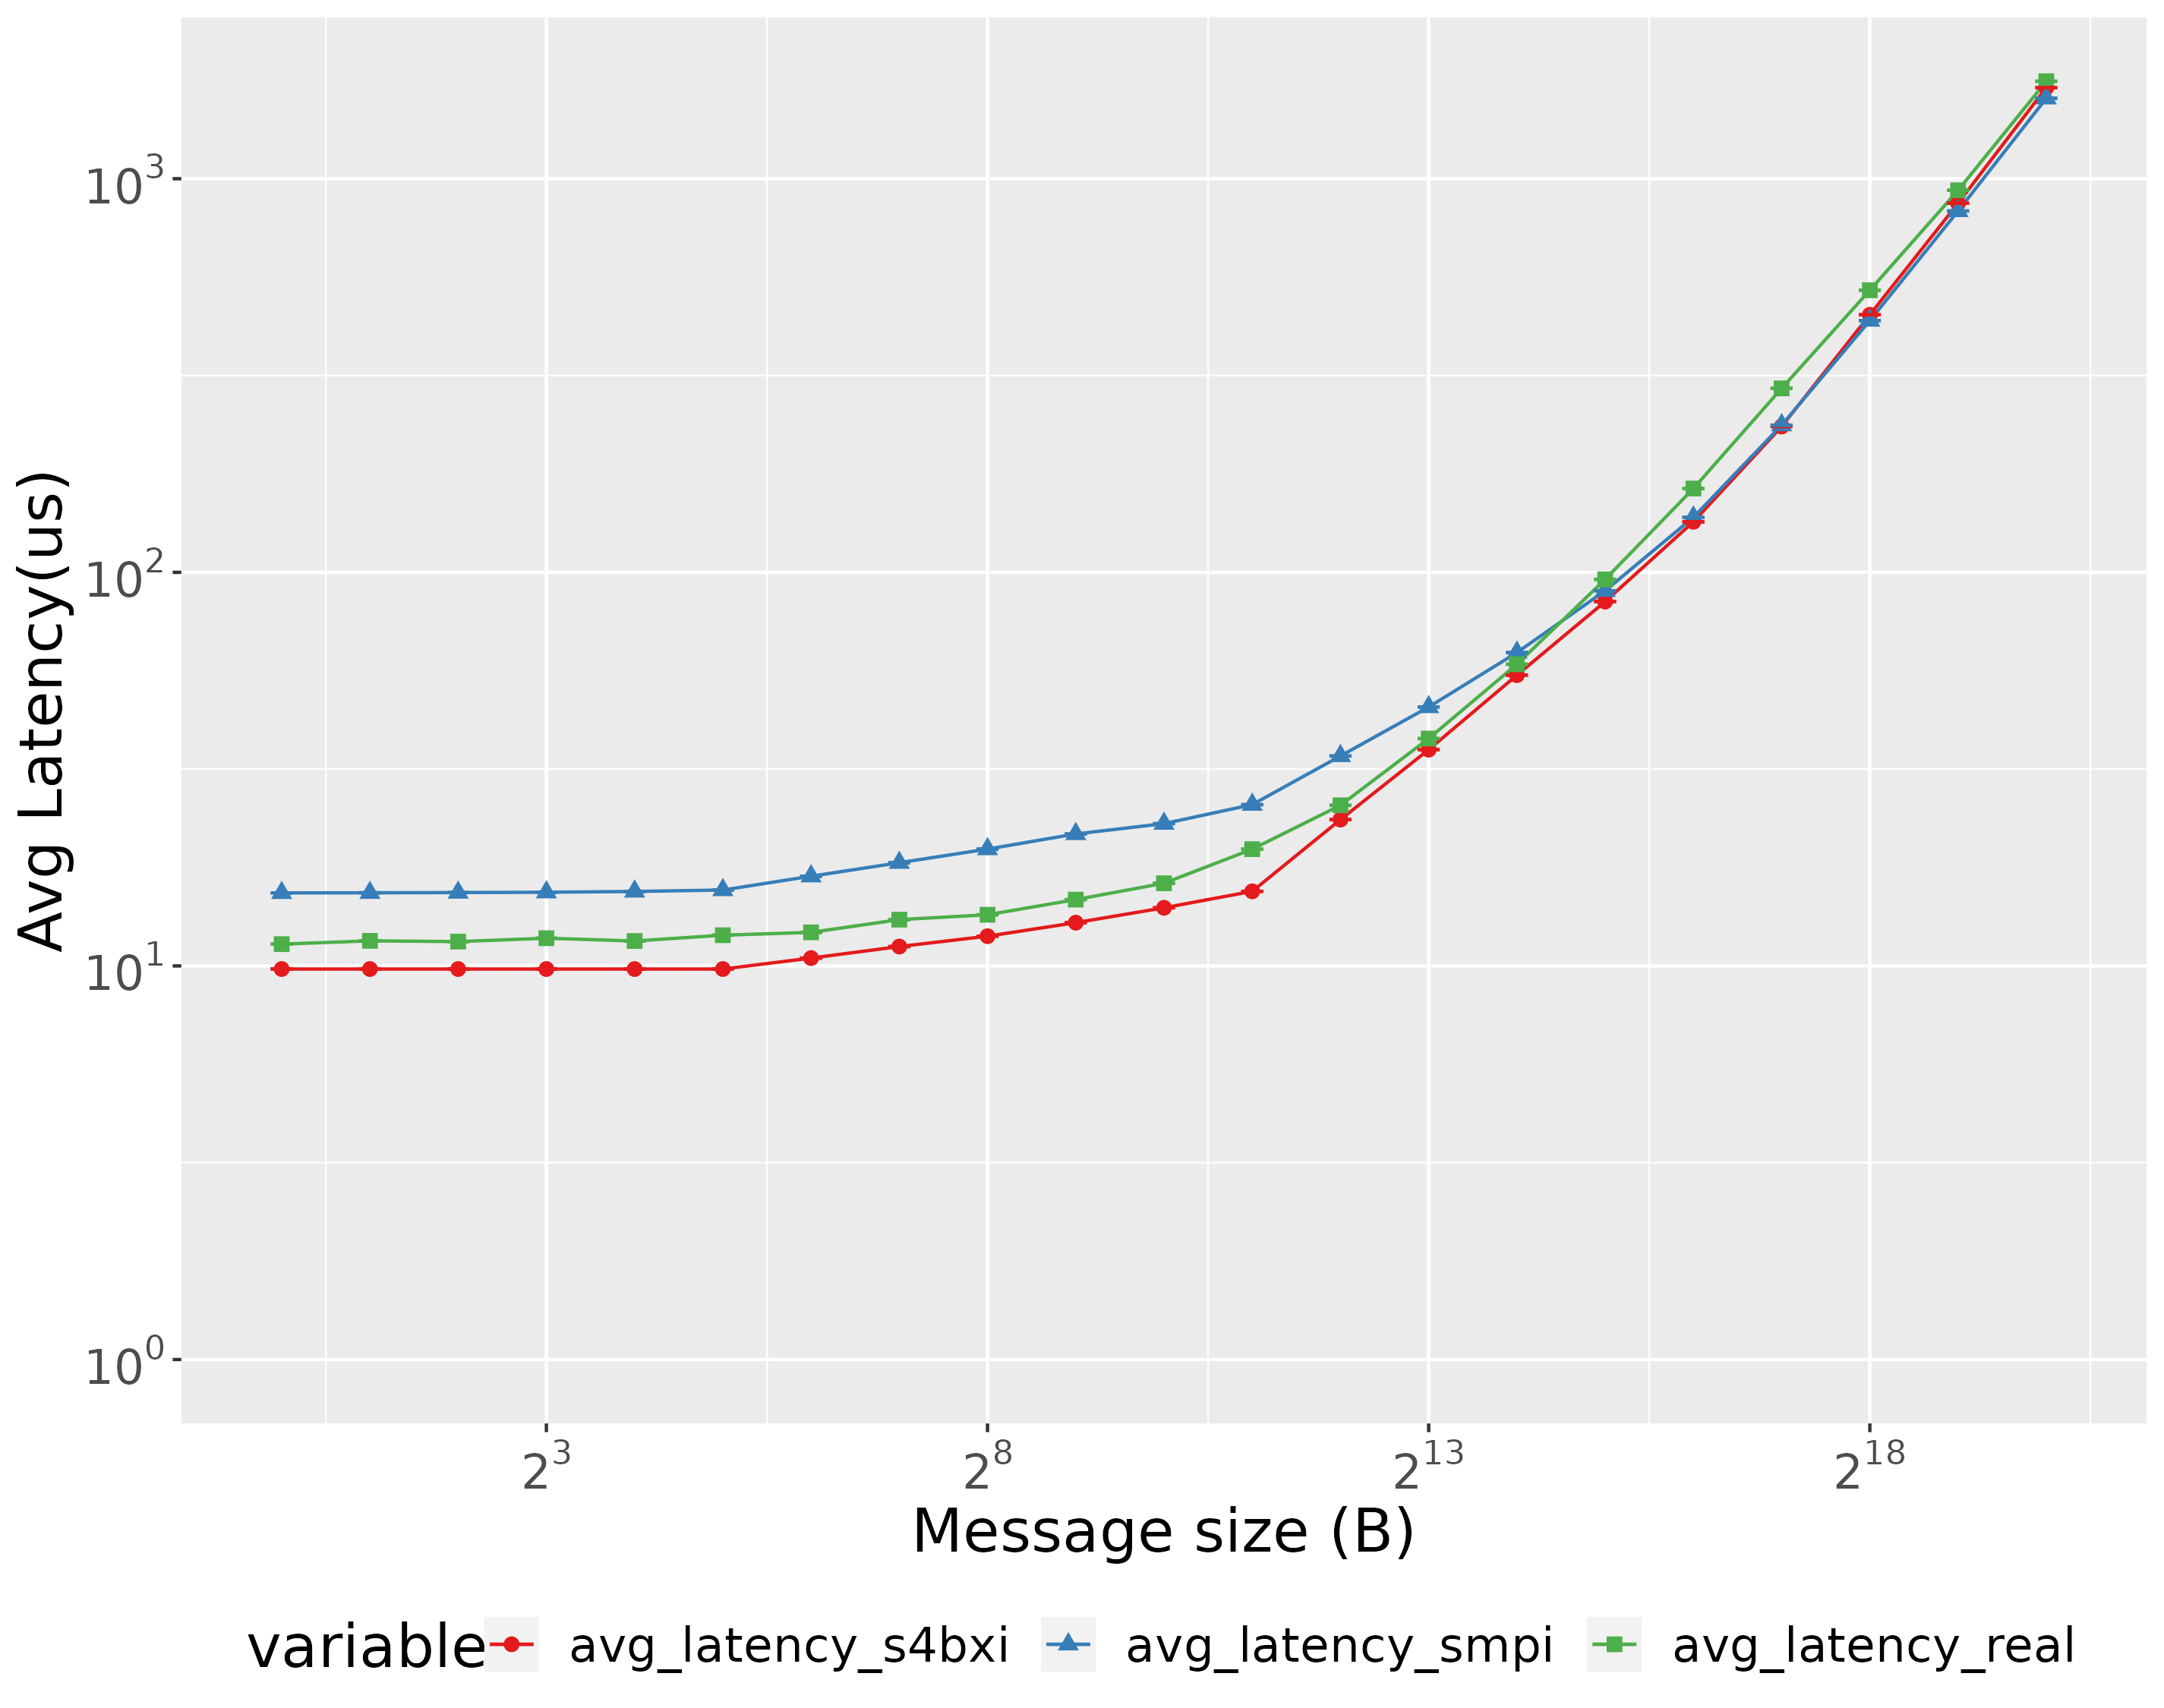
\includegraphics[width=0.88\textwidth]{5_high_level/OSU/allgather_16.png}
    \caption{OSU AllGather benchmark: comparison between the real-world run, an SMPI simulation, and an OpenMPI over S4BXI simulation}
    \label{fig:5_high_level:osu_allgather_16}
\end{figure}

\begin{figure}[!p]
    \centering
    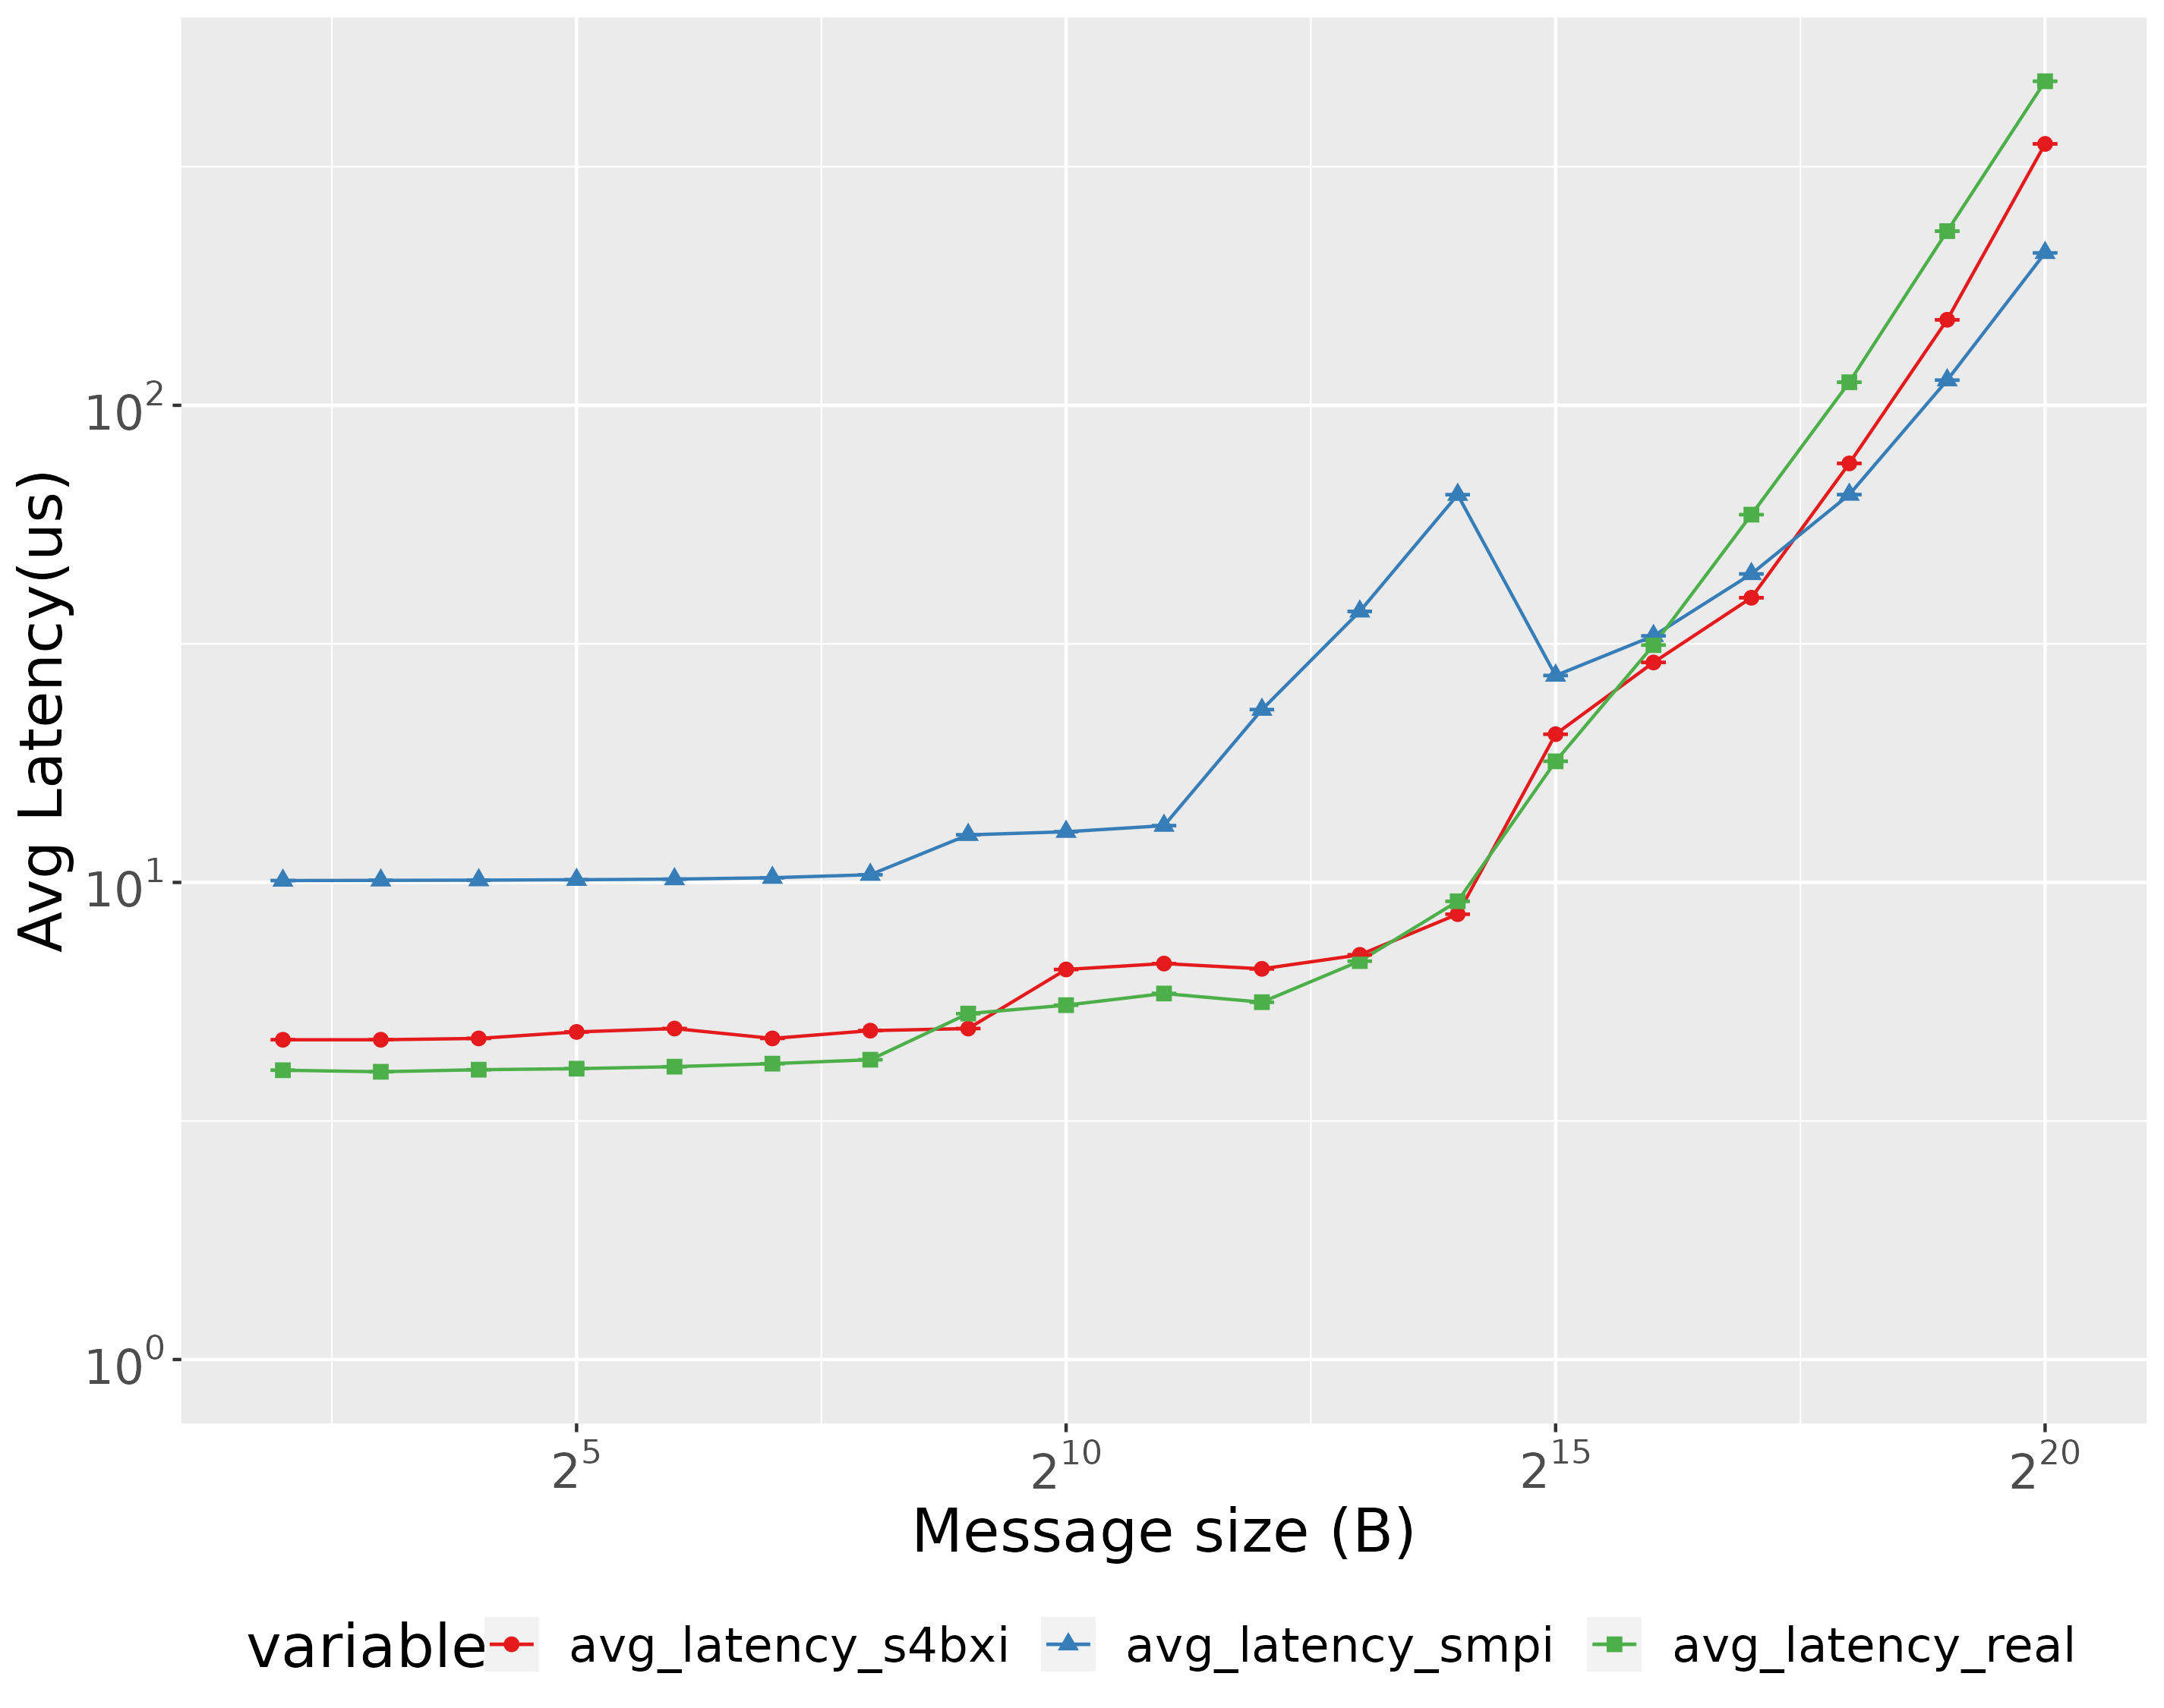
\includegraphics[width=0.88\textwidth]{5_high_level/OSU/reduce_16.png}
    \caption{OSU Reduce benchmark: comparison between the real-world run, an SMPI simulation, and an OpenMPI over S4BXI simulation}
    \label{fig:5_high_level:osu_reduce_16}
\end{figure}
\restoregeometry

In other cases, we can see a significant loss of accuracy for SMPI, usually for
specific message size. We can see an example of such a behaviour with the Reduce
benchmark, depicted on Figure~\ref{fig:5_high_level:osu_reduce_16}. Reduce
allows a ``root'' process to synthesize values from all processes into a single
value, by applying an arithmetic operation (for example a sum, taking the
maximum, etc.). In these cases, SMPI lacks accuracy because its implementation
of the collective operation does not match the algorithm used in Atos's version
of OpenMPI. Therefore, the sequence of point-to-point transfers that are
simulated is not an accurate model for the real-world benchmark, whereas in
S4BXI  we run the real-world MPI implementation  in our simulator. Consequently,
we get a realistic model of collective algorithms because of our simulation
method.

\begin{figure}[!ht]
    \centering
    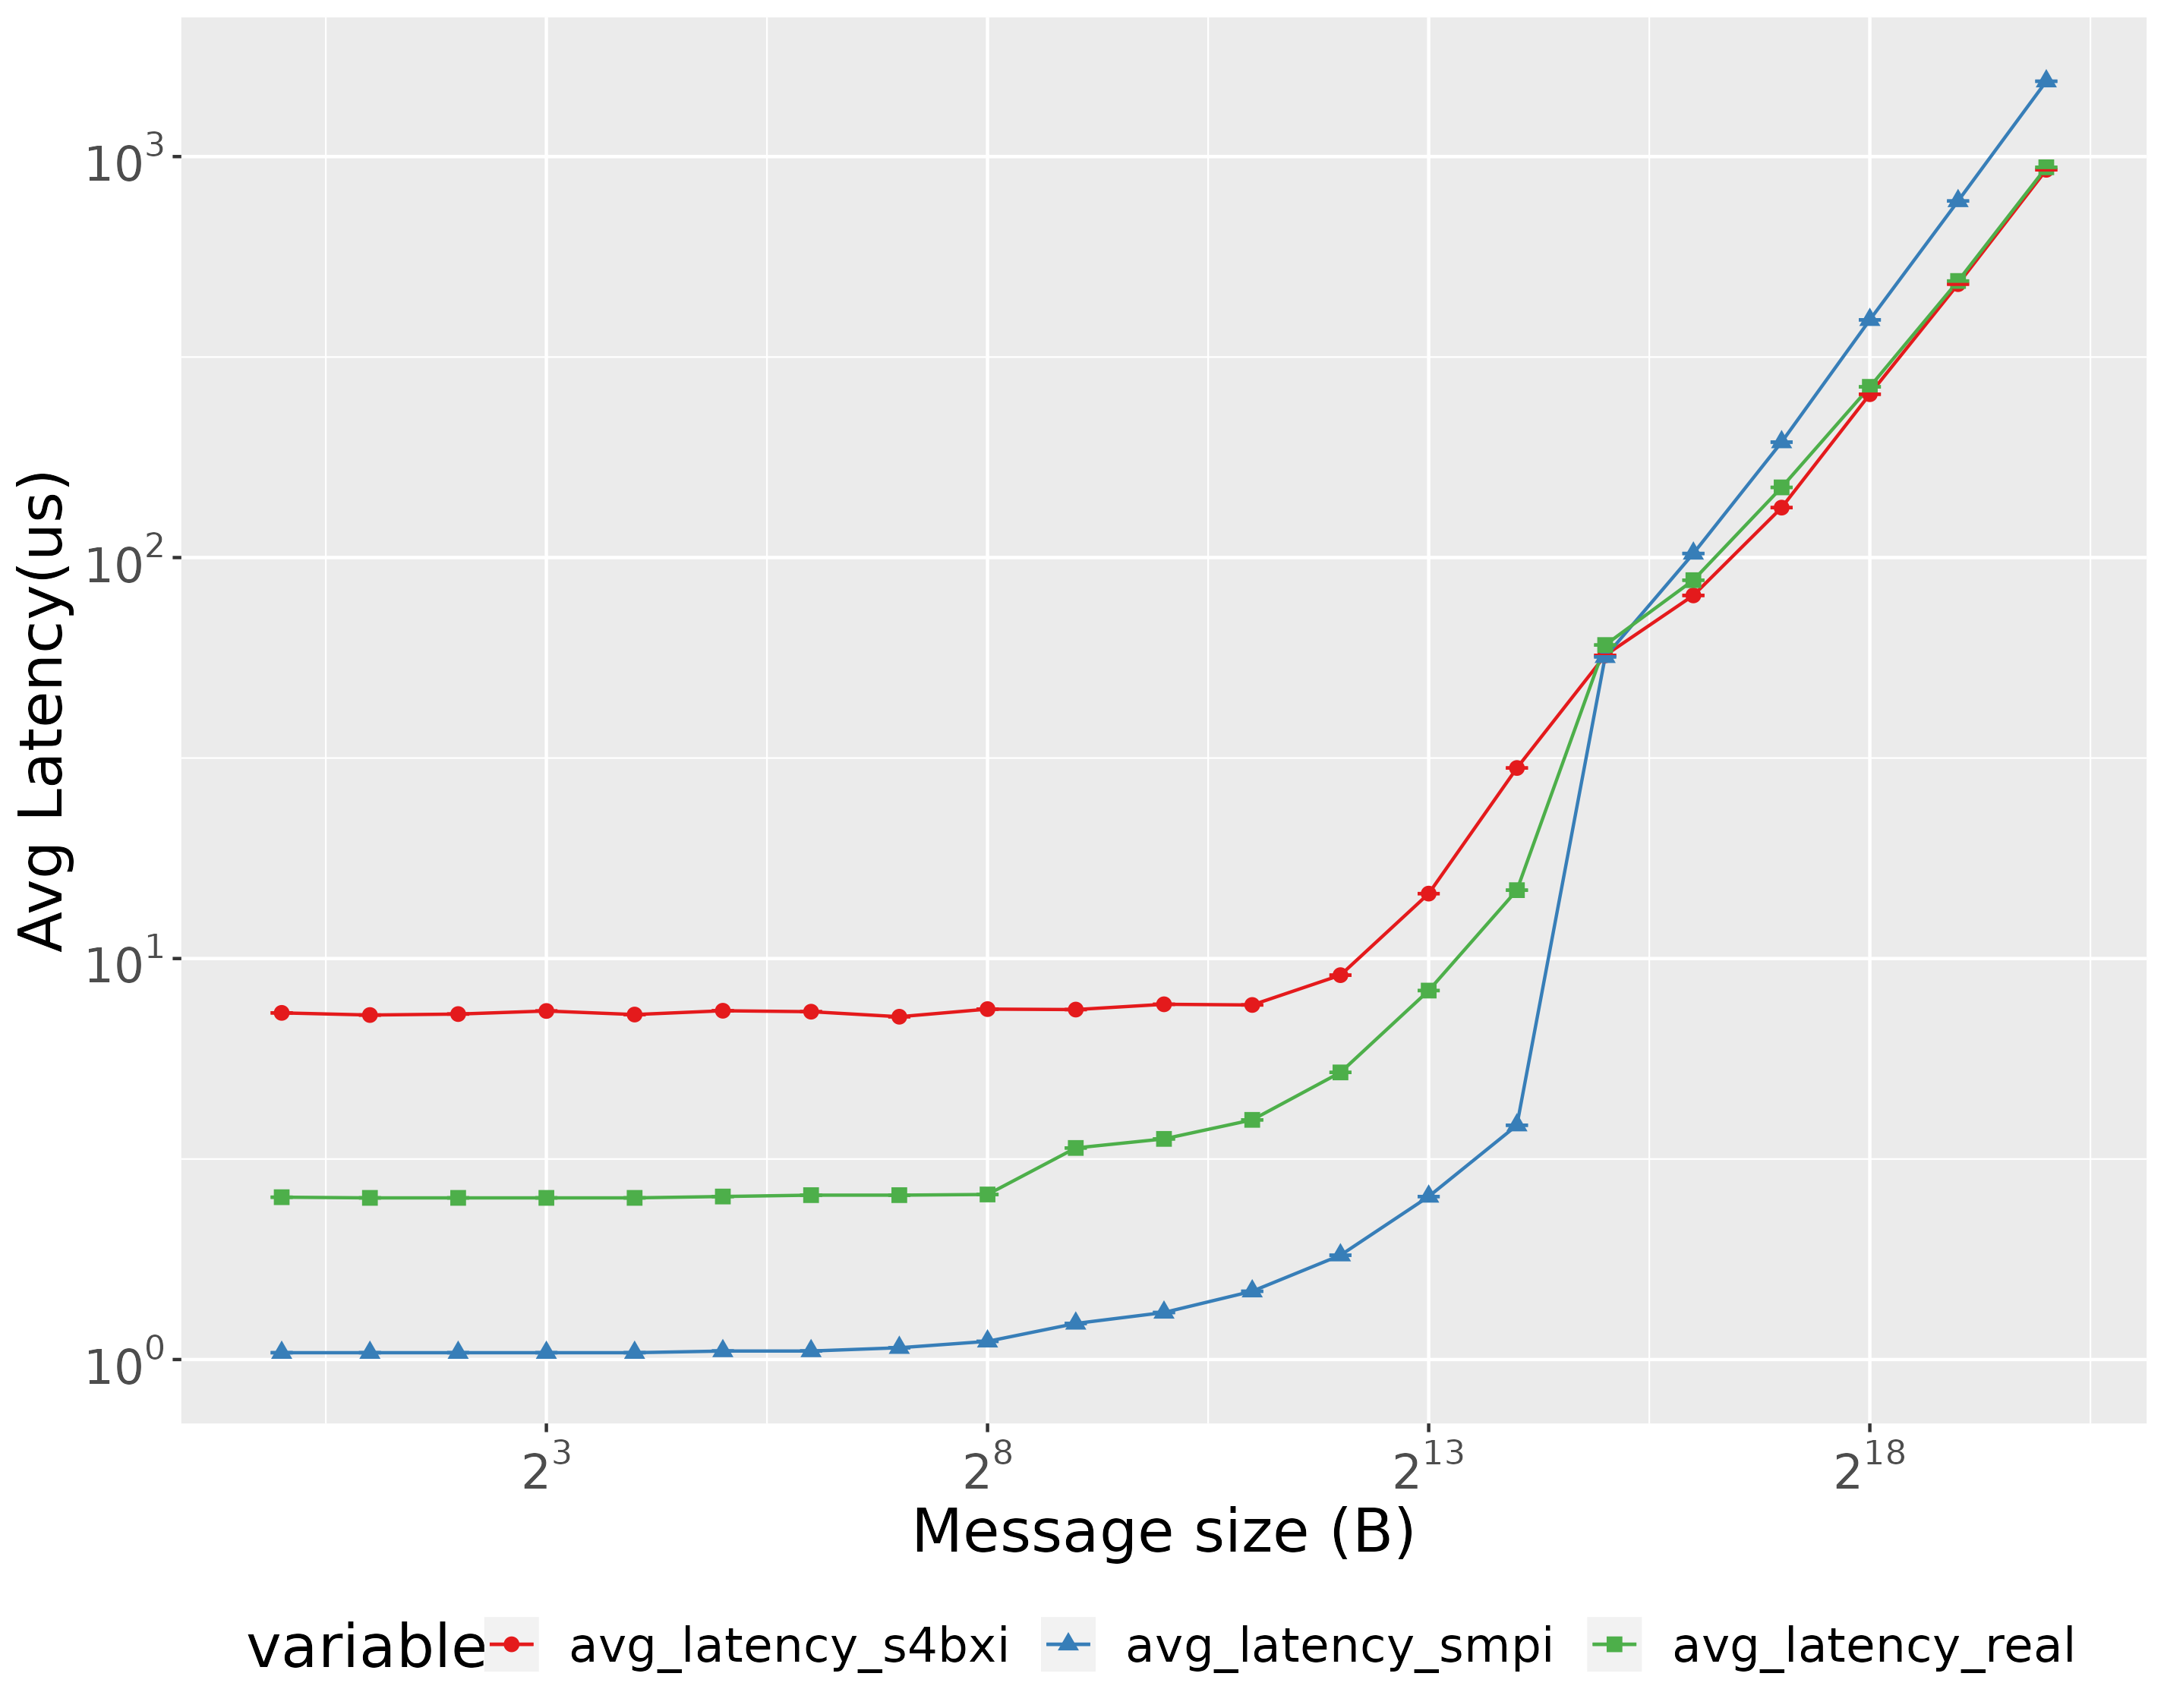
\includegraphics[width=0.88\textwidth]{5_high_level/OSU/gatherv_16.png}
    \caption{OSU GatherV benchmark: comparison between the real-world run, an SMPI simulation, and an OpenMPI over S4BXI simulation}
    \label{fig:5_high_level:osu_gatherv_16}
\end{figure}

Finally, there is one benchmark in particular that is particularly pathologic
for our simulation method: GatherV, which is depicted on
Figure~\ref{fig:5_high_level:osu_gatherv_16}. GatherV allows a ``root'' process
to fetch values from all processes, using non-continuous buffers. In this
experiment, OpenMPI over S4BXI is too pessimistic, while SMPI is too optimistic
but to a lesser degree. These results are very similar with the asynchronous
variant of this collective operation, IGatherV. These results are unusual
compared to the majority of our simulations, but we did not investigate them in
depth for two reasons. First, because of a lack of time, but also because we did
not encounter these operations in any of the applications that we executed in
simulation.

In order to get a more general view of our results compared to SMPI, we plotted
the average error of each simulation, by computing the absolute difference
between our simulation result and the value from the real-world experiment, and
averaging these values across all message sizes. The resulting graph is shown on
Figure~\ref{fig:5_high_level:osu_errors}.

We can see the three different patterns that we presented. First, most
simulations are of a similar accuracy in both approaches. In several other cases
simulations are significantly more precise in OpenMPI over S4BXI. Finally, there
are still a few operations for which both simulators have a high error, in some
of these cases our simulation method has an even larger error than SMPI, but
these cases are rare.

From a performance perspective, we can see on
Figure~\ref{fig:5_high_level:osu_perf} the slowdown of running a simulation
compared to performing an execution on a real-world cluster. Most of the time,
simulators are two orders of magnitude slower than real-world executions (around
100 times slower). This result is expected, as OSU benchmarks are extremely
communication-intensive, and therefore they stress our simulators to the
maximum. This figure also shows that S4BXI is generally slower than SMPI, which
comes from our architecture with more software layers, but the slowdown of our
approach is still of the same order of magnitude as state-of-the-art simulators.
In some rare cases, our approach even manages to be slightly faster, for
operations that are particularly costly to model in SMPI.

\begin{figure}[!hb]
    \centering
    \includegraphicsOverflow{5_high_level/OSU/OMPI_smpirun_16nodes1ppn_all.png}{1.2}
    \caption{Average error of both simulators: SMPI compared to OpenMPI over S4BXI}
    \label{fig:5_high_level:osu_errors}
\end{figure}

\begin{figure}[!hb]
    \centering
    \includegraphicsOverflow{5_high_level/OSU/OMPI_smpirun_16nodes1ppn_all_perf.png}{1.2}
    \caption{Average slowdown of both simulators compared to the real-world execution}
    \label{fig:5_high_level:osu_perf}
\end{figure}

\subsection{LULESH}

LULESH is a proxy application that is commonly used to assess the performance of
a cluster. In particular, it is frequently used to benchmark BXI, which is why
it is an interesting application to run in our model. As presented in
Section~\ref{subsubsec:2_context_hpc:LULESH}, LULESH has a few requirements: it
can only run on a number of MPI ranks that is the cube of an integer, for
example 1, 8, 27, 64, etc. processes. In our case, we are going to run this
application with 1 rank, 8 ranks on 8 machines (1 rank per machine), and 27
ranks on 9 machines (3 ranks per machine).

Each real-world experiment and each simulation is executed five times in order
to check the consistency of our results. LULESH is also executed for eleven
different problem sizes, which gives us executions that range from 0.15 seconds
up to a bit over a minute on the real-world cluster.

\begin{figure}[!ht]
    \centering
    \includegraphicsOverflow{5_high_level/LULESH/s4bxi_smpirun_no_vader_1ranks.png}{1.1}
    \caption{LULESH results on one MPI rank, comparing our simulator, SMPI, and a real-world execution (left graph shows accuracy, right graph shows performance)}
    \label{fig:5_high_level:s4bxi_smpirun_no_vader_1rank}
\end{figure}

Results are displayed for 1 MPI rank on
Figure~\ref{fig:5_high_level:s4bxi_smpirun_no_vader_1rank}, for 8 MPI ranks on
Figure~\ref{fig:5_high_level:s4bxi_smpirun_no_vader_8ranks}, and for 27 MPI
ranks on Figure~\ref{fig:5_high_level:s4bxi_smpirun_no_vader_27ranks}. The
simulation for only one process does not give us any information on the validity
of our network model, as there is no network communication, but it is a good
reference point to validate two things: first, that our model of computations
gives us accurate results, and second, that the performance of the simulators in
this scenario is good (that the overhead of running the application in
simulation is small). We can see on
Figure~\ref{fig:5_high_level:s4bxi_smpirun_no_vader_1rank} that these two
properties are indeed correct for both S4BXI and SMPI: on the left side, we can
see the time reported by LULESH at the end of its execution, which allows us to
assess the accuracy of the simulators. On the right side, we can see the
performance of the simulators compared to the execution time of the real-world
run. Both graphs show that the simulators are very close to the
real-world run.

\begin{figure}[!ht]
    \centering
    \includegraphicsOverflow{5_high_level/LULESH/s4bxi_smpirun_no_vader_8ranks.png}{1.1}
    \caption{LULESH results on 8 MPI ranks (8 nodes, 1 ranks per node), comparing our simulator, SMPI, and a real-world execution (left graph shows accuracy, right graph shows performance)}
    \label{fig:5_high_level:s4bxi_smpirun_no_vader_8ranks}
\end{figure}

On the other hand, on
Figure~\ref{fig:5_high_level:s4bxi_smpirun_no_vader_8ranks}, we can see the
result of an execution on 8 nodes (with 1 process per node), and the
corresponding simulations. We can see that the accuracy of both simulators is
still excellent, as they are very close to our reference values from the
real-world on all problem sizes. From a performance point of view, both
simulators are significantly slower than the real-world execution. This result
is expected, since all eight simulated processes are executed sequentially in
these single-threaded simulators (and therefore we expect a slowdown of at least
a factor of eight). We can also see that the S4BXI approach is slower than SMPI,
which once again is expected, since running a full OpenMPI implementation on top
of Portals is slower than running an MPI implementation that was specifically
optimized to run in SimGrid.

\begin{figure}[!ht]
    \centering
    \includegraphicsOverflow{5_high_level/LULESH/s4bxi_smpirun_no_vader_27ranks.png}{1.1}
    \caption{LULESH results on 27 MPI ranks (9 nodes, 3 ranks per node), comparing our simulator, SMPI, and a real-world execution. Vader is disabled in real-world OpenMPI and OpenMPI over S4BXI}
    \label{fig:5_high_level:s4bxi_smpirun_no_vader_27ranks}
\end{figure}

Finally, the execution on 27 ranks (with 9 nodes and 3 processes per node)
allows us to test further the network model of each simulator, and also to make
sure that intra-node communications give accurate results. As presented in
Section~\ref{sec:5_high_level:shared_mem_support}, intra-node communications can
be performed in two different ways: either using the Vader BTL, or simply by
going through Portals. Of course, enabling Vader to perform communications
across shared memory is irrelevant in SMPI, as it does not feature such
low-level configuration options. The results are displayed on
Figure~\ref{fig:5_high_level:s4bxi_smpirun_no_vader_27ranks} with Vader disabled
on the real-world execution and OpenMPI over S4BXI, and on
Figure~\ref{fig:5_high_level:s4bxi_smpirun_vader_emulated_27ranks} with Vader
enabled. We can see that the results are very similar in both cases, and that
our two simulators perform well regardless of whether we use Vader or not. The
reason why the performance of LULESH is identical whether we use Vader or not,
comes from the efficiency of BXI NICs. Indeed, when Portals is used to transfer
data between two processes on the same machine, the NIC effectively acts as a
DMA controller, which copy the payload from the source buffer of the sender
process to the reception buffer of the target process. This is very similar to
how Vader operates, using shared memory to copy data between processes,
therefore it is expected to observe a similar performance. Once again, we see a
considerable loss of performance compared to the execution on 8 processes, which
corresponds to what we expected (as we now run 27 MPI ranks in a single thread
in our simulators).

\begin{figure}[!ht]
    \centering
    \includegraphicsOverflow{5_high_level/LULESH/s4bxi_smpirun_vader_emulated_27ranks.png}{1.1}
    \caption{LULESH results on 27 MPI ranks (9 nodes, 3 ranks per node), comparing our simulator, SMPI, and a real-world execution. Vader enabled in real-world OpenMPI and OpenMPI over S4BXI}
    \label{fig:5_high_level:s4bxi_smpirun_vader_emulated_27ranks}
\end{figure}

The conclusion of this experiment is that while both simulators have a very good
accuracy when running LULESH, our approach does not offer any benefit over SMPI,
as the accuracy is similar, and the performance inferior. This result is not
very surprising, as LULESH relies heavily on point-to-point communication (with
little collective operations). Since SMPI is calibrated specifically on these
point-to-point primitives, it is expected to get very good results, and these
experiments validate that our calibration of the network parameters of SMPI is
accurate too.

\subsection{Quicksilver}
\label{subsec:5_high_level:quicksilver}

Quicksilver is an application that performs ten independent cycles of
computations on a configurable number of particles. At the end of the execution,
Quicksilver reports three performance values for each cycle of computations: the
time taken by the initialization, the ``tracking'' phase (where most
computations happen), and the finalization of the cycle. In practice, we have
observed that the initialization and finalization phase of each cycle have a
duration which is negligible compared to the ``tracking'' phase, therefore we
will only show the tracking times of each cycle in our graphs, for more clarity.
We have run Quicksilver for different particle numbers, ranging from 10,000 up
to 1,000,000, and many cluster configurations: we used platforms with all
combinations of 1, 2, 4, 8 and 16 nodes with 1, 2 and 4 processes per node.
Since the resulting graphs are very numerous, in this section we will present a
few representative cases of the types of results we obtained.

From a technical point of view, the simulations were performed on one of the
machines from the real-world cluster, with an AMD EPYC™ 7763 64-Core processor.
Every real-world execution was executed five times, and each simulation was
executed twice (because of a lack of time towards the end of this thesis).
Additionally, once again we had the choice of enabling Vader or not when using
several processes per node. We observed little difference with and without Vader
in our results (both in simulation and the real world experiments), therefore we
will only present experiments performed without Vader, in order to reduce the
number of variables to analyze in this section.

\begin{figure}[!b]
    \centering
    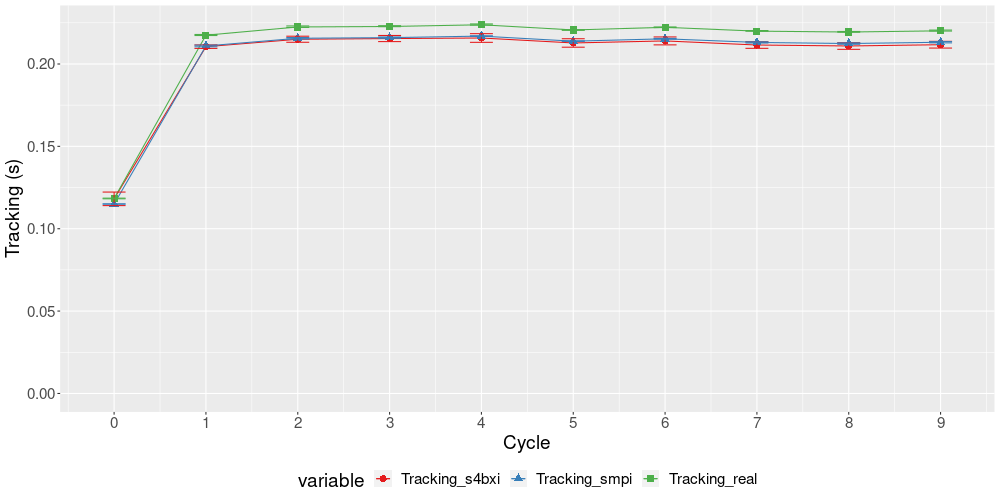
\includegraphics[width=1\textwidth]{5_high_level/Quicksilver/10000particles_1tasks_1ppn.png}
    \caption{Quiksilver experiment on 10,000 particles, with 1 node and 1 process per node}
    \label{fig:5_high_level:quicksilver_1tasks_1ppn}
\end{figure}

We will start by analyzing small problem sizes, with only 10,000 particles.
First, as with LULESH, we can see that both simulators give a very good result
when running Quicksilver on only one node with only one process, which is
depicted on Figure~\ref{fig:5_high_level:quicksilver_1tasks_1ppn}. This is
expected of course, since the simulators are running the application with no
communications, but it allows us to confirm that both simulators work and that
we get the same output in simulation and the real-world experiment.

\begin{figure}[!tb]
    \centering
    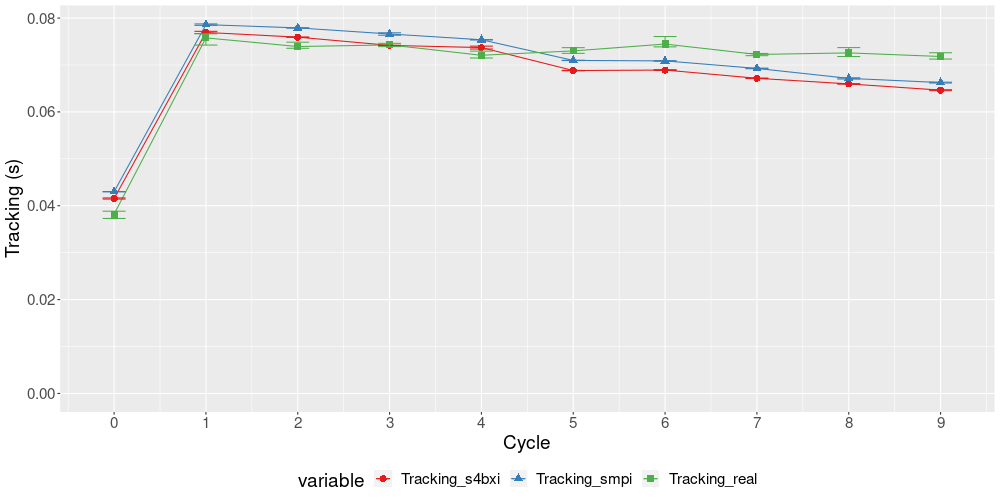
\includegraphics[width=1\textwidth]{5_high_level/Quicksilver/10000particles_4tasks_1ppn.png}
    \caption{Quiksilver experiment on 10,000 particles, with 4 nodes and 1 process per node}
    \label{fig:5_high_level:quicksilver_4tasks_1ppn}
\end{figure}


With very small cluster sizes, we can see that both simulators continue to have
a good accuracy. For example,
Figure~\ref{fig:5_high_level:quicksilver_4tasks_1ppn} shows the result of
executing Quicksilver on four nodes, with one process per node, and still 10,000
input particles.


\begin{figure}[!tb]
    \centering
    \includegraphics[width=1\textwidth]{5_high_level/Quicksilver/10000particles_8tasks_1ppn.png}
    \caption{Quiksilver experiment on 10,000 particles, with 8 nodes and 1 process per node}
    \label{fig:5_high_level:quicksilver_8tasks_1ppn}
\end{figure}

On the other hand, as soon as we use more than 8 MPI ranks (regardless of the
number of nodes), we observe a quick degradation of the accuracy of SMPI, while
OpenMPI over S4BXI keeps a good accuracy. We can see the start of this trend
with an execution on eight nodes and one process per node on
Figure~\ref{fig:5_high_level:quicksilver_8tasks_1ppn}. It only gets worse for
larger numbers of MPI ranks, as we can see on
Figure~\ref{fig:5_high_level:quicksilver_16tasks_1ppn} for 16 nodes and one
process per node, or Figure~\ref{fig:5_high_level:quicksilver_16tasks_4ppn} for
four nodes and four processes per node (so 16 processes in total again).


\begin{figure}[!tb]
    \centering
    \includegraphics[width=1\textwidth]{5_high_level/Quicksilver/10000particles_16tasks_1ppn.png}
    \caption{Quiksilver experiment on 10,000 particles, with 16 nodes and 1 process per node}
    \label{fig:5_high_level:quicksilver_16tasks_1ppn}
\end{figure}

\begin{figure}[!tb]
    \centering
    \includegraphics[width=1\textwidth]{5_high_level/Quicksilver/10000particles_16tasks_4ppn.png}
    \caption{Quiksilver experiment on 10,000 particles, with 4 nodes and 4 processes per node}
    \label{fig:5_high_level:quicksilver_16tasks_4ppn}
\end{figure}

As we increase the number of particles given as an input to Quicksilver, we can
observe the same phenomenon. The only difference is that as we increase the
problem size, SMPI remains accurate for larger cluster sizes, but we always
observe a point where SMPI's accuracy drops dramatically. For example, with
1,000,000 particles, we conserve a good accuracy of both simulators up to 16 MPI
ranks, as we can see on Figure~\ref{fig:5_high_level:quicksilver_16tasks_2ppn}
(with eight nodes and two process per node). Starting from 32 MPI ranks, we can
see the accuracy of SMPI drops, for example on
Figure~\ref{fig:5_high_level:quicksilver_32tasks_2ppn}.

\begin{figure}[!tb]
    \centering
    \includegraphics[width=1\textwidth]{5_high_level/Quicksilver/1000000particles_16tasks_2ppn.png}
    \caption{Quiksilver experiment on 1,000,000 particles, with 8 nodes and 2 processes per node}
    \label{fig:5_high_level:quicksilver_16tasks_2ppn}
\end{figure}

\begin{figure}[!tb]
    \centering
    \includegraphics[width=1\textwidth]{5_high_level/Quicksilver/1000000particles_32tasks_2ppn.png}
    \caption{Quiksilver experiment on 1,000,000 particles, with 16 nodes and 2 processes per node}
    \label{fig:5_high_level:quicksilver_32tasks_2ppn}
\end{figure}

This lack of accuracy from SMPI is highly unexpected, as we never obtained
results so far away from the real-world experiment in OSU benchmarks or LULESH.
We were not able to identify what could be so detrimental to the SMPI model in
Quicksilver, only that the accuracy drop is very consistent, and depends on the
problem size and the number of MPI ranks, regardless of the number of nodes they
are distributed on.

\subsection{High-Performance Linpack (HPL)}

Finally, we tested our simulator on HPL. This application is particularly
interesting to study because we can use two different versions: in addition to
the ``regular'' version of HPL, we can use a skeleton version of the
application, made by Tom \textsc{Cornebize} during his PhD~\cite{Cornebize2021}.
The idea behind this version of HPL is that it performs the same communications
as the full application, but it replaces the most costly computation phases with
a delay that estimates the corresponding CPU time and which is simulated
instantaneously. The skeleton version does not compute the same result as the
original application but its simulated execution time is approximately the same.
In practice, the vast majority of the CPU time of the benchmark is spent in one
function (\inline{HPL_dgemm}), which performs a Double precision GEneral Matrix
Multiply (DGEMM). Therefore, we can save a lot of time in simulation be removing
the code of this function, and by replacing it with a function call to our
simulator in order to inject an artificial amount of computation time in the
model directly. Of course, this skeleton version of HPL does not perform
accurate computations, as many CPU operations were removed, but the timing of
HPL in simulated time is preserved because the operations that we removed do not
affect the execution flow of HPL.

\begin{figure}[!ht]
    \centering
    \includegraphicsOverflow{5_high_level/HPL/vanilla/__2nodes_1ppn_chap_5.png}{1.1}
    \caption{HPL experiment on 2 nodes with 1 process per node}
    \label{fig:5_high_level:hpl_vanilla_2x1}
\end{figure}

We will start by presenting our results for the full version of the application:
Figure~\ref{fig:5_high_level:hpl_vanilla_2x1} shows data from both simulators
(SMPI and OpenMPI over S4BXI) compared to real-world executions, for a very
small number of MPI ranks: two nodes with only one process per node. The left
graph shows the precision of the simulators, by plotting the performance
reported by HPL (in GFlops), whereas the right graph plots the performance of
the simulators (with respect to wall-clock time), compared to the duration of
the real-world experiment. We can see that even though the real-world
experiments show a surprising evolution of the computing power (in Gflops) when
the problem size increases, both simulators manage to model these effects
accurately. As the number of processes is very small, we can see that the
performance of both simulators is reasonably good, and that for large problem
sizes they perform very similarly.

\begin{figure}[!ht]
    \centering
    \includegraphicsOverflow{5_high_level/HPL/vanilla/__10nodes_5ppn_chap_5.png}{1.1}
    \caption{HPL experiment on 50 MPI ranks (10 nodes with 5 processes per node)}
    \label{fig:5_high_level:hpl_vanilla_10x5}
\end{figure}

\begin{figure}[!ht]
    \centering
    \includegraphicsOverflow{5_high_level/HPL/vanilla/__16nodes_8ppn_chap_5.png}{1.1}
    \caption{HPL experiment on 128 MPI ranks (16 nodes with 8 processes per node)}
    \label{fig:5_high_level:hpl_vanilla_16x8}
\end{figure}


\begin{figure}[!th]
    \centering
    \includegraphicsOverflow{5_high_level/HPL/optimized_grid5000_tuning/__2nodes_1ppn_chap_5.png}{1.1}
    \caption{HPL skeleton experiment on 2 nodes with 1 process per node}
    \label{fig:5_high_level:hpl_optimized_2x1_grid5000}
\end{figure}

\begin{figure}[!th]
    \centering
    \includegraphicsOverflow{5_high_level/HPL/optimized_grid5000_tuning/__10nodes_5ppn_chap_5.png}{1.1}
    \caption{HPL skeleton experiment on 50 MPI ranks (10 nodes with 5 processes per node)}
    \label{fig:5_high_level:hpl_optimized_10x5_grid5000}
\end{figure}

Executions with more MPI ranks are displayed on
Figure~\ref{fig:5_high_level:hpl_vanilla_10x5} for 50 MPI ranks (ten nodes and
five processes per node) and on Figure~\ref{fig:5_high_level:hpl_vanilla_16x8}
for 128 MPI ranks (16 nodes and eight processes per node). On both figures we
can see that the accuracy of the simulators is comparable, with a slight
advantage for SMPI. This result is not surprising, because of how HPL uses MPI:
even though the benchmark needs to be able to perform collective communications,
it does not use the collective primitives offered by MPI. Instead, all
operations are re-implemented in HPL with a combination of basic ``send'' and
``receive'' point-to-point primitives. Since SMPI's network model is
specifically tuned to perform well on these point-to-point operations (using
coefficients on the latency and bandwidth of Links), it is expected to get good
results in this context. In comparison, OpenMPI over S4BXI models low-level
network operations, which also gives good results. Nevertheless, in order to
surpass the accuracy of SMPI on this type of workload, our approach would
require a finer tuning of very low-level parameters inside our simulator. From a
performance perspective, as expected the duration of simulation increases with
the number of simulated MPI ranks. We can see that the gap between the
performance of SMPI and OpenMPI over S4BXI increases when we simulate more MPI
ranks, as we can see in Figure~\ref{fig:5_high_level:hpl_vanilla_2x1} where both
simulators are extremely close, whereas the gap is a lot more important on
figures~\ref{fig:5_high_level:hpl_vanilla_10x5}
and~\ref{fig:5_high_level:hpl_vanilla_16x8}. This different in scaling is
expected, since the proportion of network operations (compared to the
computational phases) increases as well, and modelling communications is more
costly with our approach than SMPI (which has a more simplistic network model).

\begin{figure}[!th]
    \centering
    \includegraphics[width = 1\textwidth]{5_high_level/HPL/tuning/MNK.png}
    \caption{Duration of \inline{HPL_dgemm} as a function of $M \times N \times K$}
    \label{fig:5_high_level:hpl_optimized_MNK}
\end{figure}

\begin{figure}[!th]
    \centering
    \includegraphicsOverflow{5_high_level/HPL/4x4_no_vader_144_optimized_tuned.png}{1.1}
    \caption{HPL skeleton experiment on 16 MPI ranks (4 nodes with 4 processes per node), with our tuning}
    \label{fig:5_high_level:hpl_optimized_4x4}
\end{figure}

In order to improve the performance of the simulators, we can use the skeleton
version at our disposal. However, the main difficulty is to tune the artificial
computation time to inject in SimGrid (in the \inline{HPL_dgemm} function). In
his PhD, Tom \textsc{Cornebize} uses machines from the Grid5000 testbed, and we
re-used his tuning without any modifications at first. Results are depicted on
Figure~\ref{fig:5_high_level:hpl_optimized_2x1_grid5000} for two MPI ranks (two
nodes and one process per node) and on
Figure~\ref{fig:5_high_level:hpl_optimized_10x5_grid5000} for 50 MPI ranks (ten
nodes and five processes per node). From a performance perspective, we can see
that both simulators are sped up significantly (the SMPI simulation on two MPI
ranks is even faster than the real world experiment for all problem sizes). Of
course, the gap between the execution time of the simulators stays significant,
as the network model of our approach is still costly on the skeleton version (as
the number of communications is identical). Regarding accuracy, we can see that
this version of HPL (with this tuning) made both simulators very pessimistic,
which shows that the CPUs on our clusters are much more efficient at running
DGEMM operations than Grid5000's ones.


\begin{figure}[!ht]
    \centering
    \includegraphicsOverflow{5_high_level/HPL/4x4_no_vader_144_vanilla.png}{1.1}
    \caption{Full HPL experiment on 16 MPI ranks (4 nodes with 4 processes per node)}
    \label{fig:5_high_level:hpl_vanilla_4x4}
\end{figure}

To get a better tuning of our DGEMM model, we instrumented the real-world
version of HPL to measure the duration of the \inline{HPL_dgemm} primitive as a
function of its numerical parameters (which are called $M$, $N$ and $K$). By
plotting the performance of \inline{HPL_dgemm} as a function of each combination
of the parameters ($M$, $N$, $K$, $M \times N$, $M \times K$, $N \times K$ and
$M \times N \times K$), we identified that the execution time of
\inline{HPL_dgemm} seems close to a linear function of $M \times N \times K$
(with a significant amount of noise):
Figure~\ref{fig:5_high_level:hpl_optimized_MNK} shows this data, depicted along
with the corresponding linear regression. Consequently, we managed to tune the
estimation of the computation time; this allowed us to get the results depicted
on Figure~\ref{fig:5_high_level:hpl_optimized_4x4}. The corresponding run of the
full benchmark (on 16 MPI ranks) is shown on
Figure~\ref{fig:5_high_level:hpl_vanilla_4x4}. As we can see, even if our
heuristic to estimate the duration of \inline{HPL_dgemm} is better adapted to
our cluster, it is still far from perfect. This is expected since our tuning is
more simplistic than the study conducted by Tom \textsc{Cornebize}.

The most important takeaway from these experiments is that this type of skeleton
application, originally designed for SMPI, is fully compatible with S4BXI
simulations out of the box. Even though the improvement in performance is not as
important with our model as it is with SMPI, we showed that this type of patch
to an application works in an identical way in S4BXI and SMPI, as we can see
from the accuracy graphs.

\section{OpenSHMEM}

While modeling MPI is the main usage of our simulator, one of the strengths of
S4BXI is its adaptability: since it is modeling a low-level API, it can be used
to run a variety of higher-level APIs. To demonstrate that, we have worked on
the simulation of the OpenSHMEM library.

\subsection{Running OpenSHMEM in S4BXI}

OpenSHMEM follows a Partitioned global address space (PGAS) model, which means
that, compared to MPI, it focuses less on message passing. Instead, it gives
every process in the job a transparent view of a ``global memory pool'', which
in practice is distributed across several nodes. For our study we adapted Atos's
version of OpenSHMEM to support running on S4BXI. The Atos version is very
similar to Sandia's implementation of OpenSHMEM
(\url{https://github.com/Sandia-OpenSHMEM/SOS}), with only minor modifications
to support execution over BXI.

Similarly to OpenMPI, we chose to add support for OpenSHMEM simulation over
S4BXI by adding a small patch to OpenSHMEM. The architecture of OpenSHMEM's code
proved to be easier to work with for our purpose, because the project's scale is
significantly smaller, therefore making a preliminary patch to run this library
in simulation was much easier than the same developments in OpenMPI. In the end,
our patch simply adds a new file to OpenSHMEM, and the only modifications we
made to existing code was in the build scripts to include our new file.
Internally, OpenSHMEM uses a concept of a ``runtime'' that should be
initialized. The project natively provides four runtimes: one over MPI, and
three over various versions of PMI (PMI, PMI2 and PMIx). Therefore,  to add
support for S4BXI we only need a new runtime, which implements basic utilities
(like a barrier, basic metadata exchange), and we are ready to perform
simulations. This runtime only consists of 11 functions, most of which are
trivially implemented using S4BXI: the vast majority are implemented in one line
of code, and the largest one only has five lines of code. The full runtime is
given in Appendix~\ref{app:oshmem_code}.

Because of time constraints, and because our main goal was simulating MPI
accurately, we did not study OpenSHMEM benchmarks with as much detail as MPI
ones. The validation we performed focused on two aspects: the unit test suite
provided with OpenSHMEM, and the OSU-microbenchmarks (which also have an
OpenSHMEM variant even though the MPI benchmarks are more notorious).

\subsection{Experimental validation}

\begin{figure}[!b]
    \centering
    \includegraphics[width = 0.8\textwidth]{5_high_level/OpenSHMEM/put_2.png}
    \caption{Benchmark of the ``put'' operation of OpenSHMEM between 2 nodes}
    \label{fig:5_high_level:shmem_put}
\end{figure}

In order to test our simulations of OpenSHMEM, we first ran the unit test suite
provided by OpenSHMEM in our simulator, on a desktop computer. Every test was
executed four times: with 2, 4, 8 and 16 nodes and always one process per node,
this amounts to 392 runs in total. We used a fairly low value for the timeout,
of one minute, because we observed that most successful tests ran in a few
seconds only. The results are mixed: while the majority of tests pass -- 228
executions succeed -- we still have 154 errors, and 10 timeouts. Indeed, we
expected some tests to fail, as they perform operations that are not supported
by our simulators, such as using \inline{pthread} mutexes which are not properly
intercepted by S4BXI. However, the amount of errors is still a lot more
important than what we expected, and too large  to reliably run OpenSHMEM in
simulation. Nevertheless, these results show that with few efforts we are
already close to having a functional OpenSHMEM simulator, as most basic tests
work as expected.

\begin{figure}[!h]
    \centering
    \includegraphics[width = 0.8\textwidth]{5_high_level/OpenSHMEM/get_2.png}
    \caption{Benchmark of the ``get'' operation of OpenSHMEM between 2 nodes}
    \label{fig:5_high_level:shmem_get}
\end{figure}

Running OpenSHMEM was only a side experiment in this thesis, and we did not
invest the time required to fully debug the problems. The only hypothesis that
we have is that OpenSHMEM tries to locate memory regions inside the current
binary at startup, which might cause problems in simulation since we do not
execute applications directly from their binary, but instead we run them from a
shared library which is opened by our entry point, \inline{s4bximain}. In the
real-world, each process would be isolated by the operating system and deployed
on several machines, but in simulation OpenSHMEM might locate the same memory
region for all processes (by looking directly in \inline{s4bximain}) with no
isolation. This could cause issues but would require further investigations.

After running unit tests, we tried the OpenSHMEM variant of OSU benchmarks. Once
again, some tests do not terminate properly, therefore we only present a few of
those which work correctly, in order to give an idea of the precision that we
can expect out of OpenSHMEM simulation. For point to point operations, we can
see on Figure~\ref{fig:5_high_level:shmem_put} the result of the ``put''
benchmark between two nodes (which correspond to a remote write), and on
Figure~\ref{fig:5_high_level:shmem_get} we have a similar benchmark for the
``get'' operation (remote read). We can see that the accuracy is not perfect,
especially for ``put'' operations of a small size, but overall it is already
acceptable, even though we did not perform any particular tuning to make
OpenSHMEM simulations more accurate.

\begin{figure}[!hb]
    \centering
    \includegraphics[width = 0.8\textwidth]{5_high_level/OpenSHMEM/fcollect_8.png}
    \caption{Benchmark of the ``fcollect'' operation of OpenSHMEM using 8 nodes}
    \label{fig:5_high_level:shmem_fcollect}
\end{figure}

\begin{figure}[!hb]
    \centering
    \includegraphics[width = 0.8\textwidth]{5_high_level/OpenSHMEM/reduce_16.png}
    \caption{``Reduce'' OSU benchmark using 16 nodes}
    \label{fig:5_high_level:shmem_reduce}
\end{figure}

For collective operations, we can see on
Figure~\ref{fig:5_high_level:shmem_fcollect} the result of the ``fcollect''
benchmark on eight nodes, which concatenates data from multiple processes into a
buffer on every process of the job. Finally,
Figure~\ref{fig:5_high_level:shmem_reduce} shows the result of the ``reduce''
benchmark on 16 nodes, which performs various reduction operations (min, max and
sum) using data from all processes (similarly to MPI's reduce operation). We can
see that the conclusion is the same on collective operation than with
point-to-point ones: overall the accuracy is acceptable, even though in this
case we can see some unexpected performance jumps, that we did not investigate
because of a lack of time.

\section{Summary}

Simulating high-level APIs with our method has proved perfectly achievable, even
if some development time has been required. Even though our simulations are
slower than real-world experiments, they have other advantages: they only use
one CPU core, therefore exploring a vast parameter space can be done in parallel
with many simulations on one or several machines. Additionally, our simulations
can be used to test many scenarios, as high-level APIs are modeled with a high
fidelity (since we run them with few modifications).

Even though our results concern mainly MPI, our preliminary results with
OpenSHMEM show that our method can be adapted to other high-level API, making
S4BXI more versatile than most state-of-the-art simulators.


\chapter{A more flexible accuracy/performance tradeoff}
\label{chap:model_change}

In the previous chapter, we have shown how S4BXI can be used to run high-level
APIs, and therefore run realistic applications in simulation. While our
validation experiments show a good accuracy of our method, the biggest drawback
of our model compared to state-of-the-art simulators is its performance. This
was even more noticeable in earlier versions of S4BXI: we managed to optimize
our model during the development of this chapter's work, allowing our
performance to get closer to SMPI's. In this chapter, we will explore ways to
improve the speed of simulation, using several network models, which will allow
us to dynamically switch at runtime between a slow and accurate model, and a
fast but less accurate one. This is useful to model precisely a region of
interest of the simulation, while modeling other parts coarsely.

We will start by motivating our choice of models in
Section~\ref{sec:6_model_change:simgrid}, and show how these two models are used
in Section~\ref{sec:6_model_change:division}. Then we will detail the technical
developments that are required to implement model changes in
sections~\ref{sec:6_model_change:model_change_arch},~\ref{sec:6_model_change:interception}
and~\ref{sec:6_model_change:coherency}. Additionally, we will explain how we can
make model changes more flexible by tracking asynchronous operations in
Section~\ref{sec:6_model_change:request_tracking}. Finally, we will present our
experimental results in Section~\ref{sec:6_model_change:experiments}, and
conclude in Section~\ref{sec:6_model_change:conclusion}.

\section{Design choices}

\subsection{Two network models over SimGrid}
\label{sec:6_model_change:simgrid}

Since S4BXI is based on SimGrid, we chose to support the following network
models: Atos's implementation of OpenMPI on top of S4BXI, and SMPI. Using SMPI
as a second model is very convenient from a technical perspective: since both
models rely on SimGrid, they naturally share a common source of truth for the
simulated time, they both use SimGrid's Actor system. If we wanted to support
different state-of-the-art models, for example SystemC emulators or abstract
LogGOPS simulators, most of our methodology would work the same way, except that
a significant development effort would be required to make the architecture of
the simulators compatible. For example, it would require synchronizing the
simulated time in all models, making sure the scheduling of actors performed by
SimGrid is compatible with the other simulators, etc.

\subsection{Different ideas to share the network loads}
\label{sec:6_model_change:division}

Before we explain how SMPI is used in an otherwise ``S4BXI'' simulation, we need
to discuss the way our two models are going to be used. There are essentially
two ways of dividing our usage of the simulators: either ``spatially'' or
``temporally''.

A spatial division is pertinent when some nodes of the cluster are more
interesting to study than others (for example the ``root'' node in a collective
operation with a ``tree'' implementation). In this case, the other nodes would
use SMPI to have a better performance, and the selected node(s) would use
OpenMPI over S4BXI to have a better accuracy. Such an execution is depicted on
Figure~\ref{fig:6_model_change:spatial}, with a simplistic cluster of three
nodes connected to a single switch.

\begin{figure}[!ht]
    \centering
    \includegraphics[width=0.5\textwidth]{6_model_change/spatial.png}
    \caption{Spatial distribution of the network models}
    \label{fig:6_model_change:spatial}
\end{figure}

This approach has two main downsides: first, it is not always trivial to select
which nodes should be modeled with high accuracy, and which ones should be
modeled in a more performant way. It would be particularly hard and impractical
to express it manually in user applications' code, and making the decision
automatically would require having a very good knowledge of the different
algorithms for collective operations used in MPI, in order to make a heuristic
more efficient than deciding at random. Second, allowing nodes that run
different models to communicate together is a significant challenge, which would
require intrusive modifications in each model's code (S4BXI and SMPI) in order
to have ``adapters'' between the two models (which are shown on
Figure~\ref{fig:6_model_change:spatial}). Indeed, while both models rely on
SimGrid's Mailbox system to communicate, these Mailboxes currently use different
names, and the format of data exchanged through them is very different.
Additionally, collective operations use different algorithms when performed in
SMPI and OpenMPI over S4BXI, which results in a different set of point-to-point
communications. Reconciling these two implementations of collectives would be a
very significant challenge if we wanted to use different models on different
machines at the same simulated time.

\begin{figure}[!ht]
    \centering
    \includegraphics[width=1\textwidth]{6_model_change/temporal.png}
    \caption{Temporal distribution of the network models}
    \label{fig:6_model_change:temporal}
\end{figure}

On the other hand, a temporal division means that instead of focusing our study
on a specific set of nodes, we focus on certain ``phases'' of users'
applications. This idea leverages the fact that HPC applications typically have
long execution times, with different workloads in different phases of the
application. For example, an application could have an initialization phase,
then intense computation, and finally a phase to collect the results and make
statistics about the execution. In such a scenario, having a precise model of
the first and last phases is usually not very important, and it would be
desirable to focus on the computational phase with our precise model. An example
of this idea is depicted on Figure~\ref{fig:6_model_change:temporal}, with the
same three-nodes cluster, and two different phases: a first one which we
simulate quickly, in order to focus on the second one with our more accurate
model. This solution has the advantage that at every moment all nodes use the
same model, therefore there is no need for ``adapters'' between models. It is
also easier to decide when to switch models: a superficial knowledge of
applications is usually enough to have a good idea of the different phases they
go through. Therefore, it is relatively easy to manually add a line of code in
the application in the places where a model change should occur.

For this reason, in our study we will only implement a temporal division of the
usage of our two models.

\section{Architecture changes in S4BXI to support SMPI}
\label{sec:6_model_change:model_change_arch}

\subsubsection{Separation of S4BXI components}

In order to enable dynamic model changes during a simulation, we added a
component to S4BXI, called ``MPI middleware'', which manages our two MPI models
(OpenMPI over S4BXI and SMPI). It is important to note that even though our MPI
middleware is part of S4BXI, its function is very different from our Portals
implementation in S4BXI. Indeed, even though our simulator consists of only one
codebase, three functions must be distinguished:

\begin{enumerate}
    \item\label{item:6_model_change:portals} S4BXI exposes the Portals API to
    any code that links against it, implementing Portals using SimGrid's Mailbox
    system to exchange data, as presented in Chapter~\ref{chap:low_level}.
    \item\label{item:6_model_change:s4bximain} It also provides a set of
    utilities to run unmodified user code, using a method heavily inspired by
    SMPI (with on-disk copies of libraries and ``dlopen'' calls), which was also
    presented in Chapter~\ref{chap:low_level} (and extended in
    Chapter~\ref{chap:high_level} to support MPI simulation).
    \item\label{item:6_model_change:middleware} Finally, it features an MPI
    middleware, which exposes the MPI API, and implements mechanisms to manage
    two underlying implementations of MPI, which we detail in this chapter.
\end{enumerate}

\subsubsection{A note regarding software design}

For our purpose, having all three features in the same codebase allowed us to
prototype a working simulator quickly, but in order to make a full product out
of this simulator it would be advisable to split the code into well-defined
modules with proper interfaces. In particular,
features~\ref{item:6_model_change:portals}
and~\ref{item:6_model_change:s4bximain} are also part of a single codebase in
SMPI: while our Feature~\ref{item:6_model_change:portals} is completely
different from SMPI's counterpart, since SMPI implements MPI instead of Portals,
there are many similarities between S4BXI's and SMPI's
Feature~\ref{item:6_model_change:s4bximain}. Having this feature better isolated
from the rest of SMPI would have allowed us to re-use it instead of
re-implementing most of it. Indeed, the mechanisms used to isolate simulated
processes are independent of the API that is implemented by the simulator.
Consequently, it would be beneficial to make it a re-usable component of SimGrid
(instead of being a part of SMPI). Better decoupling would thus be desirable, as
discussed informally with SimGrid's development team, but it has not been done
during this PhD. It could also be a good occasion to evaluate different
techniques to isolate simulated processes: for example the project Remote
SimGrid\footnote{\url{https://framagit.org/simgrid/remote-simgrid/}} proposes an
experimental methodology which uses distinct processes that communicate with a
central SimGrid ``server'' using a custom BTL in OpenMPI. This type of approach
could be used in a shared component by both S4BXI and SMPI.

\section{Redirecting MPI calls using S4BXI's middleware}
\label{sec:6_model_change:interception}

In order to switch dynamically between two MPI implementations, we need to be
able to intercept calls to the MPI API. In order to do this, we re-use the same
method that we presented in Chapter~\ref{chap:low_level} in order to intercept
calls to \inline{sleep}, \inline{gettimeofday}, etc.: we inject an additional
header in users' applications, which uses C-style macros (\inline{#define}) to
redirect MPI calls to our functions. A few examples of these macros are given on
Figure~\ref{fig:6_model_change:middleware_macros} (passing the file and line of
the MPI call to our function is only useful to our logging system, which helped
us debug our middleware more easily).

\begin{figure}[!ht]
    \lstinputlisting[basicstyle=\ttfamily\small,frame=bt,language=C]{6_model_change/middleware_macros.h}
    \caption{Example macros to intercept MPI calls}
    \label{fig:6_model_change:middleware_macros}
\end{figure}

\begin{figure}[!b]
    \lstinputlisting[
        basicstyle=\ttfamily\scriptsize,
        frame=bt,
        language=C++,
        literate={.}{{$\nearrow$}}1 {,}{{$\nwarrow$}}1
    ]{6_model_change/smpi_request_null.cpp}
    \caption{Example implementation of a ``constant'' in our middleware}
    \label{fig:6_model_change:smpi_request_null}
\end{figure}

Now that calls are redirected to our middleware, we need a way to forward them
to the correct implementation (OpenMPI over S4BXI or SMPI). To achieve this, we
need our middleware to store pointers to every symbol of both MPI
implementations, so that we can decide which one to use at runtime. Of course,
we cannot rely on functions' names since they are the same in both libraries.
To get these pointers, we use the \inline{dlopen} and \inline{dlsym} functions
on both SMPI and OpenMPI at the start of the simulation. It is important to note
that even though SMPI is instantiated only once, each simulated process has its
own copy of OpenMPI (as presented in
Section~\ref{sec:5_high_level:relinkage_of_libs}), which means that the pointers
to MPI symbols must be specific to each simulated process (at least the OpenMPI
ones). It is also worth mentioning that even though most symbols we need to
intercept are functions, we also need to support constants which can have
different values in different implementations, such as \inline{MPI_REQUEST_NULL}
for example. This means that even though these symbols need to appear constant
to each MPI implementation, from our middleware's perspective they must be
implemented as functions which can return two different values, as illustrated
for \inline{S4BXI_MPI_REQUEST_NULL} on
Figure~\ref{fig:6_model_change:smpi_request_null}.

\begin{figure}[!b]
    \centering
    \includegraphics[width=0.65\textwidth]{6_model_change/regular_symbols.png}
    \caption{Execution of an MPI call, before adding our middleware}
    \label{fig:6_model_change:regular_symbols}
\end{figure}

\begin{figure}[!b]
    \centering
    \includegraphics[width=0.75\textwidth]{6_model_change/intercept_symbols.png}
    \caption{Execution of an MPI call, after adding our middleware}
    \label{fig:6_model_change:intercept_symbols}
\end{figure}

Finally, we need to be able to instantiate SMPI from S4BXI. While this does not
seem to be the most difficult part, it still required some development effort:
indeed, SMPI expects to be started from the \inline{smpirun} or
\inline{smpireplay} binaries, and there is no out-of-box way of setting it up
programmatically. In particular, a few symbols we need were not originally
public in the SimGrid library, which made it impossible to link against them in
S4BXI. Thankfully, SimGrid's development team was kind enough to make a patch to
SMPI to allow us to use these symbols. Additionally, to use some of the
functions that are needed to set up SMPI, we have to import a few header files
directly from SimGrid's sources, because they are not part of the public headers
that are installed with each release of SimGrid. In the end, thanks to the
cooperation of SimGrid's development team, and thanks to the clean architecture
of SMPI's code, we are able to instantiate SMPI's model programmatically from
S4BXI, without having to patch SimGrid (even though it is not an officially
supported use-case of SMPI).

Thanks to these three steps, our middleware is able to instantiate SMPI and
extract symbols from both SMPI implementations at the start of simulations,
which allows us to intercept functions calls at runtime and forward them to
either implementation, based on a configuration parameter of S4BXI. From a
practical standpoint, switching from one MPI implementation to the other is
achieved through a call to S4BXI's \inline{s4bxi_use_smpi_implem} function,
which needs to be performed by all simulated processes. Therefore, it is the
responsibility of the application's developer to ensure that all MPI ranks
change their MPI model at the same point in the application. In particular, it
is important for all sides of each communication to be performed in the same
model: for example, a ``send'' and a ``receive'' must be performed with the same
MPI implementation on both processes involved. The initial implementation to use
when the simulation starts can be configured using the environment variable
\inline{S4BXI_SMPI_IMPLEM}. The resulting control flow of an MPI call is
depicted on Figure~\ref{fig:6_model_change:intercept_symbols}. This figure can
be compared to the method of Chapter~\ref{chap:high_level} which does not
involve a middleware, and is depicted on
Figure~\ref{fig:6_model_change:regular_symbols}.

\section{Maintaining MPI's internal coherency}
\label{sec:6_model_change:coherency}

In the development of our middleware, there is a difficulty that needs to be
considered: we cannot simply redirect MPI calls to the currently used
implementation, otherwise any switch between the MPI models would cause crashes
in our simulation. The reason is that some function calls must be forwarded to
both implementations instead of just one, in order to maintain a consistent
state in both implementations of MPI: the most obvious examples are
\inline{MPI_Init} and \inline{MPI_Finalize}, which need to be called in both
implementations in order to set them up correctly. Furthermore, the state of
both implementations needs to be kept in sync in other places too: in MPI, users
can create their own communicators, by splitting the global communicator
(\inline{MPI_COMM_WORLD}, which holds every process of the current job), which
is useful to perform collective operations on a subset of the MPI ranks in the
current job. Similarly, users can create their own datatypes, from combinations
of the basic types that MPI provides, in order to simplify the transmission of
message containing custom data structures. These communicators and datatypes are
opaque types from the point of view of the user's application: they are only
manipulated through MPI calls, and therefore their internal structure is left to
the implementation. As a consequence, the internal data structure created in one
MPI implementation cannot be used in the other, but we still need the datatypes
and communicators that are created in one model to be usable in the other.

\begin{figure}[!b]
    \lstinputlisting[basicstyle=\ttfamily\small,frame=bt,language=C++]{6_model_change/BxiMpiComm.hpp}
    \caption{\inline{BxiMpiComm}'s class declaration}
    \label{fig:6_model_change:BxiMpiComm}
\end{figure}

The simplest way to achieve this is again to call both implementations
regardless of the current model: when an application creates or modifies a
communicator or a datatype, we forward these modifications to both
implementations. To appropriately dispatch these modifications, we add wrappers
around communicators and datatypes, called respectively \inline{BxiMpiComm} and
\inline{BxiMpiDatatype}. Their function will be explained by using communicators
as an example, even though datatypes work in a very similar way. The declaration
of \inline{BxiMpiComm} is shown on Figure~\ref{fig:6_model_change:BxiMpiComm}.

\begin{figure}[!b]
    \centering
    \includegraphics[width=0.7\textwidth]{6_model_change/sync_operations_model_change.png}
    \caption{Sequence diagram for two MPI data exchanges, after adding our middleware}
    \label{fig:6_model_change:sync_operations}
\end{figure}

As we can see on the figure, our wrapper holds a reference to the implementation
of the current communicator in both models (Atos's OpenMPI and SMPI). The three
utility functions are used to either fetch a specific implementation
(\inline{bull_comm} and \inline{smpi_comm}), or get the correct one according to
the current configuration (which model is currently being used), with
\inline{implem_comm}. This last function also needs to handle specific
communicators, such as \inline{MPI_COMM_WORLD} and \inline{MPI_COMM_SELF}.
Indeed, these communicators are not user-created: \inline{MPI_COMM_WORLD}
automatically holds all MPI ranks of the current job, and \inline{MPI_COMM_SELF}
only contains the current process. It is worth noting that even though C and C++
are statically typed languages, we can manipulate SMPI communicators, Atos
communicators, and S4BXI communicator wrappers using the type \inline{MPI_Comm}
every time, because in all three cases an \inline{MPI_Comm} is an opaque type
corresponding to a pointer, and therefore it always has the same size.
Unfortunately, we do not have any way to keep type safety here without making
many modifications in SMPI or Atos's MPI, because both models implement the same
specification (MPI), and therefore they have to use the same names for
communicators and datatypes. As a consequence, we have to be very careful when
casting an \inline{MPI_Comm} to any of the three implementations (two models
plus our wrappers), since we are losing type safety by using one general type to
store pointers to more specific structures. Thankfully this is completely
transparent to user applications, as casts only appear in our middleware where
extra care has to be taken to avoid errors when casting types. For example, in
\inline{implem_comm}, the parameter \inline{original} comes from the
application, and therefore it hides a pointer to a \inline{BxiMpiComm}, whereas
the return value will hide a pointer to an \inline{MPI_Comm} from either Atos's
implementation or SMPI. \inline{bull_comm} and \inline{smpi_comm} also take the
same parameter, but they always return the same kind of \inline{MPI_Comm}.

An example of communications using our middleware is depicted on
Figure~\ref{fig:6_model_change:sync_operations}, where a sender process will
first transmit a message to the receiver process in the OpenMPI over S4BXI
implementation of MPI, and then a second message in the SMPI implementation. The
associated code is shown on Figure~\ref{fig:6_model_change:sync_operations_code}
We can see that the first transfer uses Portals, which is implemented by S4BXI,
whereas the second one is simply handled by SMPI with a more simple model. We
can also see that it does not matter if model changes do not occur at the exact
same simulated time in all MPI ranks, as long as both sides of each
communication (a synchronous send and receive here) are performed in the same
model.

\begin{figure}[!b]
    \lstinputlisting[basicstyle=\ttfamily\scriptsize,frame=bt,language=C,aboveskip=0pt,belowskip=0pt]{6_model_change/example_sequence.c}
    \caption{Code for two MPI data exchanges, after adding our middleware}
    \label{fig:6_model_change:sync_operations_code}
\end{figure}

\section{Making model changes more lenient}
\label{sec:6_model_change:request_tracking}

At this point, our method to switch models dynamically works in most cases, but
there are conditions under which model changes could cause a crash: asynchronous
operations. For example, if an application starts an operation in Atos's MPI,
then switches to SMPI, and finally waits for the completion of the request, an
error would occur at runtime. Indeed, calling SMPI's \inline{MPI_Wait} primitive
with an \inline{MPI_Request} created by Atos's implementation is obviously
erroneous (as requests are also an opaque type with very different underlying
implementations). This specific example is depicted on
Figure~\ref{fig:6_model_change:request_tracking_example}.

\begin{figure}[!ht]
    \centering
    \includegraphics[width=0.7\textwidth]{6_model_change/request_tracking.png}
    \caption{Illustration of problematic asynchronous operations: sender process waits on an OpenMPI request after switching to the SMPI model}
    \label{fig:6_model_change:request_tracking_example}
\end{figure}

In order to handle this issue, and allow users to switch models at nearly any
point in the execution of their application, we keep track of  asynchronous
requests created by the user. In this context a request is a broad concept, as
it could represent any asynchronous operation: a ``send'', a ``receive'', a full
collective communication, etc. We keep track of all asynchronous requests
created in the SMPI implementation of MPI and to complete an asynchronous
request we check the model in which the request was created, i.e. whether it is
tracked as an SMPI request or not, and switch to the adequate model to handle
the completion event.

The way we implement it is with a C++ \inline{unorder_set}, in which we store a
pointer to every \inline{MPI_Request} that is created in the SMPI implementation
of MPI. Then, each time a request is queried (by \inline{MPI_Wait},
\inline{MPI_Test}, etc.), instead of checking the model in use for the current
Actor globally, we look for the request in our \inline{unordered_set}: if we
find it, then it is an SMPI one, and therefore we must use the SMPI variant of
the requested primitive, even if the user switched to OpenMPI in the meantime.
Conversely, if the request is not found, then it is an OpenMPI one, and we must
use Atos's primitive. If we go back to our example on
Figure~\ref{fig:6_model_change:request_tracking_example}, with our asynchronous
request tracking, the sender process will use OpenMPI's \inline{MPI_Wait} on the
request created by the first \inline{MPI_Isend} even though the application
switched to SMPI in the meantime.

This new addition to the middleware implies that the change of model is no
longer happening all in one go, when the user requests it, since a few
communications are still on their way and will be handled in the model
previously in use. This could be perceived as a problem for the interpretation
of the simulation result, as the two models are mixed, but events that are
interpreted in the ``previous'' model are not  causing any communication: they
are only primitives that test the completion of requests. Consequently, these
events interpreted in the ``wrong model'' are not going to cause major
discrepancy in the accuracy or speed of the simulation. Additionally, in
realistic cases it is likely that users will switch model in places where few
asynchronous requests are pending, therefore very few MPI calls will use the
``previous'' model.

Finally, a concern we had while implementing this feature regards performance:
when using SMPI, each time a primitive takes a request as a parameter, our
\inline{unordered_set} of pointer will be traversed to determine the model to
use (in the case of Atos's OpenMPI, the \inline{unordered_set} would be empty
most of the time so the problem is not as significant). We feared that this
might be costly in terms of CPU time, which is why we tested different
structures to keep track of requests, and concluded that the
\inline{unordered_set} is the most performant. In the end, across the
applications we tested, the difference in performance between keeping track of
SMPI requests or not ends up being negligible, therefore we did not add an
option to turn off this feature when using S4BXI's MPI middleware.

\section{Experimental results}
\label{sec:6_model_change:experiments}

In order to test our model changes, we used three applications: OSU
micro-benchmarks, Quicksilver, and HPL. Since HPL gives very similar results in
simulations that are completely in SMPI or completely in OpenMPI over S4BXI, we
did not obtain any noticeable difference in performance by adding model changes,
and therefore this section will only present our results with OSU
micro-benchmarks and Quicksilver.

\subsection{OSU micro-benchmarks}

\begin{figure}[!h]
    \centering
    \includegraphics[width=0.8\textwidth]{6_model_change/OSU/modelChangeError_16nodes_1ppn_all.png}
    \caption{Average error across all OSU benchmarks, as a function of when we switch our network model (16 processes)}
    \label{fig:6_model_change:osu_16_error}
\end{figure}

\begin{figure}[!h]
    \centering
    \includegraphics[width=0.8\textwidth]{6_model_change/OSU/modelChangeTime_16nodes_1ppn_all.png}
    \caption{Average slowdown across all OSU benchmarks, as a function of when we switch our network model (16 processes)}
    \label{fig:6_model_change:osu_16_perf}
\end{figure}

In order to change models in OSU micro-benchmarks, we set the number of
iterations over the benchmarked primitive to 110 (10 warmup ones and 100 measure
ones), using the benchmarks' configuration parameters. Then we added a check in
the code of each benchmark in order to switch model after a configurable number
of iterations. Each time we started with SMPI, and we switched to OpenMPI over
S4BXI after either 0 iterations (so instantly at startup), or 10, 20, 30, etc.
all the way to 110 (in which case OpenMPI over S4BXI is not used at all).
Plotting the results of our simulations is not trivial: there are 31 benchmarks,
11 different points at which we change models, and many message sizes. The
resulting data ends up spanning over four dimensions, therefore we had to make
choices about what to depict. We started by performing the same calculations
that we presented in Section~\ref{subsubsec:5_high_level:osu_results}, in which
we showed the average error and the slowdown of simulators. However, in this
section, we compare 11 different models (with a variable proportion of each
implementation) instead of just two, therefore it was not convenient to plot all
31 benchmarks side-by-side. For this reason, we will plot the average of the 31
average errors, and the average of the 31 slowdowns, as a function of when we
switch our network model.

From a technical point of view, we used similar settings as we did in
Chapter~\ref{chap:high_level}: executions on 16 nodes with one process per node,
as well as eight nodes with four processes per node, and simulations on one of
the machines from our real-world cluster.

For 16 MPI ranks, the accuracy of our simulation method is shown on
Figure~\ref{fig:6_model_change:osu_16_error}. As expected, an execution using
only OpenMPI over S4BXI (on the left) is more accurate than using only SMPI (on
the right). We can also see that there is little difference in accuracy if we
change models instantly or after ten iterations. This is also expected since the
first ten iterations are just warmup, and are not timed by the benchmark. In the
middle, we can see that, in this particular case,  the errors of both network
models cancel out for some benchmarks (in the case where one model is too
optimistic and the other too pessimistic), which gives us an even slightly lower
error than with only OpenMPI over S4BXI.

From a performance perspective, we can see on
Figure~\ref{fig:6_model_change:osu_16_perf} that the more we use SMPI, the
smaller the slowdown is, as expected.

\begin{figure}[!h]
    \centering
    \includegraphics[width=0.8\textwidth]{6_model_change/OSU/modelChangeError_8nodes_4ppn_sync.png}
    \caption{Average error across synchronous OSU benchmarks, as a function of when we switch our network model (32 processes)}
    \label{fig:6_model_change:osu_32_sync_error}
\end{figure}

\begin{figure}[!h]
    \centering
    \includegraphics[width=0.8\textwidth]{6_model_change/OSU/modelChangeTime_8nodes_4ppn_sync.png}
    \caption{Average slowdown across synchronous OSU benchmarks, as a function of when we switch our network model (32 processes)}
    \label{fig:6_model_change:osu_32_sync_perf}
\end{figure}

For 32 MPI ranks on the other hand (8 nodes and 4 processes per node), the
results are a bit different. We need to differentiate two cases, which give us
very different results: synchronous and asynchronous operations. In the case of
synchronous operations, we get the similar results as with 16 MPI ranks, as
depicted in Figure~\ref{fig:6_model_change:osu_32_sync_error} for the accuracy,
and Figure~\ref{fig:6_model_change:osu_32_sync_perf} for the performance of our
simulations.

\begin{figure}[!h]
    \centering
    \includegraphics[width=0.8\textwidth]{6_model_change/OSU/modelChangeError_8nodes_4ppn_async.png}
    \caption{Average error across asynchronous OSU benchmarks, as a function of when we switch our network model (32 processes)}
    \label{fig:6_model_change:osu_32_async_error}
\end{figure}

\begin{figure}[!h]
    \centering
    \includegraphics[width=0.8\textwidth]{6_model_change/OSU/modelChangeTime_8nodes_4ppn_async.png}
    \caption{Average slowdown across asynchronous OSU benchmarks, as a function of when we switch our network model (32 processes)}
    \label{fig:6_model_change:osu_32_async_perf}
\end{figure}

For asynchronous operations, the results are way more variable between the
different operations (in particular the IAllGather primitive is very pathologic
in SMPI), and therefore looking at averages is not as meaningful. For accuracy,
we can see on Figure~\ref{fig:6_model_change:osu_32_async_error} that the
results are similar to everything we have seen so far: our approach performs
better than SMPI in average, and if we change models around the middle of each
benchmark we get an even better accuracy because errors from both models cancel
out (luckily). From a performance perspective on the other hand,
Figure~\ref{fig:6_model_change:osu_32_async_perf} shows that our approach is
faster than SMPI, even though our model is more detailed. This is unexpected,
but after discussing asynchronous collectives with SimGrid's development team,
it seems that these operations are rarely used in real applications (indeed, we
never encountered them in our studies), and therefore there has been less work
put into optimizing them. This is why we did not spend more time studying them
in more detail. Instead, we decided to benchmark more realistic applications.

\subsection{Quicksilver}

After testing our approach for model changes on OSU benchmarks, we tried it on
Quicksilver: since this application performs ten cycles of computation, that are
relatively independent, it was easy to add model changes between cycles in the
code. Therefore, we executed Quicksilver in simulation for 11 different
configurations: we always started with SMPI, and then we switched to our
approach after a variable number of cycles. As a result, we have eleven
simulations for 100\% SMPI usage, 90\% SMPI usage, 80\%, etc. all the way to
0\%, if we switch to OpenMPI over S4BXI immediately at startup. From a technical
perspective, simulations are executed on a desktop computer, which has an Intel®
Core™ i9-10850K CPU and 32 GB of RAM. Once again, the resulting data is very
large, as these model changes add a new variable to our simulations, along with
the existing ones: number of nodes used, number of processes per node and number
of initial particles fed to Quicksilver (which correspond to the problem size).
As a result, we will not study every graph, but instead we will explain the
trends that we observed when each variable changes.

\begin{figure}[!ht]
    \centering
    \includegraphics[width=\textwidth]{6_model_change/Quicksilver/s4bxi_10000particles_modelChange5_4tasks_1ppn.png}
    \caption{Accuracy of Quicksilver's simulation on 4 MPI ranks, with a model change from SMPI to our approach after cycle n°4, with 10,000 input particles}
    \label{fig:6_model_change:quicksilver_4tasks_1ppn_accuracy}
\end{figure}

\begin{figure}[!ht]
    \centering
    \includegraphics[width=\textwidth]{6_model_change/Quicksilver/s4bxi_10000particles_modelChange5_8tasks_1ppn.png}
    \caption{Accuracy of Quicksilver's simulation on 8 MPI ranks, with a model change from SMPI to our approach after cycle n°4, with 10,000 input particles}
    \label{fig:6_model_change:quicksilver_8tasks_1ppn_accuracy}
\end{figure}

\begin{figure}[!ht]
    \centering
    \includegraphics[width=\textwidth]{6_model_change/Quicksilver/s4bxi_10000particles_modelChange5_16tasks_1ppn.png}
    \caption{Accuracy of Quicksilver's simulation on 16 MPI ranks, with a model change from SMPI to our approach after cycle n°4, with 10,000 input particles}
    \label{fig:6_model_change:quicksilver_16tasks_1ppn_accuracy}
\end{figure}

Regarding accuracy, the simulations behave as we expect based on the results of
Chapter~\ref{chap:high_level}: as we have seen in
Section~\ref{subsec:5_high_level:quicksilver}, SMPI shows a good accuracy as
long as we model a small number of MPI ranks. To visualize this, we plotted the
result of three different simulations: all of them use 10,000 input particles,
and they switch from SMPI to OpenMPI between the iterations four and five,
therefore the left part of each figure shows SMPI's accuracy, and the right part
shows our approach's accuracy.
Figure~\ref{fig:6_model_change:quicksilver_4tasks_1ppn_accuracy} shows that the
accuracy remains good during the whole simulation if we run Quicksilver on four
MPI ranks (four nodes and one process per node). On the other hand,
Figure~\ref{fig:6_model_change:quicksilver_8tasks_1ppn_accuracy} shows a lack of
accuracy at the start of the simulation when we use eight MPI ranks (eight nodes
and one process per node). Finally,
Figure~\ref{fig:6_model_change:quicksilver_16tasks_1ppn_accuracy} shows that
this lack of accuracy of the SMPI part of the simulation only increases with the
number of MPI ranks, as we have seen previously, since the figure depicts a run
on 16 MPI ranks (16 nodes and one process per node). In all cases, when we
switch to the OpenMPI model, the accuracy improves, as expected.

\begin{figure}[!ht]
    \centering
    \includegraphics[width=\textwidth]{6_model_change/Quicksilver/cycle_log_wallclock_10000particles_4tasks_1ppn.png}
    \caption{Performance of Quicksilver's simulation on 4 MPI ranks, with 10,000 input particles}
    \label{fig:6_model_change:quicksilver_4tasks_1ppn_perf}
\end{figure}

From a performance perspective, the results that we obtain are more surprising.
In an attempt to better understand our data, we plot the performance of the
simulation for each model change position, therefore we have 11 bars that each
represent a simulation. However, inside each bar, we also display the
performance of each cycle individually, with the first cycle at the bottom, and
the last one at the top.
Figure~\ref{fig:6_model_change:quicksilver_4tasks_1ppn_perf} shows the
performance of simulations on four MPI ranks, and we can see that our model
changes behave as expected: the simulation using only our approach (highest bar
on the left) is slower than a fully SMPI simulation (lowest bar on the right),
and in between the performance improves (lower and lower bars) as we increase
the proportion of SMPI use.

\begin{figure}[!p]
    \centering\vspace{-3ex}
    \includegraphics[width=.91\textwidth]{6_model_change/Quicksilver/cycle_log_wallclock_10000particles_8tasks_1ppn.png}
    \caption{Performance of Quicksilver's simulation on 8 MPI ranks,  10,000 input particles}
    \label{fig:6_model_change:quicksilver_8tasks_1ppn_perf}

    \centering
    \includegraphics[width=.91\textwidth]{6_model_change/Quicksilver/cycle_log_wallclock_1000000particles_8tasks_1ppn.png}
    \caption{Performance of Quicksilver's simulation on 8 MPI ranks,  1,000,000 input particles}
    \label{fig:6_model_change:quicksilver_8tasks_1ppn_perf_big}
\end{figure}

However, for simulations of more than eight MPI ranks, the performance follows a
very unexpected pattern. This is depicted on
Figure~\ref{fig:6_model_change:quicksilver_8tasks_1ppn_perf}, with simulations
on eight nodes and one process per node: we can see that the performance of the
simulation is the worst when we switch models after cycle number five. In other
words, it is faster to perform a simulation exclusively with our approach,
rather than using SMPI for the first half. If we look at the performance of each
cycle individually, we can see that the first cycles (lower on the bars) always
have the expected duration: they are slow when performed with OpenMPI over
S4BXI, and quicker when performed with SMPI. On the other hand, later cycles
have a completely unexpected performance, as it seems that running SMPI at first
slows down the later cycles (although each cycle should be independent, at least
from the point of view of communications). Although this change in behavior
reminds us of the performance loss of SMPI as the number of MPI ranks increases,
it is a distinct phenomenon: indeed, it always happens around the same number of
MPI ranks, and it does not vary with the problem size. We can confirm this on
Figure~\ref{fig:6_model_change:quicksilver_8tasks_1ppn_perf_big}, where the same
simulations are executed, but with 1,000,000 input particles.

\begin{figure}[!ht]
    \centering
    \includegraphics[width=\textwidth]{6_model_change/Quicksilver/cycle_log_wallclock_10000particles_16tasks_1ppn.png}
    \caption{Performance of Quicksilver's simulation on 16 MPI ranks, with 10,000 input particles}
    \label{fig:6_model_change:quicksilver_16tasks_1ppn_perf}
\end{figure}

Finally, we can see on
Figure~\ref{fig:6_model_change:quicksilver_16tasks_1ppn_perf} that this oddity
in our performance measurements only gets worse as we increase the number of MPI
ranks: the figure depicts runs on 16 nodes and one process per node. It gets
even worse since we can see that a simulation which uses only our approach is
faster than a simulation with only SMPI. This confirms that Quicksilver is
particularly pathologic for SMPI, for a reason that we still do not know, even
after running thousands of simulations. Indeed, our analysis of performance
(using Linux's \inline{perf}
tool\footnote{\url{https://github.com/torvalds/linux/tree/master/tools/perf}})
reveals that a large amount of time is spent in SimGrid's code, but it is not
trivial to retrace the calls that might have caused this behavior in SMPI, S4BXI
or users' applications, since Actors issue ``simcalls'' that are then executed
in an entirely different context by SimGrid.

\section{Concluding remarks}
\label{sec:6_model_change:conclusion}

All of these experiments, on OSU micro-benchmarks and Quicksilver, show several
results: first, our model changes behave as expected in many situations.
However, as we have seen, there are several configurations in which our results
are unexpected, and model changes do not help performance at all (in the worst
case it can even lower the performance of simulations). This shows that making
our simulation method more and more complex also makes it more unpredictable,
which is what we wanted to avoid in the first place, by making simulations
instead of real-world experiments. Additionally, we can see that even in
favorable cases, the difference in performance between an experiment fully on
SMPI and fully on OpenMPI is not large enough to make model changes really
useful. Even though switching models can speed up simulations, the order of
magnitude of the execution time is similar, and therefore it will not be
sufficient to model clusters of a very different scale, at least in the current
state of our development. 

Overall, our work shows that dynamic model changes are achievable without
modifying any of the two MPI implementations involved. However, to make them
more useful it would be beneficial to use two models with a more important
difference in performance. For example, we could use an MPI implementation more
simplistic than SMPI, or a very detailed emulator instead of OpenMPI over S4BXI.
Therefore, we believe that our work provides a good framework, which could be
built upon to create simulators with a flexible performance / accuracy tradeoff.


\chapter{Ongoing and future work}
\label{chap:flowctrl}

Through chapters~\ref{chap:low_level} and~\ref{chap:high_level}, we have shown
that our simulation method is flexible, as it models low-level properties of the
hardware, but still allows the simulation of full applications on top of
high-level APIs. This opens the door to many potential studies using our
simulator. In this chapter, we present some ongoing work and ideas. Some are
already implemented, but require additional work to be considered as fully
completed, while others are only ideas that can be explored in future work. In
particular, we will present a study on flow-control, which is a feature being
investigated as part of the design process for the next-generation BXI hardware.
We also present a few ideas of how S4BXI could be used in the future.

\section{Flow control in BXI}

In networking, flow-control consists in limiting the amount of data that can be
sent on a given channel, typically to avoid saturating a shared link. The
flow-control currently available in Portals only covers a very specific issue: a
``flow control situation'' happens when a node receiving messages runs out of
resources to handle the incoming traffic (for example when there is no ME or LE
to process a request). When this happens, the target NIC completely disables the
corresponding Portals Table entry (PT), which will cause the initiator NIC to
receive ACKs with an error status, and it notifies the user application. It is
then the responsibility of the application to fix the problem which triggered
flow-control, and enable the PT again. This mechanism is designed to handle
extreme cases of resource exhaustion, and leaves a lot of responsibility to the
application. The hypothesis we want to test is whether it would be beneficial to
implement a different version of flow control, where the NICs would limit the
number of messages inflight to another node, which would lower the congestion on
the cluster, and avoid situations of resource exhaustion. In particular, we want
to test two cases: limiting the number of messages inflight between two NICs,
and limiting the number of messages inflight between two processes. As it turns
out, these two options are already implemented in software in OpenMPI.
Therefore, it would be interesting to compare the performance of the network
when this type of flow control is enabled in software, in OpenMPI, and when it
is implemented in hardware directly. To test this last scenario, a real-life
experiment would require the design and manufacturing of several NICs, while we
can estimate the effect of this change with a few modifications of our
simulator.

\begin{figure}[!ht]
    \centering
    \includegraphics[width=1\textwidth]{7_flow_control/experiment.png}
    \caption{Our flow control experiment}
    \label{fig:7_flow_control:experiment}
\end{figure}

In order to check the efficiency of the different flow control implementations,
we designed the experiment depicted on
Figure~\ref{fig:7_flow_control:experiment}: our simulated platform consists of
two switches connected together, with the same number of machines connected to
each switch. This way machines connected to \textit{Switch 1} that communicate
with machines connected to \textit{Switch 2} will share a common BXI Link. While
this is a very simple topology, it is representative of real-world scenarios as
pruning is very common in HPC clusters, which means that most of the time there
will be shared links of this sort between switches (this is especially common in
fat-tree topologies). The workload that we simulate is simple: pairs of machines
(two in the figure) run several processes each (eight in the figure), which will
flood the network by sending as many 16MB messages as possible to each other.
While this is not what a realistic application would do, it does emulate
realistic situations where an application running on many nodes would have an
intense communication phase. On the other hand, the remaining pair of machines
simply runs one process each, which sends a fixed amount of 16MB messages
sequentially. We measure the latency between the second pair of machines (top
pair of Figure~\ref{fig:7_flow_control:experiment}), which gives us an estimate
of the congestion on the shared BXI link.

\begin{figure}[!ht]
    \centering
    \includegraphics[width=1\textwidth]{7_flow_control/1M_full_portals_8ppn_1floodPair.png}
    \caption{Results of our flow control experiment with Portals, 1MB messages, 1 pair of nodes flooding the network with 8 processes per node}
    \label{fig:7_flow_control:1M_full_portals_8ppn_1floodPair}
\end{figure}

As this experiment was conducted in parallel with the rest of our work (in
particular in parallel with the simulation of MPI), it evolved along with our
simulation method. Initially, we implemented this small benchmark with Portals
directly, and measured the latency of sequential messages for different values
for our flow control: how many messages are allowed inflight between pairs of
nodes or pairs of processes. The result of our simulations at that time is
depicted on Figure~\ref{fig:7_flow_control:1M_full_portals_8ppn_1floodPair},
which was obtained for messages of one megabyte and only one pair of machines
flooding the network (with eight processes on each machine). On this figure, the
lowest horizontal line corresponds to the latency of messages when no machine is
flooding the network (which correspond to a simple point-to-point sequential
transfer). The top dotted line corresponds to the latency of sequential messages
when flooding machines are at their full speed, with no flow control at all
(which is what the current BXI hardware would do). The two curves correspond to
the latency of messages for different values of process-level flow control, and
node-level flow control. The two curves are very similar except one is a
translation of a factor eight along the x-axis of the other one; this is
expected since flooding machines run eight processes each, therefore node-level
flow-control is roughly eight times stricter than process-level flow-control. We
can also see that if we limit the number of messages inflight to the extreme,
the latency of messages gets very close to the scenario when no one is flooding
the network. Even though our experiment is quite artificial, it gives us an idea
of the effect that flow-control implemented in BXI hardware could have on the
congestion on a cluster.

\begin{figure}[!ht]
    \centering
    \includegraphics[width=1\textwidth]{7_flow_control/1M_full_MPI_8ppn_1floodPair.png}
    \caption{Results of our flow control experiment with MPI, 1MB messages, 1 pair of nodes flooding the network with 8 processes per node}
    \label{fig:7_flow_control:1M_full_MPI_8ppn_1floodPair}
\end{figure}

As we progressed in our work, we did our flow-control experiment again, but in
more realistic conditions, using MPI instead of Portals. Therefore, we
re-implemented our benchmark, as close as possible to the original one, but
using OpenMPI instead of directly Portals for our communications. Running the
experiment in the same conditions as previously gave us the results depicted on
Figure~\ref{fig:7_flow_control:1M_full_MPI_8ppn_1floodPair}. We can see that
even though flow-control still affects the congestion on the network, the
difference between a strict flow-control and no flow-control at all is much
smaller. From this experiment, it seems that when messages are not slowed down
by congestion, they can go nearly as fast with MPI as they were going with
Portals directly. On the other hand, when we try to add congestion to the
network, the nodes flooding the network do not manage to send as many messages
inflight as previously. Therefore, the sequential transfers that we measure are
not slowed down as much, and flow-control does not have an impact as important
as previously. The conclusion we can draw from this experiment is that even
though flow-control seems like an interesting feature to have in theory, in a
real-world scenario there are many factors which can affect the amount of
congestion on the network, which is why this type of simulation is a good tool
to measure the expected performance of this type of feature.

\begin{figure}[!ht]
    \centering
    \includegraphics[width=1\textwidth]{7_flow_control/vix.png}
    \caption{Flow control experiment compatible with our real-world cluster}
    \label{fig:7_flow_control:experiment_vix}
\end{figure}

Finally, we tried re-creating our experiment in a setting that is comparable
with a real-world experiment, in order to increase our confidence in our
simulation results. Of course, it is impossible to re-create our experiments on
a real-world cluster, since the flow-control that we propose is not implemented
in BXI v2 hardware. What we can compare in simulation and in the real world,
however, is flow-control implemented in software. In particular, Atos's version
of OpenMPI offers two parameters to control the number of messages inflight in
the BXI BTL: one to configure the limit of messages inflight, and one to control
whether the ``inflight message counter'' should be shared between all processes
of a node or not. By combining these two options, we can emulate in software an
experiment which is quite close to the scenarios that we explored in simulation
previously. Unfortunately, we realized that running the real-world experiment
would also require changing our cluster's topology slightly: indeed, we did not
have any machines available which were connected in the configuration depicted
on Figure~\ref{fig:7_flow_control:experiment} (as it is very rare to have to
switches connected to compute nodes and also directly together). Indeed, while
this type of platform exists in Torus networks, in BXI we only have access to
fat trees, where switches with compute nodes are not directly connected to each
other, but instead they are connected to a higher level of switches (closer to
the root of the fat tree). Therefore, we changed our experiment slightly, to the
configuration depicted on Figure~\ref{fig:7_flow_control:experiment_vix}. 

\begin{figure}[!ht]
    \centering
    \includegraphics[width=1\textwidth]{7_flow_control/16M_compare_node_level_real.png}
    \caption{Node-level software flow control in OpenMPI, 16MB messages, 4 pairs of nodes flooding the network with 8 processes per node}
    \label{fig:7_flow_control:16M_compare_node_level_real}
\end{figure}

\begin{figure}[!ht]
    \centering
    \includegraphics[width=1\textwidth]{7_flow_control/16M_compare_process_level_real.png}
    \caption{Process-level software flow control in OpenMPI, 16MB messages, 4 pairs of nodes flooding the network with 8 processes per node}
    \label{fig:7_flow_control:16M_compare_process_level_real}
\end{figure}

For this experiment, both the simulation and the real-world cluster use the
software flow-control implemented in MPI. The results are displayed on
Figure~\ref{fig:7_flow_control:16M_compare_node_level_real} for node-level
flow-control, and on
Figure~\ref{fig:7_flow_control:16M_compare_process_level_real} for process-level
flow-control.

It is important to note that in this configuration, we had difficulties
obtaining meaningful results on the real-world cluster for two reasons. First,
the machines used were quite slow, and we did not manage to create any
significant congestion on the network, therefore we had to increase the message
size to 16 megabytes, and to use four pairs of machines flooding the network
(instead of just one previously). Second, we observed a lot of variations in our
data, which made it very difficult to analyze. In an attempt to improve this
point, we ran each real-world experiment ten times, and we removed the two
biggest and two smallest values for each point, as we often saw ``extreme''
data-points with unrealistic values, which we believe must have been affected by
phenomenons outside of our control. 

Regardless, we can see on both figures that even though our simulator is far
from perfect, it captures well the order of magnitude that we can expect for the
latency of messages when software flow-control varies. This is especially true
for node-level flow-control (on
Figure~\ref{fig:7_flow_control:16M_compare_node_level_real}), where our results
are close to the real-world data. For process-level flow-control, we can see on
Figure~\ref{fig:7_flow_control:16M_compare_process_level_real} that setting the
limit of inflight messages to one gives an extremely short latency for the flow
of sequential messages, which we do not capture in simulation. Although this
behavior is unexpected from the real-world run, we can see that it is a lot more
consistent than other data points, as it has a very small variation across
several runs (depicted by the error bar). Another unexpected result that we can
see on both figures is the result for very lenient flow-control values: in both
cases we can see a ``jump'' in latency, around 16 messages inflight on
Figure~\ref{fig:7_flow_control:16M_compare_process_level_real} and around 128
messages inflight on
Figure~\ref{fig:7_flow_control:16M_compare_node_level_real}. Once again, this
behavior is unexpected from the real-world, as we do not believe that there
should be any special condition in OpenMPI's code to operate any differently
before or after this value. At a lower-level, in BXI, to the best of our
knowledge the only instance where this value could appear is in the size of the
command queues between the CPU and the NIC: each process can use 16 ``slots'' on
the NIC's memory to post commands. Therefore, it is possible that having to wait
for a free slot in Portals' library impacts the latency of flooder nodes
differently than restricting the number of messages inflight in OpenMPI, one
layer higher in the software stack. Unfortunately we lacked time to study
precisely these unexpected behaviors of real-world hardware, therefore we did
not test our hypotheses. Indeed, setting up experiments allowing us to validate
or not these experiments is not trivial.

\smallskip

To conclude, we can see that even though our model of congestion in the context
of software flow-control is not perfect, and does not take into account all the
properties of the real-world experiment, it still gives us a decent estimation
of the congestion that we can expect in such a scenario. These results give us
confidence that the data we obtained when modeling flow-control in hardware
shows the correct order of magnitude that we can expect for the congestion on a
cluster, if flow-control was implemented in hardware in the next-generation of
BXI NICs. Additionally, it is important to detail a few things about our
workflow during the writing of this PhD: for every single experiment (real-world
or simulation, S4BXI or SMPI) in
chapters~\ref{chap:low_level},~\ref{chap:high_level}
and~\ref{chap:model_change}, our figures depict data that was obtained in the
last weeks of this PhD, in parallel with the writing of this document, in order
to ensure that all our experiments where reproducible with the latest version of
OpenMPI, SimGrid, SMPI and S4BXI (no matter how old the original developments
were). However, because of a lack of time and because of technical difficulties,
we were not able to reproduce the results regarding flow control. Therefore, all
the data of this chapter has been obtained a few months earlier, using the
versions of SimGrid, OpenMPI and S4BXI available on 16\textsuperscript{th} March
2022.

\section{Future work}

In addition to flow control experiments, our simulator and methodology are
versatile enough to open the door to many potential studies. This section
presents a few ideas that we did not have time to conduct ourselves.

\bigskip

\textbf{OpenSHMEM:} even though our work on OpenSHMEM already gave us promising
results, our study using this API is very preliminary. Indeed, in order to make
this type of simulation more robust, some bugs need to be fixed, and some
function calls that are not currently supported by S4BXI need to be intercepted
(and reimplemented in simulation), such as a few \inline{pthread} utilities
(mutexes for example, which would be easy to implement using SimGrid's Mutexes).
This would allow the simulation of larger scale OpenSHMEM applications, such as
the ``OpenSHMEM Benchmark suite'' (OSB)~\cite{OSB}. OpenSHMEM is a particularly
interesting API to study because it leverages the full capabilities of the
Portals API, whereas Atos's OpenMPI uses a more limited number of primitives
offered by Portals.

In order to improve OpenSHMEM support, a first idea would be to reference all
function calls that should be intercepted by our simulator, but are currently
not supported, to evaluate the difficulty of implementing them in simulation. It
would also be important to check the address of symbols that are located by
OpenSHMEM at startup, to see if the memory regions that are involved are
different on each simulated process or not. If the addresses are identical, a
modification to OpenSHMEM's initialization would probably be necessary to use
unique regions in each process, and better isolate them.

\bigskip

\textbf{Additional low-level studies:} it is important to note that even though
our simulator offers a fairly low-level model, it is not suited to study effects
that are visible at packet-level in the real-world. Nevertheless, our
flow-control experiments show that S4BXI can be used to study the protocol
implemented by BXI NICs in interesting ways. We believe that more experiments of
this type could be performed, to test the different ways that Portals can be
implemented.

As an example, the latest BXI hardware has a feature to disable end-to-end
reliability, which is also supported in S4BXI, but we do not believe that the
impact of this option on the performance of application has been studied in
great detail. In this context, S4BXI could be used to evaluate the implications
of making Portals unreliable, both in terms of functionality (how user
application could handle the loss of a message), and in terms of performance
(how big of a latency is saved by reducing the number of ACKs).

\bigskip

\textbf{Additional MPI studies:} one of the strengths of S4BXI is that it allows
users to replicate how the real-world Atos's MPI implementation works, in
particular regarding the algorithms used for collective operations. This means
that it would be a good tool to tune the collective algorithm to be used for
different message sizes and cluster sizes. Indeed, this precise tuning is
currently done on real machines, which is very time-consuming on a limited
amount of computing resources. In particular, it is very difficult to tune
operations for more than 32 nodes, as the development clusters at Atos are
small. This usage of the simulator has been discussed with the MPI development
team at Atos, but it has not been done yet, because we chose to focus on the
simulation of larger scale application. Nevertheless, tuning this type of
algorithms would be a very good use case of S4BXI, as we have already seen in
our benchmark that our approach models this selection accurately.

\bigskip

\textbf{Further Vader tuning:} currently all operations regarding shared memory
in MPI (using the Vader BTL) are considered as ``CPU time'' by S4BXI, as all of
MPI is considered as ``user code'' from the point of view of our low-level
model. This means that copies of data in memory are simply benchmarked and then
injected in the simulated time, similarly to how all computation time is
accounted for. We believe that it would be more accurate to stop the benchmark
of CPU time when entering the Vader BTL, and inject a set amount of time, that
would be carefully calibrated as a function of the size of data to be
transferred between MPI ranks. Indeed, the performance of memory accesses might
exhibit a different performance when simulated processes run one at a time (in
our single-threaded simulator), or all in parallel (in a real-world execution),
therefore modeling these operations using a well-calibrated model could give
better results. This approach would require patching OpenMPI further, and
designing a way to calibrate the time that Vader operations take, but we believe
that it would make the simulations more reproducible, as it would reduce the
amount of benchmarked CPU time. This work would be very similar to the study
that Tom \textsc{Cornebize} conducted on HPL by benchmarking the
\inline{HPL_dgemm} function, therefore an efficient methodology to conduct this
type of study is already available.

\bigskip

\textbf{Perturbations on the network:} in the simulated world, communications
always complete gracefully, with no error. However, we know that in the real
world a cluster can suffer from perturbations, for example data corruption
(detected at the target side by a CRC check), or transient failures of some
cables. In these cases, it is the responsibility of the E2E component of the NIC
to retransmit messages, which has a huge impact on performance. These types of
issues were not studied in depth in S4BXI, but it would be a good use case of
our simulator. Indeed, S4BXI fully implements the E2E reliability of BXI, and
SimGrid provides options to specify a ``profile'' for each Link, in order to
disable it at specific times in the simulation. Such experiments could help
improve the configuration of the E2E component of BXI, in particular the delay
used before retransmitting messages.

\bigskip

\textbf{Support for a wider range of parallelization techniques:} currently
S4BXI only supports Portals, MPI and to a degree OpenSHMEM, although in a
realistic scenario many applications support running computations in parallel
using both MPI and OpenMP. Currently, any OpenMP primitive would not be
intercepted in S4BXI (or SMPI for that matters), and therefore it would spawn
actual threads in our otherwise single-threaded simulation. As long as parallel
sections in OpenMP do not perform any network operation (or any operation that
could yield to SimGrid's scheduler), the application should run properly, and
probably give a result that is close to what the user expects. However, this
methodology is very fragile: it would be much safer to find a way to intercept
the creation of threads by OpenMP, and reimplement them in simulation using
SimGrid Actors. This study is very ambitious, as it would probably be complex
enough for a full PhD of its own. Additionally, this work could be generalized
to a wider scope than S4BXI simulations, and be performed in the context of any
SimGrid simulation directly. This would allow several simulators (for example
SMPI and S4BXI) to benefit from the results of this study.

\bigskip

\textbf{More robust interception of symbols:} S4BXI intercepts function calls to
MPI and parts of the C library (\inline{gettimeofday}, \inline{sleep}, etc.)
using C-style \inline{#define} macros, similarly to how SMPI operates. While
this method is efficient, it requires injecting an additional header in all
files of the user application's code. Several other approaches exist, such as
preloading a library using the \inline{LD_PRELOAD} environment variable for
example, which does not require any modification of user's code. Therefore, it
could be interesting to explore other methods of interception in S4BXI, for
example by re-using studies that have been conducted in this domain in SimGrid,
such as~\cite{Bessad2015}.

\bigskip

Many of the ideas presented above result from either the studies we have
conducted, or the discussions we had with the SimGrid team and Atos's
development teams. More generally, we believe that we illustrated the
versatility of our simulation methodology, and that our simulator is a good tool
to experiment with several features, assuming they can be expressed at the level
of detail provided by S4BXI.

\chapter{Conclusion}
\label{chap:conclusion}

In this PhD, we have presented a new simulator, S4BXI. After validating our
model of Portals, we have used it to run high-level APIs, which is rarely done
in other state-of-the-art simulators. This allowed us to execute complete
applications which rely on MPI, and validate the accuracy of our simulator in a
wide range of scenarios. We have compared our model with the closest existing
simulator, SMPI, and shown the strengths and weaknesses of both approaches. In
particular, we have seen that in the majority of cases, S4BXI has a higher
accuracy and a lower performance compared to SMPI, which is expected from our
lower-level model.

We have leveraged both models' strengths in order to design a more flexible
simulation method, which allows users to switch between different models of MPI
at runtime. Even though it performed as we expected in most simulations, we also
found several cases in which the performance of our approach followed unexpected
patterns. Even in favorable cases, the execution time of simulations with
different proportions of each model is always of a similar order of magnitude,
therefore it is debatable whether it is desirable to add a layer of complexity
for a small performance gain. Overall, this approach would probably give better
results with different network models (lower-level or more performant). Finally,
our approach and its unexpected results raise a question regarding simulation in
general: since our models approximate very complex real-world behaviors, it is
important to contain the complexity of the model itself to be able to interpret
the results with confidence (except in the case of emulators of course, which
are complete mirrors of real-world hardware). Overall, being able to switch
between network models made more sense when S4BXI's performance was worse than
it is today, since we managed to optimize it in parallel with our
``model-change'' study. This confirms that this idea would only be useful if we
implemented it with very different models, such as an emulator and an analytical
model for example.

\paragraph{Lessons learnt about SimGrid:} Throughout this work, we have used
SimGrid extensively. Its Actor model proved very efficient to describe the
behavior of independent simulated hardware components (CPU cores and different
components of BXI NICs). In particular, this paradigm allows developers of
simulators to structure their code, usually with one Actor for each piece of
simulated hardware, and explicit communications between these Actors.
Nevertheless, this paradigm also allows scheduling one-time asynchronous
activities using anonymous short-lived Actors, which makes this approach very
flexible. Furthermore, the flexibility of SimGrid's Actors allowed us to test
different scenarios quickly, for example by implementing the processing of the
NIC once, and testing different deployments of the Actors on our platform.

Additionally, SimGrid's asynchronous cooperative Actors executed in a
single-threaded simulation simplify greatly the development of simulators,
because there is little potential for race-conditions: since the Actors are
executed sequentially on the ``host'' machine that runs the simulator,
race-conditions can only happen when Actors perform operations that yield to
SimGrid's scheduler (and all race conditions are only with respect to the
simulated time). Therefore, it is usually safe to access any data structure in
between these operations, as there is always only one Actor running. Obviously,
the fact that SimGrid's simulators are single-threaded raises the issue of
performance, but this problem is not as important as it seems for two reasons:
first, multi-threaded simulators require many synchronizations, which limits
their scaling. Second, the fact that our simulation run on one thread means that
many simulations can be executed in parallel (either on different cores, or on
different machines). For example, for our OSU benchmarks, we were able to run
all 31 benchmarks at the same time, so even if the slowdown of each simulation
compared to a real-world experiment is significant, the total time of our
experiments ends up being divided by 31, which makes it more reasonable.
Obviously, it is not always useful to run several simulations in parallel (for
example when running a large application to dimension a cluster), but it is
still a common use case of this type of model, for example when exploring a
large parameter space (in order to optimize the configuration of a piece of
hardware or software). Therefore, it is important to keep in mind what the
strengths of our model are: it is not a good fit for all studies on HPC
clusters, but we believe that it is an efficient tool for many experiments.

Finally, we believe that SimGrid's flow model is a good tool to create
simulators at an intermediate level of abstraction (by modeling communications
at message-level). Nevertheless, with S4BXI we reach the limit of this type of
model: we believe that any simulator that attempts to model hardware at a lower
level should rely on a packet-level model instead. Indeed, our model of CPU
cores, NICs, and PCIe buses already add a significant amount of complexity
compared to simpler models, for example SMPI which models a full machine a
single Host. Therefore, modeling transfers at a lower level, for example to
better represent the interdependency between several communications, would
benefit from a packet-level model. On the other hand, such a model would
probably be pathologic for the performance of a flow-model, as it would cause
require SimGrid to handle a large number of transfers each time a communication is
performed by the user application.

\paragraph{Long term plans:} The flexibility of our model opens the door to many
studies, for example with other high-level APIs, or different ``what-if''
scenarios to help the co-design of next-generation hardware. In the context of
this PhD we experimented with OpenSHMEM, and designed experiments to evaluate
the usefulness of flow-control in BXI NICs, but many other studies could be
conducted with the tools that we provide. 

In this PhD, we presented a few studies that could be performed in the short
term using S4BXI, but in the longer term several ideas could be worked on. As
presented previously, it would be interesting to design network models that are
either very simplistic, and therefore very fast, or very detailed, in order to
better leverage the framework that we created to switch between different MPI
models. A different approach to improve the performance of simulations would be
to make them parallel: even if this would cause many difficulties, which we
already detailed, being able to execute simulated processes in parallel is an
active research topic, with many simulators attempting it. Overall, whether it
is through parallelization or model changes, the performance improvement that
would be desirable is of several order of magnitudes, because it would allow
this type of simulation to be used in completely different use case: for example
dimensioning clusters composed of thousands of nodes, which is unrealistic with
the current version of S4BXI. While it is unreasonable to expect a low-level
model to run at this scale, a combination of parallelization and different
network models could allow us to reach this performance in the most favorable
cases, and maybe occasionally switch to a slower but more accurate model.

From a functionality perspective, it would be valuable to support the use of
OpenMP and CUDA code within applications in S4BXI. This is a very ambitious
task, but it could benefit other simulators as well if it was implemented in
SimGrid directly, which would make both S4BXI and SMPI more flexible. Even
though supporting this type of API would be very complex, SimGrid's development
team has showed interest in studying it: in particular, there has been
preliminary work on the support of the
\inline{pthread}
library\footnote{\url{https://framagit.org/simgrid/simgrid/-/issues/112}}, which
is a first step towards OpenMP support.


\bibliographystyle{alpha}
\bibliography{refs}

\appendix
\chapter{S4BXI class hierarchy}
\label{app:s4bxi_class_hierarchy}

\vspace{-10mm}

\begin{figure}[!ht]
    \centering
    \includegraphics[width=\textwidth]{appendix/class_hierarchy.png}
    \caption{Full class hierarchy of our simulator}
    \label{fig:appendix:s4bxi_class_hierarchy}
\end{figure}

\makeatletter
\@openrightfalse
\makeatother

\chapter{OpenMPI patch}
\label{app:ompi_patch}

The following statistics where computed using cloc (\url{https://github.com/AlDanial/cloc}):

\begin{figure}[!ht]
    \lstinputlisting[basicstyle=\ttfamily\small,numbers=none]{appendix/cloc_diff_ompi.txt}
    \caption{Full statistics of our patch on OpenMPI to make it compatible with S4BXI (the Bourne Shell additions are simply small scripts we added to simplify the compilation, they are not meaningful modifications of the source code)}
    \label{fig:appendix:cloc_diff_ompi}
\end{figure}

\begin{figure}[!ht]
    \lstinputlisting[basicstyle=\ttfamily\small,numbers=none]{appendix/cloc_total_ompi.txt}
    \caption{Full statistics of OpenMPI after our patch}
    \label{fig:appendix:cloc_total_ompi}
\end{figure}

\chapter{OSU micro-benchmarks}
\label{app:osu_32}

Aggregated statistics of our OSU micro-benchmarks runs on 32 MPI ranks are shown
on Figure~\ref{fig:appendix:osu_32_time} for the accuracy of simulators, and
Figure~\ref{fig:appendix:osu_32_perf} for the slowdown compared to the
real-world run. The full data, for each MPI primitive, is available in the
following git repository:
\href{https://framagit.org/Webcretaire/phd-benchmark-data/-/tree/master/5_high_level/OSU}{https://framagit.org/Webcretaire/phd-benchmark-data}.

\begin{figure}[!ht]
    \centering
    \includegraphicsOverflow{appendix/OMPI_smpirun_8nodes4ppn_all.png}{1.15}
    \caption{Accuracy of SMPI and OpenMPI over S4BXI}
    \label{fig:appendix:osu_32_time}
\end{figure}

\begin{figure}[!ht]
    \centering
    \includegraphicsOverflow{appendix/OMPI_smpirun_8nodes4ppn_all_perf.png}{1.15}
    \caption{Slowdown of SMPI and OpenMPI over S4BXI}
    \label{fig:appendix:osu_32_perf}
\end{figure}

We can see that the IAllReduce benchmark is particularly pathologic for SMPI, as
it has a huge error and a very bad performance. The real-world experiment is
surprisingly quick for large message sizes (see
\url{https://framagit.org/Webcretaire/phd-benchmark-data/-/raw/master/5_high_level/OSU/32ranks/iallreduce_32.png}),
but our simulation method manages to model it accurately. These results seem to
indicate that the default algorithm used for this IAllReduce at this cluster
size is particularly bad for BXI in the community version of OpenMPI (which is
implemented in SMPI), and that it was optimized particularly well by Atos's
teams.

\chapter{S4BXI runtime for OpenSHMEM}
\label{app:oshmem_code}

\vspace{-1cm}
\lstinputlisting[multicols=2,xleftmargin=3mm,basicstyle=\ttfamily\scriptsize,language=C]{appendix/runtime-s4bxi.c}


\end{document}